\documentclass{article}


% if you need to pass options to natbib, use, e.g.:
%     \PassOptionsToPackage{numbers, compress}{natbib}
% before loading neurips_2025


% ready for submission
% \usepackage{neurips_2025}
\usepackage[preprint]{neurips_2025}

% --- begin math_commands.tex ---
%%%%% NEW MATH DEFINITIONS %%%%%

% \usepackage{amsmath,amsfonts,bm}
% \documentclass{article}
\usepackage{amsmath}
\usepackage{amsfonts}

\usepackage{pifont}


\newcommand{\R}{\mathbb{R}}


\def\va{{\mathbf{a}}}
\def\vg{{\mathbf{g}}}

% Sets
\def\sR{\mathbb{R}}
\def\sC{\mathbb{C}}
\def\sZ{\mathbb{Z}}
\def\sN{\mathbb{N}}
\def\sQ{\mathbb{Q}}

\def\sS{\mathcal{S}}



% Vectors
\def\vzero{{\mathbf{0}}}
\def\vone{{\mathbf{1}}}
\def\vmu{{\mathbf{\mu}}}
\def\vtheta{{\mathbf{\theta}}}
\def\va{{\mathbf{a}}}
\def\vb{{\mathbf{b}}}
\def\vc{{\mathbf{c}}}
\def\vd{{\mathbf{d}}}
\def\ve{{\mathbf{e}}}
\def\vf{{\mathbf{f}}}
\def\vg{{\mathbf{g}}}
\def\vh{{\mathbf{h}}}
\def\vi{{\mathbf{i}}}
\def\vj{{\mathbf{j}}}
\def\vk{{\mathbf{k}}}
\def\vl{{\mathbf{l}}}
\def\vm{{\mathbf{m}}}
\def\vn{{\mathbf{n}}}
\def\vo{{\mathbf{o}}}
\def\vp{{\mathbf{p}}}
\def\vq{{\mathbf{q}}}
\def\vr{{\mathbf{r}}}
\def\vs{{\mathbf{s}}}
\def\vt{{\mathbf{t}}}
\def\vu{{\mathbf{u}}}
\def\vv{{\mathbf{v}}}
\def\vw{{\mathbf{w}}}
\def\vx{{\mathbf{x}}}
\def\vy{{\mathbf{y}}}
\def\vz{{\mathbf{z}}}
\def\vzeta{{\mathbf{\zeta}}}

% Matrix
\def\mA{{\mathbf{A}}}
\def\mB{{\mathbf{B}}}
\def\mC{{\mathbf{C}}}
\def\mD{{\mathbf{D}}}
\def\mE{{\mathbf{E}}}
\def\mF{{\mathbf{F}}}
\def\mG{{\mathbf{G}}}
\def\mH{{\mathbf{H}}}
\def\mI{{\mathbf{I}}}
\def\mJ{{\mathbf{J}}}
\def\mK{{\mathbf{K}}}
\def\mL{{\mathbf{L}}}
\def\mM{{\mathbf{M}}}
\def\mN{{\mathbf{N}}}
\def\mO{{\mathbf{O}}}
\def\mP{{\mathbf{P}}}
\def\mQ{{\mathbf{Q}}}
\def\mR{{\mathbf{R}}}
\def\mS{{\mathbf{S}}}
\def\mT{{\mathbf{T}}}
\def\mU{{\mathbf{U}}}
\def\mV{{\mathbf{V}}}
\def\mW{{\mathbf{W}}}
\def\mX{{\mathbf{X}}}
\def\mY{{\mathbf{Y}}}
\def\mZ{{\mathbf{Z}}}
\def\mBeta{{\mathbf{\beta}}}
\def\mPhi{{\mathbf{\Phi}}}
\def\mLambda{{\mathbf{\Lambda}}}
\def\mSigma{{\mathbf{\Sigma}}}


% Expectation
% \def\eE{\mathop{\mathbb{E}}\limits}
\def\eE{\mathbb{E}}

% Probability
\def\pP{\mathbb{P}}

% Tilde
\def\tf{\tilde{f}}
\def\tS{\tilde{S}}
\def\wtF{\widetilde{\mathcal{F}}}
\def\whR{\widehat{R}}
\def\tvx{\tilde{\mathbf{x}}}
\def\ty{\tilde{y}}


\def\defeq{\overset{\textup{def}}{=}}
% \def\defeq{\overset{.}{=}}
\def\defone{\overset{\text{\ding{172}}}{=}}
\def\deftwo{\overset{\text{\ding{173}}}{=}}
\def\leqone{\overset{\text{\ding{172}}}{\leq}}
\def\leqtwo{\overset{\text{\ding{173}}}{\leq}}
\def\leqthree{\overset{\text{\ding{174}}}{\leq}}
\def\leqfour{\overset{\text{\ding{175}}}{\leq}}
\def\eqone{\overset{\text{\ding{172}}}{=}}
\def\eqtwo{\overset{\text{\ding{173}}}{=}}
\def\eqthree{\overset{\text{\ding{174}}}{=}}
\def\eqfour{\overset{\text{\ding{175}}}{=}}
\def\geqfive{\overset{\text{\ding{176}}}{\geq}}% --- end math_commands.tex ---

% to compile a preprint version, e.g., for submission to arXiv, add add the
% [preprint] option:
%     \usepackage[preprint]{neurips_2025}


% to compile a camera-ready version, add the [final] option, e.g.:
%     \usepackage[final]{neurips_2025}


% to avoid loading the natbib package, add option nonatbib:
%    \usepackage[nonatbib]{neurips_2025}


\usepackage[utf8]{inputenc} % allow utf-8 input
\usepackage[T1]{fontenc}    % use 8-bit T1 fonts
\usepackage{hyperref}       % hyperlinks
\usepackage{url}            % simple URL typesetting
\usepackage{booktabs}       % professional-quality tables
\usepackage{amsfonts}       % blackboard math symbols
\usepackage{nicefrac}       % compact symbols for 1/2, etc.
\usepackage{microtype}      % microtypography
\usepackage{xcolor}         % colors




\usepackage{tikz}
\newcommand*\circled[1]{\tikz[baseline=(char.base)]{
    \node[shape=circle,draw,inner sep=.5pt] (char) {#1};}}

\usepackage{color-edits}
\addauthor{jm}{purple}
\addauthor{pa}{green}
\addauthor{mm}{orange}
\addauthor{cc}{red}
%\usepackage{subcaption}
\usepackage{mathtools}
\usepackage{amsthm}
%\usepackage{latexsym}
\usepackage{graphicx}
%\usepackage{subfig}
\usepackage{enumerate}
\usepackage{algorithm}
\usepackage{algorithmic}
\usepackage{thm-restate}

\usepackage{url}
\usepackage{dsfont}
\usepackage[mathscr]{euscript}
\usepackage{booktabs}
\usepackage{makecell}
\usepackage{tabularx}
\usepackage{xcolor, colortbl}
\usepackage[normalem]{ulem}
\usepackage{soul}
\usepackage{prettyref}

\let\vec\undefined
\usepackage{MnSymbol}
\DeclareMathAlphabet\mathbb{U}{msb}{m}{n}
\usepackage{xpatch}

\def\Nset{\mathbb{N}}
\def\Rset{\mathbb{R}}
\def\Sset{\mathbb{S}}

\let\Pr\undefined
\let\P\undefined
\DeclareMathOperator*{\Pr}{\mathbb{P}}
\DeclareMathOperator*{\P}{\mathbb{P}}
\DeclareMathOperator*{\E}{\mathbb E}
\DeclareMathOperator*{\argmax}{argmax}
\DeclareMathOperator*{\argmin}{argmin}
\DeclareMathOperator*{\esssup}{esssup}
\DeclareMathOperator*{\pen}{pen}
\DeclareMathOperator{\VCdim}{VCdim}
\DeclareMathOperator{\Pdim}{Pdim}
\DeclareMathOperator{\Reg}{\mathsf{Reg}}
\DeclareMathOperator{\reg}{\mathrm{reg}}
\DeclareMathOperator{\diag}{\mathrm{diag}}
\DeclareMathOperator{\supp}{supp}
\DeclareMathOperator{\Tr}{Tr}
\DeclareMathOperator{\rank}{rank}
\DeclareMathOperator{\sign}{sign}

\DeclareMathOperator{\Ind}{\mathbb{I}} 

\DeclarePairedDelimiter{\abs}{\lvert}{\rvert} 
\DeclarePairedDelimiter{\bracket}{[}{]}
\DeclarePairedDelimiter{\curl}{\{}{\}}
\DeclarePairedDelimiter{\norm}{\|}{\|}
\DeclarePairedDelimiter{\paren}{(}{)}
\DeclarePairedDelimiter{\tri}{\langle}{\rangle}
\DeclarePairedDelimiter{\dtri}{\llangle}{\rrangle}
\DeclarePairedDelimiter{\ceil}{\lceil}{\rceil}
\DeclarePairedDelimiter{\floor}{\lfloor}{\rfloor}


\newtheorem{theorem}{Theorem}
\newtheorem{assumption}{Assumption}
\newtheorem{proposition}{Proposition}
\newtheorem{corollary}{Corollary}
\newtheorem{lemma}{Lemma}
\newtheorem{definition}{Definition}
% \newtheorem*{remark*}{Remark}
\newtheorem*{remark}{Remark}


\hypersetup{
  colorlinks   = true,
  urlcolor     = blue,
  linkcolor    = blue,
  citecolor    = blue
}

\usepackage[textsize=tiny]{todonotes}

\usepackage[toc, page, header]{appendix}
\setcounter{tocdepth}{0} 



\usepackage{threeparttable}
\usepackage{cleveref}
% The \author macro works with any number of authors. There are two commands
% used to separate the names and addresses of multiple authors: \And and \AND.
%
% Using \And between authors leaves it to LaTeX to determine where to break the
% lines. Using \AND forces a line break at that point. So, if LaTeX puts 3 of 4
% authors names on the first line, and the last on the second line, try using
% \AND instead of \And before the third author name.

\title{Sharper Risk Bound for Multi-Task Learning with Multi-Graph Dependent Data}
\author{%
   Xiao~Shao\thanks{Personal homepage: \url{https://time.sdu.edu.cn/info/1069/2646.htm}; Email address: \texttt{xiaoserendipity@mail.sdu.edu.cn}} \\
  School of Software \\ 
  Shandong University \\
  No. 17923, Jingshi Road, Jinan 250061, China  \\
  \texttt{xiaoserendipity@mail.sdu.edu.cn}\\ 
  \And
  Guoqiang~Wu\thanks{Personal homepage: \url{https://guoqiangwoodrowwu.github.io/}; Email address: \texttt{guoqiangwu90@gmail.com}} \\
  School of Software \\
  Shandong University \\
  No. 17923, Jingshi Road, Jinan 250061, China  \\
  \texttt{guoqiangwu90@gmail.com}
  % examples of more authors
  % \And
  % Coauthor \\
  % Affiliation \\
  % Address \\
  % \texttt{email} \\
  % \AND
  % Coauthor \\
  % Affiliation \\
  % Address \\
  % \texttt{email} \\
  % \And
  % Coauthor \\
  % Affiliation \\
  % Address \\
  % \texttt{email} \\
  % \And
  % Coauthor \\
  % Affiliation \\
  % Address \\
  % \texttt{email} \\
}


\begin{document}


\maketitle


\begin{abstract}
  In multi-task learning (MTL) with each task involving graph-dependent data,
existing generalization analyses yield a \emph{sub-optimal} risk bound of $O(\frac{1}{\sqrt{n}})$, where $n$ is the number of training samples of each task. However, to improve the risk bound is technically challenging, which is attributed to the lack of a foundational sharper concentration inequality for multi-graph dependent random variables. 
To fill up this gap, this paper proposes a new Bennett-type inequality, enabling the derivation of a sharper risk bound of $O(\frac{\log n}{n})$. 
Technically, building on the proposed Bennett-type inequality, we propose a new Talagrand-type inequality for the empirical process, and further develop a new analytical framework of the local fractional Rademacher complexity to enhance generalization analyses in MTL with multi-graph dependent data. 
Finally, we apply the theoretical advancements to applications such as Macro-AUC optimization, illustrating the superiority of our theoretical results over prior work, which is also verified by experimental results.
\end{abstract}

\section{Introduction}
\label{sec:introduction}
% Learning theory \cite{99learningtheory}
% % \guoqiang{references?}
% is very important and has been widely applied in various fields such as theoretical computer science \cite{thetorical06} and statistics \cite{statistics97}. 
% % education\cite{education90}\guoqiang{is this right? !!!!!tai bu yanjin le!}, sociology \cite{social19}\guoqiang{is this right?!!!}, and statistics \cite{statistics97}. 
% % machine learning, theoretical computer science, statistics
% % \guoqiang{support references?}
% Machine learning, not only helps explain various experimental phenomena but also guides the design of new algorithms. Among its components, concentration inequalities \cite{concentration04}
% % \guoqiang{support references?}
% have gained significant attention as an important tool for theoretical analysis \cite{zhang2022generalization,wu2023macro-auc}. Furthermore, Multi-Task Learning (MTL) \cite{caruana1997multitask}, as a crucial task within machine learning, attracts significant attention in both theoretical and applied domains, including natural language processing \cite{liu2019multi,chen2024multi} and computer vision \cite{wong2023fast}. 
% % Multi-Task Learning (MTL) \cite{caruana1997multitask} is a crucial component in the field of machine learning, attracting significant attention in both theoretical and applied domains, including natural language processing \cite{liu2019multi,chen2024multi} and computer vision \cite{wong2023fast}. It is particularly relevant in addressing challenges such as inter-task information sharing \cite{crammer12sharedhypothesis} and insufficient data labeling \cite{ando05unableddata}. Unlike traditional single-task learning \cite{schvaneveldt1998attention}, MTL simultaneously optimizes multiple objectives, thereby enhancing model accuracy and promoting generalized performance.

% In theoretical learning, 
% % \guoqiang{not smooth. furthermore?}, 
% researchers have made significant progress in generalization in the context of MTL. Under the assumption that the data are independently and identically distributed (i.i.d.), \cite{baxter95,maurer06linear,maurer2016benefit} analyzed the generalization bounds utilizing Rademacher Complexity (RC) and Covering Number (CN), resulting in a convergence rate of $O(\frac{1}{\sqrt{n}})$. To achieve tighter convergence bounds, \cite{yousefi18,watkins2023optimistic} employed the Local Rademacher Complexity (LRC) in their analysis, producing results of $O(\frac{1}{\sqrt{n}} \sim \frac{1}{n})$. 

% \guoqiang{non i.i.d. vs graph-dependent setting?}
% However, real-world data often do not satisfy the i.i.d. assumption. 
% \guoqiang{this sentence is not accurate.}
% However, in the non-i.i.d. case, there are various approaches to handle dependent variables, such as mixing models~\cite{rosenblatt56}, decoupling~\cite{de1999decoupling}, and graph dependence~\cite{jason04}.
% % Additionally, the mixing model approach requires stronger assumptions and precise mixing coefficients, while the decoupling approach is complex and difficult to implement.
% % \guoqiang{this reason is not accurate} 
% However, the first two require strict assumptions and more accurate estimates of the dependencies between the data, and in practice, it is often easier to determine whether there are dependencies between the data. Therefore, practitioners mostly adopt the method of graph dependence. 
% For example, \cite{wu2023macro-auc} summarized the generalization analysis for graph-dependent
% % \guoqiang{graph-dependent} 
% variables, and \cite{jason04,usunier2005generalization,zhang19mcdiarmid} introduced a series of theorems related to graph-dependent
% % \guoqiang{graph-dependent}
% variables, further advancing the theoretical analysis of MTL. Additionally, \cite{wu2023macro-auc} applied RC to multi-label learning (MLL) and extended these findings to the analysis of MTL, resulting in a convergence bound of $O(\frac{1}{\sqrt{n}})$. Nevertheless, this convergence result is comparatively weaker than that achieved under the i.i.d. scenario. Naturally, we ask the following questions:
% % \guoqiang{this sentence is not accurate}
% \xiao{These questions are not quite right, but I don't know how to correct them.!!!}
% \begin{itemize}
%     \item \textit{In non-i.i.d. case, can MTL achieve a faster convergent generalization bound?}
%     \item \textit{Similar to the i.i.d. scenario, does it require a new concentration inequality?}
% \end{itemize}
% This paper aims to address the aforementioned issues by proposing a new Bennett inequality specifically for MTL in non-i.i.d. scenarios. Based on this inequality, we further derive the form of LRC to obtain improved convergence bounds.
% % Therefore, we may consider leveraging techniques from LRC for the analysis of risk bounds, with the expectation of inspiring new learning algorithms. However, there remains a notable lack of corresponding concentration inequalities or Talagrand inequalities, which will become a focal point of our research.


% % \guoqiang{the related work should be after the section of contributions of organizations}

% multi-task -> question 1 -> concentration inequality -> question 2


As a crucial learning task, Multi-Task Learning (MTL)~\cite{caruana1997multitask,zhang2021survey}, has recently attracted significant attention in various fields, including natural language processing~\cite{liu2019multi,chen2024multi} and computer vision~\cite{wong2023fast}.

Theoretically, most studies have made significant progress in generalization analyses within the context of MTL under the assumption that the data of each task is independently and identically distributed (i.i.d.). For example, \cite{baxter95,maurer06linear,maurer2016benefit} analyzed the generalization bounds by utilizing the Rademacher Complexity (RC) \cite{rademacher02initial} and Covering Number (CN) \cite{covering02initial}, resulting in a risk bound of $O(\frac{1}{\sqrt{n}})$, where $n$ is the number of training samples of each task. To achieve tighter bounds, \cite{yousefi18,watkins2023optimistic} employed the Local Rademacher Complexity (LRC), which can produce a better result of $O(\frac{\log n}{n})$.
% producing results of $O(\frac{1}{\sqrt{n}}) \sim O( \frac{1}{n})$.
% \guoqiang{revise?} 
% \guoqiang{table???}

However, in practical learning scenarios of MTL, there are some non-i.i.d. situations, particularly when the data of each task exhibits a graph-dependent structure~\cite{wu2022mtgcn,21multiclass,wu2023macro-auc},
% \xiao{\cite{21multiclass} right?}
% \cite{11nodeclassification}\guoqiang{right?}, 
referred to as \emph{multi-graph dependence}, which is the focus of this paper. (See related work of other dependent structure cases in Appendix~\ref{section: D}). Recently, \cite{wu2023macro-auc} (Appendix~A therein) have conducted generalization analyses of MTL with multi-graph dependent data, resulting in a risk bound of $O(\frac{1}{\sqrt{n}})$
% $O(\frac{1}{\sqrt{n}} \max \{ \frac{1}{K} \sum_{k=1}^K \sqrt{\chi_f(G_k)}, \frac{1}{\sqrt{K}} \sqrt{ \sum_{k=1}^K \chi_f(G_k)} \})$. 
% \guoqiang{obviously, the first one is more than the second?}
Nevertheless, this result is comparatively weaker than that achieved under the i.i.d. scenario. Naturally, a question then arises:
% \begin{itemize}
%     \item Q1: \emph{can we obtain a better risk bound than $O(\frac{1}{\sqrt{n}})$ in MTL with the multi-graph dependent data?}
% \end{itemize}

\quad \textbf{Q1}: \emph{Can we obtain a better risk bound than $O(\frac{1}{\sqrt{n}})$ in MTL with multi-graph dependent data?}

% Technically, it is highly challenging to answer the above question since we have to revisit the basis tool of risk bounds in learning theory~\cite{99learningtheory}, i.e., the concentration inequality~\cite{concentration13initial}, in the case of graph-dependent random variables. 
From a technical standpoint, answering the above question is quite challenging, as it necessitates revisiting the foundational tools of risk bounds in learning theory~\cite{99learningtheory,shalev2014understanding,mohri2018foundations}, specifically the concentration inequality~\cite{concentration13initial}, in the context of (multi-)graph dependent random variables.
For single-task learning, \cite{jason04,usunier2005generalization,zhang19mcdiarmid,ralaivola2015entropy} proposed versions of the Hoeffding, McDiarmid, and Bennett concentration inequalities for different function forms of single-graph dependent random variables~\cite{zhang2022generalization}, respectively. 
In contrast, for MTL,~\cite{wu2023macro-auc}~proposed a McDiarmid-type concentration inequality for multi-graph dependent variables. Then, a natural fundamental question arises:
% \begin{itemize}
%     \item Q2: \emph{can we obtain a new Bennett concentration inequality for the multi-graph dependent random variables?}
% \end{itemize}

\quad \textbf{Q2}: \emph{Can we develop a new Bennett-type inequality for multi-graph dependent variables?}

This paper provides an affirmative answer to the above question \textbf{Q2} and subsequently addresses the question \textbf{Q1} affirmatively. 
% See the next subsection for details.
See the following summary of contributions for details.
% \subsection{Contributions and Organizations}
% \subsection{Contributions}

\textbf{Contributions}. Our main contributions are summarized in Table~\ref{table: technique_results_discuss}, which compares with related work regarding main results and techniques. Specifically, the main contributions are as follows.
\begin{enumerate}[1.]
\setlength\itemsep{-0.2pt}
\vspace{-0.1in}
    \item \textbf{New concentration inequalities.} Technically, we propose a new Bennett-type concentration inequality (Theorem \ref{thm:bennett_inequality}) for multi-graph dependent variables, which can cover the result of single-graph dependent variables~\cite{ralaivola2015entropy} as a special case.\footnote{Notably, a special case of the Bennett-type inequality we propose (Theorem~\ref{thm:bennett_inequality_refined}) can encompass the one in~\cite{Bartlett_2005} under the i.i.d. case, while prior work~\cite{ralaivola2015entropy} cannot.}Further, we propose new corresponding Talagrand-type concentration inequalities for the empirical process (Theorem \ref{thm:talagrand_inequality} and Corollary~\ref{thm:talagrand_inequality_refined}). 
    \item \textbf{Fast rate via a new analytical framework of LFRC.} Based on new concentration inequalities, we develop a new analytical framework of local fractional Rademacher complexity (LFRC), including fast-rate techniques of the sub-foot function and fixed point, for generalization analyses of MTL with multi-graph dependent data, obtaining a fast rate of $O(\frac{\log n}{n})$ over $O(\frac{1}{\sqrt{n}})$ in~\cite{wu2023macro-auc}.
% \guoqiang{compare with previous work}
    \item \textbf{Applying to analyze Macro-AUC with experiment verification.} We apply the theoretical advances to analyze the problem of Macro-AUC optimization (see other applications in Appendix~\ref{section: E}). 
    Notably, for this problem, we can obtain a sharper risk bound of $O(\frac{\log \tilde{n}}{\tilde{n}})$ than the previous one of $O(\frac{1}{\sqrt{\tilde{n}}})$ in~\cite{wu2023macro-auc}, where $\tilde{n}$ is the size of training samples, indicating the superiority of our theory results, which is also verified by experimental results.
\end{enumerate}


\begin{table}[t]
% \caption{Comparison of the main results and techniques. \guoqiang{need to revise}}
\caption{Summary of our contributions and comparison with related work regarding main results and techniques. Our contributions are labelled as red.}
\label{table: technique_results_discuss}
% \vskip -0.10in
% \begin{center}
\begin{small}
% \begin{sc}
\centering
\begin{threeparttable} 
% \begin{tabular}{lcccr}
% \resizebox{.8\columnwidth}{!}{
% \begin{tabular}{\textwidth}{ p{1cm} p{2cm} p{2cm} p{1.5cm} p{1.5cm} p{1cm} p{1cm} }
\centering
\begin{tabular}
{p{0.5cm}p{4.5cm}p{1.3cm}p{1.5cm}p{1.5cm}p{1.2cm}p{1.5cm}}
\toprule
Ref. & Setting & Convergence Rate & Bennett-type inequality & Talagrand-type inequality & Analog of Thm. 2.1 in \cite{Bartlett_2005} & Fast-rate technique (sub-root function, fixed point) \\
\midrule
 \cite{Bartlett_2005} &  single-task, i.i.d. & $O(\frac{\log n}{n})$ &  -- & --  & \ding{51} & \ding{51} \\
 \cite{ralaivola2015entropy} & single-task,  single-graph dependent  & -- & \ding{51} & \ding{51} & \ding{51} & -- \\
 \cite{yousefi18} & multi-task, i.i.d. & $O(\frac{\log n}{n})$ & -- & -- & \ding{51} & \ding{51} \\
 \cite{watkins2023optimistic} & multi-task representation, i.i.d. & $O(\frac{\log n}{n})$ & -- & \ding{51} & \ding{51} & \ding{51} \\
 \cite{wu2023macro-auc} & multi-task, multi-graph dependent & $O(\frac{1}{\sqrt{n}})$ &  --\tnote{1} & -- & -- &-- \\
 $\color{red} \text{Ours}$ & multi-task, multi-graph dependent & $\color{red} O(\frac{\log n}{n})$ & $\color{red} \text{\ding{51}}$ & $\color{red} \text{\ding{51}}$ & $\color{red} \text{\ding{51}}$ & $\color{red} \text{\ding{51}}$ \\
\bottomrule
\end{tabular}
\tiny
\begin{tablenotes}
    \footnotesize
    % \item[1] Compare the convergence rates of the main theoretical results, where $n$ represents the number of samples for each task. The relationship between the theoretical bounds and the number of tasks $K$ will be discussed and explained in Appendix~\ref{section: discussion}. \guoqiang{you wen ti}
    % \item[2] The dependence on $K$ in the literature is $O(\max \{ \frac{1}{K} \sum_k \sqrt{\chi_f(G_k)}, \frac{1}{\sqrt{K}} \sum_k \sqrt{\chi_f(G_k)} \})$
    \item[1] In fact, it uses the McDiarmid-type inequality and fractional (global) Rademacher complexity.
\end{tablenotes}
\end{threeparttable}
% \end{sc}
\end{small}
% \end{center}
% \vskip -0.1in
\end{table}
% \textbf{Organizations.}. 
% Section \ref{section: preliminaries} introduces the background of dependency graphs and clarifies the problem setup; subsequently, Section \ref{section: main results} presents the main theoretical results, including fast-rate risk bounds and new concentration inequalities. Then, Section \ref{section: applications} provides one application case of Macro-AUC optimization. 
% In Section \ref{section: C}, experiments are conducted to verify theoretical results. Then, we add discussions in Section~\ref{sec: discuss content}. 
% Detailed contents can be found in Appendix \ref{section: F} $\sim$ \ref{section: D}.

% \xiao{related work, move to Appendix?}
\subsection{Related Work}
% \xiao{need list some important work, vigorous related}
\textbf{Concentration inequalities.}
% The development of concentration inequalities \cite{concentration04}
% % \guoqiang{references?} 
% plays a crucial role in statistical learning and probability theory. A method \cite{jason04} analogous to the Hoffding inequality was introduced to tackle the summation of graph-dependent random variables. Building on this foundation, \cite{usunier2005generalization,ralaivola2015entropy} proposed new concentration inequalities that not only extended the results~\cite{jason04} but also offered broader applications. Furthermore, \cite{ruiray22} provided additional proofs that strengthened the theoretical framework.
Concentration inequalities \cite{concentration13initial} are important in both statistical learning theory~\cite{statistics97} and probability theory~\cite{07probability}. Here we mainly review the ones of graph-dependent random variables. A methodology analogous to the Hoeffding inequality was introduced to address the summation of graph-dependent variables~\cite{jason04}. Based on this work, \cite{usunier2005generalization} and~\cite{ralaivola2015entropy} proposed new concentration inequalities that both extended the results of \cite{jason04} and broadened their applicability. Further, \cite{ruiray22} offered additional proofs strengthening the theoretical framework of these inequalities. 
% \guoqiang{yan guo qi shi?}

% \textbf{Generalization.} In the context of MTL generalization bounds, some studies have utilized tools such as Rademacher Complexity (RC) \cite{maurer06rade,maurer06linear,kakade12}, Vapnik-Chervonenkis (VC) dimension,  \cite{vcoriginal00}
% % \guoqiang{the reference is not accurate and we should give the credit to the original author}
% % \cite{ben08,qi2024multimatch}
% and Covering Numbers (CN) \cite{baxter00,maurer2016benefit}, producing convergence results of $O(\frac{1}{\sqrt{n}})$. Moreover, other research has applied Local Rademacher complexity (LRC) \cite{yousefi18,watkins2023optimistic}, which can achieve a generalization bound of $O(\frac{1}{n})$ under optimal conditions, although these results are typically confined to i.i.d. scenarios. Motivated by \cite{jason04,ralaivola2015entropy,wu2023macro-auc}, this paper introduces a novel concentration inequality applicable to multiple graph-dependent variables and derives the generalization bound 
% % \guoqiang{form?}
% , resulting in several significant theoretical contributions. Specifically, in applications such as Macro-AUC, the new concentration inequality exhibits a convergence rate of $O(\frac{1}{n})$ (see Appendix \ref{section: D} for further details).
% \textbf{Generalization.} For generalization analyses of MTL, most studies focus on i.i.d. settings. For example, research has leveraged tools such as Rademacher Complexity (RC) \cite{maurer06rade,maurer06linear,kakade12}, Vapnik-Chervonenkis (VC) dimension \cite{vcoriginal00}, and Covering Numbers (CN) \cite{baxter00,maurer2016benefit} to establish convergence rates of $O(\frac{1}{\sqrt{n}})$. Further, local Rademacher complexity (LRC)~\cite{yousefi18,watkins2023optimistic} is utilized, achieving a risk bound of $O(\frac{1}{n})$ under optimal conditions. (see Appendix~\ref{section: D} for additional related work). 
\textbf{Generalization.} Regarding generalization analyses of MTL, most studies focused on i.i.d. settings. For example, researchers leveraged tools such as Rademacher Complexity (RC) \cite{maurer06rade,maurer06linear,kakade12}, Vapnik-Chervonenkis (VC) dimension \cite{vcoriginal00}, and Covering Numbers (CN) \cite{baxter00,maurer2016benefit} to establish convergence rates of $O(\frac{1}{\sqrt{n}})$. Further, local Rademacher complexity (LRC)~\cite{yousefi18,watkins2023optimistic} was utilized, achieving a risk bound of $O(\frac{1}{n})$ under optimal conditions. For the setting of MTL with multi-graph dependent data, to our knowledge, \cite{wu2023macro-auc} is the only work, achieving a rate of $O(\frac{1}{\sqrt{n}})$ via fractional RC. Based on this work, we can obtain a fast rate of  $O(\frac{\log n}{n})$ via new techniques of concentration inequalities and local fractional RC. (see Appendix~\ref{section: D} for additional related work). 
% \guoqiang{need writing polish?}

% \guoqiang{rong yu}Motivated by the work of \cite{jason04,ralaivola2015entropy,wu2023macro-auc}, this paper introduces a new concentration inequality tailored for multi-graph dependent variables, thereby yielding a risk bound with several significant theoretical implications. In particular, when applied to Macro-AUC Optimization, the proposed concentration inequality exhibits a convergence rate of $O(\frac{\log n}{n})$
% $O(\frac{\log n}{n} \max\{ \frac{1}{\sqrt{K}} \sum_k \sqrt{\chi_f(G_k)}, \frac{1}{K} \sum_k \chi_f(G_k) \})$ 
% \ref{section: F}, \ref{section: G}, \ref{section: MTL gereral bound}, \ref{section: A}, \ref{section: B},  \ref{section: E}, \ref{section: C}, \ref{section: D}.

% \guoqiang{ssss?

% Motivation: Previous theoretical results in $O(\frac{1}{\sqrt{n}})$, how to improve it to $O(\frac{\log n}{n})$, under some condition? 
% Then, how to inspire new learning algorithms?

% What is the problem?

% How to solve it?

% What is the result?

% Technical non-triviality: potential dependent examples -> new concentration inequality + new generalization bound  }


% \cite{usunier2005generalization}



% \xiao{if need to list some related work or not???}

\section{Preliminaries} 
\label{section: preliminaries}
% In this section, we will clarify several notations, outline the problem setting of MTL, and introduce essential notions of empirical risk and expected risk. \guoqiang{shi fou xu yao?}
% \subsection{Notations}
% \guoqiang{$\mA$ denote matrix OR random variables?} 
% \guoqiang{notation shi fou dou yong dao?}

\noindent \textbf{Notations.} Let boldfaced lowercase letters (e.g., $\va$) denote vectors, while uppercase letters (e.g., $\mA$) represent matrices. For a matrix $\mB$, denote the $i$-th row by $\vb_i$, the $j$-th column by $\vb^j$, and the element at position $(i,j)$ as $b_{ij}$. Similarly, for a vector $\vc$, $\vc_i$ denotes its $i$-th component, and the $p$-norm is represented as $\|\cdot\|_p$. $[M]$ defines the set $\{1,\dots,M\}$, with $|\cdot|$ indicating the size or cardinality of a set. 
$\Pi_N$ denotes a set satisfying $\Pi_N \coloneq \{(p_1, \dots, p_N): \sum_{i \in [N]} p_i = 1 \text{~and~} p_i \geq 0, \forall i\}$. 
For a set $A = \{a,b,c\}$, denote $\vx_A \coloneq (\vx_a,\vx_b,\vx_c)$, and thus $\vx_{[N]} \coloneq (\vx_1,\vx_2,\dots,\vx_N)$. 
The notation $\vx^{\backslash{i}}_{[N]} \coloneq (\vx_1,\dots,\vx_{i-1},\vx_{i+1},\dots,\vx_N)$ represents the vector that omits the $i$-th element, with a similar format applied to the matrix $\mX_A$ and $\mX^{\backslash{i}}_{A}$. 
% Additionally, t
% The symbols $\pP$ and $\eE$ are used to denote probability and expectation, respectively, exemplified by expressions such as $\pP(x \geq \epsilon) = \frac{1}{2}$ and $\eE(x)$. 
Denote $\pP$ and $\eE$ as probability and expectation, respectively, such as $\pP(x \geq \epsilon) = \frac{1}{2}$ and $\eE(x)$. 
$f_g = f \circ g$ represents a composite of two functions. The variance $\mathrm{var}(f) = \eE [f(\vx)^2] - (\eE [f(\vx)])^2$ for a function $f$ over a random variable $\vx$.  

\subsection{Dependency Graph}
% \xiao{a measurable function, $\mathcal{G}$, change}
\label{sec:dependency_graph}
% To analyze the dependency variables of the graph, 
To characterize the dependency structure of random variables, we introduce some background on graph theory and dependency graph~\cite{jason04}, which helps subsequent theoretical analyses.
% which will aid in deriving and understanding the concentration inequalities discussed later in the text.
% which will aid in deriving the concentration inequalities discussed later.
% \label{sec-app:graph-theory}
    \begin{definition}[Fractional independent vertex cover, and fractional chromatic number~\cite{zhang2022generalization}]
    \label{def:fractional vertex cover appendix}
        Given a graph $G = (V,E)$, where $V$ and $E$ represent the set of vertices and edges of the graph $G$, respectively. Then, there exists a set $\mathcal{D}_{G} = \{ (I_j, \omega_j) \}_{j \in [J]}$, where $I_j \subseteq V$ and $\omega_j \in (0,1]$, which is a fractional independent vertex cover of $G$, if satisfying the following: 
        \begin{enumerate}[(1)]
        \setlength\itemsep{-0.2pt}
        \vspace{-0.1in}
            \item each vertex is painted thoroughly, ensuring there are no overlaps or omissions, i.e., $\forall v \in V, \ \sum_{j: v \in I_j} \omega_j = 1$;
            \item every \( I_j \) is an independent set of vertices, which means that no two vertices in \( I_j \) are connected.
        \end{enumerate}
        \vspace{-0.1in}
        Define the fractional chromatic number $\chi_{f}(G) = \min_{\mathcal{D}_{G}} \sum_j \omega_j$, which is the minimum value among all fractional independent vertex covers of $G$.
    \end{definition}

    \begin{definition}[Dependency graph~\cite{ralaivola2015entropy}] \label{def: dependency graph}
    A series of random variables $\mX = (\vx_i)_{i=1}^N$ over $\mathcal{X}$, 
    % $\{\vx_i\}_{i=1}^N$, 
    can be associated with a corresponding dependency graph $G = (V, E)$ that illustrates the dependencies between the variables. Then, the graph $G$ satisfies the following:
        \begin{enumerate}[(1)]
        \setlength\itemsep{-0.2pt}
        \vspace{-0.1in}
            \item $V = [N]$;
            \item an edge \((j, k) \in E\) exists if and only if the random variables \(\vx_j\) and \(\vx_k\) are dependent.
        \end{enumerate}
        \vspace{-0.1in}
    \end{definition}
% Definition \ref{def: dependency graph} clarifies the relationship between the construction of dependency graphs and the input variables. Furthermore, this approach to handling dependency variables is quite straightforward, as it involves constructing the relevant dependency graph based on the presence or absence of connections between the variables. This method is sufficiently effective for the new concentration inequalities we propose.
The above definition clarifies the relationship between the dependency graph and its associated random variables. 
This method of modeling the dependence structure of variables proves to be effective for concentration inequalities (see related work in Appendix \ref{section: D}).

% \guoqiang{why to introduce the following definition?}
Then, we define the following to characterize the property of functions of graph-dependent variables.
\begin{definition}[Fractionally colorable function~\cite{ralaivola2015entropy}] \label{def: franctionally colorable single}
    Given random variables \(\mX = (\vx_1, \ldots, \vx_N) \in \mathcal{X}^N\) with its dependency graph $G = (V, E)$.
    A function $f: \mathcal{X}^N \rightarrow \sR$ is a fractionally colorable function w.r.t. the graph $G$ if there exists a decomposition $\mathcal{D}_{G}(f) = \{ (f_{j}, I_{j}, \omega_{j}) \}_{j \in [J]}$,  satisfying: 
    \begin{enumerate}[(1)]
    \setlength\itemsep{-0.2pt}
    \vspace{-0.1in}
        \item the set \(\{ (I_{j}, \omega_{j}) \}_{j \in [J]}\) constitutes a fractional independent vertex cover of the graph \(G\);
        % (see details in Definition \ref{def:fractional vertex cover appendix} 
        % in Appendix \ref{sec-app:graph-theory}
        % ); 
        % \guoqiang{what is a fractional independent vertex cover of the graph?}
        \item the function $f$ can be decomposed as \(f(\mX) = \sum_{j \in [J]} \omega_j f_j (\vx_{I_j})\) ,
        % \item $\{ (I_{j}, \omega_{j}) \}_{j \in [J]}$ is a fractional independent vertex cover of $G$.
        % \item $\forall j \in [J], \mX = (\vx_1, \dots, \vx_N) \in \mathcal{X}^N$, $f(\mX)$ can be decomposed as $f(\mX) = \sum_{j \in [J]} \omega_j f_j (\vx_{I_j}),$ 
            % \begin{align*}
            %     f(\mX) = \sum_{j \in [J]} \omega_j f_j (\vx_{I_j}),
            % \end{align*}
            where $f_j: \mathcal{X}^{|I_j|} \rightarrow \sR$, \( \forall j \in [J]\).
    \end{enumerate}
    % \vspace{-0.1in}
\end{definition}
By Definition~\ref{def: franctionally colorable single}, we can decompose the function of single-graph dependent variables into a weighted sum of functions of independent variables, facilitating theoretical analyses. 
Further, we extend it to the function of multi-graph dependent variables, aiding in subsequent analyses of MTL with multi-graph dependent data.
% Furthermore, we can extend this approach to handling dependent random variables by subdividing the dependent variables into several sub-blocks and constructing multi-graph dependent variables, which can be applied to analyze MTL under the graph-dependent case. 
% Furthermore, this approach can be extended to handle dependent random variables by subdividing them into several sub-blocks and constructing multi-graph dependent variables. This extension provides a powerful framework for analyzing MTL in the context of graph-dependent scenarios, enabling a more nuanced understanding of dependencies and their impact on MTL performance. 
% \guoqiang{?}
% \guoqiang{non-i.i.d. or graph-dependent?} 
% \guoqiang{random variable notations?}
\begin{definition}[Multi-fractionally sub-additive function]
\label{def: franctionally colorable multi}
    Given $m$ random variables $\mX = (\mX_1, \mX_2, \dots, \mX_K)$ with $K$ blocks, where for each $k \in [K]$, random variables $\mX_k$ is associated with a dependency graph \(G_k = ([m_k], E_k)\), and $\sum_{k \in [K]} m_k = m$. A function $f: \mathcal{X}^{m} \rightarrow \sR$ is \emph{multi-fractionally sub-additive} w.r.t. $\{G_k\}_{k=1}^K$ if it can be expressed as $f(\mX) = \sum_{k \in [K]} f_k(\mX_k)$, where each $f_k: \mathcal{X}^{m_k} \rightarrow \sR$ is fractionally colorable w.r.t. $G_k$ with a decomposition $\mathcal{D}_{G_k}(f_k) = \{ (f_{kj}, I_{kj}, \omega_{kj}) \}_{j \in [J_k]}$, 
    % where $J_k$ denotes the number of independent subsets $I$ associated with the $k$-th block partition of $G_k$, and 
    and each $f_{kj}$ is sub-additive (see the detailed definition 
    % of the sub-additive function
    in Appendix~\ref{sec_app:material_sub_additive}).
    % \guoqiang{what is $I$? what is sub-additive?}
    % We can know the definition of sub-additive in Definition \ref{def:sub-additive appendix}.
    % \guoqiang{what is sub-additive?}
\end{definition}
% This definition aids in the analysis of multi-graph dependent variables and supports the concentration inequalities we propose.

% This definition plays an important role in subsequent analyses involving multi-graph dependent data. 

% providing a structured framework to address their inherent complexities. 
% Moreover, it serves as a foundational tool that supports the derivation of the concentration inequalities proposed in this work. 
% \guoqiang{?}\guoqiang{not proper use for the word of foundational}



\subsection{Problem Setting}

Here, we introduce the learning setup of \textbf{Multi-Task Learning with Multi-Graph Dependent data (MTL-MGD)}.
Given a training dataset \( S = \{(\vx, y)\}_{i=1}^{m} \) that is organized into \( K \) 
% \guoqiang{separate?} 
blocks (or tasks), such that \( S = (S_1, \dots, S_K) \). Each block \( S_k = \{(\vx_{ki}, y_{ki})\}_{i=1}^{m_k} \) is drawn from a distribution \( D_k \) (for \( k \in [K] \)) over the domain \( \mathcal{X} \times \mathcal{Y} \) and is associated with a dependency graph \( G_k \), 
% which will be explained in subsection~\ref{sec:dependency_graph},  
% \guoqiang{add a sentence}, 
with \( \sum_{k \in [K]} m_k = m \). 
% ensuring that the total number of instances satisfies \( \sum_{k \in [K]} m_k = m \). 
% The goal is to develop a mapping function 
% % \(f = (f_1, \dots, f_K) \), 
% ${h}= ({h}_1, \dots,{h}_K)$,
% where each individual mapping \( {h}_k: \mathcal{X} \rightarrow \widetilde{\mathcal{Y}} \) corresponds to a particular task \( k \in [K] \).
% Here we consider learning with multiple tasks where each task might contain dependent training examples and the dependency relationship is characterized by a dependency graph. Formally, given a training dataset $\tilde{S} = \{(\tilde{\vx}, \ty)\}_{i=1}^{m}$ that is composed of $K$ blocks (or tasks), i.e., $\tilde{S} = (\tilde{S}_1,\dots,\tilde{S}_K)$ with each $\tilde{S}_k = \{(\tilde{\vx}_{ki}, \ty_{ki})\}_{i=1}^{m_k}$ drawn from the distribution $D_k$ ($k \in [K]$) over $\widetilde{\mathcal{X}} \times \widetilde{\mathcal{Y}}$ with a dependency graph $G_k$ and $\sum_{k \in [K]} m_k = m$. The goal is to learn a mapping $\tilde{h} = (\tilde{h}_1,\dots,\tilde{h}_K)$, where $\tilde{h}_k: \widetilde{\mathcal{X}} \rightarrow \widetilde{\mathcal{Y}}$ for each $k \in [K]$.
% Denote $\mathcal{H}$ $ = \left \{ h = ({h}_1,\dots,{h}_K)~|~ {h}_k: \mathcal{X} \rightarrow \widetilde{\mathcal{Y}}, k \in [K] \right \}$ as the hypothesis space, and for $k \in [K]$, $\mathcal{H}_k = \left \{{h}_k ~|~ {h}_k: \mathcal{X} \rightarrow \widetilde{\mathcal{Y}} \right \}$.  
% \guoqiang{readibility?} 
Let a hypothesis be ${h} \coloneq ({h}_1, \dots, {h}_K)$,
where each individual mapping \( {h}_k: \mathcal{X} \rightarrow \widetilde{\mathcal{Y}} \) corresponds to a particular task \( k \in [K] \).
Denote $\mathcal{H} \coloneq \left \{ h \right \}$ as the hypothesis space. For each $k \in [K]$, $\mathcal{H}_k \coloneq \left \{{h}_k ~|~ {h}_k: \mathcal{X} \rightarrow \widetilde{\mathcal{Y}} \right \}$, 
and define a loss function as $L: \mathcal{X} \times \mathcal{Y} \times \mathcal{H}_k \rightarrow \sR_+$. For each ${h} \in \mathcal{H}$, define its empirical risk $\widehat{R}_{S}(h)$ on dataset $S$ and expected risk $R(h)$, with their clear and simple symbols, as follows, respectively: 
    \begin{align} \label{def: initial risk}
        P_m (L_h) \defeq \widehat{R}_{S}(h) = \frac{1}{K} \sum_{k=1}^K \frac{1}{m_k} \sum_{i=1}^{m_k} L(\vx_{ki}, y_{ki}, h_k) , \quad  P (L_h) \defeq R(h) = \eE_{S} \left[ \widehat{R}_{S}(h) \right] .
    \end{align}
    % and the expected risk as $R(h) = \eE_{S} \left[ \widehat{R}_{S}(h) \right]$.
% Then, we introduce the following to streamline our analysis: \guoqiang{yi dao qian bian?}
% For a clear and simple presentation, denote these two risks as follows:
% \begin{align*}
%     P_m (L_h) = \widehat{R}_S (h), \quad
%     P (L_h) = R(h). 
% \end{align*}
% \guoqiang{what is the meaning of $L_h$?}
% If $g$ is an arbitrary function about dependent $m$ variables $\mX = (\mX_1,\mX_2,\dots,\mX_K)$, where for every $k \in [K],~\mX_k = (\vx_{k1},\vx_{k2},\dots,\vx_{k m_k})$. Then $P_m (g)$ can be defined as
% If $g$ is a function about the dependent variables $\mX$, \guoqiang{the def of g is right?}
% (see details in Definition \ref{def: franctionally colorable multi}), 
Similarly, for a function $g = (g_1,\dots, g_K)$, where $g_k: \mathcal{X} \rightarrow \sR, \forall k \in [K]$, 
we can define $P_m (g)$ and $P (g)$, simplified as $P_m g$ and $P g$, as follows, respectively:
\begin{align} \label{def: pmg} 
    P_m g \defeq P_m (g)  = \frac{1}{K} \sum_{k \in [K]} \sum_{j \in J_k} \frac{\omega_{kj}}{m_k} \sum_{i \in I_{kj}} g_k(\vx_i), \quad 
    P g \defeq P (g)  = \eE [P_m (g)]. 
\end{align}
% The objective is to learn a mapping function (or hypothesis) that minimizes the expected risk $P (L_h)$. 
The objective of MTL-MGD is to learn a hypothesis $h$ that minimizes the expected risk $P (L_h)$. 

For the distribution $D = (D_1, \dots, D_K)$, assume that there exists an optimal hypothesis $h^*=(h_1^*,\dots,h_K^*) \in \mathcal{H}$, satisfying $P (L_{h^*}) = \inf_{h \in \mathcal{H}} P (L_h)$.
In addition, in this paper, we consider the practical learning algorithm based on the Empirical Risk Minimization (ERM) rule, as follows:
\begin{align}
    \mathcal{A}: \ \hat{h} = \argmin_{h \in \mathcal{H}} P_m(L_h) .
\end{align}
% and thus $P_m(L_{\hat{h}}) = \inf_{h \in \mathcal{H}} P_m(L_h)$.

    % \xiao{!!Question: $R(f)$, $P(L_f)$, unify???} 
    % Note that we do not define the generalization risk as the following usual form
    % \begin{align}
    % \label{eq:app_general_risk2}
    %     \frac{1}{K} \sum_{k=1}^K \eE_{(\tilde{\vx}, \tilde{y}) \sim D_k} \left[ L(\tilde{\vx}, \ty, \tilde{f}_k) \right] .
    % \end{align}
    % This is because the definition in Eq.\eqref{eq:app_general_risk1} is more general than Eq.\eqref{eq:app_general_risk2}. Specifically, Eq.\eqref{eq:app_general_risk1} can cover the loss function dependent on the training set $\tS$ while Eq.\eqref{eq:app_general_risk2} cannot. Besides, they are equal for certain losses independent of $\tS$.

% \subsection{Background}

%     \begin{definition}[Sub-additive functions, Definition~1.1 in~\cite{bousquet2003concentration}] 
%         A function $f: \mathcal{X}^N \rightarrow \sR$ is \emph{sub-additive} if  there exists $N$ functions $f_n: \mathcal{X}^{N - 1} \rightarrow \sR, n \in [N]$ such that for all 
%         % $\vx_1, \dots, \vx_N \in \mathcal{X}$,
%         $\mX = (\vx_1, \dots, \vx_N)$ with each $\vx_n$ taking values in $\mathcal{X}$, and $\mX^{\backslash{n}} = (\vx_1, \dots, \vx_{n-1}, \vx_{n+1}, \dots, \vx_N)$, 
%         \begin{align*}
%             \sum_{n=1}^N \left( f (\mX) - f_n (\mX^{\backslash{n}}) \right) \leq f (\mX) .
%         \end{align*}
%     \end{definition}
    

%     Three functions: 
%     \begin{align}
%         G(\lambda) = \log \eE [\exp(\lambda(Z - E[Z]))] 
%     \end{align}
%     \begin{align}
%     \label{eq:psi_function}
%         \psi(x) = \exp(-x) + x - 1
%     \end{align}
%     \begin{align}
%     \label{eq:varphi_function}
%         \varphi(x) = (1 + x) \log(1 + x) - x
%     \end{align}


% \subsection{Necessary Graph Theory}

%     Let $G = (V, E)$ denote a graph, where $V$ is the vertex set, and $E$ is the edge set over $V \times V$.
%     % \begin{definition}[Exact proper fractional cover of $G$]
%     %     ss
%     % \end{definition}

%     \begin{definition}[Fractional independent vertex cover, and fractional chromatic number~\cite{zhang2022generalization}]
%         Let a graph be $G = (V, E)$. A family of $\{ (I_j, \omega_j) \}_j$, where $I_j \subseteq V$ and $\omega_j \in \guoqiang{(0,1] or [0,1]}$,  is a fractional independent vertex cover of $G$ if satisfying that:
%         \begin{enumerate}[(1)]
%         \setlength\itemsep{-0.2pt}
%         \vspace{-0.1in}
%             \item it is a fractional vertex cover: $\forall v \in V, \ \sum_{j: v \in I_j} \omega_j = 1$ holds;
%             \item every $I_j$ is an independent set: for each $I_j$, no two vertices in $I_j$ are adjacent.
%         \end{enumerate}
%         \vspace{-0.1in}
%         Besides, the fractional chromatic number $\chi_{f}(G)$ of $G$ is the minimum value of $\sum_j \omega_j$ among all fractional independent vertex covers of $G$.
%     \end{definition}

    
%     \begin{definition}[Dependency graph]
%         A graph $G = (V, E)$ is a dependency graph of a sequence of random variables $\mX = (\vx_1, \dots, \vx_N)$ if the following holds:
%         \begin{enumerate}[(1)]
%         \setlength\itemsep{-0.2pt}
%         \vspace{-0.1in}
%             \item $V = [N]$;
%             \item $(i, j) \in E$ holds if and only if random variables $\vx_i$ and $\vx_j$ are dependent. 
%         \end{enumerate}
%         \vspace{-0.1in}
%     \end{definition}



%     \guoqiang{Notations?
%     $Z_{kj}^{(i)}$
    
%     $(\vx_{I_{kj}\backslash{i}})$

%     $\vx_{ a set}$?}


% \xiao{11.11 discuss content:} \\
% \begin{itemize}
%     \item A new Bennett inequality theorem \ref{thm:bennett_inequality} ...
%     improved bound, new $c = \frac{5^2}{4^2} \sum_{k \in [K]} \chi_f(G_k) $, so corresponded Talagrand inequality \ref{thm:talagrand_inequality} changed;
    
%     \item Special case $w_{kj} =1$, theorem \ref{thm:bennett_inequality_refined} proof proceeding
%     so corresponded Talagrand inequality \ref{thm:talagrand_inequality_refined} likely;

%     \item Some analysis about whether the bound tight or not

%     \item Briefly describe the process of likely \cite{Bartlett_2005}, discuss some calculations of LFRC in kernel or linear hypothesis in detail. 
    
%     \item next work plan (e.g. Macro-AUC, multi-graph learning ...)
    
% \end{itemize}

% \xiao{-----------------------------------------} \\   

% \xiao{Does this part need a little more emphasis?}







% \subsection{Background Knowledge}






\section{Main Results} \label{section: main results}
% \xiao{The context needs to be oblique to make the expression smooth!}

% \guoqiang{need to revise}
% Section \ref{section: preliminaries}  introduces the general empirical and expected risk definition, but due to the focus of this paper on graph-dependent case, which exhibits dependencies between data, special handling is required. Specifically, we introduce the basic concept of fractional coloring (see Appendix \ref{section: F}), and utilize dependency graphs (see Appendix \ref{section: F}) to represent the relationships between data. 

% In this section, based on some preliminary work \cite{jason04,ralaivola2015entropy,zhang2022generalization}, we establish a new Bennett  inequality and provide a theoretical analysis of the generalization bound of multi-graph dependent variables using this inequality.
% In this section, building on previous work~\cite{jason04, ralaivola2015entropy, zhang2022generalization}, we establish a new Bennett-type inequality and employ it to conduct a theoretical analysis of risk bounds for MTL-MGD. (See Figure~\ref{fig:theorem proof} in Appendix~\ref{sec-app:big_picture} for a proof structure of the main results).
% \guoqiang{need to revise}
In this section, we first provide the risk bounds for MTL-MGD via a new analytical framework of local fractional RC, and then the proof techniques of new concentration inequalities. (See Figure~\ref{fig:theorem proof} in Appendix~\ref{sec-app:big_picture} for a proof structure of the main results).
% where 
% $m_k$ is the number of samples for each task\guoqiang{redundancy}, and
% $\omega_{kj}$ is the weight corresponding to each independent subset $I_{kj}$. Additionally, $P (g) = \eE [P_m (g)]$. 
% \begin{small}
%     \begin{align*}
%     & \Pi_K = \left \{(p_1, \dots, p_K): \sum_{k \in [K]} p_k = 1 \text{~and~} p_k > 0, \forall k \right \}, \\
%     & \Pi_{J_k} = \left \{(q_{k1}, \dots, q_{k J_k}): \sum_{j \in [J_k]} q_{kj} = 1 \text{~and~} q_{kj} > 0, \forall j \right \}, 
%     \end{align*}    
% \end{small}
% where $\Pi_K,~\Pi_{J_k}$ are the sets of discrete probability distributions. 

% denote the following for convenience
% \begin{align*}
%     Z = f(\mX), Z_k = f_k(\mX_k),     
% \end{align*}
% \begin{align*}
%     Z_{kj} = f_{kj} (\vx_{I_{kj}}),   Z_{kj}^{\backslash{i}} = f_{kj} (\vx_{I_{kj}\backslash{\{i\}}}).
% \end{align*}



% \xiao{$f_k(X_k)?= f_k(X_{k1},X_{k2},...,X_{m_k})$}
% \subsection{Some Assumptions}
% \xiao{need some descriptions!}
% \begin{definition}[Fractionally colorable function, Definition~5 in~\cite{ralaivola2015entropy}]
%     Given a graph $G = ([N], E)$. A function $f: \mathcal{X}^N \rightarrow \sR$ is fractionally colorable w.r.t. $G$ if there exists a decomposition $\mathcal{D}_{G}(f) = \{ (f_{j}, I_{j}, \omega_{j}) \}_{j \in [J]}$, such that:
%     \begin{enumerate}[(1)]
%     \setlength\itemsep{-0.2pt}
%     \vspace{-0.1in}
%         \item $\{ (I_{j}, \omega_{j}) \}_{j \in [J]}$ is a fractional independent vertex cover of $G$.
%         \item $\forall j \in [J], \mX = (\vx_1, \dots, \vx_N) \in \mathcal{X}^N$, $f(\mX)$ can be decomposed as
%             \begin{align*}
%                 f(\mX) = \sum_{j \in [J]} \omega_j f_j (\vx_{I_j}),
%             \end{align*}
%             where $f_j: \mathcal{X}^{|I_j|} \rightarrow \sR$.
%     \end{enumerate}
%     % \vspace{-0.1in}
% \end{definition}

% % \begin{definition}[Subgroup fractionally colorable function]
% %     ss
% % \end{definition}

% \begin{definition}[Multi-fractionally sub-additive function]
%     For each $k \in [K]$, let $G_k = ([m_k], E_k)$ be a graph with $\sum_{k \in [K]} m_k = m$. A function $f: \mathcal{X}^{m} \rightarrow \sR$ is \emph{multi-fractionally sub-additive} if it can be expressed as $f(\mX) = \sum_{k \in [K]} f_k(\mX_k)$ where each $f_k: \mathcal{X}^{m_k} \rightarrow \sR$ is fractionally colorable w.r.t. $G_k$ with a decomposition $\mathcal{D}_{G_k}(f_k) = \{ (f_{kj}, I_{kj}, \omega_{kj}) \}_{j \in [J_k]}$ and each $f_{kj}$ is sub-additive.
% \end{definition}
% To address the dependence relationships between variable functions, we use the graph-dependent method. Similar to the work presented in \cite{ralaivola2015entropy}, we need to make the following assumptions about \(f\).

% This assumption plays a crucial role in the proof of the concentration inequality discussed in the following subsection.
% To mildly obtain a better excess risk bound for MTL, the following assumptions need to be made regarding the loss function. 
% \xiao{Question: Is not appropriate here, want to express the meaning of $f^*,~\hat{f}$ risk, should be written $R (f)$, $\hat{R(f)}$??? \\
% the use of $L$ at issue ?  solved!
% }



% Notably, $\hat{h}$, in the following content, is different from $h^*$, which satisfies $\eE_m ( L_{\hat{h}})=\inf _{h \in \mathcal{H}} \eE_m(L_h)$, $\eE_m$ represents empirical average. And $\hat{h}$ is the prediction function with the smallest empirical error. Moreover, these conditions are not strict and can be satisfied for widely utilized regularized methods with convex loss functions.
% Notably, in the following discussion, \(\hat{h}\) differs from \(h^*\), where \(\hat{h}\) satisfies \(\eE_m(L_{\hat{h}}) = \inf_{h \in \mathcal{H}} \eE_m(L_h)\). 
% % \(\hat{h} = \argmin_{h \in \mathcal{H}} \eE_m(L_h)\). 
% Here, \(\eE_m\) denotes the empirical average, and \(\hat{h}\) represents the hypothesis that achieves the minimal empirical error, where learning algorithms with the Empirical Risk Minimization (ERM) rule. 


% Furthermore, these conditions are not overly restrictive and can be readily satisfied by widely used regularized methods with convex loss functions. \guoqiang{?}
% These requirements for the loss function will be utilized later in the analysis of the generalization bound. 
% \xiao{10.28: !!! when k =1, Theorem 6 can't cover a single-graph case,  but next $p_k, q_{kj}$, this analysis can cover the results in a single-graph. }


\subsection{Risk Bounds for MTL-MGD}
\label{sec-mtl:risk-bound-for-mtl}
% The previously proposed Talagrand inequality will be applied in conjunction with the LRC technique to analyze the risk bounds of MTL-MGD. 
First, we give the following function class considered within this subsection:
% \guoqiang{footnote: loss or hypothesis space}
% To analyze the risk bounds of MTL under non-i.i.d. conditions, we will employ the previously proposed Bennett inequality in conjunction with the LRC technique. As a preliminary step, it is necessary to define the LFRC of the function class under consideration. This definition will serve as the foundation for our subsequent theoretical analysis.
\begin{align}
\label{eq:function_class_f}
    \mathcal{F} = \{ f: (f_1,f_2,\dots,f_K)~|~f_k: \mathcal{X} \rightarrow \sR, \forall k \in [K] \}.
\end{align}
Then, we give the following mild assumption about the loss function.
\begin{assumption}[For loss function] 
\label{thm:assump2}
Suppose a loss function satisfies the following conditions:
% $L$ is $\mu $-Lipschitz continuous, i.e., $\forall k \in [K], i \in [m_k]$, $|L(\vx_{ki},y_{ki},h_k')-L(\vx_{ki},y_{ki},h_k'')| \leq \mu |h_k'(\vx_{ki})-h_k''(\vx_{ki})|$, where $h_k', ~h_k'' \in \mathcal{H}_k$.
% \begin{itemize}
\begin{enumerate}[(1)]
\setlength\itemsep{-0.2pt}
    \item $L$ is $\mu $-Lipschitz continuous, i.e., $\forall k \in [K], i \in [m_k]$, $|L(\vx_{ki},y_{ki},h_k')-L(\vx_{ki},y_{ki},h_k'')| \leq \mu |h_k'(\vx_{ki})-h_k''(\vx_{ki})|$, 
    where $h_k', ~h_k'' \in \mathcal{H}_k$; 
    \item There is a constant $B > 1$ such that $\forall h \in \mathcal{H}, P(h-h^*)^2 \leq BP(L_h-L_{h^*})$.~\footnote{Note that this condition is usually met from a uniform convexity condition of $L$. In later applications of Macro-AUC and experiments, we assume $L \in [0, B]$, making this condition follow, which is easily met in practice. }
\end{enumerate} 
\end{assumption}
% Notably, in contrast to \(h^*\) in the following discussion, \(\hat{h}\) satisfies \(P_m(L_{\hat{h}}) = \inf_{h \in \mathcal{H}} P_m(L_h)\),.
% % \(\hat{h} = \argmin_{h \in \mathcal{H}} \eE_m(L_h)\). 
% % where \(\eE_m\) denotes the empirical average.
% Intuitively, \(\hat{h}\) represents the hypothesis that achieves the minimal empirical error, which can be obtained by real learning algorithms based on the Empirical Risk Minimization (ERM) rule in practice. 

Then, we give a new definition of local fractional Rademacher complexity of the function class $\mathcal{F}$.
\begin{definition}[Local fractional Rademacher complexity (LFRC)]
\label{def: LFRC} 
Assume $\mathcal{F}$ is defined in Eq.~\eqref{eq:function_class_f}.~\footnote{Note that the function class can cover both the widely-used hypothesis space and loss space.} 
% \guoqiang{$\mathcal{Y}?$}. 
For a fixed $r$, the LFRC of $\mathcal{F}$ can be defined as
    \begin{align} \label{eq-def:LFRC-def}
        \mathcal{R} (\mathcal{F},r) = \eE _{S \sim D^m_{[K]}} [ \hat{\mathcal{R}} (\mathcal{F},r) ],
    \end{align}
where $S \sim D^m_{[K]}$ denotes $S_1 \sim D^{m_1}_1,S_2 \sim D^{m_2}_2,...,S_K \sim D^{m_K}_K$ for simplicity, and the empirical LFRC $\hat{\mathcal{R}} (\mathcal{F},r)$ can be defined as 
% \begin{align}
%     \hat{\mathcal{R}} (\mathcal{F},r) = \frac{1}{K} \left[ \sum_{k \in [K]} \frac{1}{m_k} \eE _\zeta \left[ \sum_{j \in J_k} w_{kj}  \sup _{f \in \mathcal{F},\mathrm{var}(f) \leq r} \sum _{i \in I_{kj}} \zeta_l f_k(\vx_i)  \right] \right] 
% \end{align}
% next edition
\begin{align} \label{eq: empirical LFRC}
      \hat{\mathcal{R}} (\mathcal{F},r)  
     =  \frac{1}{K} \eE _\zeta \left [ \sup _{f \in \mathcal{F},\mathrm{var}(f_k) \leq r, k \in [K]}  \sum_{k \in [K]} \frac{1}{m_k} \sum_{j \in [J_k]} \omega_{kj}  \sum_{i \in I_{kj}} \zeta_l f_k(\vx_i)\right ],
\end{align} 
% \guoqiang{$\frac{1}{K}$ fang dao li bian?}
% \guoqiang{what does $\mathrm{var}(f) \leq r$ mean?}
% \guoqiang{the definition $f_k$ is not consistent with above}
% \begin{align*}
%     \mathcal{R} (\mathcal{F},r) = \eE _{S ~ D^m-{[K]}} = \hat{\mathcal{R}} (\mathcal{F},r)
% \end{align*}
% where $var(f) = $
% where $\mathrm{var}(f) \leq r$ means $\forall k \in [K], ~ j \in [J_k], \mathrm{var} (f_k [\vx_{kj}]) = \eE [f_k(\vx_{kj})^2] - (\eE [f_k(\vx_{kj})])^2 \leq r$, 
where $\zeta_1,\zeta_2,...,\zeta_m$ is a sequence of independent Rademacher variables: $\pP (\zeta_l = 1) = \pP (\zeta_l = -1) = \frac{1}{2}$. 
\end{definition}
Notably, this definition is different from the classic i.i.d. one~\cite{Bartlett_2005}, as the $\omega_{kj}$ can handle (multi-)graph dependent random variables. Further, it is distinct from the fractional Rademacher Complexity (RC)~\cite{wu2023macro-auc} with multi-graph dependent variables, by incorporating additional variance information.

Then, based on LFRC and a new Talagrand-type inequality (see next subsection for details), we can derive the following base bound of Multi-Graph Dependent data (MGD) with small variance.
\begin{theorem}[The base bound of MGD with small variance, \textbf{analog of Thm. 2.1 in~\cite{Bartlett_2005}}, proof in Appendix~\ref{pro:core2.1_proof}] \label{thm:the core 2.1}
% \xiao{proof of bound} 
% Assume $r>0$, for every $f \in \mathcal{F}$ (see Section \ref{section: preliminaries}), $k \in [K], j \in [J_k]$, $\mathrm{var}(f_k[\vx_{kj}]) = \eE [f(\vx_{kj})^2] - (\eE [f(\vx_{kj})])^2 \leq r$. For every $t > 0$, with probability at least $1-e^{-t}$, 
Assume the function class $\mathcal{F}$ is defined in Eq.~\eqref{eq:function_class_f}. 
Assume that there is some $r>0$ for every $f \in \mathcal{F}$, $\mathrm{var}(f_k) \leq r$, $\max_{k \in {K}} \sup_{\vx} |f_k(\vx)| \leq 1$.
Then for every $t > 0$, with probability at least $1-e^{-t}$, 
% \guoqiang{additional assumption?}
\begin{align*}
     \sup_{f \in \mathcal{F}} (P f - P_m f) 
     \leq \inf_{\alpha > 0} \left(2(1 + \alpha) \mathcal{R} (\mathcal{F} , r) + \sqrt {\frac{2crt}{K}} + (\frac{2}{3} + \frac{1}{\alpha})\frac{ct}{K} \right) ,
\end{align*}
where $c=\frac{5^2}{4^2} \sum_k \frac{\chi_f(G_k)}{m_k}$. Moreover, the same results hold for the quantity $\sup _{f \in \mathcal{F}} (P _m f - P f)$. For every $t> 0 $, with probability at least $1-e^{-t}$, 
\begin{align*}
    \sup _{f \in \mathcal{F}} (P _m f - P f) 
    \leq \inf_{\alpha > 0} \left(2(1 + \alpha) \mathcal{R} (\mathcal{F} , r) + \sqrt {\frac{2crt}{K}} + (\frac{2}{3} + \frac{1}{\alpha})\frac{ct}{K} \right) .
\end{align*}
% where $c=\frac{5^2}{4^2} \sum_k \frac{\chi_f(G_k)}{m_k}$. 
% $P_m(f)$ and $P (f)$ are defined in Eq.~\eqref{def: pmg}. Additionally, $\mathcal{R}(\mathcal{F},r)$ is defined in Eq.\eqref{eq-def:LFRC-def}. 
% \xiao{? jump problem}
% $P _m f = \frac{1}{K} \sum _{k \in [K]} \sum _{j \in J_{k}} \frac{\omega_{kj}}{m_k} \sum _{i \in I_{kj}} f(\vx_i)$, $Pf = \eE (P_m f)$, $c = \frac{5^2}{4^2} \sum _{k \in [K]} \frac{\chi _f(G_k)}{m_k}$. 
\end{theorem}

% \xiao{analysis i.i.d. case whether cover or not} \\
% We can analyze the tightness of our results, when $K = 1$, our result is one more constant $\frac{5^2}{4^2}$, which can 't cover i.i.d. case. But if use Theorem \ref{thm:bennett_inequality_refined}, our result can cover the i.i.d. case. This theorem shows the maximum difference between the empirical value and the expected value, which is associated with LFRC and the small variance of the class. Also, this theorem is the main basis of the following theorem and lemma derivation, which is the core of the analysis of the multi-graph dependent variables. (Proof in Appendix \ref{section: B})

\begin{remark}
    This theorem shows the maximum difference between the empirical and the expected value, which is associated with LFRC and the small variance of the class. 
    This theorem is the main basis of the following theoretical results. 
    Further, we can analyze the tightness of our results: when $K = 1$, our result has one more constant $\frac{5^2}{4^2}$, which cannot cover the i.i.d. case~\cite{Bartlett_2005}. But if we use Theorem \ref{thm:bennett_inequality_refined} (see Appendix \ref{sec-app:a_special_bennett_inequality}), our result can cover i.i.d. case. 
    % This theorem shows the maximum difference between the empirical and the expected value, which is associated with LFRC and the small variance of the class. 
    % This theorem is the main basis of the following theoretical results. 
    % theorem and lemma derivation, 
    % which is the core of the analysis of the multi-graph dependent variables. \guoqiang{repeat}
    % (Proof in Appendix \ref{section: B})
\end{remark}

 
 
% \xiao{Proof of the Theorem \ref{thm:the core 2.1}} \\
% Define : \\ $V^+ = \sup_{f \in \mathcal{F}} (P f - P_m f)$, $\mathcal{F}_r = \{f, f \in \mathcal{F}, \mathrm{var}(f) \leq r\}$, 
% and $f = \sum _{k \in [K]} \sum _{j \in [J_k]} w_{kj} \sum _{i \in I_{kj}} f_k(\vx_i) $.
% then
% \begin{align*}
%     V^+ = \sup _{f \in \mathcal{F}_r} (P f - P _m f) & = \sup _{f \in \mathcal{F}_r} \eE _{\vx'} [ (\frac{1}{K} \sum _{k \in [K]} \sum _{j \in [J_k]} \frac{w_{kj}}{m_k} \sum _{i \in I_{kj}}  f(\vx'_i) - \frac{1}{K} \sum _{k \in [K]} \sum _{j \in J_{k}} \frac{w_{kj}}{m_k} \sum _{i \in I_{kj}} f(\vx_i))] \\
%     & \leq \eE _{\vx'} [ \sup _{f \in \mathcal{F}_r}   (\frac{1}{K} \sum _{k \in [K]} \sum _{j \in [J_k]} \frac{w_{kj}}{m_k} \sum _{i \in I_{kj}}  f(\vx'_i) - \frac{1}{K} \sum _{k \in [K]} \sum _{j \in J_{k}} \frac{w_{kj}}{m_k} \sum _{i \in I_{kj}} f(\vx_i)) ] \\
%     & = \eE _{\vx'} [ \sup _{f \in \mathcal{F}_r}   (\frac{1}{K} \sum _{k \in [K]} \sum _{j \in [J_k]} \frac{w_{kj}}{m_k} \sum _{i \in I_{kj}} ( f(\vx'_i) - f(\vx_i) ) ] \\
%     % & \leq \frac{1}{K} \sum _{k \in [K]} \sum _{j \in [J_k]} \frac{w_{kj}}{m_k} \eE _{\vx'} [ \sup _{f \in \mathcal{F}_r} ( \sum _{i \in I_{kj}} ( f(\vx'_i) - f(\vx_i) ) )] \\
% \end{align*}
% have differences bounded by $ \frac{1}{K m_k} $ in the sense of the Z in Theorem \ref{thm:talagrand_inequality}, then with probability at least $ 1 - e^{-t}$, 
% \begin{align}
%     V^+ \leq \eE V^+ + \frac{1}{K} \sqrt{2cvt} + \frac{2ct}{3K}    
% \end{align}
% where $ c = \frac{25^2}{16^2} \sum _{k \in [K]} \frac{\chi _f(G_k)}{m_k}$, $ v = \sum _{k \in [K]} \frac{1}{m_k} \sum _{j \in J_k} w_{kj} \sigma _{kj}^2 +2K\eE V^+ \leq Kr + 2K\eE V^+ $. 
% Then the following,

% \begin{align*}
%     V^+ & \leq \eE V^+ + \sqrt{\frac{2c(r + 2\eE V^+) t}{K}} +\frac{2ct}{3K} \\
%     & \leqone \eE V^+ +\sqrt {\frac{4c \eE V^+ t}{K}} + \sqrt {\frac{2crt}{K}} + \frac{2ct}{3K} \\
%  %   & (the fact \sqrt{a + b} \leq \sqrt{a} + \sqrt{b} )  \\
%     & \leqtwo (1+\alpha) \eE V^+ + \sqrt {\frac{2crt}{K}} + (\frac{2}{3} + \frac{1}{\alpha})\frac{ct}{K} \\  
%  %   & (\forall \alpha > 0, 2 \sqrt{ab} \leq \frac{a}{\alpha} + \alpha b ) \\
%     & \leqthree 2(1 + \alpha) \mathcal{R} (\mathcal{F} , r) + \sqrt {\frac{2crt}{K}} + (\frac{2}{3} + \frac{1}{\alpha})\frac{ct}{K}, \\
% \end{align*}

% where \text{\ding{172}} is due to the fact $\sqrt{a + b} \leq \sqrt{a} + \sqrt{b}$, i.e $\sqrt{\frac{2c(r + 2\eE V^+) t}{K}} \leq \sqrt {\frac{4c \eE V^+ t}{K}} + \sqrt {\frac{2crt}{K}} $, and \text{\ding{173}} is due to the fact $\forall \alpha > 0, 2 \sqrt{ab} \leq \frac{a}{\alpha} + \alpha b$,  and we can combine similar items. \text{\ding{174}} is due to  the proposition \ref{pro: equ Rademacher}.  



% \xiao{some definition, e.g sub-root function and its property}

% \begin{definition}[sub-root function in \cite{Bartlett_2005} \textnormal{(definition 3.1)}] \label{lemma: sub-root def} A function $\Phi : [0, \infty) $ $ \rightarrow [0,\infty)$ is sub-root if it is nonnegative, nondecreasing and $\forall r >0$, $r \mapsto \frac{\Phi(r)}{\sqrt{r}}$ is nonincreasing. We only consider nontrivial sub-root functions, i.e., are not the constant function $\Phi \equiv 0$.     
% \end{definition}

% \begin{lemma}[the property of sub-root function in \cite{Bartlett_2005} \textnormal{(lemma 3.2)}] \label{lemma:sub-root pro} If $\Psi : [0,\infty) $ $ \rightarrow [0,\infty)$ is a nontrivial sub-root function, then it is continuous on $[0,\infty)$, and the equation $\Phi(r) = r $ has a unique positive solution. Moreover, if we denote the solution by $r^*$, then $\forall r > 0$, $r \geq \Phi(r)$ $\Longleftrightarrow r^* \leq r$.    
% \end{lemma}
% However, due to the arbitrariness of \( r \), the hypothesis space in Theorem \ref{thm:the core 2.1} is not truly local, resulting in limited practicality. Therefore, we need to introduce the sub-root function (see in Appendix \ref{sec_app:sub_root_func})
% % \guoqiang{geng juti xie})
% to present an improved bound.    
% However, the function class in Theorem \ref{thm:the core 2.1} lacks true locality due to the arbitrariness of the parameter $r$. This limitation restricts its practical applicability. To address this issue, we introduce the concept of sub-root function (see Appendix \ref{sec_app:sub_root_func}), which can derive an improved and practically useful bound.
In fact, the considered function class in Theorem \ref{thm:the core 2.1} lacks ``true locality'' due to the arbitrariness of the parameter $r$, restricting its practical applicability.
% This limitation restricts its practical applicability. 
To address this issue, we introduce the concept of sub-root function (see Appendix \ref{sec_app:sub_root_func}), which can derive an improved and practically useful bound.
\begin{theorem}[An improved bound of MGD with sub-root function, proof in Appendix \ref{pro:theorem3.3_proof}] \label{thm: theorem 3.3 sub-root}
    
% \xiao{need likely lemma 3.8 in Local and likely $\mathcal{G} $ ??? how to define $\mathcal{G}$,the relationship between sub-root function $\psi$(r) and LRC???, upper bound }

% \xiao{lemma 3.8 in Local can directly use? and the definition of $\mathcal{G}$ can also directly use? }
% \xiao{10.28:!!! directly use lemma 3.8 in Local and the definition of $\mathcal{G}$}

% Let $\mathcal{F} $ be a class of functions, i.e $\mathcal{F} : \mathcal{X} \rightarrow \mathcal{Y}$. And $\forall k \in [K], j \in [J_k], \eE[f(\vx_{kj})] = 0$ and $\|f \|_\infty \leq 1$. Assume that there are some functional $T : \mathcal{F} \rightarrow \sR^+$ and some constant B, $\forall f \in \mathcal{F}, T(f) \in [\mathrm{var}(f), BEf]$. \\

% Define $\mathcal{F} = \{f, f=(f_1,f_2,...,f_K), f_k: \mathcal{X} \rightarrow \mathcal{Y} \} $, $\mathcal{F}_k = \{ f_k: \mathcal{X} \rightarrow \mathcal{Y} \}$ (see Section \ref{section: preliminaries}).
% Assume $\mathcal{F}$ satisfied for each $k \in [K], j \in [J_k], \eE[f_k(\vx_{kj})] = 0$ and $\|f \|_\infty \leq 1$, where $\| f \|_{\infty} = \max _{f_k \in f } \sup |f_k(x_k)|$\guoqiang{dingyi youwenti}. 
Assume that there are some functional $T : \mathcal{F}_k \rightarrow \sR^+$ and some constant $B$, for all $f \in \mathcal{F}, T(f_k) \in [\mathrm{var}(f_k), B\eE f_k]$. 
% Assume that \(\mathcal{F}\) satisfies the following conditions: for each \(k \in [K]\) and \(j \in [J_k]\), we have \(\mathbb{E}[f_k(\mathbf{x}_{kj})] = 0\) and \(\|f\|_\infty \leq 1\). Additionally, assume there exists a functional \(T : \mathcal{F}_k \rightarrow \mathbb{R}^+\) and a constant \(B\) such that for all \(f \in \mathcal{F}\), \(T(f_k) \in [\text{var}(f_k), B \mathbb{E}[f_k]]\).
If a sub-root function $\Phi$ and its fixed point $r^*$
% which are defined in Lemma \ref{lemma:sub-root pro} of Appendix \ref{sec_app:sub_root_func},
% \guoqiang{what is fixed point?} 
satisfy:~\footnote{Notably, here the content in $\{\}$ of $\mathcal{R}\{\}$ means adding some conditions to the function class (e.g., $T(f_k) \leq r$).}
% \begin{align*}
%     \Phi (r) \geq B \mathcal{R} \{ f \in \mathcal{F}, T(f) \leq r \}
% \end{align*} 
% next edition
\begin{align} \label{eq:def-sub-root}
    \forall r \geq r^*, ~
    \Phi (r) \geq B \mathcal{R} \{ f \in \mathcal{F}, T(f_k) \leq r \}.
\end{align}
Then for each $f\in \mathcal{F}$, $M >1$ and $t > 0$, with probability at least $1 - e^{-t}$, the following holds:
 \begin{align} \label{eq: thm sub-root 3.3_1}
    P f \leq \frac{M}{M-1} P _m f + \frac{c_1 M}{B} r^* + (c_2 BM +22 ) \frac{ct}{K},  
\end{align}
% \begin{align} \label{eq: thm sub-root 3.3_2}
%      P_m f \leq \frac{M}{M-1} P  f + \frac{c_1 M}{B} r^* + (c_2 BM +22 ) \frac{ct}{K},
% \end{align}
where $c_1 = 704$, $c_2 = 26$, and $c = \frac{5^2}{4^2} \sum_{k \in K}\frac{\chi_f(G_k)}{m_k} $. 
% and $P_m f,~ P f$ can be seen in Eq. \eqref{def: pmg}. 
% We can notice that $c$ is approximately of $O(\frac{1}{m})$. \guoqiang{why this sentence?}  
\end{theorem}
% \xiao{analysis i.i.d. case}
\begin{remark}
    % The sub-root function and its fixed point make the bound improve.
    % We can notice that $\frac{c}{K}$ is approximately of $O(\frac{1}{m_k})$ in Eq.\eqref{eq: thm sub-root 3.3_1} or \eqref{eq: thm sub-root 3.3_2} \xiao{delete?}.
    Subsequent analyses of the fixed point facilitate practical applications of inequalities.
    % Furthermore, if $K = 1$, $\chi_f(G_k) = 1$ (i.e., for i.i.d. single-task setting), our bound involves an additional constant $\frac{5^2}{4^2}$ compared to \cite{Bartlett_2005}. However, if we use Theorem \ref{thm:bennett_inequality_refined} (see Appendix \ref{sec-app:a_special_bennett_inequality}) to obtain a similar bound, we can cover its result. 
% (Proof in Appendix \ref{section: B})
\end{remark}
% \xiao{Proof of likely Theorem 3.3, !!! have problem $c r^*$!!} \\
% Proof of Theorem \ref{thm: theorem 3.3 sub-root} \\
% Define $\mathcal{G}_r = \{ \frac{r}{w(f)} f, f\in \mathcal{F} \} $,  $\mathcal{F}(x,y): = \{ f \in \mathcal{F}, T(f) \in [x,y] \} $, where $w(f) = \min \{r\lambda ^a, a \in \mathbb{N}, r\lambda ^a \geq T(f)\}$, $V_r^+ = \sup _{g \in \mathcal{G}_r} (P g - P _m g)$. We noticed $\frac{r}{w(f)} \in [0,1]$, then $\forall g \in \mathcal{G}_r,  \| g\|_ \infty \leq 1$, and we found $\mathrm{var}(g) \leq r$.
%next edition
% Define $\mathcal{G}_r = \{ g = (g_1,g_2,... ,g_K), g_k = \frac{r}{w(f)}f, f \in \mathcal{F}_k \} $,  $\mathcal{F}(x,y): = \{ f \in \mathcal{F}, T(f) \in [x,y] \} $, where $w(f) = \min \{r\lambda ^a, a \in \mathbb{N}, r\lambda ^a \geq T(f), f \in \mathcal{F}_k \}$, $V_r^+ = \sup _{g \in \mathcal{G}_r} (P g - P _m g)$. We noticed $\frac{r}{w(f)} \in [0,1]$, then $\forall g \in \mathcal{G}_r,  \| g\|_ \infty \leq 1$, and we found $\mathrm{var}(g) \leq r$.
% % \xiao{ g and f relation}
% \begin{itemize}
%     \item $T(f) \leq r$,
% then
%     \begin{align*}
%         a = 0, w(f) = 1,
%         \forall g \in \mathcal{G}_r, g = f \\
%         \mathrm{var}(g) = \mathrm{var}(f) \leq r
%     \end{align*}

%     \item $T(f) >r$,
% then
%     \begin{align*}
%         g = \frac{f}{\lambda^a}, T(f) \in (r \lambda^{a-1}, r\lambda^a], \\
%         \mathrm{var}(g) = \frac{\mathrm{var}(f)}{\lambda^{2a}} \leq r
%     \end{align*}
% \end{itemize}
% Then we can apply Theorem \ref{thm:the core 2.1} for $\mathcal{G}_r$, $\forall x > 0$, with probability $1 - e^{-t}$,
% \begin{align*} 
%     V_r^+ \leq 2(1+\alpha) \mathcal{R}(\mathcal{G}_r) +\sqrt{\frac{2crt}{K}} + (\frac{2}{3} +\frac{1}{\alpha}) \frac{ct}{K}   
% \end{align*}
% \xiao{some varies appendix...}
% Then
% % \begin{align*}
% %     \mathcal{R}(\mathcal{G}_r) = \frac{1}{K} \left[ \sum_{k \in [K]} \frac{1}{m_k} \eE _\zeta \left[ \sum_{j \in J_k} w_{kj} \eE _{\vx_{I_{kj}}} \left[ 
% %  \underbrace{ \sup _{g \in \mathcal{G}_r,\mathrm{var}(g) \leq r} \sum _{i \in I_{kj}} \zeta_l g(x_i) }_\spadesuit \right] \right] \right] 
% % \end{align*}
% % next edition
% \begin{align*}
%     \mathcal{R}(\mathcal{G}_r) = \frac{1}{K} \left[ \eE_ \vx  \eE _\zeta \underbrace{  \sup _{g \in \mathcal{G}_r,\mathrm{var}(g) \leq r} \sum_{k \in [K]} \frac{1}{m_k}  \sum_{j \in J_k} w_{kj}  \sum _{i \in I_{kj}} \zeta_l g(x_i) }_\spadesuit \right]   
% \end{align*}
% Let $T(f) \leq Bb$, and define $a_0$ to be the smallest integer that $r\lambda^{a_0+1} \geq Bb $ and we can partition $\mathcal{F}(0,Bb) $, i.e $\mathcal{F}(0,r) + \mathcal{F}(r\lambda^0,r \lambda^1) +\mathcal{F}(r\lambda^1,r \lambda^2),...(r\lambda^{a_0}, r \lambda^{a_0+1}) $    
% % \begin{align*}
% %     \spadesuit & \leq \sup_{g \in \mathcal{G}_r, T(f) \in [0,r]} \sum _{i \in I_{kj}} \zeta_i g(x_i) +\sup _{g \in \mathcal{G}_r, T(f) \in [r,Bb]} \sum _{i \in I_{kj}} \zeta_i g(x_i) \\
% %     & = \sup _{f \in \mathcal{F}(0,r)} \sum _{i \in I_{kj}} \zeta_i f(x_i) + \sup _{f \in \mathcal{F}(r,Bb)} \sum _{i \in I_{kj}} \zeta_i \frac{r}{w(f)} f(x_i) \\
% %     & \leq \sup _{f \in \mathcal{F}(0,r)} \sum _{i \in I_{kj}} \zeta_i f(x_i) + \sum _{j=0} ^{a_0} \sup _{f \in \mathcal{F}(r\lambda ^j, r \lambda ^{j+1})} \sum _{i \in I_{kj}} \zeta_i \frac{r}{r\lambda^j} f(x_i) \\
% %     & = \sup _{f \in \mathcal{F}(0,r)} \sum _{i \in I_{kj}} \zeta_i f(x_i) + \sum _{j=0} ^{a_0} \frac{1}{\lambda^j} \sup _{f \in \mathcal{F}(r\lambda ^j, r \lambda ^{j+1})} \sum _{i \in I_{kj}} \zeta_i f(x_i)
% % \end{align*}
% % next edition
% \begin{align*}
%     \spadesuit & \leq \sup_{g \in \mathcal{G}_r, T(f) \in [0,r]}  \sum_{k \in [K]} \frac{1}{m_k} \sum_{j \in J_k} \omega_{kj} \sum _{i \in I_{kj}} \zeta_i g_k(x_i) +\sup _{g \in \mathcal{G}_r, T(f) \in [r,Bb]} \sum_{k \in [K]} \frac{1}{m_k} \sum_{j \in J_k} \omega_{kj} \sum _{i \in I_{kj}} \zeta_i g_k(x_i) \\
%     & = \sup _{f \in \mathcal{F}(0,r)} \sum_{k \in [K]} \frac{1}{m_k} \sum_{j \in J_k} \omega_{kj} \sum _{i \in I_{kj}} \zeta_i f_k(x_i) + \sup _{f \in \mathcal{F}(r,Bb)} \sum_{k \in [K]} \frac{1}{m_k} \sum_{j \in J_k} \omega_{kj} \sum _{i \in I_{kj}} \zeta_i \frac{r}{w(f_k)} f_k(x_i) \\
%     & \leq \sup _{f \in \mathcal{F}(0,r)} \sum_{k \in [K]} \frac{1}{m_k} \sum_{j \in J_k} \omega_{kj} \sum _{i \in I_{kj}} \zeta_i f_k(x_i) + \sum _{j=0} ^{a_0} \sup _{f \in \mathcal{F}(r\lambda ^j, r \lambda ^{j+1})} \sum_{k \in [K]} \frac{1}{m_k} \sum_{j \in J_k} \omega_{kj} \sum _{i \in I_{kj}} \zeta_i \frac{r}{r\lambda^j} f_k(x_i) \\
%     & = \sup _{f \in \mathcal{F}(0,r)} \sum_{k \in [K]} \frac{1}{m_k} \sum_{j \in J_k} \omega_{kj} \sum _{i \in I_{kj}} \zeta_i f_k(x_i) + \sum _{j=0} ^{a_0} \frac{1}{\lambda^j} \sup _{f \in \mathcal{F}(r\lambda ^j, r \lambda ^{j+1})} \sum_{k \in [K]} \frac{1}{m_k} \sum_{j \in J_k} \omega_{kj} \sum _{i \in I_{kj}} \zeta_i f_k(x_i)
% \end{align*}
% Since the property in \ref{lemma: sub-root def}, i.e $\forall \gamma \geq 1, \Phi(\gamma r) \leq \sqrt{\gamma} \Phi(r)$,  then we can get: 
% \begin{align*}
%     \mathcal{R}(\mathcal{G}_r) & \leq \mathcal{R} \mathcal{F} (0,r) + \sum _{j=0} ^{a_0} \frac{1}{\lambda^j} \mathcal{R} \mathcal{F}(r \lambda^j, r \lambda^{j+1} ) \\
%     & \leq \frac{\Phi(r)}{B} + \frac{1}{B} \sum _{j=1} ^{a_0} \frac{1}{\lambda^j} \Phi (r \lambda^{j+1}) \\
%     & \leq \frac{\Phi(r)}{B} +  \frac{1}{B} \sum _{j=1} ^{a_0} \frac{1}{\lambda^j} \lambda^{\frac{j+1}{2}} \Phi (r) \\
%     & = \frac{\Phi(r)}{B} \left[ 1 + \sqrt{\lambda} \sum _{j=0}^{a_0} \frac{1}{\sqrt{\lambda^j}}   \right],
% \end{align*}
% then taking $\lambda = 4$, we can get 
% \begin{align*}
%     \mathcal{R}(\mathcal{G}_r) \leq \frac{5\Phi(r)}{B}
% \end{align*}
% Since the property in Lemma \ref{lemma: sub-root def} and Lemma \ref{lemma:sub-root pro}, i.e $\Phi(r^*) = r^*$, and $\frac{\Phi(r)}{\sqrt{r}}$ is nonincreasing, thus
% \begin{align*}
%     V_r^+ & \leq 2(1+\alpha) \frac{5\Phi(r)}{B} +\sqrt{\frac{2crt}{K}} + (\frac{2}{3} +\frac{1}{\alpha}) \frac{ct}{K} \\
%     & \leq \frac{10(1+\alpha)}{B} \sqrt{r r^*} + \sqrt{\frac{2crt}{K}} + (\frac{2}{3} +\frac{1}{\alpha}) \frac{ct}{K}
% \end{align*}
% Then let $A = \frac{10(1+\alpha)}{B} \sqrt{r^*} + \sqrt{\frac{2ct}{K}} $, $C = (\frac{2}{3} +\frac{1}{\alpha}) \frac{ct}{K} $
% Thus
% \begin{align*}
%     V_r^+ \leq A \sqrt{r} + C
% \end{align*}
% Then we can apply lemma 3.8 in \cite{Bartlett_2005}, i.e if $V_r^+ \leq \frac{r}{\lambda B M }$, then $P f \leq \frac{M}{M-1} P_m f + \frac{r}{\lambda BM}$, where $\lambda = 4$, and use a technique $\forall \beta >0 , \sqrt{ab} \leq \frac{1}{2}(\beta a + \frac{b}{\beta})$,
% \begin{align*}
%     P f & \leq \frac{M}{M-1} P _m f + \lambda BMA^2 +2C \\
%     & = \frac{M}{M-1} P _m f + \lambda B M (\frac{100(1+\alpha)^2 r^*}{B^2} + \frac{20(1+\alpha)}{B} \sqrt{\frac{2cr^*t}{K}} + \frac{2ct}{K}) + (\frac{2}{3}+\frac{1}{\alpha}) \frac{2ct}{K}, \\
%      & \leq \frac{M}{M-1} P _m f + \lambda B M \left[\frac{100(1+\alpha)^2 r^*}{B^2} + \frac{20(1+\alpha)}{B} \left(\frac{1}{2} ( \frac{5r^*}{B} +  \frac{2cBt}{5K}) + \frac{2ct}{K} \right) \right] + (\frac{2}{3}+\frac{1}{\alpha}) \frac{2ct}{K}, \\
% \end{align*}
% let $\alpha = \frac{1}{10}$, then
% \begin{align*}
%     P f & = \frac{M}{M-1} P _m f + \lambda B M (\frac{121 r^*}{B^2} + \frac{22}{B} (\frac{cBt}{5K} + \frac{5r^*}{2B}) + \frac{2ct}{K}) + \frac{32}{3} \frac{2ct}{K} \\
%     & = \frac{M}{M-1} P _m f + \frac{(121+55)\lambda M}{B} r^* + \left( \frac{32 \lambda B M}{5} + \frac{64}{3} \right) \frac{ct}{K} \\
%     & \leq \frac{M}{M-1} P _m f + \frac{704 M}{B} r^* + (26 BM +22 ) \frac{ct}{K}, \\
% \end{align*}
% where $c = \frac{25^2}{16^2} \sum _{k \in [K]} \frac{\chi_f(G_k)}{m_k}$. Let $c_1 = 704$, $c_2 = 26$, then we can get inequality \ref{eq: thm sub-root 3.3_1}. In the same way, we can define $V_r^- = \sup _{g \in \mathcal{G}_r} (P _m g - P g)$, and then get inequality \ref{eq: thm sub-root 3.3_2}.
% \xiao{ some def about loss space LFRC, bound}
% \xiao{This part is superfluous, can put it in the appendix.}
% \begin{definition}[The LFRC of the loss space]
%     Define $\mathcal{F}=\{ f = (f_1,f_2,...,f_K) | f_k: \mathcal{X} \rightarrow \mathcal{Y}, k \in [K] \}$ as the hypothesis space, $\mathcal{F}_k = \{ f_k: \mathcal{X} \rightarrow \mathcal{Y} \}$, and $L : \mathcal{X}_k \times \mathcal{Y}_k \times \mathcal{F}_k \rightarrow \sR^+$, $L \in [0,M_c]$. According to Definition \ref{def: LFRC}, the empirical LFRC of loss space is defined as
%     \begin{small}
%         \begin{align*}
%             & \hat{\mathcal{R}}_S (L \circ \mathcal{F}) \\
%             & = \frac{1}{K} \eE _\zeta \left[ \sup _{f \in \mathcal{F}, \mathrm{var}(f) \leq r} \sum _{k \in [K]} \frac{1}{m_k}   \sum _{j \in J_k} \omega_{kj}  \sum _{i \in I_{kj}} \zeta_i L(x_i,y_i,f_k)   \right].
%         \end{align*}        
%     \end{small}

%     Furthermore, the LFRC of $L \circ \mathcal{F}$ is defined as
%     \begin{align*}
%         \mathcal{R}_m (L \circ \mathcal{F}) = \eE _{S \sim D^m_{[K]}} [\mathcal{R}_S(L \circ \mathcal{F})].
%     \end{align*}    
% \end{definition} 

% \xiao{plan: push through the rest of the Local work, the upper bound of LFRC, e.g. special hypothesis (linear, kernel), update to here!}

% \begin{corollary}[A generalization bound of learning multiple tasks with graph-dependent examples] \label{thm: general loss bound}
%     Let \( \hat{f} \) and \( f^* \) denote the prediction functions $\hat{f},~f^* \in \mathcal{F}$, which correspond to the minimum empirical loss and the minimum expected loss, respectively.
%     $\forall k \in [K], j \in J_k, \eE[f(\vx_{kj})] = 0$, $\|f \|_\infty \leq 1$, and the bounded loss function $ L \in [0,M_c] $. \\
%     Assume:\\
%         a sub-root function $\Phi$ and its fixed point $r^*$ satisfied, $\forall r \geq r^*$,
%         \begin{align*}
%             \Phi (r) \geq M_c \mathcal{R} \{ f \in \mathcal{F}, \eE(L_f - L_{f^*})^2 \leq r \}
%         \end{align*}
%     Then $\forall t > 0$, with probability at least $1 - e^{-t}$, the following holds:
%     \begin{align} \label{eq: collar 5.1 bounded loss}
%         P (L_ {\hat{f}} - L_{f^*}) \leq \frac{c_1 }{M_c} r^* + (c_2 M_c  + 22) \frac{ct}{K}  
%     \end{align}
%     where $c_1 = 704$, and $c_2 = 26$, $c = \frac{5^2}{4^2} \sum_{k \in K}\frac{\chi_f(G_k)}{m_k} $. 
% \end{corollary}

% This corollary gives the risk bound of a general bounded loss function, which can be improved if some properties of the loss function and the hypothesis class are taken into account. (Proof in Appendix \ref{section: A})

% \begin{remark}
%     sss
% \end{remark}

% \xiao{Proof of the above theorem} \\
% Let $g = L_{\hat{f}} - L_{f^*}$, $T(g) = \eE g^2$ and we noticed $g \in [-M_c,M_c]$, 
% then
%     $\mathrm{var}(g) = \eE g^2 - (\eE g)^2 \leq \eE g^2$, i.e $ \mathrm{var}(g) \leq T(g) $, 
%     $T(g) = \eE g^2 \leq M_c \eE g$,
% then we can use the Theorem \ref{thm: theorem 3.3 sub-root} to g, and  since $P_m g  \leq 0$, we can omit the term $\frac{M}{M-1} P_m g$.

% \xiao{add some assume, to improve the risk bound}

% \begin{assumption} \label{thm:assump2}
% Consider a loss function L satisfied the following three conditions:
% \begin{itemize}
%     % \item $\forall $distribution D, $ \exists f^* \in \mathcal{F}$, satisfying $\eE (L_{f^*}) = \inf_{f \in \mathcal{F}} \eE (L_f)$ ,
% % next edition
%     \item $\forall $distribution D, $ \exists f^*= (f_1^*,f_2^*,...f_K^*) \in \mathcal{F}$, satisfying $\eE (L_{f^*}) = \inf_{f \in \mathcal{F}} \eE (L_f)$ ,
%     \item L is $\mu $-Lipschitz continuous,
%     \item $\exists$ a constant $B \geq 1$, $\eE (f - f^*)^2 \leq B\eE (L_f - L_{f^*})$.
% \end{itemize}
    
% \end{assumption}
Based on Theorem \ref{thm: theorem 3.3 sub-root}, we can analyze the excess risk bound of the algorithm $\mathcal{A}$ for MTL-MGD. 
\begin{corollary}[An excess risk bound of $\mathcal{A}$ for MTL-MGD, proof in Appendix \ref{section: A}] \label{thm : Lipschitz bound loss space}
Assume the loss function satisfies Assumption \ref{thm:assump2}. 
% Assume $h^* = (h_1^*, \dots, h_K^*) \in \mathcal{H}$ satisfying $P L_{h^*} = \inf _{h \in \mathcal{H}} P_{L_h}$.
% and $\hat{\mathcal{J}},~\mathcal{J}^*$ is similar to Corollary \ref{thm: general loss bound}. 
% Assume: \\
There exists a sub-root function $\Phi$ and its fixed point $r^*$, satisfying
        % \begin{align*}
        %    \forall r \geq r^*, ~  \Phi (r) \geq B \mu \mathcal{R} \{ h \in \mathcal{H}, \mu^2 \eE \|h - h^*\|_2^2 \leq r \}.
        % \end{align*}
        \begin{align*}
           \forall r \geq r^*, ~  \Phi (r) \geq B \mu \mathcal{R} \{ h \in \mathcal{H}, \mu^2 \eE (h_k - h_k^*)^2 \leq r \}.
        \end{align*}
    Then for every $t > 0$ and $ r \geq \Phi(r)$, with probability at least $1 - e^{-t}$, 
    \begin{align} \label{eq: Plf excess risk bound} 
        P (L_ {\hat{h}} - L_{h^*}) \leq \frac{c_1 }{B} r + (c_2 B  + 22) \frac{ct}{K},  
    \end{align}
    where $c_1 = 704$, $c_2 = 26$ and $c = \frac{5^2}{4^2} \sum_{k \in K}\frac{\chi_f(G_k)}{m_k}$. 
    % \guoqiang{what does $L_{\hat{f}}$ mean?}
    % $L_f = L \circ f$, $P (L_ {\hat{f}} - L_{f^*})$ is similar to Theorem \ref{thm:the core 2.1}, that is, replace $f$ with $(L_ {\hat{f}} - L_{f^*})$.  
\end{corollary}
% (Proof in Appendix \ref{section: A})

\begin{remark}
    % Corollary  \ref{thm: general loss bound} (see Appendix \ref{sec-app:supplemental-risk-bounds}) and Corollary   \ref{thm : Lipschitz bound loss space} respectively, provide the risk bounds for MTL when dealing with graph-dependent random variables. The former pertains to bounded loss functions, while the latter achieves a more refined bound by incorporating additional conditions (Assumption \ref{thm:assump2}) that are easily satisfied by the loss function.
    % This corollary provides the risk bound for MTL-MGD. 
    % Moreover, it achieves a more refined bound by incorporating additional conditions (Assumption \ref{thm:assump2}) that are easily satisfied by the loss function. 
    From the corollary, we can observe that the rate of the risk bound is intrinsically linked to the order of $r$. 
\end{remark}

% \xiao{Proof of the Corollary 17} \\
% According to the Assumption \ref{thm:assump2}, then
% \begin{align*}
%     \eE (L_f - L_f^*)^2 \leq \mu^2 \eE (f - f^*)^2,
% \end{align*}
% let $T(L_f - L_{f^*}) = \eE (L_f - L_{f^*})^2 \leq B \mu ^2 \eE (L_f - L_{f^*}) $, and we know $\mu \mathcal{R} \{ f,\mu^2 \eE(f - f^*) ^2 \leq r \} \geq \mathcal{R} \{ L_f - L_{f^*}, \mu ^2 \eE (f - f^*)^2 \leq r \}$. And we noticed $P _m(L_{\hat{f}} - L_{f^*}) \leq 0 $, then use the Theorem \ref{thm: theorem 3.3 sub-root} to get the results.

% \xiao{computing Rademacher in kernel hypothesis, I think the following has some questions, $\sum _{k \in [K]}$??  $\frac{1}{k m_k}$ is $O(\frac{1}{n^2})$??? actually $\frac{1}{n}$!!!}
% \xiao{Rademacher lower bound???}
% \xiao{proposition? not theorem!}
% According to inequality \eqref{eq: Plf excess risk bound}, we can see that the convergence of the risk bound is closely related to the complexity of \( r \), and the relationship between \( r \) and LFRC is evident. Given that the kernel hypothesis is a classical and important case, we will analyze the risk bound of MTL under the kernel hypothesis space.
% From inequality \eqref{eq: Plf excess risk bound}, it is evident that the convergence rate of the risk bound is intrinsically linked to the complexity associated with the parameter $r$. 
% From inequality \eqref{eq: Plf excess risk bound}, it is evident that the convergence rate of the risk bound is intrinsically linked to the complexity associated with the parameter $r$. 
% Furthermore, the relationship between $r$ and LFRC is clearly established. \guoqiang{hou xu you dian tu wu.} 
% Since the classical significance and theoretical importance of kernel hypothesis spaces, we will proceed to analyze the risk bound of MTL specifically under the kernel hypothesis space framework.
For simplicity, here we consider the kernel hypothesis space as an example of $\mathcal{H}$. (See the linear one in Proposition \ref{thm:linear upper bound} and Corollary \ref{thm: loss bound computing2} in Appendix \ref{sec-app:supplemental-risk-bounds}, and discussions about neural networks in~Appendix~\ref{section: discussion}).
First, we can have an upper bound of the LFRC of the kernel hypothesis space (see Proposition~\ref{thm:kernel upper bound} in Appendix~\ref{sec-app:supplemental-risk-bounds}).
% \xiao{?? need check}
% \\ \xiao{the following proposition, move to Appendix?}
% \begin{proposition}[The upper bound of LFRC of the kernel hypothesis space, proof in Appendix \ref{pro:proposition1_proof}] \label{thm:kernel upper bound}
% % Assume $f = \Theta^T \Phi(\vx)$, where $\Theta = (\theta_1,\dots,\theta_K)^T$, $\|\theta_k\|_2 \leq \widetilde{M}$, $\Phi$, 
% % and for each $k \in [K]$, $\|\theta_k\|_* \leq \widetilde{M}$, $f_k = \theta_k^T \phi(\vx_k)$.
% % \guoqiang{what is $\|H_k\|$?} \guoqiang{$\Theta, \theta$} 
% Define $\kappa: \mathcal{X} \times \mathcal{X} \rightarrow \sR$ as a Positive Definite Symmetric (PDS) kernel and let its induced reproducing kernel Hilbert space (RKHS) be $\mathbb{H}$. Assume for every $k \in [K]$, $f_k = \theta_k^T \phi(\vx_k)$, where a weight vector satisfies $\|\theta_k\|_2 \leq \widetilde{M}$, and $\phi: \mathcal{X} \rightarrow \mathbb{H}$. 
% For every $r >0$, the LFRC of function class $\mathcal{F}$ satisfies 
%     \begin{align*}
%         \mathcal{R}\{ f \in \mathcal{F}, \eE f_k^2 \leq r \}  
%         \leq \sum _{k \in [K]} \left(\frac{2 \chi_f(G_k)}{K m_k} \sum _{l=1}^{\infty} \min \{ r, \widetilde{M}^2 \lambda_{kl} \} \right)^{\frac{1}{2}},
%     \end{align*}
% % \guoqiang{$ \eE f^2 \leq r $ or $ \eE f_k^2 \leq r $?}
% where for every $k \in [K]$, the eigenvalues $(\lambda _{kl})_{l=1} ^{\infty}$
% % \guoqiang{notation has a problem}
% are arranged in a nonincreasing order, which satisfies $\kappa_k (\vx,\vx') = \sum _{l =1} ^{\infty} \lambda_{kl} \varphi_{kl}(\vx)^T \varphi _{kl}(\vx') $. 

% Moreover, if for every $k \in [K]$, $\lambda_{k 1} \geq \frac{1}{m_k \widetilde{M}^2}$. 
% % \guoqiang{$\lambda_{k 1}$ or $\lambda_{k l}$}, 
% Then for every $r \geq \frac{1}{m}$ and $m=\sum_{k \in [K]} m_k$, 
% \begin{align*}
%     \mathcal{R}\{ f \in \mathcal{F}, \eE f_k^2 \leq r \}  
%     \geq c \sum _{k \in [K]} \left(\frac{ \chi_f(G_k)}{K m_k} \sum _{l=1}^{\infty} \min \{ r, \widetilde{M}^2 \lambda_{kl} \}\right)^{\frac{1}{2}},
% \end{align*}
% where $c$ is a constant. 
% % The inequality gives the lower bound of LFRC in the kernel space.\guoqiang{this sentence is redundant.} 
% \end{proposition}
% \xiao{10.28: !!! uncertain wether or not $\forall k, \kappa_k ???$, reasonable?? according to empirical? or for one kernel matrix? } 

% \xiao{I guess the following :}
% \begin{align*}
%     \mathcal{R}\{ f \in \mathcal{F}, \eE f^2 \leq r \} \leq {\left(\sum _{k \in [K]} \frac{2\chi _f(G_k)}{K m_k} \sum _{i =1}^{\infty} \min \{ r,\widetilde{M}^2 \lambda_i \} \right)}^2
% \end{align*}

% \xiao{may be the following equality ...}
% next edition
% \begin{align}
%     \mathcal{R}\{ f \in \mathcal{F}, \eE f^2 \leq r \} \leq \left(\sum _{k \in [K]} \frac{2 \chi_f(G_k)}{m_k} \sum_{l=1}^{\infty} \min \{r,\widetilde{M}^2 \lambda_l \} \right)^\frac{1}{2},
% \end{align}
% where eigenvalues $(\lambda _l) _{l=1} ^{\infty}$ in a nonincreasing order, and satisfied $\kappa (\vx,\vx') = \sum _{l =1} ^{\infty} \lambda_l \varphi_l (\vx)^T \varphi _l (\vx') $.
% \begin{remark}
%     This proposition indicates the upper bound of $\mathcal{R}(\mathcal{F},r)$ is tight since it matches the order of its lower bound.
%     % This proposition provides both upper and lower bounds for $\mathcal{R}(\mathcal{F},r)$ . The upper bound is relatively tight, while the lower bound is more approximate. Nevertheless, these results can still give a rough indication of the complexity bounds of $\mathcal{R} (\mathcal{F},r)$. \guoqiang{what want to say?}
%     % The above establishes a more specific bound for the LFRC within the kernel hypothesis space. In this context, we will subsequently explore the relationship between the fixed point of the sub-root function and $\mathcal{R}(\mathcal{F}_{l,r})$, aiming to obtain a more specific risk bound. 
%     % (Proof in Appendix~\ref{section: B})
% \end{remark}
%\xiao{Proof of this theorem}
% \begin{align*}
%     \mathcal{R}\{ f \in \mathcal{F}, \eE f_k^2 \leq r \} = \mathcal{R}\{ f \in \mathcal{F}, \eE(\|f_k\|_2) \leq \sqrt{r} \} \leq \mathcal{R}\{f \in \mathcal{F}, \eE (\|f_k\|_1) \leq \sqrt{r}\},
% \end{align*}
% donates $\mathcal{R}(\mathcal{F}) \leq \mathcal{R} (\mathcal{F}_{2,1})$, $\mathcal{F}_{2,1} = \{ f = (f_1,f_2,...,f_k), k \in [K], \eE (\|f_k\|)_1 \leq \sqrt{r} \}$, and $\mathcal{F}_{k2,1} = \{ f_k : \vx \rightarrow W^T \phi (\vx), \|W\|_* \leq Ma, \eE(\|f\|_1) \leq \sqrt{r} \}$, then fixed $h = (h_1,h_2,...,h_K), h_k \in \mathbb{N}, h_k \in [0,m_k]$,
% \begin{align*}
%     & \frac{1}{K} \sum _{k \in [K]} \frac{1}{m_k} \sum _{j \in [J_k]} w_{kj} \sum _{i \in I_{kj}} \zeta_i < w_k, \phi (\vx_i)> \\
%     = & \sum _{k \in [K]} \frac{\chi_f(G_k)}{K m_k} \sum _{j \in [J_k]} \frac{w_{kj}}{\chi_f(G_k)} \sum _{i \in [I_{kj}]} \zeta_i <w_k, \phi(\vx_i)> \\
%      = &  \sum _{k \in [K]}  <w_k, \frac{\chi _f(G_k)}{K m_k} \sum _{j \in [J_k]} \frac{w_{kj}}{\chi _f(G_k)} \sum _{i \in I_{kj}} \zeta_i \phi (\vx_i)> \\  
%      \leq & \sum _{k \in [K]}  <w_k, \frac{\chi _f(G_k)}{K m_k} \zeta_k \varphi(\vx_k) > \\
%      =  & \sum _{k \in [K]} [ <\sum _{l = 1}^{h_k} \sqrt{\lambda _{kl}}<w_k, \varphi _{kl}>\varphi _{kl} , \sum _{l = 1}^{h_k} \frac{1}{\sqrt{ \lambda _{kl}}} <\frac{\chi_f(G_k)}{K m_k} \zeta_k \phi (\vx_k) , \varphi _{kl} > \varphi _{kl}> \\ + & <w_k, \sum _{l > h_k} <\frac{\chi_f(G_k)}{K m_k} \zeta_k \phi (\vx_k), \varphi _{kl} >, \varphi _{kl}>] \\
%      \leq &  \sum _{k \in [K]} [ <   \sum _{l = 1}^{h_k} \sqrt{\lambda _{kl}}<w_k,  \varphi _{kl}>\varphi _{kl} ,  \sum _{l = 1}^{h_k} \frac{1}{\sqrt{ \lambda _{kl}}} <\frac{\chi_f(G_k)}{K m_k}  \zeta_k \phi (\vx_k) , \varphi _{kl} > \varphi _{kl}  > \\ + & <  w_k,  \sum _{l > h_k} <\frac{1}{K m_k}  \zeta_k \phi (\vx_k), \varphi _{kl} >, \varphi _{kl} > ], \\
% \end{align*}
% then let $\diamondsuit = \frac{1}{K} \sum _{k \in [K]} \frac{1}{m_k} \sum _{j \in [J_k]} w_{kj} \sum _{i \in I_{kj}} \zeta_i <w_k, \phi (\vx_i)> $,
% \begin{align*}
%     \eE \sup_{f \in \mathcal{F}} (\diamondsuit) & \leq \sup_{ \|w_k\|_* \leq Ma } \sum _{k \in [K]} \sqrt{(\sum _{l=1}^{h_k} \lambda_{kl} <w_k, \varphi _{kl}>^2) (\frac{\chi_f(G_k)}{K m_k} \sum _{l=1}^{h_k} \frac{1}{\lambda _{kl}} \eE [< \zeta_k \phi (\vx_k), \varphi _{kl}>^2])} \\
%     & + \|w_k\|_* \sqrt{\frac{\chi_f(G_k)}{K m_k} \sum_{l > h_k} \eE[ < \zeta_k \phi (\vx_k), \varphi _{kl}>^2 ]}, \\
%     % \eE \sup_{f \in \mathcal{F}} (\diamondsuit) & \leq \sup_{ \|w_k\|_* \leq Ma }  \sqrt{(\sum _{k \in [K]} \sum _{l=1}^{h_k} \lambda_{kl} <w_k, \varphi _l>^2) ( \sum _{k \in [K]} \frac{1}{K m_k} \sum _{l=1}^{h_k} \frac{1}{\lambda _{kl}} \eE [< \sum _{j \in [J_k]} w_{kj} \sum _{i \in I_{kj}} \zeta_i \phi (\vx_i), \varphi _l>^2])} \\
%     % & + \sum _{k \in [K]} \|w_k\|_* \sqrt{ \sum _{k \in [K]} \frac{1}{K m_k} \sum_{l > h_k} \eE[ < \sum _{j \in [J_k]} w_{kj} \sum _{i \in I_{kj}} \zeta_i \phi (\vx_i), \varphi _l>^2 ]}, \\   
% \end{align*}
% since $\sum _{l=1}^{h_k} \lambda_{kl} <w_k, \varphi _l>^2 \leq r$,   $\eE [< \zeta_k \phi (\vx_k), \varphi _{kl}>^2] = \lambda_{kl}$, then
% \begin{align*}
%     \eE \sup_{f \in \mathcal{F}} (\diamondsuit) \leq \sum _{k \in [K]} \sqrt{\frac{r h_k \chi_f(G_k)}{K m_k}} + \widetilde{M} \sqrt{\frac{\chi_f(G_k)}{K m_k} \sum _{l > h_k} \lambda _{kl} }\\
%     % \eE \sup_{f \in \mathcal{F}} (\diamondsuit) \leq \sqrt{\frac{r h_k}{K m_k}} + \widetilde{M} \sqrt{\frac{1}{K m_k} \sum _{l > h_k} \lambda _{kl} }
% \end{align*}

% so $\mathcal{R}(\mathcal{F}) \leq \mathcal{F}_{2,1} \leq \sum _{k \in [K]} \min _{0 \leq h_k \leq m_k} \sqrt{\frac{r h_k \chi_f(G_k)}{K m_k}} + \widetilde{M} \sqrt{\frac{\chi_f(G_k)}{K m_k} \sum _{l > h_k} \lambda _{kl}}$.
% next edition
% \xiao{the second idea proof briefly}\\
% \begin{align*}
%     \eE \sup_{f \in \mathcal{F}} (\diamondsuit) & \leq \sup_{ \|w_k\|_* \leq Ma } \sum _{k \in [K]} \sqrt{(\sum _{l=1}^{h} \lambda_l <w_k, \varphi _l>^2) (\frac{\chi_f(G_k)}{K m_k} \sum _{l=1}^{h} \frac{1}{\lambda _l} \eE [< \zeta_k \phi (\vx_k), \varphi _l>^2])} \\
%     & + \|w_k\|_* \sqrt{\frac{\chi_f(G_k)}{K m_k} \sum_{l > h} \eE[ < \zeta_k \phi (\vx_k), \varphi _l>^2 ]} \\
%     & \leq \sup_{\|w_k\|_* \leq \widetilde{M}} \sum_{k \in [K]} \sqrt{\sum_{l=1}^h \lambda_l<w_k, \varphi_l>^2} \cdot \sum_{k \in [K]} \sqrt{ (\frac{\chi_f(G_k)}{K m_k} \sum _{l=1}^{h} \frac{1}{\lambda _l} \eE [< \zeta_k \phi (\vx_k), \varphi _l>^2])} \\
%     & + \|W\|_* \sum_{k \in [K]} \sqrt{\frac{\chi_f(G_k)}{K m_k} \sum_{l > h} \eE[ < \zeta_k \phi (\vx_k), \varphi _l>^2 ]} \\
%     & \leq \sup_{\|w_k\|_* \leq \widetilde{M}} \sum_{k \in [K]} \sqrt{\sum_{l=1}^h \lambda_l<w_k, \varphi_l>^2} \cdot \sqrt{K} \sqrt{ \sum_{k \in [K]} (\frac{\chi_f(G_k)}{K m_k} \sum _{l=1}^{h} \frac{1}{\lambda _l} \eE [< \zeta_k \phi (\vx_k), \varphi _l>^2])} \\
%     & + \|W\|_* \sqrt{K} \sqrt{ \sum_{k \in [K]} \frac{\chi_f(G_k)}{K m_k} \sum_{l > h} \eE[ < \zeta_k \phi (\vx_k), \varphi _l>^2 ]}\\
%     & \leq \sup_{\|w_k\|_* \leq \widetilde{M}}  \sum_{k \in [K]} \sqrt{\sum_{l=1}^h \lambda_l<w_k, \varphi_l>^2} \cdot \sqrt{ \left( \sum_{k \in [K]} \frac{\chi_f(G_k)}{m_k} \right) \left( \sum_{k \in [K]} \sum _{l=1}^{h} \frac{1}{\lambda _l} \eE [< \zeta_k \phi (\vx_k), \varphi _l>^2] \right) } \\
%     & + \|W\|_*  \sqrt{ \left( \sum_{k \in [K]} \frac{\chi_f(G_k)}{m_k} \right) \left( \sum_{k \in [K]} \sum_{l > h} \eE[ < \zeta_k \phi (\vx_k), \varphi _l>^2 ] \right) }\\
%     & \leq \sup_{\|w_k\|_* \leq \widetilde{M}}  \sum_{k \in [K]} \sqrt{\sum_{l=1}^h \lambda_l<w_k, \varphi_l>^2} \cdot \sqrt{ \left( \sum_{k \in [K]} \frac{\chi_f(G_k)}{m_k} \right) \left( \sum _{l=1}^{h} \frac{1}{\lambda _l} \eE [< \phi(\vx), \varphi _l>^2] \right) } \\
%     & + \|W\|_*  \sqrt{ \left( \sum_{k \in [K]} \frac{\chi_f(G_k)}{m_k} \right) \left( \sum_{l > h} \eE[ <  \phi (\vx), \varphi _l>^2 ] \right) }\\    
% \end{align*}

% since $\sum_{k \in [K]} \sqrt{\sum_{l=1}^h \lambda_l<w_k, \varphi_l>^2} \leq \sqrt{r}$, $\eE [<\phi(\vx), \varphi_l>^2] = \lambda_l$, then
% \begin{align*}
%     \eE \sup_{f \in \mathcal{F}} (\diamondsuit) \leq \sqrt{\sum _{k \in [K]} \frac{\chi_f(G_k)}{m_k} r h } +\widetilde{M} \sqrt{\sum_{k \in [K]} \frac{\chi_f(G_k)}{m_k} \sum_{l > h} \lambda_l }.
% \end{align*}
% So $\mathcal{R}(\mathcal{F}) \leq \min_{0 \leq h \leq m} \sqrt{\sum _{k \in [K]} \frac{\chi_f(G_k)}{m_k} r h } +\widetilde{M} \sqrt{\sum_{k \in [K]} \frac{\chi_f(G_k)}{m_k} \sum_{l > h} \lambda_l } $.
% \xiao{--------------}\\
% \xiao{we can use this bound to get the next corollary}
Then, we can obtain an excess risk bound of the kernel-based algorithm $\mathcal{A}$.
\begin{corollary}[An excess risk bound of kernel-based learning algorithm $\mathcal{A}$, proof in Appendix \ref{pro:corollary2.1_proof}]\label{thm: loss bound computing}  
% for each $k \in [K]$, $\|H_k\|_* \leq \widetilde{M}$,
Suppose a loss function $L$ satisfies Assumption \ref{thm:assump2}.
% Assume $h^* = (h_1^*, \dots, h_K^*) \in \mathcal{H}$ satisfying $P L_{h^*} = \inf _{h \in \mathcal{H}} P_{L_h}$. 
Assume $\sup _{\vx \in \mathcal{X}} \kappa(\vx,\vx) < \Lambda$ and for every $k \in [K]$, $f_k = \theta_k^T \phi(\vx_k)$, where a weight vector satisfies $\|\theta_k\|_2 \leq \widetilde{M}$, and $\phi: \mathcal{X} \rightarrow \mathbb{H}$. 
% There exists a sub-root function and its fixed point $r^*$ satisfying $\forall r \geq r^*$, $\Phi(r) \geq B \mu \mathcal{R}\{ h \in \mathcal{H}, \mu^2 \eE (h_k - h_k^*)^2 \leq r \}.$\guoqiang{assumption about the hypothesis space?}
% Besides, $C$ is a constant about $B, \mu, \Lambda $, and $C'$ is a constant about $\chi_f(G_k)$.
For all $t > 0$, with probability at least $1 - e^{-t}$, we have \footnote{$a$ $\lesssim$ $b$ means $a$ $\leq$ $Cb$, where $C$ is a constant.}
% \begin{align} 
%     P (L_{\hat{h}} - L_{h^*}) \leq C_{B,\mu,\Lambda} \left( r^* + C'_{\chi_f(G_k)} \frac{ t}{K} \right),
% \end{align}
\begin{align} 
    P (L_{\hat{h}} - L_{h^*}) \lesssim r^* + \frac{ t}{K} \sum_{k \in [K]} \frac{\chi_f(G_k)}{m_k},
\end{align}
% where $C_{B,\mu,\Lambda}$ is a constant about $B, \mu$, and $\Lambda $, $C'_{\chi_f(G_k)}$ is a constant about $\chi_f(G_k)$, and
% \begin{small}
% where 
% $r^* \leq \sum _{k \in [K]} d_k^*$, and for each $k \in [K]$, 
% \begin{align} \label{eq: loss bound computing eq}
%     d_k^* =  \argmin _{d_k \geq 0} \left( \frac{d_k \chi_f(G_k)}{K m_k} + \widetilde{M} \sqrt{\frac{\chi_f(G_k)}{K m_k} \sum _{l >d_k} \lambda_{kl}} \right).
% \end{align}
% \end{small}
where
\begin{align} \label{eq: loss bound computing eq}
    r^* \leq \sum _{k \in [K]} \min _{d_k \geq 0} \left( \frac{d_k \chi_f(G_k)}{K m_k} + \widetilde{M} \sqrt{\frac{\chi_f(G_k)}{K m_k} \sum _{l >d_k} \lambda_{kl}} \right).
\end{align}
% \end{small}
% where $P(L_ {\hat{f}} - L_{f^*})$ can be seen in Corollary \ref{thm : Lipschitz bound loss space}. 
\end{corollary}
% (Proof in Appendix \ref{section: B})

% \xiao{the second idea} \\
% \begin{align}
%     r^* \leq \min_{0 \leq h \leq m} \left( \sum_{k \in [K]} \frac{\chi_f(G_k)}{m_k} h + \widetilde{M} \sqrt{ \sum_{k \in [K]} \frac{\chi_f(G_k)}{m_k} \sum_{l > h} \lambda_l } \right).
% \end{align}

% \xiao{Proof of risk bound in kernel}
% \begin{align*}
%     \mathcal{R}\{ f \in \mathcal{F}, \mu^2 \eE (f - f^*)^2 \leq r \} & = \mathcal{R}\{ f \in \mathcal{F}, \eE (f - f^*)^2 \leq \frac{r}{\mu ^2} \} \\
%     & = \mathcal{R}\{ f-f^*, f \in \mathcal{F}, \eE (f - f^*)^2 \leq \frac{r}{\mu ^2} \} \\
%     & \leq \mathcal{R}\{ f - g, f,g \in \mathcal{F}, \eE (f - g)^2 \leq \frac{r}{\mu ^2} \} \\
%     & = 2 \mathcal{R}\{ f, f \in \mathcal{F}, \eE f ^2 \leq \frac{r}{4 \mu ^2} \},
% \end{align*}
% Since the property in Lemma \ref{lemma:sub-root pro}, i.e the fixed point $r^*$ satisfied $r^* = \Psi(r^*)$, Then we can use the Corollary \ref{thm : Lipschitz bound loss space} and the Theorem \ref{thm:kernel upper bound} to get the results. According to the Theorem \ref{thm:kernel upper bound}, 
% \begin{align*}
%     r ^* \leq C \left[ \sum_{k \in [K]} \min _{0 \leq h_k \leq m_k} \left( \frac{1}{2 \mu} \sqrt{\frac{r h_k \chi_f(G_k)}{K m_k}} +\widetilde{M} \sqrt{\frac{\chi_f(G_k)}{K m_k} \sum _{l > h_k} \lambda _{kl}} \right) \right],
% \end{align*}
% where C is a constant about $B, \mu$.

% \xiao{the second edition} \\
% \begin{align*}
%     r^* \leq C \left[ \min_{0 \leq h \leq m} \left( \frac{1}{2 \mu} \sqrt{ \sum_{k \in [K]} \frac{\chi_f(G_k)}{m_k} r h} + \widetilde{M} \sqrt{\sum_{k \in [K]} \frac{\chi_f(G_k)}{m_k} \sum_{l >h} \lambda_l } \right) \right],
% \end{align*}

% \xiao{I think this part needs some detailed information}
% \guoqiang{what is $\widetilde{M}$?}
% \begin{remark}
%     We observe that if we take $d_k = 0$ for every $k \in [K]$, where $d = (d_1,\dots,d_K)$, then $r^*$ is at most of order $O(\frac{1}{\sqrt{m}} \sum_k \sqrt{\chi_f(G_k)})$ (assume $m_1 =m_2=\dots=m_K=\frac{m}{K}$), while it can be of order $O(\frac{\log m}{m} \sum_k \chi_f(G_k))$ if the eigenvalues decay exponentially quickly. \guoqiang{why?}
% \end{remark}
% \xiao{discuss order $K,n$}

% Assume $m_1 =m_2=\dots=m_K=n$.
\begin{remark}
    From this corollary, we discuss the order of $r^*$ w.r.t. $n$ (and $K$). For simplicity, assume $m_1 = \dots = m_K = n$, and denote $d_k^* = \argmin_{d_k \geq 0} \frac{d_k \chi_f(G_k)}{K m_k} + \widetilde{M} \sqrt{\frac{\chi_f(G_k)}{K m_k} \sum _{l >d_k} \lambda_{kl}}$. 
    % \guoqiang{sample complexity of $r^*$?}
\begin{enumerate}[(1)]
\setlength\itemsep{-0.4pt}
    \item When for each $k \in [K], d_k^* = 0$, $r^* \leq \sum_k \widetilde{M} \sqrt{\frac{\chi_f(G_k)}{K n} \mathrm{trace}(\kappa_k)}$, we can obtain $r^* = O(\frac{1}{\sqrt{n}})$ (or $O\left(\sqrt{\frac{1}{n K} (\sum_k \chi_f(G_k))(\sum_k \mathrm{trace}(\kappa_k))}\right)$).    
    % $r^*$ depends on the trace of the kernel $\kappa_k$\guoqiang{this is what?}, we can obtain $r^* = O(\sqrt{\frac{1}{n}})$. 
    % Specifically, in this case, $r^* \leq \frac{M}{\sqrt{n}}$, where $M = \sum_k \widetilde{M} \sqrt{\frac{\chi_f(G_k)}{K} \mathrm{trace} (\kappa_k)}$ and $M$ depends on $K$ and the trace of the kernel matrix, and thus $r^* = O(\frac{1}{\sqrt{n}})$.   
    Specifically, in this case, $r^* \lesssim \sqrt{\frac{1}{n}} \cdot \sqrt{(\sum_k \frac{\chi_f(G_k)}{K}) (\sum_k \mathrm{trace} (\kappa_k))} $ (see details in Proposition~\ref{pro: kernel proof1}).
    % $r^* \leq M \sqrt{\frac{1}{n} \sum_{k \in [K]} \mathrm{} }$, where $M = \sqrt{\sum_{k \in [K]} \frac{1}{\tau_k}}$, and thus $r^* = O(\sqrt{\frac{1}{n}})$. \guoqiang{$M$ or $\widetilde{M}$?}
    % \guoqiang{why?}
    % Therefore, the convergence rate is the same as that of (global) RC, which is the worst case for our risk bound. 
    
    % \item for every $k \in [K]$, $l < \infty$;\\
    \item When for some $k$,  $d_k^* \neq 0$, and the rank of kernel matrix $\mathrm{Rank}(\kappa_k) < \infty$, we can obtain $r^* = O(\frac{1}{n})$ (or $O\left(  \frac{1}{n K} \sum_k \mathrm{Rank}(\kappa_k) \chi_f(G_k)
 \right)$). Specifically, 
    % \guoqiang{right?};\\
    we can choose $d_k' < \infty$ and $\sum_{l >d_k'} \lambda_{kl} = 0$ (i.e., $d_k' \geq \mathrm{Rank}(\kappa_k)$), thus $r^* \leq \sum_k \frac{\mathrm{Rank}(\kappa_k) \chi_f(G_k)}{K n}$.
    % $r^* \leq \frac{1}{n} \sum_k \frac{d_k' \chi_f(G_k)}{K} \lesssim \frac{1}{n}$.
    % which is due to the rank of kernel matrix $\kappa_k < \infty$. 
    % thus $r^* \leq \sum_{k \in [K]} \frac{1}{n} \cdot  \frac{d_k'}{K \tau_k} $. Furthermore, $r^* \leq M^2 \frac{d_*}{n}$, where $d_* = \max(d_1',d_2',...,d_K')$
    % % \guoqiang{$d_*$?}
    % \guoqiang{$M$?}
%     (proof details in Proposition 
% \ref{pro: proof2}, Appendix \ref{pro:macro-auc-appendix}). 
% \begin{align*}
%     r^* \leqone M^2 \cdot \frac{1}{n K} \sum_{k \in [K]} h_k \leqtwo M^2 \frac{h_*}{n},
% \end{align*}
%     where $M = \sqrt{\sum_{k \in [K]} \frac{1}{\tau_k} } $, and $h_* = \max(h_1,h_2,...,h_K)$.
%     \text{\ding{172}} is due to the fact $ \sum_{i =1}^N x_i y_i \leq \sum_{i = 1}^N x_i \cdot \sum_{i = 1}^N y_i $ and the value of M, and \text{\ding{173}} is due to $\forall k \in [K]$, $h_k \leq h_*$.  
    % Thus, the convergence rate of $r^*$ is $O(\frac{d_*}{n})$. 
    There are many kernels of finite rank, such as linear kernel, and we can take $d_k' = a$, where $a$ is a constant.
    %(see details in Appendix \ref{sec-app:macro-auc-results}).
    % And the Polynomial Kernel, i.e., $\kappa(\vx,\vx') = (\vx^T \vx' +c)^a$, whose rank is at most $a+1$, then $d_* = a+1$. Many combinatorial kernels are of finite ranks, such as the combination of additive and multiplicative kernels, and can create finite-dimensional feature space in an abounded way. Moreover, although some kernels are infinite dimensional, within a certain error range, finite kernels can be approximated by truncation on finite data points, such as Laplacian Kernel, and Gaussian Kernel. 
    \item When for every $k \in [K]$, ${\{\lambda_{kl}\}}_{l = 1}^{\infty} $ has the property of exponential decay, i.e., $\sum_{l >d_k'} \lambda_{kl} = O(e^{-d_k'})$ (e.g., the Gaussian Kernel), by setting the truncation threshold at $d_k' = \log n$, we can obtain $r^* = O(\frac{\log n}{n})$ or $O\left( \max\{\sum_k \frac{\log n \chi_f(G_k)}{n K} , \sum_k \sqrt{\frac{\chi_f(G_k)}{n^2 K}}\}\right)$.
    Specifically, in this case, $r^* \lesssim \sum_k \frac{\log n \chi_f(G_k)}{K n} + \sum_k \sqrt{\frac{\chi_f(G_k)}{n K} e^{-\log n} } \lesssim \sum_k \frac{\log n \chi_f(G_k)}{n K}+ \sum_k \sqrt{\frac{\chi_f(G_k)}{n^2 K}}$. 
    If $K \leq \log n \chi_f(G_k)$, then $r^* =O\left( \sum_k \frac{\log n \chi_f(G_k)}{n K} \right) $, else $r^* = O\left(  \sum_k \sqrt{\frac{\chi_f(G_k)}{n^2 K}}
  \right)$.
    % $r^* \leq  M^2 \cdot \frac{\log n}{n} + \widetilde{M} M \sqrt{\frac{1}{n} \sum_{k \in [K]} \sum_{l \in d'_k} \lambda_{kl}} \leq \frac{M^2 \log n}{n} + \widetilde{M} M \frac{\sqrt{C}}{n}$, where $C$ is constant. \guoqiang{$M$? $\widetilde{M}$?} Then, we can take $d_* = \log n$, and thus we can obtain $r^* = O (\frac{\log n}{n})$. 
    % \guoqiang{why?}
    
     % \guoqiang{where $d_*$ comes from?} by truncating the threshold, and $r^* = O(\frac{\log n}{n})$. 
    % An example is the Gaussian Kernel we mentioned earlier.   
\end{enumerate}
\end{remark}



% In addition, the linear hypothesis space is a special case of the kernel one, which we have also analyzed in detail, resulting in similar conclusions (see Proposition \ref{thm:linear upper bound} and Corollary \ref{thm: loss bound computing2} in Appendix \ref{sec-app:supplemental-risk-bounds}). In addition, for other hypothesis spaces, such as Neural Networks (NN), we discuss in Section \ref{sec: discuss content}. 
% Furthermore, the linear hypothesis space can be viewed as a special case of the kernel hypothesis space. We have conducted a detailed analysis of this scenario, yielding conclusions that align closely with those derived for the kernel case (see Proposition \ref{thm:linear upper bound} and Corollary \ref{thm: loss bound computing2} in Appendix \ref{sec-app:supplemental-risk-bounds}). 
% Additionally, 
% For other hypothesis, such as Neural Networks (NNs), we provide a comprehensive discussion in Section \ref{sec: discuss content}.
% \guoqiang{the hypothesis space discussion need be revised?}
% \xiao{likely to kernel case. next, we want to analyze the linear hypothesis}
% \xiao{proposition!}
% \xiao{Briefly explain the results of linear space, which is a special case of the kernel, and the details are in the appendix!}

% \begin{proposition}[The upper bound of LFRC in linear hypothesis]\label{thm:linear upper bound} Assume that $\sup _{\vx \in \mathcal{X}} \|\vx\|_2^2 \leq \bar{M}^2$, $\bar{M} >0$. The hypothesis $\mathcal{F} = \{ f, f = (f_1,f_2,\dots,f_K), f_k = H_k^T \vx_k, \|H_k\|_2 \leq \widetilde{M} \}$. For every $ r >0$, 
%     \begin{align*}
%         % \mathcal{R}\{ f \in \mathcal{F}, \eE f^2 \leq r \} \leq \sum _{k \in [K]} \left( \frac{2 \chi_f(G_k)}{K m_k} \sum _{kl = 1} ^{\infty} \min \{ \frac{r}{\bar{M}^2} , \widetilde{M}^2 \widetilde{\lambda} ^2_{kl} \} \right)^ {\frac{1}{2}}.
%         & \mathcal{R}\{ f \in \mathcal{F}, \eE f^2 \leq r \} \\ 
%         & \leq \left( \sum _{k \in [K]} \frac{2 \chi_f(G_k)}{m_k} \sum _{l = 1} ^{\infty} \min \{ \frac{r}{\bar{M}^2} , \widetilde{M}^2 \widetilde{\lambda} ^2_{l} \} \right)^{\frac{1}{2}},
%     \end{align*}
% where singular values $(\widetilde{\lambda}_l)_{l=1}^{\infty}$ in a nonincreasing order, and $H = \sum_{l=1}^{\infty}u_l v_l^T \widetilde{\lambda}_l$. 

% Moreover, if $\widetilde{\lambda}_1^2 \geq \frac{1}{m \widetilde{M}^2}$, then for every $r \geq \frac{\bar{M}^2}{m}$, $m = \sum_{k \in [K]} m_k$,
% \begin{align*}
%     & \mathcal{R}\{ f \in \mathcal{F}, \eE f^2 \leq r \} \\ 
%     & \geq c \left( \sum _{k \in [K]} \frac{ \chi_f(G_k)}{m_k} \sum _{l = 1} ^{\infty} \min \{ \frac{r}{\bar{M}^2} , \widetilde{M}^2 \widetilde{\lambda} ^2_{l} \} \right)^{\frac{1}{2}},    
% \end{align*}
% where c is a constant. The above gives the lower bound for linear space. 
% \end{proposition}

% % \xiao{the next edition}
% % \begin{align*}
% %     \mathcal{R}\{ f \in \mathcal{F}, \eE f^2 \leq r \} \leq \left( \sum _{k \in [K]} \frac{2 \chi_f(G_k)}{m_k} \sum _{l = 1} ^{\infty} \min \{ \frac{r}{\bar{M}^2} , \widetilde{M}^2 \widetilde{\lambda} ^2_{l} \} \right)^{\frac{1}{2}}.
% % \end{align*}

% \begin{remark}
%     A more refined upper bound for the LFRC within linear hypothesis spaces is presented here. Furthermore, the relationship between this upper bound and the fixed point \( r^* \) is examined to facilitate a detailed analysis of the complexity associated with the generalization bound. (Proof in Appendix \ref{section: B})
% \end{remark}

% % \xiao{Proof of LFRC upper bound in linear}
% % \begin{align*}
% %     \mathcal{R}\{ f \in \mathcal{F}, \eE f^2 \leq r \} & = \mathcal{R}\{ f \in \mathcal{F}, \eE (\|f\|_2^2) \leq r \} = \mathcal{R} \{ f \in \mathcal{F} \eE [\vx^T W W^T \vx] \leq r \} \\
% %    & = \mathcal{R} \{ f \in \mathcal{F}, \eE [\| WW^T \|] \leq \frac{\sqrt{r}}{\bar{M}} \} ,
% % \end{align*}
% % we donate the above as $\mathcal{R}(\mathcal{F}) = \mathcal{R}(\mathcal{F}_{2,2})$, and for every $k \in [K]$, consider the SVD composition of $w_k$,
% % \begin{align*}
% %     w_k = \sum _{kl \geq 1} u_{kl} v_{kl}^T \widetilde{\lambda} _{kl}.
% % \end{align*}
% % where $\{\widetilde{\lambda}_{kl} \}_{kl=1}^{\infty}$ are the eigenvalues of $w_k$, in a nonincreasing order, Then
% % \begin{align*}
% %     & \frac{1}{K} \sum _{k \in [K]} \frac{1}{m_k} \sum _{j \in [J_k]} w_{kj} \sum _{i \in I_{kj}} \zeta _i <w_k, \vx_i> \\
% %     = & \sum _{k \in [K]} <w_k,\frac{1}{K m_k} \sum _{j \in [J_k]} w_{kj} \sum _{i \in I_{kj}} \zeta _i \vx_i> \\
% %     \defone & \sum _{k \in [K]} <w_k, \vx_{k \zeta}> \\
% %     \leq & \sum _{k \in [K]} \left[ \sum _{kl=1}^{h_k} <u_{kl} v_{kl}^T \widetilde{\lambda} _{kl}, \vx_{k \zeta} u_{kl} u_{kl}^T> + \sum _{kl > h_k} <w_k, \vx _{k \zeta} u_{kl} u_{kl}^T> \right] \\
% %     \leq & \sum_{k \in [K]} \left[  < \sum _{kl=1}^{h_k} u_{kl} v_{kl}^T \widetilde{\lambda} _{kl}^2, \sum _{kl=1}^{h_k} \vx_{k \zeta} u_{kl} u_{kl}^T \widetilde{\lambda}^{-1}_{kl} > +  <w_k, \sum _{kl > h_k} \vx _{k \zeta} u_{kl} u_{kl}^T> \right] \\
% %     \leq & \sum_{k \in [K]} \left[  \| \sum _{kl=1}^{h_k} u_{kl} v_{kl}^T \widetilde{\lambda} _{kl}^2 \| \cdot \| \sum _{kl=1}^{h_k} \vx_{k \zeta} u_{kl} u_{kl}^T \widetilde{\lambda}^{-1}_{kl} \| +  \|w_k\|_* \cdot \| \sum _{kl > h_k} \vx _{k \zeta} u_{kl} u_{kl}^T \|
% %  \right], \\ 
% % \end{align*}

% % where the inequality $\text{\ding{172}}$ due to donate the $\vx_{k \zeta } = \frac{1}{K m_k} \sum _{j \in [J_k]} w_{kj} \sum _{i \in I_{kj}} \zeta _i \vx_i$, then we can noticed $\vx_{k \zeta} = \frac{\chi_f(G_k)}{K m_k} \sum _{j \in [J_k]} \frac{w_{kj}}{\chi_f(G_k)} \sum _{i \in I_{kj}} \zeta _i \vx_i \leq \frac{\chi_f(G_k)}{K m_k} \zeta_k \vx_k  $. Since $\| \sum _{kl=1}^{h_k} u_{kl} v_{kl}^T \widetilde{\lambda} _{kl}^2 \| \leq \frac{\sqrt{r}}{\bar{M}}$, $\eE [\| \sum _{kl=1}^{h_k} \vx_{k \zeta} u_{kl} u_{kl}^T \widetilde{\lambda}^{-1}_{kl} \|] \leq \sqrt{\frac{h_k \chi_f(G_k)}{K m_k}}$, $\|w_k\|_* \leq \widetilde{M} $, and $\eE [\| \sum _{kl > h_k} \vx _{k \zeta} u_{kl} u_{kl}^T \|] \leq \sqrt{\frac{\chi_f(G_k)}{K m_k} \sum _{kl >h_k} \widetilde{\lambda}_{kl}^2} $. Let $\diamondsuit = \frac{1}{K} \sum _{k \in [K]} \frac{1}{m_k} \sum _{j \in [J_k]} w_{kj} \sum _{i \in I_{kj}} \zeta _i <w_k, \vx_i>$, then

% % \begin{align*}
% %     \eE \sup_{f \in \mathcal{F}} [\diamondsuit] \leq \sum _{k \in [K]} \min _{0 \leq h_k \leq m_k} \frac{1}{\bar{M}} \sqrt{\frac{r h_k \chi_f(G_k)}{K m_k}} + \widetilde{M} \sqrt{\frac{\chi_f(G_k)}{K m_k} \sum _{kl > h_k} \widetilde{\lambda}_{kl}^2},
% % \end{align*}
% % Thus $\mathcal{R}(\mathcal{F}) \leq \sum _{k \in [K]} \min _{0 \leq h_k \leq m_k} \frac{1}{\bar{M}} \sqrt{\frac{r h_k \chi_f(G_k)}{K m_k}} + \widetilde{M} \sqrt{\frac{\chi_f(G_k)}{K m_k} \sum _{kl > h_k} \widetilde{\lambda}_{kl}^2}$.

% % \xiao{next we get the linear bound}

% \begin{corollary}[An excess risk bound of loss space in linear hypothesis]\label{thm: loss bound computing2} Assume that $\sup _{\vx \in \mathcal{X}} $ $ \|\vx\|_2^2 \leq \bar{M}^2,\bar{M} > 0$, $\|H_k\|_2 \leq \widetilde{M}$, and loss function $L$ satisfied Assumption \ref{thm:assump2}, $C$ is a constant about $B, \mu $, and $C'$ is a constant about $\chi_f(G)$. Then for all $t > 0$,  with probability at least $1 - e^{-t}$, 
% \begin{align}
%     P (L_{\hat{f}} - L_{f^*}) \leq C_{B,\mu} (r^* + C'_{\chi_f(G)} \frac{t}{K}),
% \end{align}
% where
% \begin{small}
%     \begin{align}
%     % r^* \leq \sum _{k \in [K]} \min _{0 \leq h_k \leq m_k} ( \frac{1}{\bar{M}^2} \cdot \frac{h_k \chi_f(G_k) }{K m_k} + \widetilde{M} \sqrt{\frac{\chi_f(G_k)}{K m_k} \sum _{l >h_k} \widetilde{ \lambda} _{kl}^2}).
%     r^* \leq \min_{h \geq 0} ( \frac{h}{\bar{M}^2} \sum_{k \in [K]} \frac{\chi_f(G_k)}{m_k} + \widetilde{M} \sqrt{\sum_{k \in [K]} \frac{\chi_f(G_k)}{m_k} \sum_{l > h} \widetilde{\lambda}_l^2 } ) ,
%     \end{align}
% \end{small}
% where $h$ is the division of singular values of matrix $H$, and $P (L_{\hat{f}} - L_{f^*})$ can be seen in Theorem \ref{thm : Lipschitz bound loss space}. 
% \end{corollary}
% (Proof in Appendix \ref{section: B})
% \xiao{the second edition} \\
% \begin{align}
%     r^* \leq \min _{0 \leq h \leq m} \left( \frac{h}{\bar{M}^2} \sum_{k \in [K]} \frac{\chi_f(G_k) }{m_k} + \widetilde{M} \sqrt{ \sum_{k \in [K]} \frac{\chi_f(G_k)}{m_k} \sum _{l >h} \widetilde{ \lambda} _{l}^2} \right).
% \end{align}



% \begin{remark}
%     sss
% \end{remark}


% \xiao{Proof of risk bound in linear} \\

% Similarly, we can proof the Corollary \ref{thm: loss bound computing2} likely the Corollary \ref{thm: loss bound computing}.
% \begin{align*}
%     \mathcal{R}\{ f \in \mathcal{F}, \mu^2 \eE (f - f^*)^2 \leq r \} & = \mathcal{R}\{ f \in \mathcal{F}, \eE (f - f^*)^2 \leq \frac{r}{\mu ^2} \} \\
%     & = \mathcal{R}\{ f-f^*, f \in \mathcal{F}, \eE (f - f^*)^2 \leq \frac{r}{\mu ^2} \} \\
%     & \leq \mathcal{R}\{ f - g, f,g \in \mathcal{F}, \eE (f - g)^2 \leq \frac{r}{\mu ^2} \} \\
%     & = 2 \mathcal{R}\{ f, f \in \mathcal{F}, \eE f ^2 \leq \frac{r}{4 \mu ^2} \},
% \end{align*}
% Since the property in Lemma \ref{lemma:sub-root pro}, i.e the fixed point $r^*$ satisfied $r^* = \Psi(r^*)$, Then we can use the Corollary \ref{thm : Lipschitz bound loss space} and the Theorem \ref{thm:linear upper bound} to get the results. According to the Theorem \ref{thm:linear upper bound}, 
% \begin{align*}
%     r ^* \leq C \left[ \sum_{k \in [K]} \min _{0 \leq h_k \leq m_k} \left( \frac{1}{2 \mu} \cdot \frac{1}{\bar{M}} \sqrt{\frac{r h_k \chi_f(G_k)}{K m_k}} +\widetilde{M} \sqrt{\frac{\chi_f(G_k)}{K m_k} \sum _{l > h_k} \widetilde{ \lambda} _{kl}^2} \right) \right],
% \end{align*}
% where C is a constant about $B, \mu$.

% \xiao{the second edition} \\
% \begin{align*}
%     r ^* \leq C \left[\min _{0 \leq h \leq m} \left( \frac{1}{2 \mu} \cdot \frac{1}{\bar{M}} \sqrt{ \sum_{k \in [K]} \frac{\chi_f(G_k)}{m_k}} r h +\widetilde{M} \sqrt{ \sum_{k \in [K]} \frac{\chi_f(G_k)}{m_k} \sum _{l > h} \widetilde{ \lambda} _{l}^2} \right) \right],
% \end{align*}






\subsection{Proof Techniques - New Concentration Inequalities of Multi-graph Dependent Variables}
\label{sec-con:bennett-inequality}
% \xiao{single-graph?}
% \xiao{Question: Do I have to put lower bound here as well? Or should we just mention it in the discussion section?}
% Building on the fundamental work established in \cite{ralaivola2015entropy}, we propose a new Bennett inequality for the analysis of multiple graph-dependent variables, while also encompassing scenarios involving a single graph dependence.
Here we give the proof techniques of the aforementioned risk bounds of MTL-MGD, mainly including new Bennett-type concentration inequalities for \textbf{Multi-Graph Dependent Variables (MGDV)} and Talagrand-type ones for the empirical process. For simple discussions, we give the following setup.

\textbf{Setup.} Consider $m$ random variables $\mX = (\mX_1, \mX_2, \dots, \mX_K)$ with $K$ blocks, where for each $k \in [K]$, random variables $\mX_k$ is associated with a dependency graph \(G_k = ([m_k], E_k)\), and $\sum_{k \in [K]} m_k = m$. Besides, a function $f: \mathcal{X}^{m} \rightarrow \sR$ is multi-fractionally sub-additive w.r.t. $\{G_k\}_{k=1}^K$ with the corresponding decomposition $\mathcal{D}_{G_k}(f_k) = \{ (f_{kj}, I_{kj}, \omega_{kj}) \}_{j \in [J_k]}$ for each $k \in [K]$. 
% (see Definition~\ref{def: franctionally colorable multi}).
For simplified writing, we provide the following expression for each $k \in [K], \ j \in [J_k]$: 
\begin{align} \label{def :Z def}
    Z = f(\mX), \quad Z_k = f_k(\mX_k),  \quad
    Z_{kj} = f_{kj} (\vx_{I_{kj}}),  \quad Z_{kj}^{\backslash{i}} = f_{kj} (\vx_{I_{kj}^{\backslash{\{i\}}}}). 
\end{align}
Besides, the following functions are provided for subsequent analyses and discussions in this paper:
\begin{align} \label{eq:psi_function}
     G(\lambda) = \log \eE [\exp(\lambda(Z - E[Z]))], 
    \psi(x) = \exp(-x) + x - 1, 
     \varphi(x) = (1 + x) \log(1 + x) - x. 
\end{align}

% To address the dependence relationships among variable functions\guoqiang{what is variable functions?}, we adopt a graph-dependent approach. 
Then, following~\cite{ralaivola2015entropy}, we introduce the following assumption about additional properties of the function of MGDV, for subsequent analyses. 
% to facilitate our analysis:
    \begin{assumption}
    \label{thm:assump1}
        Suppose $f$ is multi-fractionally sub-additive w.r.t. $\{G_k\}_{k=1}^K$, 
        % (see  Definition \ref{def: franctionally colorable multi}),
        % \guoqiang{here}, 
        % with a decomposition $\mathcal{D}_{G_k}(f_k) = \{ (f_{kj}, I_{kj}, \omega_{kj}) \}_{j \in [J_k]}$ for each $f_k$. 
        then for every $f_k$ has a decomposition $\mathcal{D}_{G_k}(f_k) = \{ (f_{kj}, I_{kj}, \omega_{kj}) \}_{j \in [J_k]}$. 
        Besides, assume every $k \in [K], ~ j \in [J_k]$ satisfy the following conditions: 
        \begin{enumerate}[(1)]
        \setlength\itemsep{-0.4pt}
            % \item $(Y_{kji})_{i \in I_{kj}}$ is a sequence of real-valued $\sigma(\vx_{I_{kj}})$-measurable random variables such that $\forall i \in I_{kj}$,
            \item for every $\vx_{I_{kji}}$, where $i \in I_{kj}$, 
            % \guoqiang{is this notation right?},
            there exists a $\sigma(\vx_{I_{kj}})$- measurable random variable $Y_{kji}$ associated with it. Moreover, 
            % where $i \in I_{kj}$.
            $Y_{kji}$ satisfies: $\pP (Y_{kji} \leq Z_{kj} - Z_{kj}^{\backslash{i}} \leq 1) = 1$, and $\pP \left( \eE_{kji}[Y_{kji}] \geq 0 \right) = 1,$
                % \begin{align*}
                %      \pP (Y_{kji} \leq Z_{kj} - Z_{kj}^{\backslash{i}} \leq 1) = 1, \quad
                %      \pP \left( \eE_{kji}[Y_{kji}] \geq 0 \right) = 1,
                % \end{align*}
            % where $\eE_{kji}$ denotes the expectation with respect to the $\sigma$-algebra generated by $(\vx_{I_{kj}\backslash{\{i\}}})$;
            where \(\eE_{kji}\) represents the expectation relative to the \(\sigma\)-algebra formed by \((\vx_{I_{kj}^{\backslash{\{i\}}}})\);
            % \guoqiang{is the notation right?};
            \item for every $\vx_{I_{kj}}$, there exists constraint values $b_{kj},~\sigma_{kj}^2 \in \sR$,  satisfying $\pP (Y_{kji} \leq b_{kj}) = 1$, and $\pP \left( \sigma_{kj}^2 \geq \sum_{i \in I_{kj}} \eE_{kji}[Y_{kji}^2] \right) = 1;$
                % \begin{align*}
                %     \pP \left( \sigma_{kj}^2 \geq \sum_{i \in I_{kj}} \eE_{kji}[Y_{kji}^2] \right) = 1;               
                % \end{align*}
            \item let $v_{kj} \defeq (1 + b_{kj}) \eE[Z_{kj}] + \sigma_{kj}^2$, and $v_{kj} \in \sR$.
        \end{enumerate}
    \end{assumption}
This assumption plays a role in the proof of subsequent new concentration inequalities. 
% To achieve a tighter excess risk bound for MTL, we introduce the following mild assumptions regarding the loss function, which are essential for our theoretical analysis. 
Building on prior work~\cite{ralaivola2015entropy}, we propose a new Bennett-type inequality tailored for analyses of MGDV. This new inequality both extends the existing framework and seamlessly incorporates scenarios involving single-graph dependence, broadening its applicability.
    \begin{theorem}[A new Bennett-type inequality for MGDV, proof in Appendix \ref{pro:bennett_inequ}]
    \label{thm:bennett_inequality} 
    Assume $Z$ is defined as Eq.\eqref{def :Z def}, and can be described as $Z = \sum_{k \in [K]} \sum_{j \in [J_k]} \omega_{kj} Z_{kj}$.  
    % (see details in Appendix \ref{section: F}\guoqiang{what is this? does need this?}). 
    Suppose Assumption~\ref{thm:assump1} holds, and for each $k \in [K]$, $j \in [J_k]$, $b_{kj} = b$. Then, 
% \xiao{$b_{kj}=b??? $}
        % \begin{align*}
        %     & \sigma^2 = \sum_{k \in [K]} \sum_{j \in [J_k]} \omega_{kj} \sigma_{kj}^2, \ v = (1 + b) \eE [Z] + \sigma^2, \\
        %     & c = \frac{5^2}{4^2} \sum_{k \in [K]} \chi_{f} (G_k), \ \chi_{f} (G_k) \defeq \sum_{j \in [J_k]} \omega_{kj} , \\
        %     & p_k = \frac{U_k}{U}, q_{kj} = \frac{\omega_{kj} \max (1, \overbrace{v_{kj}^{\frac{1}{2}} W^{\frac{1}{2}} v^{-\frac{1}{2}} } ^{\triangle})}{U_k}, \\
        %     & U = \sum_{k \in [K]} U_k, U_k = \sum_{j \in J_k} \omega_{kj} \max(1, \triangle), \\
        %     & W = \sum_{k \in [K]} \chi_f(G_k) = \sum_{k \in [K]} \omega_k,  \\
        %     & \sigma _k^2 = \sum_{j \in I_{J_k}} \omega_{kj} \sigma _{kj}^2, \omega_k = \sum_{j \in [J_k]} \omega_{kj}, \\
        %     & v_k = \sum_{j \in [J_k]} \omega_{kj}v_{kj} = (1+b) \eE [Z_k] +\sigma _k^2. \\
        % \end{align*}
%\xiao{some additional definitions}
    % \begin{align*}
    %    % & p_k  = \frac{ U_k \max ({1, \overbrace{ (\frac{v_k}{w_k})^{\frac{1}{2} } W^{\frac{1}{2} } v^{-\frac{1}{2} } }^{\triangle _2} })  }{U} , 
    %    %  U  = \sum_{k \in K} U_k \max ({1, (\frac{v_k}{w_k})^{\frac{1}{2} } W^{\frac{1}{2} } v^{-\frac{1}{2} } })  , \\
    %    % & q_{kj}  = \frac{ w_{kj} \max ({1, \overbrace{ v_{kj}^{\frac{1}{2} } w_k ^{\frac{1}{2} } v_k ^{-\frac{1}{2} } } ^{\triangle _1}})  }{U_k}, 
    %    % U_k = \sum_{j \in [J_k]} w_{kj} \max ({1, v_{kj}^{\frac{1}{2} } w_k ^{\frac{1}{2} } v_k ^{-\frac{1}{2} }} ) \\
    %    & p_k = \frac{U_k}{U},
    %    U = \sum_{k \in [K]} U_k,
    %    q_{kj} = \frac{\omega_{kj} \max (1, \overbrace{v_{kj}^{\frac{1}{2}} W^{\frac{1}{2}} v^{-\frac{1}{2}} } ^{\triangle})}{U_k}, \\
    %    & U_k = \sum_{j \in J_k} \omega_{kj} \max(1, \triangle), 
    %    W = \sum_{k \in [K]} \chi_f(G_k) = \sum_{k \in [K]} w_k,\\
    %    & \sigma _k^2 = \sum_{j \in I_{J_k}} \omega_{kj} \sigma _{kj}^2, w_k = \sum_{j \in [J_k]} \omega_{kj}, v_k = \sum_{j \in [J_k]} \omega_{kj}v_{kj} = (1+b) \eE [Z_k] +\sigma _k^2. \\
    % \end{align*}
        % Then, the following results hold:
        \begin{enumerate}[(1)]
            \item for every $t > 0$,
                \begin{align}
                \label{eq:thm_bennet_1}
                    \pP (Z \geq \eE[Z]  + t) \leq \exp \left( -\frac{v}{W} \varphi \left( \frac{tW}{Uv}\right) \right) 
                    \leq \exp  \left( - \frac{v}{ \sum_{k \in [K]} \chi_{f} (G_k)} \varphi \left( \frac{4t}{5v}\right) \right) ,
                \end{align}
            where $\varphi$ is defined in Eq.\eqref{eq:psi_function}, $v = (1 + b) \eE [Z] + \sigma^2$, $\sigma^2 = \sum_k \sum_j \omega_{kj} \sigma_{kj}^2$, $W = \sum_{k \in [K]} \chi_f(G_k) = \sum_{k \in [K]} \omega_k$, and $U = \sum_{k \in [K]} U_k$, $U_k = \sum_{j \in J_k} \max (1, v_{kj}^{\frac{1}{2}} W^{\frac{1}{2}} v^{-\frac{1}{2}})$; 
            % \guoqiang{what is $U_k$?} \guoqiang{what is $\sigma$?}
            % i.e., $\varphi(x) = (1+x) \log(1+x)-x$;
            % $W \defeq \sum_{k \in [K]} \chi_{f} (G_k)$ and $U \defeq \sum_{k \in [K]} U_k \max ( 1, \left(\frac{v_k}{\chi_{f} (G_k)}\right)^{1/2}$ $ W^{1/2} v^{-1/2} )$,  where $v_k \defeq \sum_{j \in [J_k]} \omega_{kj} v_{kj}$, and
            % $U_k \defeq \sum_{j \in [J_k]} \omega_{kj} \max \left( 1, v_{kj}^{1/2} {\chi_{f} (G_k)}^{1/2} v_k^{-1/2} \right)$; 
            % Also, by employing various common shrinking techniques, i.e $\varphi(x) \geq \frac{x^2}{2+\frac{2x}{3}}$, then 
            \item for every $t > 0$,~\footnote{Note that, Eq.~\eqref{eq:thm_bennet_2} is usually called the Bernstein-type inequality~\cite{concentration13initial}.}
            % ~\footnote{Note that, Eq. \eqref{eq:thm_bennet_2} is known as the Bernstein inequality \cite{concentration13initial} for multi-graph dependent variables}
                \begin{align}
                \label{eq:thm_bennet_2}
                    \pP (Z   \geq     \eE[Z] + \sqrt{2cvt} + \frac{2ct}{3}) \leq e^{-t} ,
                \end{align}
            where $c = \frac{5^2}{4^2} \sum_{k \in [K]} \chi_{f} (G_k)$.
        \end{enumerate}  
% where $c = \frac{5^2}{4^2} \sum_{k \in [K]} \chi_{f} (G_k)$.
% (Proof in Appendix \ref{section: B})
    \end{theorem}
\begin{remark}
% \xiao{Is (2) Bernstein inequality? It is not indicated in \cite{ralaivola2015entropy}!}
    % \guoqiang{add footnote to highlight the constant.}
    This is a more general Bennett inequality, encompassing the single-graph dependent one in~\cite{ralaivola2015entropy} when $K = 1$. 
% Furthermore, we will apply this concentration inequality to the corresponding Talagrand inequality, ultimately leading to the development of the LRC for generalization-bound analysis.
    Especially, if $\omega_{kj} = 1$ for $k \in [K], ~j \in [J_k]$, then a special Bennett's inequality can be obtained (see detailed in Theorem \ref{thm:bennett_inequality_refined} of Appendix \ref{sec-app:a_special_bennett_inequality}). 
    Technically, Eq.~\eqref{eq:thm_bennet_2} is due to the employing of various common shrinking techniques, i.e., $\varphi(x) \geq \frac{x^2}{2+\frac{2x}{3}}$.~\footnote{Note that, using the existing literature 
    \cite{yousefi18,watkins2023optimistic}, we can only derive a constant of $\frac{2}{3}$ instead of $\frac{1}{3}$ (owing to the original literature \cite{bousquet2002bennett} does not provide detailed steps to prove this), but this does not affect the order of bounds.}
\end{remark}
% Next, we demonstrate the application of this inequality. The Talagrand inequality (see Theorem \ref{thm:talagrand_inequality}) can be employed to derive the LRC and facilitate further generalization.
% Next, based on the above theorem, we can get the following new Talagrand inequality, which can be employed to derive the LRC and improve the risk bounds for MTL with multi-graph dependent data.
Next, leveraging the above theorem, we derive a new Talagrand-type inequality for the empirical process. This inequality serves as a key tool for establishing LRC bounds, and consequently, improving the risk bounds for MTL-MGD.
\begin{theorem}[A new Talagrand-type inequality for empirical process, proof in Appendix \ref{section: A}]
    \label{thm:talagrand_inequality}
        % Denote $\mX$ as some random variables, which are divided in the same way as the Section \ref{section: preliminaries}, i.e., $\mX = (\mX_1, \dots, \mX_K)$, and for every $k \in [K]$, $\mX_k = (\vx_{k1}, \dots, \vx_{k m_k})$, with $m = \sum_{k \in [K]} m_k$. Assume that each $\mX_k$ is related to a dependence graph $G_k$, where ${ (I_{kj}, \omega_{kj}) }_{j \in [J_k]}$ constitutes a fractional independent vertex cover of $G_k$, and define $\chi_f (G_k) \defeq \sum_{j \in [J_k]} \omega_{kj}$.  

Let a function class $\mathcal{F} = \{ f = (f_1, f_2, \ldots, f_K) \}$, where each $f_k: \mathcal{X} \rightarrow \sR$, and assume that all functions $f_k$ are measurable, square-integrable, and fulfill the conditions $\mathbb{E} [f_k(\vx_{kj})] = 0$ for all $k \in [K]$ and $j \in [m_k]$. Besides, we require that $\|f_k\|_{\infty} \leq 1$, i.e., $\sup_{\vx} |f_k(\vx)| \leq 1$. 
% \xiao{$\|f_k\|_{\infty}$?}
Define $Z$ as follows:
    \begin{align*}
        Z \defeq \sup_{f \in \mathcal{F}} \sum_{k \in [K]} \sum_{j \in [J_k]} \omega_{kj}  \sum_{i \in I_{kj}} f_k(\vx_i).
    \end{align*}

% Moreover, for every $k \in [K],~j \in [J_k]$, denote a positive real value $\sigma_{kj}$, satisfying $\sigma_{kj}^2 \geq \sum_{i \in I_{kj}} \sup_{f \in \mathcal{F}} \eE[f^2(\vx_i)]$.
Furthermore, for each $k \in [K]$ and $j \in [J_k]$, let $\sigma_{kj}$ represent a positive real value such that $\sigma_{kj}^2 \geq \sum_{i \in I_{kj}} \sup_{f \in \mathcal{F}} \eE [f^2(\vx_i)]$. 
Then, for every $t \geq 0$,

\begin{align}
    \pP (Z \geq \eE[Z] + t) \leq \exp \left( - \frac{v}{ \sum_{k \in [K]} \chi_{f} (G_k)} \varphi \left( \frac{4t}{5v}\right) \right) ,
\end{align}
        where $v = \sum_{k \in [K]} \sum_{j \in [J_k]} \omega_{kj} \sigma_{kj}^2 + 2 \eE [Z]$. 
        % Additionally, $\chi_{f}(G_k)$ and $\varphi(x)$ are explicitly defined in Theorem \ref{thm:bennett_inequality}.\guoqiang{?} 
        Also, with probability at least $1 - e^{-t}$,
        \begin{align}
            Z \leq \eE[Z] + \sqrt{2cvt} + \frac{2ct}{3} , 
        \end{align}
        where $c = \frac{5^2}{4^2} \sum_{k \in [K]} \chi_{f} (G_k)$.
    \end{theorem}
% \guoqiang{compare with previous results.} 
% Compared with previous works \cite{wu2023macro-auc,watkins2023optimistic}, 
% this theorem plays a crucial role in the analysis of the risk bound in the following, and we use it as a foundation for the generalized analysis.
% In contrast to previous work~\cite{wu2023macro-auc,watkins2023optimistic} 
% \guoqiang{what does this mean?}
% , the above theorem serves as an important component in our analysis of the risk bound and enables us to derive valuable insights and conclusions.
\begin{remark}
    Compared with \cite{wu2023macro-auc}, this theorem enables our risk bound to achieve a faster convergence rate; \cite{watkins2023optimistic} also proposes results similar to Theorem 2 under the i.i.d. case and obtains a faster rate.
\end{remark}
% \guoqiang{robust?}
% \guoqiang{what is Talagrand inequality? what is the relationship?}
%     \guoqiang{definition of the $\| f \|_{\infty}$?}

% \xiao{$f: \mathcal{X} \rightarrow  \mathcal{Y}$, $\| f \|_{\infty} = \max _{a<x<b} |f(x)|$, \\ here $f:(f_1,f_2,...,f_K)$ $\| f \|_{\infty} = \max _{f_k \in f } \sup _{x_k \in [a_k,b_k]} |f_k(x_k)|$,   proof of Theorem 6}

% \xiao{$w_{kj}=1$, unfinished, can not prove, why discuss this special case? why this is  greatly different from Theorem \ref{thm:bennett_inequality}}

% \xiao{10.28:!!! how to proof Theorem 7? hoe to define likely p, q?}

%     \begin{theorem}[A new refined Bennett's inequality for a special case of multi-graph dependent variables]
%     \label{thm:bennett_inequality_refined}
%         Suppose Assumption~\ref{thm:assump1} holds with $b_{k1} = ... = b_{kJ_k} = b$, $\omega_{kj} = 1, ~\forall k \in [K],~ \forall j \in J_k$, and define the constants

% % \xiao{some appendix}
        
%         \begin{align*}
%             & \sigma^2 = \sum_{k \in [K]} \sum_{j \in [J_k]} \omega_{kj} \sigma_{kj}^2, \ v = (1 + b) \eE [Z] + \sigma^2, \\
%             & c = \sum_{k \in [K]} \chi_{f} (G_k), \ \chi_{f} (G_k) \defeq \sum_{j \in [J_k]} \omega_{kj} .
%         \end{align*}
%         Then, the following results hold:
%         \begin{enumerate}[(1)]
%             \item for all $t > 0$,
%                 \begin{align}
%                 \label{eq:thm_bennet_1_new}
%                     \pP (Z \geq \eE[Z] + t) \leq \exp \left( - v \varphi \left( \frac{t}{v { \sum_{k \in [K]} \chi_{f} (G_k)} } \right) \right) ;
%                 \end{align}
                
%             where $\varphi$ is 
% % \xiao{maybe the following style:, I can 't get (29) or my inequality}
% % \begin{align*}
% %     \pP (Z \geq \eE[Z] + t) \leq \exp \left( - \frac{v}{\sum _{k \in [K]} \chi_f (G_k)} \varphi \left( \frac{t}{v } \right) \right) ;
% % \end{align*}
% defined in Eq.\eqref{eq:varphi_function}.
%             \item for all $t > 0$,
%                 \begin{align}
%                 \label{eq:thm_bennet_2_new}
%                     % \pP (Z \geq \eE[Z] + \sqrt{2cvt} + \frac{2ct}{3}) \leq e^{-t} .
%                     \pP (Z \geq \eE [Z] + c \sqrt{2vt} + \frac{2ct}{3}) \leq e^{-t}.
%                 \end{align}
%         \end{enumerate}   
%     \end{theorem}

% \xiao{my result is the following:} \\
% \begin{align}
%     \pP (Z \geq \eE [Z] + c \sqrt{2vt} + \frac{2ct}{3}) \leq e^{-t}.
% \end{align}

% \xiao{proof of Theorem \ref{thm:bennett_inequality_refined}}

% Because of $\omega_{kj}=1$, we can get $\omega_k = |J_k| \in [1,m_k]$, every $\vx_{kj}$  in  only one independent set. Then we can define $p_k,q_{kj}$ as the following:
% \begin{align*}
%     p_k = \frac{U_k}{U}, U = \sum _{k \in [K]} U_k, \\
%     q_{kj} = \frac{1}{U_k}, U_k = \sum _{j \in [J_k]} = \omega_k. \\
% \end{align*}
% Review the proof of the Theorem \ref{thm:bennett_inequality}, we can get:
% \begin{align} \label{equ: bunnet_refined}
%     \pP (Z - \eE Z \geq t) \leq e^{(\log \sum _{k \in [K]} p_k \sum _{j \in [J_k]} q_{kj} (v_{kj} \psi (-\frac{\lambda}{p_k q_{kj}})) - \lambda t)},
% \end{align}
% then
% \begin{align*}
%     v_{kj} \psi (-\frac{\lambda}{p_k q_{kj}}) = v_{kj} \psi (- \lambda U) \leqone v \psi (- \lambda U),
% \end{align*}
% the inequality \text{\ding{172}} is due to every $v_{kj} \geq 0$, $v = \sum _{k \in [K]} \sum _{j \in [J_k]} v_{kj} \geq v_{kj} $. Then the inequality \ref{equ: bunnet_refined} can be written as the following:

% \begin{align*}
%     \pP (Z - \eE Z \geq t) \leq e^{v \psi(- \lambda U) - \lambda t},
% \end{align*}
% we solve the minimum optimization problem with respect to $\lambda$, for $\lambda = \frac{\ln (1 + \frac{t}{v U})}{U}$, then
% \begin{align*}
%     \pP (Z - \eE Z \geq t) \leq e^{-v \varphi (\frac{t}{v U})}.
% \end{align*}
% Since $U = \sum _{k \in [K]} U_k = \sum _{k \in [K]} \omega _k = W  $, and we noticed $W = \sum _{k \in [K]} \chi_f (G_k)$. Finally, we can get the one part in Theorem \ref{thm:bennett_inequality_refined}. The second part in Theorem \ref{thm:bennett_inequality_refined} is due to the fact $x \geq 0$, $\varphi (x) \geq \frac{x^2}{2 + \frac{2x}{3}}$.

% \xiao{now we analyze our bound in two case, including i.i.d. case(contrast to i.i.d. case and single-graph ) and single-graph, can cover?? If not, how to solve it? !!! If use Bunstein and no $\frac{2}{3}$ difference, our bound is strictly tighter than a single graph.  }
% Then we analyze the tightness of the special Bennett's inequality in two cases and contrast to the i.i.d. case \cite{Bartlett_2005,yousefi18,watkins2023optimistic} and the single-graph \cite{ralaivola2015entropy}. (Proof in Appendix \ref{section: B})
% \begin{itemize}
%     \item in i.i.d. case $\chi _f(G_k) = \chi _f(G) = 1 $, we take $K = 1$ to contrast to single-graph, \\
% The result in the single-graph case is that 
%     \begin{align*}
%        \pP (Z - \eE Z \geq t) \leq e^{-\frac{v}{\chi _f(G)} \varphi (\frac{4t}{5v})} = e^{-v \varphi (\frac{4t}{5v})}, 
%     \end{align*}
%     while our result is that 
%     \begin{align*}
%         \pP (Z - \eE Z \geq t) \leq e^{-v \varphi (\frac{t}{v \sum _{k \in [K]} \chi _f(G_k)})} = e^{-v \varphi (\frac{t}{v})}.
%     \end{align*} 
% If fixed t, we noticed the smaller $ \pP (Z - \eE Z \geq t) $ this term, the better. Since $\varphi (\frac{t}{v}) > \varphi (\frac{4t}{5v})$, $e^{-v \varphi (\frac{t}{v})} < e^{-v \varphi (\frac{4t}{5v})}$, our bound is tighter, and Bennett's inequality in prior work can be viewed as a special case. 

% % \xiao{the work \cite{watkins2023optimistic} is the multi-function edition Bernstein inequality, which has the same result with \cite{Bartlett_2005}.}

%     \item non-id case contrast to single-graph, then $\chi_f(G) \neq 1$, we also take $K =1$ in our results. In this case, $\sum _{k \in [K]} \chi _f(G_k) = \chi _f(G) \geq 2$,  \\
%     the result in \cite{ralaivola2015entropy} is that 
%     \begin{align*}
%        \pP (Z - \eE Z \geq t) \leq e^{-\frac{v}{\chi _f(G)} \varphi (\frac{4t}{5v})}, 
%     \end{align*}
%     while our result is that 
%     \begin{align*}
%         \pP (Z - \eE Z \geq t) \leq e^{-v \varphi (\frac{t}{v \sum _{k \in [K]} \chi _f(G_k)})} = e^{-v \varphi (\frac{t}{v \chi _f(G)})}.
%     \end{align*}

% Denotes $\clubsuit _1 = -\frac{v}{\chi _f(G)} \varphi (\frac{4t}{5v}) $, and $ \clubsuit _2 = -v \varphi (\frac{t}{v \chi _f(G)}) $, $c_1 = \frac{1}{\chi _f(G)}$, $c_2 = \frac{4}{5}$, $x = \frac{t}{v}$, then
% \begin{align*}
%     \clubsuit_1 - \clubsuit _2 
%     = &  v \varphi (c_1 x) - c_1 v \varphi (c_2 x) \\
%     = & v (\varphi (c_1 x) - c_1 \varphi(c_2 x) ) \\ 
%     = & (1 +c_1 x)\log (1+c_1 x) \\  - & c_1(1 +c_2x) \log (1+ c_2 x) - (c_1 - c_1 c_2)x,
% \end{align*}
% we noticed that as $\chi _f(G)$ increases, $\clubsuit _1 - \clubsuit_2 $ becomes smaller and smaller, i.e $\clubsuit _1 - \clubsuit _2 \approx 0 $. Thus our result in Theorem \ref{thm:bennett_inequality_refined} is equivalent to the result in \cite{ralaivola2015entropy}. 
    
% \end{itemize}

% \xiao{appendix a special case, $\omega_{kj}=1$ and i.i.d., we can find this result is equal to \cite{ralaivola2015entropy}}

% We can get $\forall k \in [K], \omega_k = 1, |J_k| = 1$,the definition of $p_k , q_{kj},U_k,U,w_k, v_k, \sigma_k^2$ is shown as \ref{thm:bennett_inequality}, we can simplify these variables a little bit. 
% \begin{align*}
%    & p_k  = \frac{ \max ({1, \overbrace{ v_k^{\frac{1}{2} } W^{\frac{1}{2} } v^{-\frac{1}{2} } }^{\triangle _2^*} })  }{U} , 
%     U  = \sum_{k \in K} \max (1, \triangle_2^*)  , \\
%     & \sigma _k^2 = \sum_{j \in I_{J_k}} \sigma _{kj}^2, v_k = (1+b) \eE [Z_k] +\sigma _k^2.
% \end{align*}
% We don 't need $q_{kj}, U_k$, because $|J_k|=1$.Using the similar method in \ref{thm:bennett_inequality},we can get the following:
% \begin{align*}
%     \pP (Z- \eE Z \geq t) \leq e^{-\frac{v}{W} \psi (\frac{tW}{vU})}
% \end{align*}
% Then 
% we noticed $U \leq \frac{5}{4} W$, and
% $\pP (Z- \eE Z \geq t) \leq e^{-\frac{v}{W} \psi (\frac{4t}{5v})}$

% \xiao{appendix if k = 1,then $\pP(Z-\eE Z \geq t) \leq e^{-v \psi(\frac{t}{v})} $ is equal to the Bennett equality in i.i.d. case}
% can discuss 
% \xiao{other ideas of Bennet inequality} \\
% $p_k,q_{kj}$ as the Theorem \ref{thm:bennett_inequality}, however, a different scaling approximation strategy is used for the $\max(1,x)$, 
% \begin{itemize}
%     \item approximation by infinite norm
%     \begin{align*}
%         U_k = & \sum_{j \in [J_k]} \max(1,\sqrt{\frac{v_{kj}W}{v} }) \\ 
%         = & \lim _{p \rightarrow \infty }  \sum_{j \in [J_k]} {(1+{(\frac{v_{kj} W}{v} )}^{p/2} )^{1/p}} \\
%         =& \lim _{p \rightarrow \infty } \sum_{j \in [J_k]} \frac{\log (e^p + e^{p \sqrt{\frac{v_{kj} W}{v} } })}{p} 
%     \end{align*}
% \end{itemize}
% Use Holder inequality, i.e $\sum_{i =1}^N a_i^{\frac{1}{p}} \leq N^{\frac{1}{q}} \cdot {(\sum_{i = 1}^N a_i)}^{\frac{1}{p}}  $, where $\frac{1}{p}+\frac{1}{q} = 1$. However, the process used multiple steps of reduction, the result is not good and has a constant $K \sqrt{K}$, and $\chi_f(G)$ appeared squared. 

%     \begin{remark}
%         ss
%     \end{remark}
% \xiao{if the previous content changes, this can also be tighter. }
% \xiao{!!! I think the next content needs some proofreading. Comment what needs to be changed, such as the definition of $Z, \sup _{f \in [\mathcal{F}]}$}. 


%     \begin{theorem}[A new corresponding Talagrand’s inequality for empirical process]
%     \label{thm:talagrand_inequality}
%         Denote $\mX$ as some random variables, which are divided in the same way as the Section \ref{section: preliminaries}, i.e. $\mX = (\mX_1, \dots, \mX_K)$, and $\forall k \in [K]$, $\mX_k = (\vx_{k1}, \dots, \vx_{k m_k})$, with $m = \sum_{k \in [K]} m_k$. Assume that each $\mX_k$ is linked to a dependence graph $G_k$, where ${ (I_{kj}, \omega_{kj}) }_{j \in [J_k]}$ constitutes a fractional independent vertex cover of $G_k$, and  define $\chi_f (G_k) \defeq \sum_{j \in [J_k]} \omega_{kj}$.  
%         % Let $\mX = (\mX_1, \dots, \mX_K)$ be random variables where for each $k \in [K]$, $\mX_k = (\vx_{k1}, \dots, \vx_{k m_k})$ in which each $j \in [m_k]$, $\vx_{kj}$ is sampled from a distribution $P_k$ over $\mathcal{X}$ and $m = \sum_{i \in [K]} m_k$. Assume that for each $k \in [K]$, $\mX_k$ is associated with a dependence graph $G_k$, where $\{ (I_{kj}, \omega_{kj}) \}_{j \in [J_k]}$ is a fractional independent vertex cover of $G_k$ and $\chi_{f} (G_k) \defeq \sum_{j \in [J_k]} \omega_{kj}$.
    
%         % Let $\mathcal{F}$ be a set of functions from $\mathcal{X}$ to $\sR$ and assume all functions $f$ in $\mathcal{F}$ are measurable, square-integrable and satisfy $\eE [ f(\vx_{k j}) ] = 0, \forall k \in [K], j \in [m_k]$ and $\| f \|_{\infty} \leq 1$. 
    
%         % Define:
%         % % \begin{align*}
%         % %     Z \defeq \sum_{k \in [K]} \sum_{j \in [J_k]} \omega_{kj} \sup_{f \in \mathcal{F}} f(\vx_{k I_{kj}}) .
%         % % \end{align*}
%         % \begin{align*}
%         %     Z \defeq \sum_{k \in [K]} \sum_{j \in [J_k]} \omega_{kj} \sup_{f \in \mathcal{F}} \sum_{i \in I_{kj}} f(\vx_i)
%         % \end{align*}

% % next edition
% Let $\mathcal{F} = \{ f = (f_1, f_2, \ldots, f_K) \}$, where each $f_k: \mathcal{X} \rightarrow \mathcal{Y}$, and assume that all functions $f_k$ are measurable, square-integrable, and fulfill the conditions $\mathbb{E} [f_k(\vx_{kj})] = 0$ for all $k \in [K]$ and $j \in [m_k]$. Additionally, we require that $\|f_k\|_{\infty} \leq 1$.
% Define $Z$ as follows:
%     \begin{align*}
%         Z \defeq \sup_{f \in \mathcal{F}} \sum_{k \in [K]} \sum_{j \in [J_k]} \omega_{kj}  \sum_{i \in I_{kj}} f_k(\vx_i)
%     \end{align*}

        
% % \xiao{$f(x_{kI_{kj}})$ not in $\mathbf{X}$ to $\sR$? in $\mathcal{X}^{|{I_{kj}}|}$ to $\sR$ ???} \\
% % \xiao{why not define as follows:}


% % \xiao{why not discuss this case? likely Local($P_n(f)$) how to define? }
% % \xiao{we should discuss the following case}
% % \begin{align*}
% %     Z = \sum _{k \in [K]} \frac{1}{m_k} \sum _{j \in J_k} w_{kj} \sup _{f \in \mathcal{F}} \sum_{i \in I_{kj}} f(x_i)
% % \end{align*}
% Moreover, for every $k \in [K],~j \in [J_k]$, donate a positive real value $\sigma_{kj}$, satisfying $\sigma_{kj}^2 \geq \sum_{i \in I_{kj}} \sup_{f \in \mathcal{F}} \eE[f^2(\vx_i)]$. Then, for every $t \geq 0$,
%         % Let $\sigma_{kj}$ be a positive real number such that $\sigma_{kj}^2 \geq \sum_{i \in I_{kj}} \sup_{f \in \mathcal{F}} \eE[f^2(\vx_i)], \forall k \in [K]$. Then, for any $t \geq 0$, 

% % \xiao{$\sigma_{kj}^2$ ??? not sure about the following :}
% % \begin{align*}
% %     \sigma_{kj}^2 \geq \sum_{i \in I_{kj}} \sup_{f \in \mathcal{F}} \eE[f^2(x_i)]
% % \end{align*}


        
%         \begin{align}
%             \pP (Z \geq \eE[Z] + t) \leq \exp \left( - \frac{v}{ \sum_{k \in [K]} \chi_{f} (G_k)} \varphi \left( \frac{4t}{5v}\right) \right) ,
%         \end{align}
%         where $v = \sum_{k \in [K]} \sum_{j \in [J_k]} \omega_{kj} \sigma_{kj}^2 + 2 \eE [Z]$, and the definition of $\chi_{f}(G_k), ~\varphi(x)$ is similar to Theorem \ref{thm:bennett_inequality}. 
%         Also, with probability at least $1 - e^{-t}$,
%         \begin{align}
%             Z \leq \eE[Z] + \sqrt{2cvt} + \frac{2ct}{3} , 
%         \end{align}
%         where $c = \frac{5^2}{4^2} \sum_{k \in [K]} \chi_{f} (G_k)$.
%     \end{theorem}
% (Proof in Appendix \ref{section: A})
% Similarly, we can derive the special Talagrand-type inequality from Theorem \ref{thm:bennett_inequality_refined}.

%\xiao{proof (uncertain)}
% \xiao{proof of Theorem 8}  \\
% goal 1: $ Y_{kjl} \leq Z_{kj}-Z_{kj}^{\backslash \{ l \} } \leq 1$
% \begin{align*}
%     & \sum_{i \in I_{kj} \backslash \{l \} } f_l^{kj}(\vx_i)  = \sup_{f \in \mathcal{F}} \sum_{i \in I_{kj} \backslash \{l \}} f(\vx_i)  \\
%     & Y_{kjl} = f_l^{kj}(\vx_l)  \\
%     & Y_{kjl} \leq Z_{kj}-Z_{kj}^{\backslash \{ l \} } \leq f_{kj}^*(\vx_l) \leq 1, 
% \eE_{kjl} [Y_{kjl}] = 0 \\   
% \end{align*}
% goal 2: $\sigma_{kj}^2 \geq \sum_{l \in I_{kj}} \eE _{I_{kj}} [Y_{kjl}^2]$
% \begin{align*}
%     \sum_{l \in I_{kj}} \eE _{I_{kj}} [Y_{kjl}^2] = \sum_{l \in I_{kj}} \eE _{I_{kj}} [f_l^{{kj}^2}(\vx_l)] \leq \sum_{l \in I_{kj}} \sup_{f \in \mathcal{F}} \eE [f^2 \vx_l)]
% \end{align*}
% Use Theorem 6.1 in \cite{bousquet2003concentration} and Theorem \ref{thm:bennett_inequality}, we can observe $b=1$ and get the Theorem \ref{thm:talagrand_inequality}.

    % \begin{remark}
    %     ss
    % \end{remark}

    % \guoqiang{another corollary}
    
% \xiao{10.28:!!! the following is a guess, if $w_{kj}=1$ case in Burnet can proof, then naturally this can be proof likely }

% \begin{corollary}( A new refined Talagrand-type inequality for empirical process with a special case of  multi-graph dependent variables)
        
    

% % \xiao{appendix guess, unfinished proof}

% \label{thm:talagrand_inequality_refined}
%         Let $\mX = (\mX_1, \dots, \mX_K)$ be random variables where for each $k \in [K]$, $\mX_k = (\vx_{k1}, \dots, \vx_{k m_k})$ in which each $j \in [m_k]$, $\vx_{kj}$ is sampled from a distribution $P_k$ over $\mathcal{X}$ and $m = \sum_{i \in [K]} m_k$. Assume for each $k \in [K]$, $\mX_k$ is associated with a dependence graph $G_k$, where $\{ (I_{kj}, \omega_{kj}) \}_{j \in [J_k]}$ is a fractional independent vertex cover of $G_k$ and $\chi_{f} (G_k) \defeq \sum_{j \in [J_k]} \omega_{kj}$.
    
% %         Let $\mathcal{F}$ be a set of functions from $\mathcal{X}$ to $\sR$ and assume all functions $f$ in $\mathcal{F}$ are measurable, square-integrable and satisfy $\eE [ f(\vx_{k j}) ] = 0, \omega_{kj}=1, \forall k \in [K], j \in [m_k]$ and $\| f \|_{\infty} \leq 1$. 
% % \xiao{need some constants ...}

% % Define:
% % \begin{align*}
% %     Z \defeq \sum _{k \in [K]} \sum _{j \in [J_k]} \omega_{kj} \sup _{f \in \mathcal{F}} \sum _{i \in I_{kj}} f_k(\vx_i)     
% % \end{align*}

% %next edition
% Let $\mathcal{F} = \{ f = (f_1,f_2,...f_K), f_k: \mathcal{X} \rightarrow \mathcal{Y} \}$, and assume all functions $f_k$ are measurable, square-integrable and satisfy $\eE [f_k(\vx_{kj})] = 0$, $w_{kj} = 1$, $\forall k \in [K], j \in [m_k]$ and $\|f_k\|_{\infty} \leq 1$.

% Define:
%     \begin{align*}
%         Z \defeq \sup_{f \in \mathcal{F}} \sum_{k \in [K]} \sum_{j \in [J_k]}  \sum_{i \in I_{kj}} f_k(\vx_i)
%     \end{align*}

% % \xiao{don't need to write detail}
% % and we also need to discuss the following: 
% % \begin{align*}
% %     Z \defeq  \sup _{f \in \mathcal{F}} \sum _{k \in [K]} \frac{1}{m_k} \sum _{j \in [J_k]} \sum _{i \in I_{kj}} f(\vx_i)    
% % \end{align*}

% Let $\sigma_{kj}$ be a positive real number such that $\sigma_{kj}^2 \geq \sum_{i \in I_{kj}} \sup_{f \in \mathcal{F}} \eE[f^2(x_i)]$. Then, for any $t \geq 0$, 

% \begin{align}
%      \pP (Z \geq \eE[Z] + t) \leq \exp \left( - v \varphi \left( \frac{t}{v W}\right) \right) ,
% \end{align}
% where $v = \sum_{k \in [K]} \sum_{j \in [J_k]} \sigma_{kj}^2 + 2 \eE [Z]$, $W = \sum _{k \in [K]} \chi _f(G_k) $. 
% Also, with probability at least $1 - e^{-t}$,
% \begin{align}
% Z \leq \eE[Z] + c \sqrt{2vt} + \frac{2ct}{3} , 
% \end{align}
% where $c = \sum_{k \in [K]} \chi_{f} (G_k)$.

%     \end{corollary}
% (Proof in Appendix \ref{section: A})
% % \xiao{now we can proof the corollary \ref{thm:talagrand_inequality_refined}} \\

% % Similarly, we can use the Theorem \ref{thm:bennett_inequality_refined} and the Theorem 6.1 in \cite{bousquet2003concentration} to get the results, and we can observe $b = 1$.  

% \begin{remark}
%     sss
% \end{remark}
% \xiao{need to cut out some of the content (put in appendix) and keep only the most important theoretical results}

% \subsection{Generalization Bounds for Data with Dependent Graph}


\section{Application to Macro-AUC Optimization}  
\label{section: applications}
In this section, we apply previous theoretical results to analyze the problem of Macro-AUC Optimization~\cite{21macro3,wu2023macro-auc,macro24,zhang2024generalization} (see other applications in Appendix~\ref{section: E}). 

% \subsection{Multi-Graph Classification learning}
% \subsubsection{problem setting}
% Given a training dataset $S = \{ \mathcal{B}_k \}_{k = 1}^K $, where $\mathcal{B}_k$ is a bag with some graphs, i.e., $\mathcal{B}_k = \{ G_{ki} \}_{i=1}^{m_k}$, a graph $G_{ki}=(\mathcal{V},E)$, where $V$ is a set of vertices, $E \in V \times V$ is a set of edges. Our goal is to learn a mapping function $f: \mathcal{B} \rightarrow \{0,1\} $. And for $\forall \mathcal{B}_k \in S$, it is a negative example if and only if all graphs $\{G_{ki}\}_{i=1}^{m_k}$ are negative. In other words, if $\exists j \in [m_k]$, let $G_{kj}$ be a positive example, and then we can get $\mathcal{B}_k$ is positive. We use the method of \cite{Wu2015Boosting} to extract features from bags $\{\mathcal{B}_k\}$ and graphs $\{\{G_{ki}\}\}$ : assume we learned a subgraph set $G_{sub} = \{ 
% g_j \}_{j = 1}^n$, then for every $k \in [K]$, the feature vector of $\mathcal{B}_k$ is $\vx_k^B = (\vx_{k1}^B,\vx_{k2}^B,...,\vx_{kn}^B)^T$, and for every $i \in [m_k]$, the feature vector of $G_{ki}$ is $\vx_{ki}^G = (\vx_{ki1}^G,\vx_{ki2}^G,...,\vx_{kin}^G)^T$. Then $f = f^B + 
% \lambda f^G$, where $f^B : \mathcal{X}^B \rightarrow \{0,1\}$, and $f^G : \mathcal{X}^G \rightarrow \{0,1\}$. And we have $\sum_{k \in [K]} m_k = m $. Then define the empirical and expected risk of $f$ as follows:
% $h: x \rightarrow {0,1}$
% \begin{align*}
%     \hat{R}_S(f) = \hat{R}_{S_B}(f^B) + \lambda \hat{R}_{S_G}(f^G), 
%    % & \hat{R}_{S_B}(f^B) =  \frac{1}{K} \sum_{k \in [K]} L^B(\vx_k^B, y_k^B, f^B), \\ 
%    % & \hat{R}_{S_G}(f^G) = \frac{1}{K} \sum_{k \in [K]} \frac{1}{m_k} \sum_{i \in [m_k]} L^G(\vx_{ki}^G, y_{ki}^G,f_k^G),  
% \end{align*}
% where $\hat{R}_{S_B}(f^B), ~\hat{R}_{S_G}(f^G)$ can be defined in Eq.\eqref{def: initial risk}. Then expected risk of $f$ is $R(f) = \eE_S [\hat{R}(f)]$. 

% \guoqiang{no highlight the graph-dependent case?}
% \guoqiang{graph node classification/graph classification}

% \subsubsection{theoretical results}
% Next, we can utilize the techniques from Section \ref{section: main results} to concretize these definitions using a dependency graph, specifically \( \widetilde{R}_S (f) = P_m (L_f), ~R(f) = P (L_f) \). Additionally, we can derive some similar results (see Appendix \ref{section: E}). Based on these results, the following corollary can be obtained.
% \begin{corollary}[An excess risk bound for MGC in kernel hypothesis] \label{thm: loss bound computing own2} Assume that $\sup _{\vx \in \mathcal{X}} $ $ \kappa(\vx,\vx) \leq 1$, $\|H^B\|_*, \|H^G\|_* \leq \widetilde{M}$, $f_k = {H_k^B}^T \varphi(\vx_k^B) + \lambda ({H_k^G}^T \varphi(\vx_k^G))$, and loss function $L^B, L^G$ satisfied Assumption \ref{thm:assump2}, $C$ is a constant about $B, \mu $, $C'$ is a constant about $\chi_{f^B}(G), \chi_{f^G} (G_k)$. Then for all $t > 0$, with probability at least $1 - 2e^{-t}$, 
% \begin{align} 
%     P (L_{\hat{f}} - L_{f^*}) \leq C_{B,\mu} (r^* + C'_{\chi_f(G)} \frac{ t}{K}),
% \end{align}
% where
% \begin{small}
%     \begin{align*} 
%     & r^* \leq  r_1^* + \lambda r_2^*, \\
%     & r_1^* \leq \min_{0 \leq h^B \leq K} \frac{h \chi_{f^B}(G)}{K} + Ma \sqrt{\frac{\chi_{f^B}(G)}{K} \sum_{l^B > h^B} \lambda^B_{l^B}}, 
%     % & r_2^*  \leq  \sum _{k \in [K]} \min _{0 \leq h_k^G \leq m_k} (\frac{h_k^G \chi_{f^G}(G_k)}{K m_k} +  \widetilde{M} \sqrt{\frac{\chi_{f^G}(G_k)}{K m_k} \sum _{l^G >h_k^G} \lambda^G_{kl^G}} ).
%     \end{align*}
% \end{small}
% where $r_2^*$ is similar to $r^*$ in Corollary \ref{thm: loss bound computing}, just replace $h_k$ with $h_k^G$ in Eq.\eqref{eq: loss bound computing eq}. 
% \end{corollary}
% This result is analogous to Corollary \ref{thm: loss bound computing}, but due to the complexity of the mapping function $f$, its result is slightly more intricate. Nevertheless, the convergence rate can be seen to be at best $O(\frac{1}{m})$. Furthermore, we provide a specific example of an excess risk bound in the kernel space, specifically in the case of linear space.
% \begin{corollary}[An excess risk bound for MGC in linear hypothesis]\label{thm: loss bound computing2 own2} Assume that $\sup _{\vx \in \mathcal{X}} $ $ \|\vx\|_2^2 \leq \bar{M}^2,\bar{M} > 0$, $\|H^B\|_2, \|H^G\|_2 \leq \widetilde{M}$, $f_k = {H_k^B}^T \vx_k^B + \lambda ({H_k^G}^T \vx_k^G)$, and loss function $L^B, L^G$ satisfied Assumption \ref{thm:assump2}, $C$ is a constant about $B, \mu $, $C'$ is a constant about $\chi_{f^B}(G), \chi_{f^G}(G_k)$. Then for all $t > 0$,  with probability at least $1 - 2e^{-t}$, 
% \begin{align}
%     P (L_{\hat{f}} - L_{f^*}) \leq C_{B,\mu} (r^* + C'_{\chi_f(G)} \frac{t}{K}),
% \end{align}
% where
% \begin{small}
%     \begin{align*}
%     r^* \leq & r_1^* + \lambda r_2^*, \\
%     r_1^* \leq & \min_{0 \leq h^B \leq K} \frac{h}{\bar{M}^2} \cdot \frac{\chi_{f^B}(G)}{K} + Ma \sqrt{\frac{\chi_{f^B}(G)}{K} \sum_{l^B > h^B} \widetilde{\lambda}^B_{l^B}}, 
%     % r_2^* \leq &  \min _{h^G \geq 0} ( \frac{h^G}{\bar{M}^2} \sum_{k \in [K]} \frac{\chi_{f^G}(G_k)}{ m_k} 
%     % +  \widetilde{M} \sqrt{\sum_{k \in [K]} \frac{\chi_{f^G}(G_k)}{m_k} \sum _{l^G >h^G} \widetilde{\lambda}^G_{l^G}} ).
%     \end{align*}
% \end{small}
% where $r_2^*$ is similar to $r^*$ in Corollary \ref{thm: loss bound computing2}, just replace $h$ with $h^G$ in Eq.\eqref{eq:loss bound computing2 eq}. 
% \end{corollary}
% \begin{remark}
%     $\chi_f(G)$ for special training methods, the way to divide independent subsets is different, we give more general results in Corollary \ref{thm: loss bound computing own2}, \ref{thm: loss bound computing2 own2}, but it can be seen that the convergence rate can generally reach $O(\frac{\log m}{m})$, where $m$ is the number of graphs. According to the specific partition way, we can bring the generalization bound to get a more compact bound. 
% \end{remark}

% \xiao{next we want to analyze special case measure}

% \begin{theorem}[application to macro-auc]
%     ss
% \end{theorem}

% \begin{remark}
%     sss
% \end{remark}

% \xiao{we can use theorem 2.1 for special application, with $\chi_f(G_k) = (1- \tau _k) n$, $m_k = n^2 \tau _k (1 - \tau _k)$, then apply corollary 17(general), corollary 18(Lipschitz), and then use kernel or linear hypothesis (corollary 20 or 22). } 



% \subsection{Problem Setup}

\textbf{Problem Setup.} Following~\cite{wu2023macro-auc} (Appendix~B.1.1 therein), we can transform the Macro-AUC optimization in multi-label learning into MTL-MGD.
% The problem involves transforming the Macro-AUC Optimization \cite{wu2023macro-auc} issue in multi-label learning (MLL) into  MTL with graph-dependent examples. 
This requires constructing a multi-task dataset \(S\) from the original multi-label dataset \(\widetilde{S} = \{ (\widetilde{\vx}_i, \widetilde{\vy}_i) \}_{i=1}^{\tilde{n}}\), where \( \widetilde{\vx}_i \in \widetilde{\mathcal{X}}\), \(\widetilde{\vy}_i \in \{ -1, +1 \}^K\), and \( \widetilde{y}_{ki} = 1 \) ( or \(-1\)) indicates the label \( k\) is relevant (or irrelevant). 
Besides, for each \(k \in [K]\), let \(\widetilde{S}_k^+ = \{ \widetilde{\vx}_p | \widetilde{y}_{pk} = 1, \forall p \in [\tilde{n}]\}\) and \(\widetilde{S}_k^- = \{ \widetilde{\vx}_p | \widetilde{y}_{pk} = -1, \forall p \in [\tilde{n}]\}\) denote the sets of positive and negative instances, respectively, and denote \(\tilde{n}_k^+ = | \widetilde{S}_k^+ |, \tilde{n}_k^- = | \widetilde{S}_k^- | \), and \(\tau_k = \frac{\min \{ \tilde{n}_k^+, \tilde{n}_k^- \}}{n}\) is the imbalance level factor for simplicity. The goal is to learn the best original multi-label hypothesis \( \tilde{h} \in \widetilde{\mathcal{H}} \) from \(\widetilde{S}\) to maximize the Macro-AUC metric \( \eE_{\widetilde{S}} \left[ \frac{1}{K} \sum_{k \in [K]} \frac{1}{\tilde{n}_k^+ \tilde{n}_k^-} \sum_{ (\widetilde{\vx}_p, \widetilde{\vx}_q) \in \widetilde{S}_k^+ \times \widetilde{S}_k^-} \tilde{L} (\widetilde{\vx}_p, \widetilde{\vx}_q, \tilde{h}_k ) \right] \), where \( \widetilde{\mathcal{H}} = \{(\tilde{h}_1,\tilde{h}_2,\dots, \tilde{h}_K) | \tilde{h}_k: \widetilde{\mathcal{X}} \rightarrow \sR, \forall k \in [K]\} \) and $\tilde{L}$ denotes a loss function.

In the transformation, each label is treated as an individual task, leading to \(S = \{ S_k \}_{k=1}^K\), with \(S_k = \{ (\vx_{kj}, y_{kj}) \}_{j=1}^{m_k}\). 
Specifically, for each label (or task) $k \in [K]$, each instance \(\vx_{kj}\) (\(j \in [m_k]\)) is formed from a positive and negative sample (i.e., \( \vx_{kj} = (\widetilde{\vx}_p, \widetilde{\vx}_q), \forall (\widetilde{\vx}_p, \widetilde{\vx}_q) \in \widetilde{S}_k^+ \times \widetilde{S}_k^- \)), and its label \(y_{kj} = 1\), and thus the total number of instances is \(m_k = \tilde{n}_k^+ \tilde{n}_k^- = \tilde{n}^2 \tau_k (1 - \tau_k)\). 
Besides, the transformed hypothesis \( h_k(\vx_{kj}) = \tilde{h}_k(\widetilde{\vx}_p) - \tilde{h}_k(\widetilde{\vx}_q)\). Then, we can get the dependency graph \(G_k\) of \(S_k\) based on prior results in bipartite ranking \cite{ralaivola2015entropy} satisfying: $\forall k \in [K], \chi _f(G_k) = \max \{|\tilde{n}_k^+|,|\tilde{n}_k^-|\} = (1- \tau _k) \tilde{n}.$
% \begin{align*}
%     \forall k \in [K], \chi _f(G_k) = \max \{|\tilde{n}_k^+|,|\tilde{n}_k^-|\} = (1- \tau _k) \tilde{n}.
% \end{align*}

% \xiao{multi-task graph node classification problem? Multi- node classification?}
% \guoqiang{multi-class AUC?}

% \guoqiang{need to revise}
% Following~\cite{wu2023macro-auc} (Appendix~B.1.1 therein), we can transform the Macro-AUC Optimization in multi-label learning into MTL with multi-graph dependent data.
% % The problem involves transforming the Macro-AUC Optimization \cite{wu2023macro-auc} issue in multi-label learning (MLL) into  MTL with graph-dependent examples. 
% This requires constructing a multi-task dataset \(S\) from the original dataset \(\widetilde{S} = \{ \widetilde{\vx}_i, \widetilde{\vy}_i \}_{i=1}^n\), where \(\widetilde{\vy}_i = \{ \widetilde{y}_{ik} \}_{k=1}^K\). 
% Each label is treated as an individual task, leading to \(S = \{ S_k \}_{k=1}^K\), with \(S_k = \{ (\vx_{kj}, y_{kj}) \}_{j=1}^{m_k}\). 
% For each label (or task) $k \in [K]$, each instance \(\vx_{kj}\) (\(j \in [m_k]\)) is formed from positive and negative samples, \(y_{kj} = 1\), and the total number of instances is \(m_k = n_k^+ n_k^- = n^2 \tau_k (1 - \tau_k)\), where $\tau_k = \frac{\min \{ n_k^+, n_k^- \}}{n}$ is the imbalance level factor, and $n_k^+$ and $n_k^-$ are the number of positive and negative samples for the label $k$, respectively.
% % $\tau_k = \frac{\min \{ n_k^+, n_k^- \}}{n}$ is the imbalance level factor, $n_k^+$, and $n_k^-$ is the number of positive and negative samples for the label $k \in [K]$.
% % $\tau_k = \frac{\min \{ | \widetilde{S}_k^+ |, | \widetilde{S}_k^- | \}}{n} \in [\frac{1}{n}, \frac{1}{2}]$.
% Our goal is to learn the best hypothesis \( h = (h_1,h_2,\dots, h_K) \in \mathcal{H} \) from a finite training set to maximize the Macro-AUC metric.
% % bipartite ranking loss, maximizing the Macro-AUC metric.  
% From previous results in bipartite ranking \cite{ralaivola2015entropy}, we can note that 
% \begin{align*}
%     \forall k \in [K], \chi _f(G_k) = \max \{|n^+|,|n^-|\} = (1- \tau _k) n.
% \end{align*}
% \xiao{the core theorem 2.1 apply Theorem \ref{thm:the core 2.1}}

% \subsection{Theoretical Results}
% \label{sec:auc-loss-bound-analyze}
% \begin{theorem}[The base theorem of Macro-AUC]\label{thm: base auc} Assume that the loss function $L : \mathcal{X} \times \mathcal{X} \times \mathcal{F}_k \rightarrow R_+ $ is bounded by $M_c$, and $\mathcal{F}_ {l,r} = \{ f: f \in \mathcal{F}, var L(f, \widetilde{\vx}_{kl}) \leq r \}$, where $\widetilde{\vx}_{kl} = (\widetilde{\vx}_{kl}^+, \widetilde{\vx}_{kl}^-)$. For $\forall f \in \mathcal{F}_{l,r}$, $\alpha > 0 $, $t > 0$,  with probability at least $1 - e^{-t}$, 
% \begin{align*}
%    & P (L_f) - P _m (L_f) \leq  2(1 + \alpha) \mathcal{R}( \mathcal{F}_{l,r}) + \\
%    & \frac{5}{4} \sqrt{\frac{2rt}{n} \cdot \frac{1}{K} \sum _{k \in [K]} \frac{1}{\tau_k}} +  \frac{5^2}{4^2} (\frac{2}{3} + \frac{1}{\alpha}) (\frac{1}{K} \sum_{k \in [K]} \frac{1}{\tau_k}) \frac{t}{n},
% \end{align*}
% where $P(L_f), P_m(L_f)$ is similar to Theorem \ref{thm:the core 2.1}, i.e. $P_m(L_f) = \frac{1}{K}\sum_{k \in [K]} \sum_{j \in [J_k]}\frac{\omega_{kj}}{m_k} \sum_{i \in {I_{kj}}} L(\vx_i,y_i,f_k)$, $P_f = \eE(P_m (L_f))$.
% \end{theorem}


% \begin{remark}
%     This theorem is the basis and core of the derivation of subsequent boundaries, where we can derive more detailed generalization bounds. (Proof in Appendix \ref{section: A})
% \end{remark}

% \xiao{proof of the theorem \ref{thm: base auc}} \\
% Proof of the Theorem \ref{thm: base auc}: \\

% We can use the Theorem \ref{thm:the core 2.1} and the value of $m_k, 
%  \chi_f(G_k)$, i.e $m_k = n^2 \tau_k(1-\tau_k)$, $\chi_f(G_k) = (1- \tau_k)n$, to proof the Theorem \ref{thm: base auc}.   


% \xiao{add sub-root function, consider the value of r}

%\xiao{need some information, a risk bound ()}
% \begin{corollary}[a risk bound of Macro-AUC] \label{thm: sub-root AUC}
%     Assume that loss function L satisfied Assumption \ref{thm:assump2}, and $\hat{f}$ satisfied $\eE _m(L _{\hat{f}}) = \inf _{f \in \mathcal{F}} \eE(L_f)$. Assume: \\
%     \begin{align*}
%         \Phi (r) \geq B \mu \mathbf{R} \{ f \in \mathcal{F}, \mu ^2 \eE(f - f^*)^2 \leq r \},
%     \end{align*}
%     then $\forall f \in \mathcal{F}$, with probability at least $1 - e^{-t}$,
%     \begin{align*}
%         \pP (L_{\hat{f}} - L_{f^*}) \leq \frac{c_1}{B} r^* +c_2\frac{t}{K},
%     \end{align*}
%     where $c_1 = 704$, $c_2 = (26B + 22)c $, $c = \frac{5^2}{4^2} 
% \frac{1}{n} \sum_{k \in [K]} \frac{1}{\tau_k} $. We can noticed $c_2$ is $O(\frac{1}{n})$.
% \end{corollary}
% (Proof in Appendix \ref{section: A})
% \xiao{we want to proof of the corollary \ref{thm: sub-root AUC}}. \\
% Proof of the Corollary \ref{thm: sub-root AUC}: \\
% We can proof the corollary by using the Theorem \ref{thm: base auc} and the Theorem \ref{thm: theorem 3.3 sub-root}, the value of $m_k, \chi_f(G_k)$, i.e $m_k = n^2 \tau_k(1-\tau_k)$, $\chi_f(G_k) = (1- \tau_k)n$. 

% \xiao{maybe need specific loss LFRC, use Theoerm 3.3 in Local, likely corollary 5.3, specific bound $P(l_{\hat{f}} - l_{f^*})$, sub-root function $\psi(r)$, fixed $r^*$? }

% \xiao{speical hypothesis, computing Rademacher, kernel}
% The sub-root function can subsequently be introduced to derive an improved risk bound for Macro-AUC, similar to Theorem \ref{thm: theorem 3.3 sub-root}, as well as a risk bound for the bounded loss function. This development facilitates the establishment of the risk bound (refer to Appendix \ref{section: E}) for the loss function under Assumption \ref{thm:assump2}. Following this, generalization bounds are presented for two types of hypothesis spaces: kernel and linear. A comprehensive discussion on the convergence of these bounds is also provided.
% \xiao{Some simple theoretical explanations of previous work can be added!!!}
% \guoqiang{here}
% Using the theoretical results and techniques of Section \ref{section: main results}, we can derive some theoretical results (see Appendix \ref{sec-app:macro-auc-results}). Below, we will present bounds related to Macro-AUC under the kernel hypothesis conduct a detailed analysis of the convergence rate of these bounds in the context of bipartite ranking, and compare them with findings from prior work.
% Leveraging the theoretical results and techniques developed in Section \ref{section: main results}, we derive several key theoretical insights\guoqiang{bu tong shun}, which are detailed in Appendix \ref{sec-app:macro-auc-results}. In the following, we present bounds associated with the Macro-AUC Optimization under the kernel hypothesis space and conduct a comprehensive analysis of the convergence rates of these bounds in the context of bipartite ranking. \guoqiang{right?}
\textbf{Theoretical Results.} Based on the theoretical results in Section~\ref{sec-mtl:risk-bound-for-mtl}, we can get the excess risk bound of the kernel-based algorithm $\mathcal{A}$ for Macro-AUC optimization. 
% (See Appendix \ref{section: A} for proofs).
\begin{corollary}[The excess risk bound of kernel-based $\mathcal{A}$ for Macro-AUC, proof in Appendix \ref{section: A}] \label{thm: kernel comput AUC}   
    Assume $\sup_{\vx} \kappa(\vx,\vx) < \Lambda$. Assume that for every $k$,  $\tilde{h}_k = \theta_k^T\phi(\widetilde{\vx})$, $\|\theta_k\|_2 \leq \widetilde{M}$, and the loss function $L$ satisfies Assumption \ref{thm:assump2}. 
    % Assume $h^* = (h_1^*,\dots,h_K^*) \in \mathcal{H}$ satisfying $P L_{h^*} = \inf _{h \in \mathcal{H}} P_{L_h}$.
    % Besides, $C$ is a constant about $B$ and $\mu $. 
    % \guoqiang{what is $B$?} 
    Then, with probability at least $1 - e^{-t}$, 
\begin{align} \label{eq:kernel eq AUC}
    P (L_{\hat{h}} - L_{h^*}) \lesssim r^* + \frac{t}{K \tilde{n}} \sum_{k \in [K]} \frac{1}{\tau_k},
\end{align}
where $r^* \leq \sum _{k \in [K]} \min _{d_k \geq 0} (\frac{1}{\tilde{n}} \cdot \frac{d_k}{K \tau_k} + \widetilde{M} \sqrt{\frac{1}{\tilde{n}} \cdot \frac{1}{K \tau_k} \sum _{l >d_k} \lambda_{kl}}).$
% \begin{align} \label{eq:kernel r AUC}
%     r^* \leq \sum _{k \in [K]} \min _{d_k \geq 0} (\frac{1}{\tilde{n}} \cdot \frac{d_k}{K \tau_k} + \widetilde{M} \sqrt{\frac{1}{\tilde{n}} \cdot \frac{1}{K \tau_k} \sum _{l >d_k} \lambda_{kl}}).
% \end{align}
\end{corollary}
% \guoqiang{$d_k$ should be integer? $n$ or $m_k$?}
% \xiao{the second edition} \\
% \begin{align*}
%     r^* \leq \min _{0 \leq h \leq m} \left(\frac{1}{n} \sum_{k \in [K]} \frac{1}{\tau_k} h + \widetilde{M} \sqrt{\frac{1}{n} \sum_{k \in [K]} \frac{1}{ \tau_k} \sum _{l >h} \lambda_{l}} \right).    
% \end{align*}


% \xiao{we can proof the corollary \ref{thm: kernel comput AUC}} \\
% Proof technique of the Theorem \ref{thm: kernel comput AUC}: \\
% We can use the Corollary \ref{thm: sub-root AUC} and the Corollary \ref{thm:kernel upper bound} (the upper bound of the $r^*$), \ref{thm: loss bound computing} (the risk bound in kernel hypothesis) to get the results and use the value of $m_k, \chi_f(G_k)$, i.e  $m_k = n^2 \tau_k(1-\tau_k)$, $\chi_f(G_k) = (1- \tau_k)n$. 

% \xiao{next we want to discuss the linear hypothesis}
% \xiao{ we should analyze different cases}
% To compare the bound more intuitively, 
% \xiao{simplify analyse! }
Similarly to the analysis of Corollary~\ref{thm: loss bound computing}, we can obtain a fast rate of $O(\frac{\log \tilde{n}}{\tilde{n}})$. 
% Additionally, we discuss the comparison with \cite{wu2023macro-auc,zhang2024generalization} in Section~\ref{sec: discuss content}.
% Intuitively, to fairly compare the bounds, 
% we use some techniques \cite{mohri2018foundations} to obtain the excess risk bound of \cite{wu2023macro-auc}, i.e., 
% $P(L_{\hat{h}} - L_{h^*}) \leq O(\frac{1}{\sqrt{n}})$.
% % $P(L_{\hat{h}} - L_{h^*}) \leq 2 [  \frac{4 \mu \bar{M} \widetilde{M}}{\sqrt{n}} (\frac{1}{K} \sum_{k \in [K]}\sqrt{\frac{1}{\tau_k}}) + 3 \sqrt{\frac{\log 2 +t}{2 n}} (\sqrt{\frac{1}{K}} \sum_{k \in [K]}\frac{1}{\tau_k}) ]$
% % (see experiment results in Appendix \ref{section: C}).
% \xiao{These analyses are summarized in one sentence, and the content is placed in the appendix?}
% By Eq.\eqref{eq:kernel eq AUC} and Eq.\eqref{eq:kernel r AUC}, we can notice that $P(L_{\hat{h}} - L_{h^*}) = O(r^*) + O(\frac{1}{K n})$, where $r^* = O(\frac{1}{n} + \sqrt{\frac{1}{n} \sum_l \lambda_l })$. 
% % in Eq. \eqref{eq:kernel r AUC}. 
% % So the convergence rate of the risk bound depends on $O(r^*)$, 
% So the risk bound depends on $O(r^*)$,
% especially the tail sum of kernel eigenvalues, i.e., $\sum_{k \in [K]} \sqrt{\frac{1}{n} \cdot \frac{1}{K \tau_k} \sum_{l > d'_k} \lambda_{kl} }$, where $d'_k = \argmin_{0 \leq d_k \leq m_k} (\frac{1}{n} \cdot \frac{d_k}{K \tau_k} + \widetilde{M} \sqrt{\frac{1}{n} \cdot \frac{1}{K \tau_k} \sum _{l >d_k} \lambda_{kl}}) $. 
% % and $d_k' \in \mathbb{N}$. 
% Then we can get 
% \begin{align*}
%     \sum_{k \in [K]} \sqrt{\frac{1}{n} \cdot \frac{1}{K \tau_k} \sum_{l > d'_k} \lambda_{kl} }
%     \leq \sqrt{\sum_{k \in [K]} \frac{1}{\tau_k} } \cdot \sqrt{\sum_{k \in [K]} \sum_{l > d'_k} \lambda_{kl} } .
% \end{align*}
% (See Proposition \ref{pro: kernel proof1} in Appendix \ref{pro:macro-auc-appendix} for detailed proofs). 
% % \begin{align*}
% %    & \sum_{k \in [K]} \sqrt{\frac{1}{n} \cdot \frac{1}{K \tau_k} \sum_{kl > h'_k} \lambda_{kl} } \\ 
% %    & \leqone \sqrt{K} \cdot \sqrt{ 
% % \frac{1}{n} \sum_{k \in [K]} \frac{1}{K \tau_k} \sum_{kl > h'_k} \lambda_{kl}  } \\ 
% % & \leqtwo \sqrt{\sum_{k \in [K]} \frac{1}{\tau_k} } \cdot \sqrt{\sum_{k \in [K]} \sum_{kl > h'_k} \lambda_{kl} },
% % \end{align*}
% % \text{\ding{172}} is due to the Cauchy Schwartz inequality, i.e. $ \sum_{i =1}^N x_i y_i \leq \sqrt{\sum_{i = 1}^N x_i^2} \cdot \sqrt{\sum_{i =1}^N y_i^2} $, let $y_i = 1$, $N = K$, we can get the results. \text{\ding{173}} is due to the fact that $ \sum_{i =1}^N x_i y_i \leq \sum_{i = 1}^N x_i \cdot \sum_{i = 1}^N y_i $, and we merged some terms. Let $ M = \sqrt{\sum_{k \in [K]} \frac{1}{\tau_k} } $, then $\sum_{k \in [K]} \sqrt{\frac{1}{n} \cdot \frac{1}{K \tau_k} \sum_{kl > h'_k} \lambda_{kl} } \leq M \sqrt{\frac{1}{n} \sum_{k \in [K]} \sum_{kl > h'_k} \lambda_{kl} }$.
% We discuss the order of $r^*$ w.r.t. $n$. \guoqiang{sample complexity of $r^*$?}
% \begin{enumerate}[(1)]
%     \item When for each $k \in [K], d_k' = 0$, $r^*$ depends on the trace of the kernel $\kappa_k$, we can obtain $r^* = O(\sqrt{\frac{1}{n}})$. Specifically, in this case, $r^* \leq M \sqrt{\frac{1}{n} \sum_{k \in [K]} \sum_{l > d'_k} \lambda_{kl} }$, where $M = \sqrt{\sum_{k \in [K]} \frac{1}{\tau_k}}$, and thus $r^* = O(\sqrt{\frac{1}{n}})$. \guoqiang{$M$ or $\widetilde{M}$?} 
%     \guoqiang{why?}
%     % Therefore, the convergence rate is the same as that of (global) RC, which is the worst case for our risk bound. 
    
%     % \item for every $k \in [K]$, $l < \infty$;\\
%     \item When for some $k$,  $d_k' \neq 0$, and the rank of kernel matrix $\mathrm{Rank}(\kappa_k) < \infty$, we can obtain $r^* = O(\frac{1}{n})$. Specifically, 
%     % \guoqiang{right?};\\
%     we can obtain $d_k' < \infty$ and $\sum_{l >d_k'} \lambda_{kl} = 0$, 
%     % which is due to the rank of kernel matrix $\kappa_k < \infty$. 
%     thus $r^* \leq \sum_{k \in [K]} \frac{1}{n} \cdot  \frac{d_k'}{K \tau_k} $. Furthermore, $r^* \leq M^2 \frac{d_*}{n}$, where $d_* = \max(d_1',d_2',...,d_K')$
%     % \guoqiang{$d_*$?}
%     \guoqiang{$M$?}
%     (proof details in Proposition 
% \ref{pro: proof2}, Appendix \ref{pro:macro-auc-appendix}). 
% % \begin{align*}
% %     r^* \leqone M^2 \cdot \frac{1}{n K} \sum_{k \in [K]} h_k \leqtwo M^2 \frac{h_*}{n},
% % \end{align*}
% %     where $M = \sqrt{\sum_{k \in [K]} \frac{1}{\tau_k} } $, and $h_* = \max(h_1,h_2,...,h_K)$.
% %     \text{\ding{172}} is due to the fact $ \sum_{i =1}^N x_i y_i \leq \sum_{i = 1}^N x_i \cdot \sum_{i = 1}^N y_i $ and the value of M, and \text{\ding{173}} is due to $\forall k \in [K]$, $h_k \leq h_*$.  
%     Thus, the convergence rate of $r^*$ is $O(\frac{d_*}{n})$. There are many kernels of finite rank, such as linear Kernel, we can take $d_* = a$, where $a$
%     % \guoqiang{$e$ is not suitable}
%     is a constant (see details in Appendix \ref{sec-app:macro-auc-results}).
%     % And the Polynomial Kernel, i.e., $\kappa(\vx,\vx') = (\vx^T \vx' +c)^a$, whose rank is at most $a+1$, then $d_* = a+1$. Many combinatorial kernels are of finite ranks, such as the combination of additive and multiplicative kernels, and can create finite-dimensional feature space in an abounded way. Moreover, although some kernels are infinite dimensional, within a certain error range, finite kernels can be approximated by truncation on finite data points, such as Laplacian Kernel, and Gaussian Kernel. 
%     \item When for every $k \in [K]$, ${\{\lambda_{kl}\}}_{l = 1}^{\infty} $ has the property of exponential decay, i.e., $\sum_{l >d_k'} \lambda_{kl} = O(e^{-d_k'})$ (e.g., the Gaussian Kernel), by setting the truncation threshold at $d' = \log n$, we can obtain $r^* = O(\frac{\log n}{n})$.
%     Specifically, in this case, $r^* \leq  M^2 \cdot \frac{\log n}{n} + \widetilde{M} M \sqrt{\frac{1}{n} \sum_{k \in [K]} \sum_{l \in d'_k} \lambda_{kl}} \leq \frac{M^2 \log n}{n} + \widetilde{M} M \frac{\sqrt{C}}{n}$, where $C$ is constant. \guoqiang{$M$? $\widetilde{M}$?} Then, we can take $d_* = \log n$, and thus we can obtain $r^* = O (\frac{\log n}{n})$. 
% \guoqiang{why?}
    
     % \guoqiang{where $d_*$ comes from?} by truncating the threshold, and $r^* = O(\frac{\log n}{n})$. 
    % An example is the Gaussian Kernel we mentioned earlier.   
% \end{enumerate}

% \begin{remark}
%     We can analyze the superiority of our risk bound: 
%     in terms of the order of sample size \( n \), the analysis above indicates that our worst-case convergence rate is \( O\left(\frac{1}{\sqrt{n}}\right) \), which is consistent with the findings in~\cite{wu2023macro-auc}. However, under typical conditions, our rate can reach \( O\left(\frac{\log n}{n}\right) \), indicating an improvement over their results.
    % \begin{itemize}
        % \item the order of sample size $n$,

        % The above analysis shows that in the worst case, our convergence rate is $O(\frac{1}{\sqrt{n}})$, which has the same results as \cite{wu2023macro-auc}. However, our convergence rate can normally reach $O(\frac{\log n}{n})$, which is better than its. 

        % \item approximate the value of bound in Figure 1 (localhost);
        % (Figure:\ref{fig:compute value of bound})

        % \begin{figure}
        %     \centering
        %     \includegraphics[width=0.8\linewidth]{Image/bound value apr.jpg}
        %     \caption{Manually estimated boundary values (balance case)}
        %     \label{fig:compute value of bound}
        % \end{figure}
        
        % \item experiments (compute value of generalization bound), take $\delta = 0.01$, where $\delta = e^{-t}$, and results in Appendix \ref{section: C}

    % \end{itemize}
% \end{remark}
% In addition, similar results and analyses are obtained regarding linear hypothesis spaces (see Appendix~\ref{pro:macro-auc-appendix}). Moreover, we provide experimental validation of the linear hypothesis (see Section~\ref{section: C}).
% , supporting our results' superiority.
% \begin{corollary}[Linear case excess risk bound of Macro-AUC] \label{thm: linear comput AUC} Assume that $\sup _{\vx \in \mathcal{X}} $ $ \|\vx\|_2^2 \leq \bar{M}^2,\bar{M} > 0$. The hypothesis $\mathcal{F}=\{ f,f=(f_1,\dots,f_K), ~f_k = H_k^T \vx_k, ~\|H_k\|_2 \leq \widetilde{M} \}$. And loss function $L$ satisfied Assumption \ref{thm:assump2}, $C$ is a constant about $B, \mu $. Then with probability at least $1 - e^{-t}$, 
% \begin{align} \label{eq:linear eq AUC}
%     P (L_{\hat{f}} - L_{f^*}) \leq C_{B,\mu} (r^* + \frac{C'_{\tau_1,\tau_2,...\tau_K}}{K} \frac{ t}{n}),
% \end{align}
% where
% \begin{align} \label{eq:linear r AUC}
%     r^* \leq \min_{h \geq 0} ( \frac{1}{\bar{M}^2} \cdot \frac{h}{n} \sum_{k \in [K]} \frac{1}{\tau_k} + \widetilde{M} \sqrt{\frac{1}{n} \sum_{k \in [K]} \frac{1}{\tau_k} \sum_{l > h} \widetilde{\lambda}_l^2 } ),
% \end{align}
% where $h$ is the division of singular values of matrix $H$. (Proof in Appendix \ref{section: A})     
% \end{corollary}
% \begin{remark}
%     Corollaries \ref{thm: kernel comput AUC} and \ref{thm: linear comput AUC} provide the risk bounds for Macro-AUC in kernel and linear hypothesis spaces, respectively. Notably, it is evident that employing techniques related to LRC can yield tighter bounds in these contexts. \guoqiang{what does this remark want to say? }
% \end{remark}


% \xiao{the second edition} \\
% \begin{align*}
%     r^* \leq \min _{0 \leq h \leq m} \left( \frac{1}{n} \cdot \frac{1}{\bar{M}^2} \sum_{k \in [K]} \frac{1}{\tau_k} h + \widetilde{M} \sqrt{ \frac{1}{n} \sum_{k \in [K]} \frac{1}{\tau_k} \sum _{l >h} \widetilde{ \lambda} _{l}^2} \right).    
% \end{align*}


% \xiao{we can proof the corollary \ref{thm: linear comput AUC}}\\
% Proof technique of the Theorem \ref{thm: linear comput AUC}: \\
 % We can use the Corollary \ref{thm: sub-root AUC} and the Corollary \ref{thm:linear upper bound} (the upper bound of the $r^*$), \ref{thm: loss bound computing2} (the risk bound in linear hypothesis), and use the value of $m_k, \chi_f(G_k)$, i.e  $m_k = n^2 \tau_k(1-\tau_k)$, $\chi_f(G_k) = (1- \tau_k)n$.

% \xiao{whether or not discuss the $\tau_k$? balance or imbalance? How to design algorithm according to the theory results? }

% \xiao{need detailed information, ICML paper, difference}



%\xiao{graph learning KDD , i.i.d. case; check single-graph learning KDD}






% \xiao{we should discuss the different case for the value of h}\\
% With the inequality \ref{eq:linear eq AUC}, we can notice that $P(L_{\hat{f}} - L_{f^*}) = O(r^*) + O(\frac{1}{K n}) $, similarly, $r^* \in [O(\frac{1}{n}), O(\sqrt{\frac{1}{n}})]$ in inequality \ref{eq:linear r AUC}. Then we analyze $r^*$, i.e $\frac{1}{\bar{M}^2} \cdot \frac{h'}{n} \sum_{k \in [K]} \frac{1}{\tau_k} + \widetilde{M} \sqrt{\frac{1}{n} \sum_{k \in [K]} \frac{1}{\tau_k} \sum_{l > h'} \widetilde{\lambda}_l^2 } $, by the value of $h'$, where $h'$ satisfied $\min_{h \geq 0} (\frac{1}{\bar{M}^2} \cdot \frac{h'}{n} \sum_{k \in [K]} \frac{1}{\tau_k} + \widetilde{M} \sqrt{\frac{1}{n} \sum_{k \in [K]} \frac{1}{\tau_k} \sum_{l > h'} \widetilde{\lambda}_l^2 }) $.
% \begin{itemize}
%     \item $h' = 0$, in this case, then
%     \begin{align*}
%         r^* \leq  \widetilde{M} \sqrt{\frac{1}{n} \sum_{k \in [K]} \frac{1}{\tau_k} \sum_{l > 0} \widetilde{\lambda}_l^2 } 
%         \leqone  \widetilde{M} M (\sqrt{\frac{1}{n} \sum_{l>0} \widetilde{\lambda}_l^2 }),
%         % r^* \leq & \sum_{k \in [K]} \widetilde{M} \sqrt{\frac{1}{n} \cdot \frac{1}{K \tau_k} \sum_{kl > 0} \widetilde{\lambda}_{kl}^2 } \leq \widetilde{M} \left[ \sqrt{K} \cdot \sqrt{\sum_{k \in [K]} \frac{1}{n} \cdot \frac{1}{K \tau_k} \sum_{kl > 0} \widetilde{\lambda}_{kl}^2 } \right] \\
%         % \leqone & \widetilde{M} \left[ \sqrt{ \sum_{k \in [K]} \frac{1}{\tau_k}  } \cdot \sqrt{\frac{1}{n} \sum_{k \in [K]} \sum_{kl > 0} \widetilde{\lambda}_{kl}^2 } \right] = \widetilde{M} M (\sqrt{\frac{1}{n} \sum_{k \in [K]} \sum_{kl > 0} \widetilde{\lambda}_{kl}^2 }),
%     \end{align*}
%     where $M = \sqrt{\sum_{k \in [K]} \frac{1}{\tau_k} }$, thus we can get the inequality \text{\ding{172}}. And we can noticed that $r^* = O(\sqrt{\frac{1}{n}})$, which is the worst case scenario for the convergence of our generalization bounds. But we know that the generalization boundary of GRC analysis is also $\sqrt{\frac{1}{n}}$. This at least shows that our convergence rate is not worse than GRC. 

    

%     \item $r(H)$ is finite, where $r(H)$ refers to the rank of 
% matrix $W$.
%     then $ \exists h' < \infty $ for $\sum_{l > 0} \widetilde{\lambda}_l^2 = 0 $, then
%     \begin{align*}
%         r^* \leq  \frac{1}{\bar{M}^2} \cdot \frac{h'}{n} \sum_{k \in [K]} \frac{1}{\tau_k}
%         \leqone  \frac{M^2}{\bar{M}^2} \cdot \frac{h'}{n},
%         % r^* \leq & \sum_{k \in [K]} \frac{1}{n} \cdot \frac{1}{K \bar{M}^2} \cdot \frac{h'_k}{\tau_k} \leq  \frac{1}{n} \left( \sum_{k \in [K]} \frac{1}{\bar{M}^2}  \cdot \frac{1}{\tau_k} \right) \cdot \left( \sum_{k \in [K]} \frac{h'_k}{K} \right) \\
%         % \leqone & \frac{M^2}{\bar{M}^2} \cdot \frac{h_*}{n}, 
%     \end{align*}
% where $h'$ satisfied $\min_{h>0} \frac{1}{\bar{M}^2} \cdot \frac{h}{n} $, \text{\ding{172}} is due to $M = \sqrt{\sum_{k \in [K]} \frac{1}{\tau_k} }$ (we donate). We can notice that $r^* = O(\frac{h'}{n})$. If $r(H) \leq d$, i.e $h' \leq d$, then $r^* = O(\frac{d}{n})$. 

%     \item the eigenvalues of the SVD decomposition of the $H$ matrix decay exponentially. 
%     In this case, $\sum_{l > h'} \widetilde{\lambda}_l^2 = O(e^{-h'}) $, and truncate a thresholding with $h' = \log n $, then 
%     \begin{align*}
%     r^* \leq & \frac{1}{\bar{M}^2} \cdot \frac{\log n}{n} \sum_{k \in [K]} + \widetilde{M} \sqrt{\frac{1}{n} \sum_{k \in [K]} \frac{1}{\tau_k} \sum_{l>h} \widetilde{\lambda}_l^2 } \\
%     \leq & \frac{M^2}{\bar{M}^2} \cdot \frac{\log n}{n} + \widetilde{M} M \sqrt{\sum_{l > h} \frac{C}{n^2} }  \\ 
%     = & \frac{M^2}{\bar{M}^2} \cdot \frac{\log n}{n} + \widetilde{M} M \frac{\sqrt{C}}{n},
%         % r^* \leqone & \sum_{k \in [K]} \frac{1}{n} \cdot \frac{1}{\bar{M}^2 \tau_k} \cdot \frac{log n}{K} + \widetilde{M} \sqrt{K} \cdot \sqrt{\frac{1}{K} \cdot \sum_{k \in [K]} \frac{1}{\tau_k}  } \cdot \sqrt{ \frac{1}{n} \sum_{k \in [K]} \sum_{kl > h'_k} \widetilde{\lambda}_{kl}^2} \\ \leq & \frac{M^2}{\bar{M}^2} \cdot \frac{\log n}{n} + \widetilde{M} M \sqrt{\sum_{k \in [K]} \frac{C}{n^2} } = \frac{M^2}{\bar{M}^2} \cdot \frac{\log n}{n} + \widetilde{M} M \frac{\sqrt{C K}}{n},
%     \end{align*}
%     where C is a constant. \text{\ding{172}} is due to the known condition and some simple deflating method used earlier. Though the above analysis, we can notice that $r^* = O(\frac{\log n}{n})$. 

    
% \end{itemize}
% Similarly, we can also analyze the convergence of generalization bound in linear hypothesis (see details in Appendix \ref{section: E}) .

% \subsubsection{Macor-AUC Optimization in MCL and AUUC-maximization}


\section{Experiments} 
\label{section: C}
% In this section, experiments can be carried out to verify the theoretical results. We calculate the bounds of ours and~\cite{wu2023macro-auc} and verify the rationality of $var(f_k) \leq r$. 
Here, we conduct experiments to corroborate our theoretical results. We focus on an application problem of Macro-AUC optimization, studying two questions: 1) Is the condition of the upper bound of $r^*$ in InEq.\eqref{eq: loss bound computing eq} for Corollary~\ref{thm: loss bound computing} rational? 2) Is our obtained risk bound tighter than the prior~\cite{wu2023macro-auc}? 

\subsection{Experimental setup}
% \guoqiang{need to add}
% \noindent\textbf{Datasets.}

% \noindent\textbf{Algorithm.} ERM, linear model, hinge loss

% \noindent\textbf{Hyper-parameters.}

We use widely-used open benchmark multi-label datasets\footnote{http://mulan.sourceforge.net/datasets-mlc.html and http://palm.seu.edu.cn/zhangml/}, where some information is shown in Table~\ref{table: upper bound of pa}. Following~\cite{wu2023macro-auc}, for simplicity, we take the regularized learning algorithm with the linear model, F-norm regularizer, and (pairwise) hinge loss function, i.e., $\min_{\mW} \ \widehat{R}_{S}(h) + \lambda \| \mW \|_F^2$, where the hyper-parameter $\lambda$ is searched in $\{ 10^{-4},10^{-3},10^{-2},10^{-1} \}$ with $3-$fold cross validation.

\begin{table}
\caption{The (upper) excess risk bound values (mean $\pm$ std) of different datasets. The smaller bound is labeled as black.}
\label{table: upper bound of pa}
% \vskip -0.10in
% \begin{center}
% \begin{small}
% \begin{sc}
\centering
\begin{threeparttable} 
\begin{tabular}{lccccc}
    \toprule
    Dataset & Our bound &  Prior bound~\cite{wu2023macro-auc} & Sample size & Label size & Feature size  \\
    \midrule
    Emotions   & \textbf{3.075 $\pm$ 0.089}  & 20.750 $\pm$ 1.062  & 593 & 6 & 72 \\
    CAL500    & 31.449 $\pm$ 0.341 & \textbf{26.274 $\pm$ 0.185} & 502 & 174 & 68 \\
    Image    & \textbf{1.069 $\pm$ 0.012} & 62.070 $\pm$ 5.572  & 2000  & 5 & 294\\
    Scene    & \textbf{1.230 $\pm$ 0.006} & 28.991 $\pm$ 0.421    &   2407 & 6  & 294  \\
    Yeast    & \textbf{3.275 $\pm$ 0.217} & 6.728 $\pm$ 0.123  & 2417 & 14 & 103 \\
    Corel5k       & 134.207 $\pm$ 3.164 & \textbf{45.139 $\pm$ 0.486}  & 5000  & 374 & 499\\
    Rcv1subset1     & \textbf{23.595 $\pm$ 3.767}  & 47.538 $\pm$ 1.374 
     & 6000  & 101  & 944    \\
    Bibtex   & \textbf{6.678 $\pm$ 0.055} & 40.606 $\pm$ 1.307  & 7395 & 159 & 1836\\
    Delicious   & \textbf{6.647 $\pm$ 0.045} & 17.911 $\pm$ 0.245  & 16105 & 983 & 500\\
    \bottomrule
\end{tabular}
% \begin{tablenotes}
%     \footnotesize
%     \item[1] pa algorithm analyzed using RC in \cite{wu2023macro-auc}.
%     % \item[2] u1 algorithm analyzed using RC in \cite{wu2023macro-auc}.
%     % \item[3] The (a, b) combinations listed from top to bottom in the table are as follows: (593,6), (502,174), (2000,5), (2407,6), (2417,14), (5000,374), (6000,101), (7395,159), (16105,983). 
% \end{tablenotes}
\end{threeparttable}
% \end{sc}
% \end{small}
% \end{center}
% \vskip -0.1in
\end{table}

\subsection{Experimental results}


\noindent\textbf{The condition of the upper bound of $r^*$ is rational.} We calculate the $r^*$ via Eq.\eqref{eqappendix:the value of r}, where the result is summarized in Table~\ref{table: estimate_var}. From Table~\ref{table: estimate_var}, we can observe that $r^*$ is relatively small, indicating the condition of InEq.\eqref{eq: loss bound computing eq} holds with small values in practice, and thus the excess risk bound in Corollary~\ref{thm: loss bound computing} can follow with small values practically.
Besides, we observe $d^* = K$ in all these datasets.

% \begin{table}
% % \begin{wraptable}
% % {r}{.55\linewidth}
% \caption{The estimated values (mean $\pm$ variance) of 
% % $\sup_{k \in [K]} \mathrm{var}(f_k)$ and
% $r^*$ in these datasets.}
% \label{table: estimate_var}
% % \vskip 0.15in
% \centering
% % \scriptsize
% \begin{threeparttable} 
% \begin{tabular}{lcc}
%     \toprule
%     Dataset  & $r^*$   \\
%     \midrule
%     Emotions   & 0.234 $\times$ 1e-3 $\pm$ 0.322 $\times$ 1e-4  \\
%     CAL500    & 0.871 $\times$ 1e-2 $\pm$ 0.127 $\times$ 1e-3 \\
%     Image    & 0.290 $\times$ 1e-5 $\pm$ 0.624 $\times$ 1e-6 \\
%     Scene    &  0.143 $\times$ 1e-4 $\pm$ 0.499 $\times$ 1e-6  \\
%     Yeast    & 0.160 $\times$ 1e-2 $\pm$ 0.102 $\times$ 1e-3 \\
%     Corel5k       &  0.762 $\times$ 1e-1 $\pm$ 0.183 $\times$ 1e-2 \\
%     Rcv1subset1     & 0.297 $\times$ 1e-2 $\pm$ 0.524 $\times$ 1e-3 \\
%     Bibtex   &  0.601 $\times$ 1e-3 $\pm$ 0.369 $\times$ 1e-4 \\
%     Delicious   & 0.131 $\times$ 1e-2 $\pm$ 0.441 $\times$ 1e-4 \\
% \bottomrule
% \end{tabular}
% \end{threeparttable}
% % \end{sc}
% % \end{small}
% % \end{center}
% % \vskip -0.1in
% \end{table}
% % \end{wraptable}


\noindent\textbf{Our bound is tighter than the prior one~\cite{wu2023macro-auc}.}
We calculate the excess risk bound we obtained and the previous one~\cite{wu2023macro-auc}, where the results are summarized in Table~\ref{table: upper bound of pa}. From Table~\ref{table: upper bound of pa}, we can observe that our bound is tighter than the previous one~\cite{wu2023macro-auc} in most datasets, which verifies our theoretical results. In addition, we observe that for the CAL500 and Corel5k datasets, our bound is bigger than the previous one. This is because: in these datasets, our bound is of the order of $O(\frac{K}{n})$ (since $d^* = K$ experimentally in estimating $r^*$ for these datasets) while the previous one is $O(\frac{1}{\sqrt{n}})$; thus, when $K$ is relatively large and $n$ is relatively small (e.g. CAL500 and Corel5k datasets), the previous bound can be smaller than ours, which is also in agreement with our theoretical results.




% \subsection{Theoretical supplement regarding the experiment}

% Because our results differ from the form presented in \cite{wu2023macro-auc}, the following derivation is needed for a more fair comparison. 
% $h^*$ represents the minimum value of the expected risk, using techniques similar to \cite{mohri2018foundations}, then for arbitrarily $ \epsilon >0$, there exists $ h_{\epsilon}$, such that $P(L_{h_\epsilon}) \leq P(L_{h^*}) + \epsilon$. Then
% \begin{align*}
%     P(L_{\hat{h}} - L_{h^*}) & = P(L_{\hat{h}}) - P(L_{h_\epsilon}) + P(L_{h_\epsilon}) - P(L_{h^*}) 
%      \leq P(L_{\hat{h}}) - P(L_{h_\epsilon}) + \epsilon \\
%     & = P(L_{\hat{h}}) - P_m(L_{\hat{h}}) + P_m(L_{\hat{h}}) - P(L_{h_\epsilon}) +\epsilon \\
%     & \leqone P(L_{\hat{h}}) - P_m(L_{\hat{h}}) + P_m(L_{h_\epsilon}) - P(L_{h_\epsilon}) +\epsilon 
%      \leq 2 \sup_{h \in \mathcal{H}} |P(L_h) - P_m (L_h)| +\epsilon ,
% \end{align*}
% where $P(L_{\hat{h}} - L_{h^*})$ can be seen in Corollary \ref{thm : Lipschitz bound loss space}. \text{\ding{172}} is due to $P_m(L_{\hat{h}}) \leq P_m(L_{h_\epsilon})$. The two bounds we want to compare are as follows:
% \begin{align} \label{eq: experiment our}
%     P(L_{\hat{h}} - L_{h^*}) \leq 704 \mu r^* +  \frac{75}{K} \sum_{k \in [K]} \frac{1}{\tau_k} \cdot \frac{t}{\tilde{n}},
% \end{align}
% where 
% \begin{align} \label{eqappendix:the value of r}
%     r^* \leq 2 \min_{d \geq 0, d \in \sN} ( \frac{1}{\bar{M}^2} \cdot \frac{d}{\tilde{n} K} \sum_{k \in [K]} \frac{1}{\tau_k} + \widetilde{M} \sum_{k \in [K]}\sqrt{\frac{1}{\tilde{n} K}  \frac{1}{\tau_k} \sum_{l > d} \widetilde{\lambda}_l^2 } ),
% \end{align}
% \begin{align} \label{eq:experiment old}
%     P(L_{\hat{h}} - L_{h^*}) \leq 2 \left[ \frac{4 \mu \bar{M} \widetilde{M}}{\sqrt{\tilde{n}}} \left(\frac{1}{K} \sum_{k \in [K]}\sqrt{\frac{1}{\tau_k}}\right) + 3 \sqrt{\frac{\log 2 +t}{2 \tilde{n}}} \left(\sqrt{\frac{1}{K} \sum_{k \in [K]}\frac{1}{\tau_k}}\right) \right], 
% \end{align}
% % \guoqiang{$d$ should be integer?}
% thus we should calculate and compare the right-hand sides of Eq. \eqref{eq: experiment our} and Eq. \eqref{eq:experiment old}. If the result of the former is smaller than that of the latter, we can approximately conclude that our bound is tighter.


% \subsection{Experimental details}
% \label{section:expdetails}
% Here, we will give a detailed explanation of the datasets used in the experiment and some computational issues such as parameters (see details in Table~\ref{table:variables in bounds}). 
% % Table~\ref{table:variables in bounds}$\sim$\ref{table: estimate_r} mentioned below are all in Appendix~\ref{sec-app:experiment appendix}. 

% \textbf{Datasets}. The datasets are about multi-label data. Information such as the sample size and label number of the dataset is shown in Table \ref{table: upper bound of pa}. Moreover, the datasets are available at http://mulan.sourceforge.net/datasets-mlc.html and http://palm.seu.edu.cn/zhangml/.

% \textbf{Experiments setting and computing bounds}. We choose stochastic gradient descent (SGD) as the optimizer,and the hyperparameter of the weight decay is selected in $\{ 10^{-4},10^{-3},10^{-2},10^{-1} \}$. We use linear models ($f=W^Tx, W=(w_1,\dots,w_K)^T$) on the tabular benchmark datasets, which adopt a learning rate of $0.05$ and $300$ epochs. We calculate the bound of the pa algorithm (see \cite{wu2023macro-auc} for details). \guoqiang{pa?} 
% % We define the minimization objective as $\min_W \hat{R}_S(f) + C\|W\|^2 + C_d T(f)$, where the hyper-parameter $C$ on all datasets is in a range of $\{ 10^{-6},10^{-5},\dots,10^2 \}$, $C_d$ is in a range of $\{ 10^{-3},10^{-2},10^{-1} \}$, $T(f)=\sum_{j>d}\widetilde{\lambda}_j(W)$ is the LRC term (for $d, \widetilde{\lambda}$, see details in Table~\ref{table:variables in bounds}). \guoqiang{algorithm???} 
% Eq. \eqref{eq: experiment our}, \eqref{eq:experiment old} are risk bounds of the pa algorithm. (see parameter details in Table~\ref{table:variables in bounds}).

% The experiments are conducted on a server with $6$ GPUs (GeForce RTX 3090) with $256$G RAM and $2$T storage and be run with $1$ GPU.

% \guoqiang{no remark}
% % \begin{remark}
%     We calculate the average value of the Macro-AUC generalization bound (see Table \ref{table: upper bound of pa}). 
%     % The experimental results show that there is still a noticeable gap between this bound and the actual generalization error (with computed results exceeding 1). 
%     Although Macro-AUC loss is no bigger than $1$, the bound value calculated by the experiment is greater than $1$, indicating that this may not capture the true risk.
%     However, it can still inspire the development of algorithms with better performance. Moreover, in many datasets, such as Emotions and Image, the upper bound approaches $1$. When the dataset size exceeds 10,000, our bound value on pa is smaller than that reported in \cite{wu2023macro-auc}.
% % \end{remark}

% \textbf{Experimental verification of $var(f_k) \leq r$}. 
% We approximately verify $var(f_k) \leq r$ in practice by estimating the $r^*$. Specifically, Theorem~\ref{thm: theorem 3.3 sub-root} introduces the sub-root function and fixed point $r^*$, which can get the risk bound when $r\geq r^*$. For simplicity, we set $r=r^*$, where $r^*$ satisfies Eq. \eqref{eqappendix:the value of r}, then $var(f_k)\leq r^*$, and the theorem and subsequent results still hold. Moreover, the parameter variables involved in Eq. \eqref{eqappendix:the value of r} can be found in Table \ref{table:variables in bounds}. 
% We estimate the value of $r^*$ on the datasets (see Table~\ref{table: estimate_var}). 
% % We estimate the value of $r^*$ on datasets (emotions$\sim$ delicious) and get its values: 0.737, 85.063, 0.703, 13.017, 2.982, 4.664, 0.039, 0.013, 0.385. 
% % \begin{remark}

%     The results show that $r^*$ is a finite value, which means learned $f$ by the algorithm has a small variance, approximately verifying the practical guarantee of $var(f_k)\leq r$. 
%     Moreover, $var(f_k)\leq r$ often holds in practice as claimed in previous theory work \cite{Bartlett_2005}. Specifically, it mentioned ``the fact that the algorithm will likely pick functions that have a small error, and in particular, only a small subset of the function class will be used."
% \end{remark}


\section{Discussion} \label{sec: discuss content}
% In the following, we discuss the limitations of our work and our vision for future work (see others in Appendix \ref{section: discussion}).
% \guoqiang{about the $K$?}

\textbf{In terms of $K$ of the risk bound.} (See Table~\ref{table: full_discuss_nk} for details). For simplicity, assume that the rank of the kernel matrix $\mathrm{Rank}(\kappa_k)$ is finite. Compared with the one~\cite{wu2023macro-auc} in MTL-MGD setting, our result depends on $O(\sum_k \frac{\mathrm{Rank}(\kappa_k) \chi_f(G_k)}{ K})$, while~\cite{wu2023macro-auc} is of $O(\max\{\frac{1}{K} \sum_k \sqrt{\chi_f(G_k)}, \sqrt{\frac{1}{K} \sum_k \chi_f(G_k)} \})$, indicating our result and~\cite{wu2023macro-auc} are the same order of $O(1)$. Furthermore, compared with i.i.d. ones~\cite{yousefi18,watkins2023optimistic} in MTL, our result depends on $O(1)$(due to $\chi_f(G_k)=1$), while their results are of $O(\frac{1}{K})$, indicating our result is worse w.r.t. $K$, left as future work. (See more discussions in Appendix~\ref{section: discussion}).

\section{Conclusion}

% \xiao{discuss, Theorem \ref{thm:bennett_inequality}, can cover single case, limitation (can not cover i.i.d. case)}

% In this paper, we provide a new Bennett inequality specifically designed for MTL and non-i.i.d. case, data with graph dependent. 
% In this paper, we provide a new Bennett inequality specifically designed for multi-graph dependent variables. 
% This newly proposed inequality provides a fresh theoretical basis for the study of MTL problems. 
% Furthermore, a tighter excess risk bound was achieved, with a convergence rate of $O(\frac{\log n}{n})$. Additionally, we explore several concrete application scenarios and analyze their convergence bounds
% % , and provides experimental validation (see Experiment \ref{section: C}\guoqiang{not here}) 
% to demonstrate the efficacy and potential impact of the proposed inequality in practical problems. 

In this paper, we propose a new generalization analysis for multi-task learning with multi-graph dependent data, obtaining a faster risk bound of $O(\frac{\log n}{n})$ than the previous $O(\frac{1}{\sqrt{n}})$. To establish this, we propose new techniques including new concentration equalities and a new analytical framework of local fractional Rademacher complexity with fast-rate techniques. We apply these results to Macro-AUC optimization problem, where experimental results verify our theoretical results. 


% \bibliographystyle{icml2025}

% \section*{References}
% \bibliographystyle{unsrtnat}
\bibliographystyle{plain}
% \bibliography{references}
\bibliography{main2}
% \input{main.bbl}
%\bibliography{references}
% appendix  and other material

% nips
\newpage
\appendix 
% \onecolumn



\renewcommand{\contentsname}{Contents of Appendix}
\tableofcontents
\addtocontents{toc}{\protect\setcounter{tocdepth}{3}} 
\clearpage

\section{Background Knowledge} \label{section: F}
In this section, we will introduce some preliminary knowledge, including concepts related to handling dependent variables and basic graph theory.

% \subsection{Additional material on dependent variables}
\subsection{Additional material on sub-additive functions}
\label{sec_app:material_sub_additive}
\begin{definition}[Sub-additive functions, Definition~1.1 in~\cite{bousquet2003concentration}]
\label{def:sub-additive appendix}
    Given a function $f: \mathcal{X}^N \rightarrow \sR$, it is sub-additive when the following holds: 
    % A function $f: \mathcal{X}^N \rightarrow \sR$ is \emph{sub-additive} if  there exists $N$ functions $f_n: \mathcal{X}^{N - 1} \rightarrow \sR, n \in [N]$ such that for all 
    % % $\vx_1, \dots, \vx_N \in \mathcal{X}$,
    % $\mX = (\vx_1, \dots, \vx_N)$ with each $\vx_n$ taking values in $\mathcal{X}$, and $\mX^{\backslash{n}} = (\vx_1, \dots, \vx_{n-1}, \vx_{n+1}, \dots, \vx_N)$, 
    there exists $N$ functions, i.e., $ f_1,\dots, f_N$, where $f_i : \mathcal{X}^{N-1} \rightarrow \sR, \forall i \in [N]$, such that $\sum_{i=1}^N \left( f (\mX) - f_i (\mX^{\backslash{i}}) \right) \leq f (\mX)$, where the definition of  $\mX^{\backslash{i}}$ can be seen in Section \ref{section: preliminaries}, i.e., $\mX^{\backslash{i}} = (\vx_1, \dots, \vx_{i-1}, \vx_{i+1}, \dots, \vx_N)$. 
    % \begin{align*}
    %     \sum_{n=1}^N \left( f (\mX) - f_n (\mX^{\backslash{n}}) \right) \leq f (\mX) .
    % \end{align*}
\end{definition}
% Three functions: 
% \begin{align}
%         G(\lambda) = \log \eE [\exp(\lambda(Z - E[Z]))] 
%     \end{align}
%     \begin{align}
%     \label{eq:psi_function}
%         \psi(x) = \exp(-x) + x - 1
%     \end{align}
%     \begin{align}
%     \label{eq:varphi_function}
%         \varphi(x) = (1 + x) \log(1 + x) - x
% \end{align}

% \subsection{Additional knowledge related to the graph theory}
% \label{sec-app:graph-theory}
%     % Let $G = (V, E)$ denote a graph, where $V$ is the vertex set, and $E$ is the edge set over $V \times V$.
%     % \begin{definition}[Exact proper fractional cover of $G$]
%     %     ss
%     % \end{definition}

%     \begin{definition}[Fractional independent vertex cover, and fractional chromatic number~\cite{zhang2022generalization}]
%     \label{def:fractional vertex cover appendix}
%         Given a graph $G = (V,E)$, where $V$ and $E$ represent the set of vertices and the set of edges of the graph $G$, respectively. Then, there exists a set $\{ (I_j, \omega_j) \}_j$, where $I_j \subseteq V$ and $\omega_j \in [0,1]$, which is a fractional independent vertex cover of $G$, if satisfying the following: 
%         % Let a graph be $G = (V, E)$. A family of $\{ (I_j, \omega_j) \}_j$, where $I_j \subseteq V$ and $\omega_j \in [0,1]$,  is a fractional independent vertex cover of $G$ if satisfying that:
%         \begin{enumerate}[(1)]
%         \setlength\itemsep{-0.2pt}
%         \vspace{-0.1in}
%             \item each vertex is painted thoroughly, ensuring there are no overlaps or omissions, i.e., $\forall v \in V, \ \sum_{j: v \in I_j} \omega_j = 1$;
%             \item every \( I_j \) is an independent set of vertices, which means that no two vertices in \( I_j \) are connected.
%             % \item it is a fractional vertex cover: $\forall v \in V, \ \sum_{j: v \in I_j} \omega_j = 1$ holds;
%             % \item every $I_j$ is an independent set: for each $I_j$, no two vertices in $I_j$ are adjacent.
%         \end{enumerate}
%         \vspace{-0.1in}
%         Define the fractional chromatic number $\chi_{f}(G) = \min_I \sum_j \omega_j$, which is the minimum value among all fractional independent vertex covers of $G$.
%         % Denote the fractional chromatic number $\chi_{f}(G)$ of $G$ is the minimum value of $\sum_j \omega_j$ among all fractional independent vertex covers of $G$.
%     \end{definition}

    
%     \begin{definition}[Dependency graph, Definition 4 in \cite{ralaivola2015entropy}]
%     A series of random variables $\mX = (\vx_i)_{i=1}^N$ over $\mathcal{X}$, 
%     % $\{\vx_i\}_{i=1}^N$, 
%     can be associated with a corresponding dependency graph $G = (V, E)$ that illustrates the dependencies between the variables. Then, the graph $G$ satisfies the following:
%         \begin{enumerate}[(1)]
%         \setlength\itemsep{-0.2pt}
%         \vspace{-0.1in}
%             \item $V = [N]$;
%             \item an edge \((j, k) \in E\) exists if and only if the random variables \(\vx_j\) and \(\vx_k\) are dependent.
%         \end{enumerate}
%         \vspace{-0.1in}
%     \end{definition}

% \begin{definition}[Fractionally colorable function, Definition~5 in~\cite{ralaivola2015entropy}]
%     % There is a graph $G = (V,E)$, where $V = [N]$. And a function $f$, i.e. $\mathcal{X}^N \rightarrow \sR$, is a fractionally colorable function. If exists a decomposition  $\mathcal{D}_{G}(f) = \{ (f_{j}, I_{j}, \omega_{j}) \}_{j \in [J]}$,  satisfying the following: 
%     Given a series of random variables \(\mX = (\vx_1, \ldots, \vx_N) \in \mathcal{X}^N\) with its dependency graph $G = (V, E)$.
%     A function $f: \mathcal{X}^N \rightarrow \sR$ is a fractionally colorable function w.r.t. the graph $G$ if there exists a decomposition $\mathcal{D}_{G}(f) = \{ (f_{j}, I_{j}, \omega_{j}) \}_{j \in [J]}$,  satisfying the following: 
%     \begin{enumerate}[(1)]
%     \setlength\itemsep{-0.2pt}
%     \vspace{-0.1in}
%         \item the set \(\{ (I_{j}, \omega_{j}) \}_{j \in [J]}\) constitutes a fractional independent vertex cover of the graph \(G\);
%         \item for each \(j \in [J]\), the function \(f(\mX) = \sum_{j \in [J]} \omega_j f_j (\vx_{I_j})\) ,
%         % \item $\{ (I_{j}, \omega_{j}) \}_{j \in [J]}$ is a fractional independent vertex cover of $G$.
%         % \item $\forall j \in [J], \mX = (\vx_1, \dots, \vx_N) \in \mathcal{X}^N$, $f(\mX)$ can be decomposed as $f(\mX) = \sum_{j \in [J]} \omega_j f_j (\vx_{I_j}),$ 
%             % \begin{align*}
%             %     f(\mX) = \sum_{j \in [J]} \omega_j f_j (\vx_{I_j}),
%             % \end{align*}
%             where $f_j: \mathcal{X}^{|I_j|} \rightarrow \sR$.
%     \end{enumerate}
%     % \vspace{-0.1in}
% \end{definition}

% % \begin{definition}[Subgroup fractionally colorable function]
% %     ss
% % \end{definition}

% \begin{definition}[Multi-fractionally sub-additive function]
% % For every \(k \in [K]\), consider \(G_k = ([m_k], E_k)\) as a graph, where \(\sum_{k \in [K]} m_k = m\). A function \(f: \mathcal{X}^{m} \rightarrow \mathbb{R}\) is \emph{multi-fractionally sub-additive} if it can be decomposed into the form \(f(\mX) = \sum_{k \in [K]} f_k(\mX_k)\), where for each $k \in [K]$, \(f_k: \mathcal{X}^{m_k} \rightarrow \mathbb{R}\) is fractionally colorable related to the graph \(G_k\). This involves a specific decomposition denoted by \(\mathcal{D}_{G_k}(f_k) = \{ (f_{kj}, I_{kj}, \omega_{kj}) \}_{j \in [J_k]}\), where each \(f_{kj}\) is required to exhibit sub-additive properties.

%     Given $m$ random variables $\mX = (\mX_1, \mX_2, \dots, \mX_K)$ with $K$ blocks, where for each $k \in [K]$, random variables $\mX_k$ is associated with a dependency graph \(G_k = ([m_k], E_k)\), and $\sum_{k \in [K]} m_k = m$.
%     % For each $k \in [K]$, let $G_k = ([m_k], E_k)$ be a graph with $\sum_{k \in [K]} m_k = m$. 
%     A function $f: \mathcal{X}^{m} \rightarrow \sR$ is \emph{multi-fractionally sub-additive} w.r.t. $\{G_k\}_{k=1}^K$ if it can be expressed as $f(\mX) = \sum_{k \in [K]} f_k(\mX_k)$, where each $f_k: \mathcal{X}^{m_k} \rightarrow \sR$ is fractionally colorable w.r.t. $G_k$ with a decomposition $\mathcal{D}_{G_k}(f_k) = \{ (f_{kj}, I_{kj}, \omega_{kj}) \}_{j \in [J_k]}$ and each $f_{kj}$ is sub-additive.
% \end{definition}


% with regard to

    % \guoqiang{Notations?
    % $Z_{kj}^{(i)}$
    
    % $(\vx_{I_{kj}\backslash{i}})$

    % $\vx_{ a set}$?}

% \begin{definition}[Sub-graph Characterization for graph, Definition 4 in \cite{Wu2015Boosting} ]\label{def:sub-graph graph}
%     Let $S_g = \{ g_1,g_2,...,g_s \}$ be a sub-graph set discovered from a given set of graphs, which has a series of sub-graphs. For every graph $G_i$, it corresponds to a feature vector $\vx_i^G = [x_{i _{ g_1}}^G, x_{i_{g_2}}^G,...x_{i_{ g_s}}^G]$, where $x_{i _{ g_j}} \in \{0,1\}$. And if $g_k$ is a sub-graph of $G_i$, then $x_{i _{ g_k}}^G = 1$. 
% \end{definition}

% \begin{definition}[Sub-graph Characterization for bags, Definition 5 in \cite{Wu2015Boosting} ] \label{def:sub-graph bag}
%     Donate $S_g = \{ g_1,g_2,...,g_s \}$ as a sub-graph set. For every graph bag $B_i$, is corresponding to a feature vector $\vx_i^B = [x_{i _{ g_1}}^B, x_{i_{ g_2}}^B,...x_{i_{ g_s}}^B]$, where $x_{i_{ g_j}} \in \{0,1\}$. And if $g_k$ is a sub-graph of $G_j$ in bag $B_i$, then $x_{i_{ g_k}}^B = 1$. 
% \end{definition}
    
\subsection{Material on sub-root function}
\label{sec_app:sub_root_func}
% \begin{definition}[Sub-root function in \cite{Bartlett_2005} \textnormal{(definition 3.1)}] \label{lemma: sub-root def} 
\begin{definition}[Sub-root function, Definition~3.1 in \cite{Bartlett_2005}] \label{lemma: sub-root def} 
A function \( \Phi : [0, \infty) \rightarrow [0, \infty) \) is said to be sub-root if it is nonnegative, nondecreasing, and for every \( r > 0 \), the mapping function \( r \mapsto \frac{\Phi(r)}{\sqrt{r}} \) is nonincreasing. We will only focus on nontrivial sub-root functions, meaning those that are not the constant function \( \Phi \equiv 0 \).    
\end{definition}

% \begin{lemma}[the property of sub-root function in \cite{Bartlett_2005} \textnormal{(lemma 3.2)}] 
\begin{lemma}[The property of sub-root function, Lemma~3.2 in \cite{Bartlett_2005}] 
\label{lemma:sub-root pro} 
% If a nontrivial sub-root function \( \Psi : [0, \infty) \rightarrow [0, \infty) \) is considered,
If a function \( \Psi : [0, \infty) \rightarrow [0, \infty) \) is a nontrivial sub-root function,
then it is continuous throughout the interval \( [0, \infty) \), and the equation \( \Phi(r) = r \) has a solitary positive solution $r^*$, which is called fixed point. 
Furthermore, for every positive value of \( r \), it follows that \( r \geq \Phi(r) \) $\Longleftrightarrow$ \( r^* \leq r \). 
% \guoqiang{what is fixed point?}
% Furthermore, if we label the solution as \( r^* \), then for every positive value of \( r \), it follows that \( r \geq \Phi(r) \) $\Longleftrightarrow$ \( r^* \leq r \). 
\end{lemma}

% \section{Structure diagram of the main results\guoqiang{name?}} 
\section{A big picture of the main results} 
\label{sec-app:big_picture}

% In this section, we show the proof framework diagram of some of the important results of this paper to help clarify the logic of this paper (see Figure \ref{fig:theorem proof}).

% \guoqiang{two parts: C and D, and G.}
In this section, we present a diagrammatic framework in~Figure~\ref{fig:theorem proof} outlining the proofs of the main theorems and corollaries, providing a concise overview of the content in Sections \ref{section: G} $\sim$ \ref{section: E}. This will facilitate an understanding of the primary theoretical outcomes of this paper and their relationship to previous results.

% \xiao{need structure graph...}

\begin{figure}[t]
        \centering
        \scriptsize
        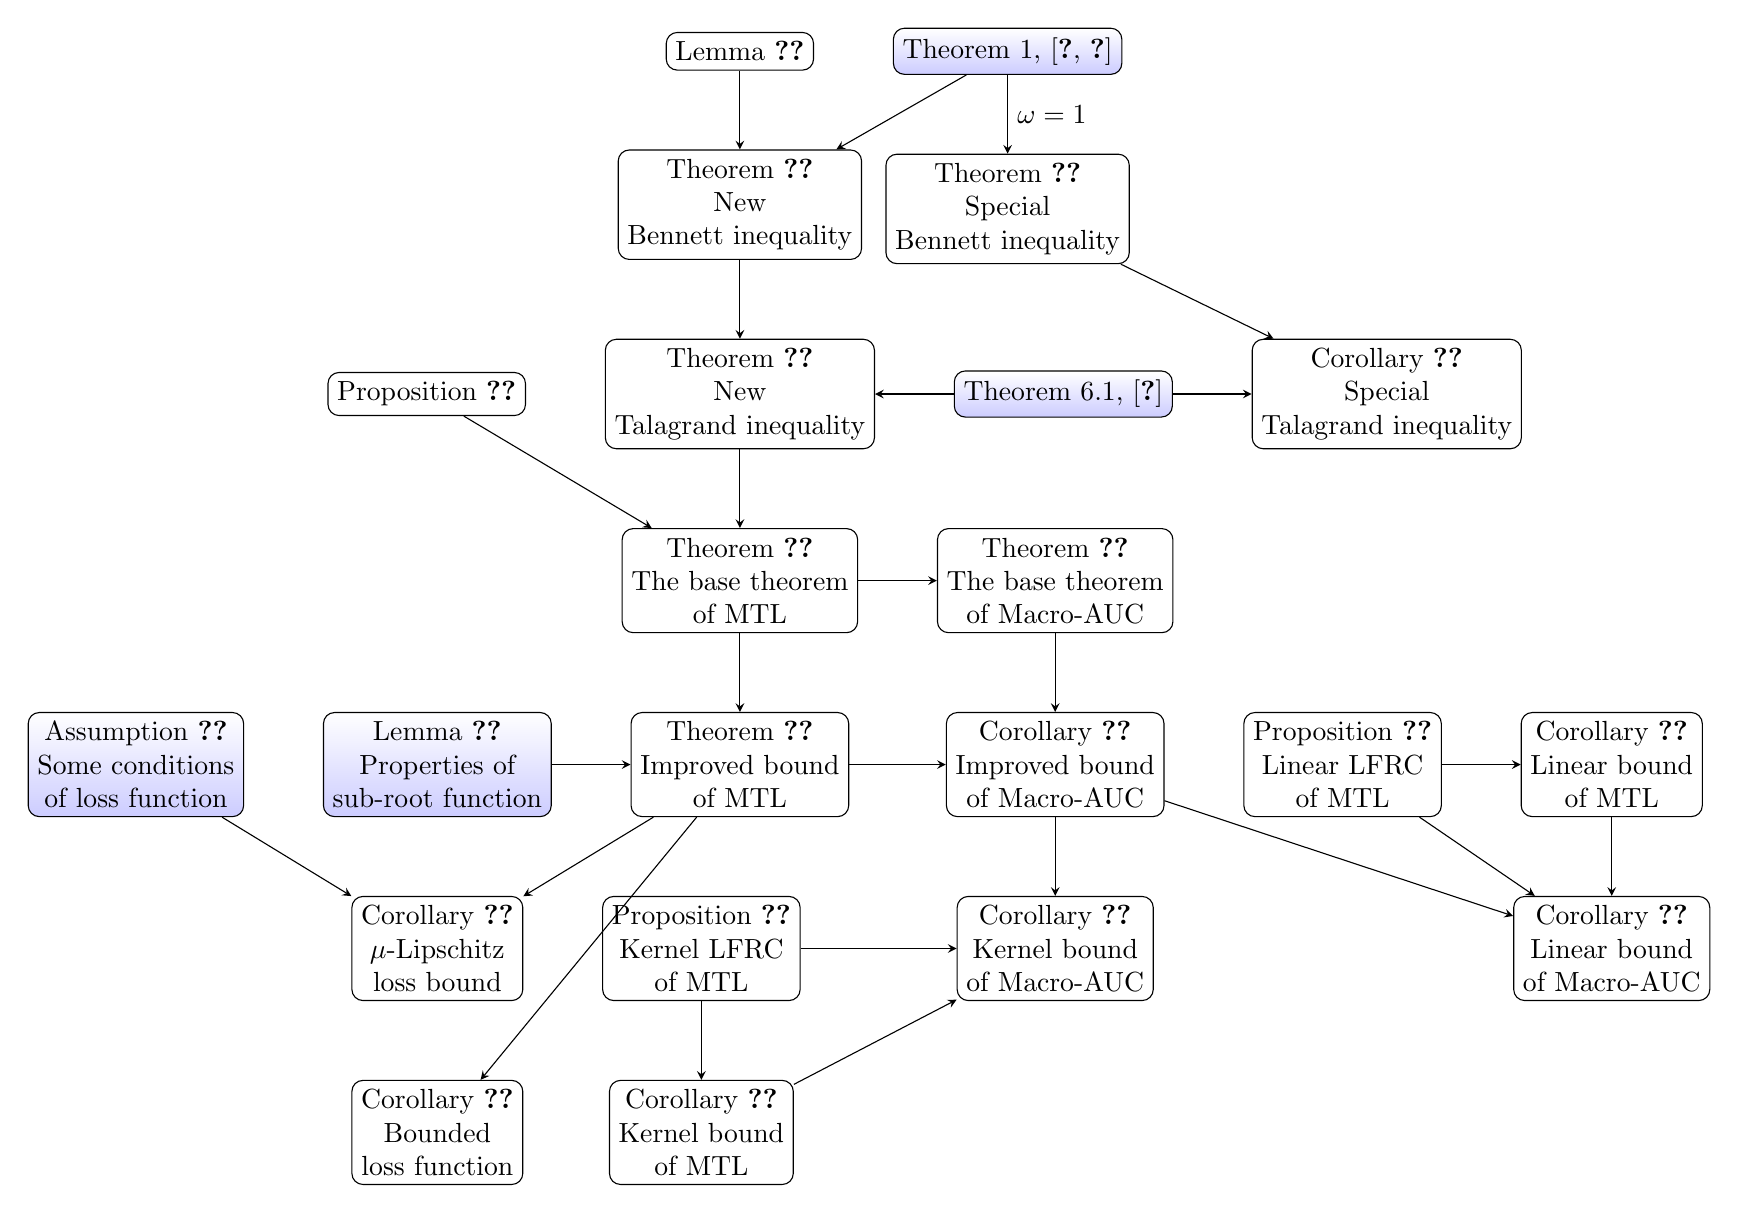
\begin{tikzpicture}[>=stealth,
        old/.style={shape=rectangle,align=center,draw,rounded corners, top color=white, bottom color=blue!20},
        new/.style={shape=rectangle,align=center,draw,rounded corners}
        ]
    % create the nodes
    \node[new] (n1) {Lemma~\ref{pro: inequality technique}};
    \node[old] (n2) [right = of n1]
    {Theorem~1, \cite{bousquet2002bennett,bousquet2003concentration}};
    \node[new] (n3) [below = of n1]
    {Theorem \ref{thm:bennett_inequality}\\
    New \\ Bennett inequality};
    \node[new] (n4) [below = of n2] {Theorem~\ref{thm:bennett_inequality_refined}\\
    Special \\ Bennett inequality};
    \node[new] (n5) [below = of n3] {Theorem~\ref{thm:talagrand_inequality}\\
    New \\ Talagrand inequality};
    \node[old] (n6) [right = of n5] {Theorem~6.1, \cite{bousquet2003concentration}};
    \node[new] (n7) [right = of n6] {Corollary~\ref{thm:talagrand_inequality_refined}\\
    Special \\ Talagrand inequality};
    \node[new] (n8) [below = of n5] {Theorem~\ref{thm:the core 2.1}\\
    The base theorem \\ of MTL};
    \node[new] (n9) [left = of n5] {Proposition~\ref{pro: equ Rademacher}};
    \node[new] (n10) [right = of n8] {Theorem~\ref{thm: base auc}\\
    The base theorem \\ of Macro-AUC};
    \node[new] (n11) [below = of n8] {Theorem~\ref{thm: theorem 3.3 sub-root}\\
    Improved bound \\ of MTL};
    % \node[old] (n12) [below = of n9] {Definition~\ref{lemma: sub-root def}\\
    % Sub-root function};
    \node[old] (n13) [left = of n11] {Lemma~\ref{lemma:sub-root pro}\\
    Properties of \\ sub-root function};
    \node[new] (n14) [below = of n13] {Corollary~\ref{thm : Lipschitz bound loss space}\\
    $\mu$-Lipschitz \\ loss bound};
    \node[old] (n15) [left = of n13] {Assumption~\ref{thm:assump2}\\
    Some conditions \\ of loss function};
    \node[new] (n16) [below = of n14] {Corollary~\ref{thm: general loss bound}\\
    Bounded \\ loss function};
    \node[new] (n17) [below = of n10] {Corollary~\ref{thm: sub-root AUC}\\
    Improved bound \\ of Macro-AUC};
    \node[new] (n18) [right = of n14] {Proposition~\ref{thm:kernel upper bound}\\
    Kernel LFRC \\ of MTL};
    \node[new] (n19) [below = of n18] {Corollary~\ref{thm: loss bound computing}\\
    Kernel bound \\ of MTL
    };
    \node[new] (n20) [below = of n17] {Corollary~\ref{thm: kernel comput AUC}\\
    Kernel bound \\ of Macro-AUC};
    \node[new] (n21) [right = of n17] {Proposition~\ref{thm:linear upper bound}\\
    Linear LFRC \\ of MTL};
    \node[new] (n22) [right = of n21] {Corollary~\ref{thm: loss bound computing2}\\
    Linear bound \\ of MTL};
    \node[new] (n23) [below = of n22] {Corollary~\ref{thm: linear comput AUC}\\
    Linear bound \\ of Macro-AUC};    

           
    % connect the nodes
    \draw[->] (n1) -- (n3);
    % \draw[->] (A) -- node[right] {w = 1} (B);
    \draw[->] (n2) -- node[right] {$\omega=1$} (n4);
    \draw[->] (n3) -- (n5);
    \draw[->] (n2) -- (n3);
    \draw[->] (n6) -- (n5);
    \draw[->] (n6) -- (n7);
    \draw[->] (n5) -- (n8);
    \draw[->] (n8) -- (n11);
    \draw[->] (n4) -- (n7);
    \draw[->] (n8) -- (n10);
    \draw[->] (n9) -- (n8);
    % \draw[->] (n12) -- (n11);
    \draw[->] (n13) -- (n11);
    \draw[->] (n11) -- (n17);
    \draw[->] (n11) -- (n14);
    \draw[->] (n11) -- (n16);
    \draw[->] (n15) -- (n14);
    \draw[->] (n17) -- (n23);
    \draw[->] (n17) -- (n20);
    \draw[->] (n18) -- (n20);
    \draw[->] (n19) -- (n20);
    \draw[->] (n18) -- (n19);
    \draw[->] (n21) -- (n23);
    \draw[->] (n21) -- (n22);
    \draw[->] (n22) -- (n23);
    \draw[->] (n10) -- (n17);


        \end{tikzpicture}
        % \caption{Main results framework diagram. The blue node denotes previous results (or assumptions) and others are our contributions.}
        \caption{The proof structure diagram of the main results. The blue node denotes previous results (or assumptions) and others are our contributions.}
        \label{fig:theorem proof}
    \end{figure}



\section{Additional Concentration Inequalities
% \guoqiang{is this name suitable, should be Additional Concentration Inequalities?}
}

\label{section: G}

This section serves as a supplement to Section \ref{section: main results}, discussing specific cases of the new Bennett inequality proposed in this paper, as well as some direct applications, such as the Talagrand inequality.
\subsection{A Special Bennett's Inequality}
\label{sec-app:a_special_bennett_inequality}
    \begin{theorem}[A new refined Bennett's inequality for a special case of multi-graph dependent variables, proof in Appendix \ref{pro:theorem4_proof}]
    \label{thm:bennett_inequality_refined}
    $Z = \sum_{k \in [K]} \sum_{j \in [J_k]} \omega_{kj}Z_{kj} $ (see details in Eq. \eqref{def :Z def}, Section \ref{section: main results}).  
    % \xiao{need change}. 
    Suppose Assumption \ref{thm:assump1} holds, and for every $k \in [K], j \in [J_k]$,  $b_{kj}=b, ~\omega_{kj}=1$. Then 
        % Suppose Assumption~\ref{thm:assump1} holds with $b_{k1} = ... = b_{kJ_k} = b$, $\omega_{kj} = 1, ~\forall k \in [K],~ \forall j \in J_k$, and define the constants

% \xiao{some appendix}
        
        % \begin{align*}
        %     & \sigma^2 = \sum_{k \in [K]} \sum_{j \in [J_k]} \omega_{kj} \sigma_{kj}^2, \ v = (1 + b) \eE [Z] + \sigma^2, \\
        %     & c = \sum_{k \in [K]} \chi_{f} (G_k), \ \chi_{f} (G_k) \defeq \sum_{j \in [J_k]} \omega_{kj} .
        % \end{align*}
        % Then, the following results hold:
        \begin{enumerate}[(1)]
            \item for every $t > 0$,
                \begin{align}
                \label{eq:thm_bennet_1_new}
                    \pP (Z \geq \eE[Z] + t) \leq \exp \left( - v \varphi \left( \frac{t}{v { \sum_{k \in [K]} \chi_{f} (G_k)} } \right) \right) ,
                \end{align}
% \xiao{need change}                
            where $v = (1 + b) \eE [Z] + \sigma^2$, $W = \sum_{k \in [K]} \chi_f(G_k) = \sum_{k \in [K]} \omega_k$, and $\omega_k = |J_k|$, $U = \sum_{k \in [K]}$. Additionally,  $\varphi$ can be seen in  Eq.\eqref{eq:psi_function}, i.e., $\varphi(x) = (1+x) \log(1+x)-x$;
            \item for every $t > 0$,
                \begin{align}
                \label{eq:thm_bennet_2_new}
                    % \pP (Z \geq \eE[Z] + \sqrt{2cvt} + \frac{2ct}{3}) \leq e^{-t} .
                    \pP (Z \geq \eE [Z] + c \sqrt{2vt} + \frac{2ct}{3}) \leq e^{-t} ,
                \end{align}
                where $c = \sum_{k \in [K]} \chi_{f} (G_k)$ (details in Appendix \ref{section: B}).  
        \end{enumerate} 
        % \xiao{need change}

    \end{theorem}
\begin{remark}
    This theorem serves as a complement to Theorem \ref{thm:bennett_inequality} and represents a specific instance of the Bennett inequality, applicable to i.i.d random variables. A detailed analysis and discussion of its implications will follow.
\end{remark}
Discussion:
then we discuss the above inequality in two cases, and in contrast to the i.i.d. case \cite{Bartlett_2005,yousefi18,watkins2023optimistic} and the single graph \cite{ralaivola2015entropy}. 
% (Proof in Appendix \ref{section: B})
\begin{enumerate}[(1)]
    \item in the i.i.d. case, $\chi _f(G_k) = \chi _f(G) = 1 $, we take $K = 1$ to contrast to single-graph, \\
    the result in the single-graph case is  
    \begin{align*}
       \pP (Z - \eE Z \geq t) \leq e^{-\frac{v}{\chi _f(G)} \varphi (\frac{4t}{5v})} = e^{-v \varphi (\frac{4t}{5v})}, 
    \end{align*}
    while our result is  
    \begin{align*}
        \pP (Z - \eE Z \geq t) \leq e^{-v \varphi (\frac{t}{v \sum _{k \in [K]} \chi _f(G_k)})} = e^{-v \varphi (\frac{t}{v})}.
    \end{align*} 
For a fixed $t$, we observe that the smaller $ \pP (Z - \eE Z \geq t) $ this term, the better. Since $\varphi (\frac{t}{v}) > \varphi (\frac{4t}{5v})$, $e^{-v \varphi (\frac{t}{v})} < e^{-v \varphi (\frac{4t}{5v})}$, our bound is tighter, and Bennett's inequality in prior work can be viewed as a special case. 
% For a fixed $t$, we observe that a smaller value of 
% \xiao{the work \cite{watkins2023optimistic} is the multi-function edition Bernstein inequality, which has the same result with \cite{Bartlett_2005}.}

    \item in the graph-dependent case, $\chi_f(G) \neq 1$, we also take $K =1$ to contrast to the single-graph. In this case, $\sum _{k \in [K]} \chi _f(G_k) = \chi _f(G) \geq 2$,  \\
    the result in \cite{ralaivola2015entropy} is  
    \begin{align*}
       \pP (Z - \eE Z \geq t) \leq e^{-\frac{v}{\chi _f(G)} \varphi (\frac{4t}{5v})}, 
    \end{align*}
    while our result is  
    \begin{align*}
        \pP (Z - \eE Z \geq t) \leq e^{-v \varphi (\frac{t}{v \sum _{k \in [K]} \chi _f(G_k)})} = e^{-v \varphi (\frac{t}{v \chi _f(G)})}.
    \end{align*}

Denote $\clubsuit _1 = -\frac{v}{\chi _f(G)} \varphi (\frac{4t}{5v}) $, and $ \clubsuit _2 = -v \varphi (\frac{t}{v \chi _f(G)}) $, $c_1 = \frac{1}{\chi _f(G)}$, $c_2 = \frac{4}{5}$, $x = \frac{t}{v}$, then
\begin{align*}
    \clubsuit_1 - \clubsuit _2 
    = &  v \varphi (c_1 x) - c_1 v \varphi (c_2 x) 
    =  v (\varphi (c_1 x) - c_1 \varphi(c_2 x) ) \\ 
    = & (1 +c_1 x)\log (1+c_1 x)   -  c_1(1 +c_2x) \log (1+ c_2 x) - (c_1 - c_1 c_2)x.
\end{align*}
We can notice that as $\chi _f(G)$ increases, $\clubsuit _1 - \clubsuit_2 $ becomes smaller and smaller, i.e., $\clubsuit _1 - \clubsuit _2 \approx 0 $. Thus our result in Theorem \ref{thm:bennett_inequality_refined} is equivalent to the result in \cite{ralaivola2015entropy}. 

\end{enumerate}

% \subsection{A new Talagrand's inequality}
%     \begin{theorem}[A new corresponding Talagrand’s inequality for empirical process, proof in Appendix \ref{section: A}]
%     \label{thm:talagrand_inequality}
%         Denote $\mX$ as some random variables, which are divided in the same way as the Section \ref{section: preliminaries}, i.e., $\mX = (\mX_1, \dots, \mX_K)$, and for every $k \in [K]$, $\mX_k = (\vx_{k1}, \dots, \vx_{k m_k})$, with $m = \sum_{k \in [K]} m_k$. Assume that each $\mX_k$ is related to a dependence graph $G_k$, where ${ (I_{kj}, \omega_{kj}) }_{j \in [J_k]}$ constitutes a fractional independent vertex cover of $G_k$, and define $\chi_f (G_k) \defeq \sum_{j \in [J_k]} \omega_{kj}$.  

% Let function class $\mathcal{F} = \{ f = (f_1, f_2, \ldots, f_K) \}$, where each $f_k: \mathcal{X} \rightarrow \mathcal{Y}$, and assume that all functions $f_k$ are measurable, square-integrable, and fulfill the conditions $\mathbb{E} [f_k(\vx_{kj})] = 0$ for all $k \in [K]$ and $j \in [m_k]$. Furthermore, we require that $\|f_k\|_{\infty} \leq 1$.
% Define $Z$ as follows:
%     \begin{align*}
%         Z \defeq \sup_{f \in \mathcal{F}} \sum_{k \in [K]} \sum_{j \in [J_k]} \omega_{kj}  \sum_{i \in I_{kj}} f_k(\vx_i).
%     \end{align*}

% Moreover, for every $k \in [K],~j \in [J_k]$, donate a positive real value $\sigma_{kj}$, satisfying $\sigma_{kj}^2 \geq \sum_{i \in I_{kj}} \sup_{f \in \mathcal{F}} \eE[f^2(\vx_i)]$. Then, for every $t \geq 0$,

% \begin{align}
%     \pP (Z \geq \eE[Z] + t) \leq \exp \left( - \frac{v}{ \sum_{k \in [K]} \chi_{f} (G_k)} \varphi \left( \frac{4t}{5v}\right) \right) ,
% \end{align}
%         where $v = \sum_{k \in [K]} \sum_{j \in [J_k]} \omega_{kj} \sigma_{kj}^2 + 2 \eE [Z]$, and the definition of $\chi_{f}(G_k), ~\varphi(x)$ is similar to Theorem \ref{thm:bennett_inequality}. 
%         Also, with probability at least $1 - e^{-t}$,
%         \begin{align}
%             Z \leq \eE[Z] + \sqrt{2cvt} + \frac{2ct}{3} , 
%         \end{align}
%         where $c = \frac{5^2}{4^2} \sum_{k \in [K]} \chi_{f} (G_k)$.
%     \end{theorem}
% (Proof in Appendix \ref{section: A})
Similar to Theorem \ref{thm:talagrand_inequality}, we can derive the special Talagrand-type inequality from Theorem \ref{thm:bennett_inequality_refined}.


\subsection{A Special Talagrand-type Inequality}
\label{sec-app:special_talagrand_inequality}
\begin{corollary} [A new refined Talagrand-type inequality for empirical process with a special case of  multi-graph dependent variables, proof in Appendix \ref{section: A}]
\label{thm:talagrand_inequality_refined}
    Denote $\mX$ as some random variables, which are divided in the same way as the Section \ref{section: preliminaries}, i.e., $\mX = (\mX_1,\mX_2,\dots,\mX_K)$. For every $k \in [K]$, $\mX_k = (\vx_{k1},\vx_{k2},\dots,\vx_{k m_k})$, with $m=\sum_{k \in [K]}m_k$. Assume that each $\mX_k$ is linked to a dependence graph $G_k$, where $\{ (I_{kj}, \omega_{kj}) \}_{j \in [J_k]}$ constitues a fractional independent vertex cover of $G_k$, and define $\chi_{f} (G_k) \defeq \sum_{j \in [J_k]} \omega_{kj}$.
        % Let $\mX = (\mX_1, \dots, \mX_K)$ be random variables where for each $k \in [K]$, $\mX_k = (\vx_{k1}, \dots, \vx_{k m_k})$ in which each $j \in [m_k]$, $\vx_{kj}$ is sampled from a distribution $P_k$ over $\mathcal{X}$ and $m = \sum_{i \in [K]} m_k$. Assume for each $k \in [K]$, $\mX_k$ is associated with a dependence graph $G_k$, where $\{ (I_{kj}, \omega_{kj}) \}_{j \in [J_k]}$ is a fractional independent vertex cover of $G_k$ and $\chi_{f} (G_k) \defeq \sum_{j \in [J_k]} \omega_{kj}$.
    
%         Let $\mathcal{F}$ be a set of functions from $\mathcal{X}$ to $\sR$ and assume all functions $f$ in $\mathcal{F}$ are measurable, square-integrable and satisfy $\eE [ f(\vx_{k j}) ] = 0, \omega_{kj}=1, \forall k \in [K], j \in [m_k]$ and $\| f \|_{\infty} \leq 1$. 
% \xiao{need some constants ...}

% Define:
% \begin{align*}
%     Z \defeq \sum _{k \in [K]} \sum _{j \in [J_k]} \omega_{kj} \sup _{f \in \mathcal{F}} \sum _{i \in I_{kj}} f_k(\vx_i)     
% \end{align*}

%next edition
% Let $\mathcal{F} = \{ f = (f_1,f_2,...f_K), f_k: \mathcal{X} \rightarrow \mathcal{Y} \}$, and assume all functions $f_k$ are measurable, square-integrable and satisfy $\eE [f_k(\vx_{kj})] = 0$, $w_{kj} = 1$, $\forall k \in [K], j \in [m_k]$ and $\|f_k\|_{\infty} \leq 1$.
Let $\mathcal{F} = \{ f, f = (f_1,\dots,f_K) \}$, where each $f_k: \mathcal{X} \rightarrow \mathcal{Y}$, and assume that all functions $f_k$ are measurable, squareintegrable, and fulfill the conditions $\eE [f_k(\vx_{kj})] = 0, ~\omega_{kj}=1$ for all $k \in [K]$ and $j \in [m_k]$. Additionally, we require that $\|f_k\|_{\infty} \leq 1$.
Define $Z$ as follows:
    \begin{align*}
        Z \defeq \sup_{f \in \mathcal{F}} \sum_{k \in [K]} \sum_{j \in [J_k]}  \sum_{i \in I_{kj}} f_k(\vx_i).
    \end{align*}

% \xiao{don't need to write detail}
% and we also need to discuss the following: 
% \begin{align*}
%     Z \defeq  \sup _{f \in \mathcal{F}} \sum _{k \in [K]} \frac{1}{m_k} \sum _{j \in [J_k]} \sum _{i \in I_{kj}} f(\vx_i)    
% \end{align*}

% Let $\sigma_{kj}$ be a positive real number such that $\sigma_{kj}^2 \geq \sum_{i \in I_{kj}} \sup_{f \in \mathcal{F}} \eE[f^2(x_i)]$. Then, for any $t \geq 0$, 
Moreover, for every $k \in [K]$, $j \in [J_k]$, donate a positive real value $\sigma_{kj}$, satisfying $\sigma_{kj}^2 \geq \sum_{i \in I_{kj}} \sup_{f \in \mathcal{F}} \eE[f^2(\vx_i)]$. Then, for every $t \geq 0$,
\begin{align}
     \pP (Z \geq \eE[Z] + t) \leq \exp \left( - v \varphi \left( \frac{t}{v W}\right) \right) ,
\end{align}
where $v = \sum_{k \in [K]} \sum_{j \in [J_k]} \sigma_{kj}^2 + 2 \eE [Z]$, $W = \sum _{k \in [K]} \chi _f(G_k) $, and the definition of other variables in Theorem \ref{thm:bennett_inequality_refined}. 
Also, with probability at least $1 - e^{-t}$,
\begin{align}
Z \leq \eE[Z] + c \sqrt{2vt} + \frac{2ct}{3} , 
\end{align}
where $c = \sum_{k \in [K]} \chi_{f} (G_k)$.

    \end{corollary}
% \xiao{now we can proof the corollary \ref{thm:talagrand_inequality_refined}} \\

% Similarly, we can use the Theorem \ref{thm:bennett_inequality_refined} and the Theorem 6.1 in \cite{bousquet2003concentration} to get the results, and we can observe $b = 1$.  

\begin{remark}
    This result is specific to Theorem \ref{thm:talagrand_inequality} and represents an inequality directly derived from Theorem \ref{thm:bennett_inequality_refined}. It can be used to further develop the form of LRC and applies to the generalized boundary analysis of MTL, encompassing the case of i.i.d. (detail information and in \ref{section: A}). 
\end{remark}

\subsection{Supplement to Bennett Inequality}
\label{sec-app:supplement-bennett-lower}
\begin{theorem}[The lower bound of Bennett's inequality for a special case of multi-graph dependent variables] \label{thm: bennett inequality lower bound}
Given $Z = \sum_{k \in [K]} \sum_{j \in [J_k]} \omega_{kj}Z_{kj} $ (see details in Eq.\eqref{def :Z def}, Section \ref{section: main results}).  Suppose Assumption \ref{thm:assump1} holds, and for every $k \in [K], j \in [J_k]$, $b_{kj}=b, ~\omega_{kj}=1$. Then for all $t>0$, 
\begin{align}
    \label{eq:thm_bennet_lower}
    \pP (Z \leq \eE[Z] - t) \leq \exp \left( - \frac{v}{W} \varphi \left( \frac{tW}{Uv} \right) \right) \leq \exp \left( -\frac{v}{\sum_{k \in [K]} \chi_f(G_k) } \varphi \left(\frac{4t}{5v} \right) \right) ,
\end{align}
where $\varphi$ is defined as above, i.e., $\varphi(x)=(1+x) \log(1+x)-x$. Owing to the fact $x \geq 0$, $\varphi(x) \geq \frac{x^2}{2+ \frac{2x}{3}}$, we can get 
\begin{align}
    \label{eq:thm-bennett_lower2}
    \pP (Z \leq \eE [Z] - \sqrt{2cvt} - \frac{2ct}{3}) \leq e^{-t},
\end{align}
where $c = \frac{5^2}{4^2} \sum_{k \in [K]} \chi_f(G_k)$. The definition of $v,~W,~U$ can be seen in Theorem \ref{thm:bennett_inequality}.      
\end{theorem}

\begin{remark}
    This theorem supplements the Bennett inequality and can be used to analyze the lower bounds of the generalization bounds discussed later. Furthermore, this theorem can be combined with the results of Theorem \ref{thm:bennett_inequality}, then $\pP (|Z - \eE [Z]| \geq t) \leq 2 \exp ( -\frac{v}{\sum_{k \in [K]} \chi_f(G_k)} \varphi (\frac{4t}{5v} ) )$. The equivalence of the upper and lower bounds implies that the bound obtained is relatively tight. However, the result does not cover the i.i.d. case. This indicates that the result is not optimal and that there is still a gap $\frac{5}{4}$  to be bridged.
\end{remark}

\begin{proof}
    We can define some constants as Theorem \ref{thm:bennett_inequality}, then
    \begin{align*}
        \pP (Z - \eE[Z] \leq -t) = \pP (\eE[Z] - Z \geq t) = \pP (e^{\lambda (\eE[Z]-Z)} \geq e^{\lambda t}) \leqone \eE(e^{\lambda (\eE[Z]-Z)}) \cdot e^{-\lambda t},
    \end{align*}
\text{\ding{172}} is owing to the fact, i.e.,  $\forall a >0,~ \pP [x >a] \leq \frac{\eE[X]}{a}$. The result can then be obtained using the same technique as in the proof of Theorem \ref{thm:bennett_inequality}. 
\end{proof}

\section{Theoretical Results for MTL with Multi-graph Dependent Data} 
% \section{Theoretical Results for MTL, Data with Dependent Graph} 
\label{section: MTL gereral bound}

In this section, we will provide some results on the generalization bounds of MTL in the case of graph-dependent case, to supplement the content of Section \ref{section: main results} in the main text.
\subsection{Supplemental definition and proposition}
\begin{definition}[The LFRC of the loss space]
    Define $\mathcal{H}=\{ h = (h_1,h_2,...,h_K) | h_k: \mathcal{X} \rightarrow \widetilde{\mathcal{Y}}, k \in [K] \}$ as the hypothesis space, $\mathcal{H}_k = \{ h_k: \mathcal{X} \rightarrow \widetilde{\mathcal{Y}} \}$, and $L : \mathcal{X} \times \mathcal{Y} \times \mathcal{H}_k \rightarrow \sR^+$, $L \in [0,M_c]$. According to Definition \ref{def: LFRC}, the empirical LFRC of loss space is defined as
    % \begin{small}
    %     \begin{align*}
    %         & \hat{\mathcal{R}}_S (L \circ \mathcal{F}) \\
    %         & = \frac{1}{K} \eE _\zeta \left[ \sup _{f \in \mathcal{F}, \mathrm{var}(f) \leq r} \sum _{k \in [K]} \frac{1}{m_k}   \sum _{j \in J_k} \omega_{kj}  \sum _{i \in I_{kj}} \zeta_i L(x_i,y_i,f_k)   \right].
    %     \end{align*}        
    % \end{small}
    \begin{align*}
        \hat{\mathcal{R}}_S (L \circ \mathcal{H}) = \frac{1}{K} \eE _\zeta \left[ \sup _{h \in \mathcal{H}, \mathrm{var}(h_k) \leq r} \sum _{k \in [K]} \frac{1}{m_k}   \sum _{j \in J_k} \omega_{kj}  \sum _{i \in I_{kj}} \zeta_i L(x_i,y_i,h_k)   \right].
    \end{align*}        

    Furthermore, the LFRC of $L \circ \mathcal{H}$ is defined as
    \begin{align*}
        \mathcal{R}_m (L \circ \mathcal{H}) = \eE _{S \sim D^m_{[K]}} [\mathcal{R}_S(L \circ \mathcal{H})].
    \end{align*}    
\end{definition} 

\begin{proposition} \label{pro: equ Rademacher}
% \guoqiang{to give a name, the contraction inequality?}
For every $ r > 0 $, 
\begin{align}
    \eE _{S,S'}  \sup _{f \in \mathcal{F}} \sum _{k \in [K]} \sum _{j \in [J_k]}  \frac{\omega_{kj}}{K m_k}  \sum _{i \in I_{kj}} ( f_k(\vx'_i) - f_k(\vx_i)) \leq 2 \mathcal{R} (\mathcal{F},r) .
\end{align}

\end{proposition}
we can prove this inequality due to the property of the Rademacher Complexity and the symmetry.  
\subsection{Supplemental risk bounds}
\label{sec-app:supplemental-risk-bounds}
\begin{corollary}[An excess risk bound of learning multiple tasks with graph-dependent examples, proof in Appendix~\ref{section: A}] \label{thm: general loss bound}
    Let \( \hat{h} \) and \( h^* \) denote the prediction functions, which correspond to the minimum empirical loss and the minimum expected loss, respectively.
    % For every $k \in [K], j \in J_k, \eE[f(\vx_{kj})] = 0$, $\|f \|_\infty \leq 1$, and 
    Assume a bounded loss function $ L \in [0, M_c] $. Assume:

    a sub-root function $\Phi$ and its fixed point $r^*$ satisfied the following: 
    \begin{align*}
        \forall r \geq r^*,~  \Phi (r) \geq M_c \mathcal{R} \{ h \in \mathcal{H}, \eE (L_{h_k} - L_{h_k^*})^2 \leq r \}.
    \end{align*}
    Then for every $t > 0$, with probability at least $1 - e^{-t}$, 
    \begin{align} \label{eq: collary 5.1 bounded loss}
        P (L_ {\hat{h}} - L_{h^*}) \leq \frac{c_1 }{M_c} r^* + (c_2 M_c  + 22) \frac{ct}{K},  
    \end{align}
    where $c_1 = 704$, $c_2 = 26$, and $c = \frac{5^2}{4^2} \sum_{k \in K}\frac{\chi_f(G_k)}{m_k} $. 
\end{corollary}

This corollary gives the risk bound of a general bounded loss function, which can be improved if some properties of the loss function and the hypothesis class are taken into account. 
% (Proof in Appendix \ref{section: A}).
\begin{proposition}[The upper bound of LFRC of the kernel hypothesis space, proof in Appendix \ref{pro:proposition1_proof}] \label{thm:kernel upper bound}
% Assume $f = \Theta^T \Phi(\vx)$, where $\Theta = (\theta_1,\dots,\theta_K)^T$, $\|\theta_k\|_2 \leq \widetilde{M}$, $\Phi$, 
% and for each $k \in [K]$, $\|\theta_k\|_* \leq \widetilde{M}$, $f_k = \theta_k^T \phi(\vx_k)$.
% \guoqiang{what is $\|H_k\|$?} \guoqiang{$\Theta, \theta$} 
Define $\kappa: \mathcal{X} \times \mathcal{X} \rightarrow \sR$ as a Positive Definite Symmetric (PDS) kernel and let its induced reproducing kernel Hilbert space (RKHS) be $\mathbb{H}$. Assume for every $k \in [K]$, $f_k = \theta_k^T \phi(\vx_k)$, where a weight vector satisfies $\|\theta_k\|_2 \leq \widetilde{M}$, and $\phi: \mathcal{X} \rightarrow \mathbb{H}$. 
For every $r >0$, the LFRC of function class $\mathcal{F}$ satisfies 
    \begin{align*}
        \mathcal{R}\{ f \in \mathcal{F}, \eE f_k^2 \leq r \}  
        \leq \sum _{k \in [K]} \left(\frac{2 \chi_f(G_k)}{K m_k} \sum _{l=1}^{\infty} \min \{ r, \widetilde{M}^2 \lambda_{kl} \} \right)^{\frac{1}{2}},
    \end{align*}
% \guoqiang{$ \eE f^2 \leq r $ or $ \eE f_k^2 \leq r $?}
where for every $k \in [K]$, the eigenvalues $(\lambda _{kl})_{l=1} ^{\infty}$
% \guoqiang{notation has a problem}
are arranged in a nonincreasing order, which satisfies $\kappa_k (\vx,\vx') = \sum _{l =1} ^{\infty} \lambda_{kl} \varphi_{kl}(\vx)^T \varphi _{kl}(\vx') $. 

Moreover, if for every $k \in [K]$, $\lambda_{k 1} \geq \frac{1}{m_k \widetilde{M}^2}$. 
% \guoqiang{$\lambda_{k 1}$ or $\lambda_{k l}$}, 
Then for every $r \geq \frac{1}{m}$ and $m=\sum_{k \in [K]} m_k$, 
\begin{align*}
    \mathcal{R}\{ f \in \mathcal{F}, \eE f_k^2 \leq r \}  
    \geq c \sum _{k \in [K]} \left(\frac{ \chi_f(G_k)}{K m_k} \sum _{l=1}^{\infty} \min \{ r, \widetilde{M}^2 \lambda_{kl} \}\right)^{\frac{1}{2}},
\end{align*}
where $c$ is a constant. 
% The inequality gives the lower bound of LFRC in the kernel space.\guoqiang{this sentence is redundant.} 
\end{proposition}

\begin{remark}
    This proposition indicates the upper bound of $\mathcal{R}(\mathcal{F},r)$ is tight since it matches the order of its lower bound.
    % This proposition provides both upper and lower bounds for $\mathcal{R}(\mathcal{F},r)$ . The upper bound is relatively tight, while the lower bound is more approximate. Nevertheless, these results can still give a rough indication of the complexity bounds of $\mathcal{R} (\mathcal{F},r)$. \guoqiang{what want to say?}
    % The above establishes a more specific bound for the LFRC within the kernel hypothesis space. In this context, we will subsequently explore the relationship between the fixed point of the sub-root function and $\mathcal{R}(\mathcal{F}_{l,r})$, aiming to obtain a more specific risk bound. 
    % (Proof in Appendix~\ref{section: B})
\end{remark}

\begin{proposition}[The upper bound of LFRC in linear hypothesis, proof in Appendix \ref{pro:proposition3_proof}]
\label{thm:linear upper bound} Assume that $\sup _{\vx \in \mathcal{X}} \|\vx\|_2^2 \leq \bar{M}^2$, $\bar{M} >0$. The function class $\mathcal{F} = \{ f, f = (f_1,f_2,\dots,f_K), f_k = \theta_k^T \vx_k, \|\theta_k\|_2 \leq \widetilde{M} \}$. For every $ r >0$, 
    \begin{align*}
       & \mathcal{R}\{ f \in \mathcal{F}, \eE f_k^2 \leq r \} \leq \sum _{k \in [K]} \left( \frac{2 \chi_f(G_k)}{K m_k} \sum _{kl = 1} ^{\infty} \min \{ \frac{r}{\bar{M}^2} , \widetilde{M}^2 \widetilde{\lambda} ^2_{l} \} \right)^ {\frac{1}{2}}. \\
        % & \mathcal{R}\{ f \in \mathcal{F}, \eE f_k^2 \leq r \} \\ 
        % & \leq \left( \sum _{k \in [K]} \frac{2 \chi_f(G_k)}{m_k} \sum _{l = 1} ^{\infty} \min \{ \frac{r}{\bar{M}^2} , \widetilde{M}^2 \widetilde{\lambda} ^2_{l} \} \right)^{\frac{1}{2}},
    \end{align*}
where singular values $(\widetilde{\lambda}_l)_{l=1}^{\infty}$ in a nonincreasing order, and $\Theta = \sum_{l=1}^{\infty}u_l v_l^T \widetilde{\lambda}_l$, where $\Theta$ is a weight matrix. 

Moreover, if $\widetilde{\lambda}_1^2 \geq \frac{1}{m \widetilde{M}^2}$, then for every $r \geq \frac{\bar{M}^2}{m}$, $m = \sum_{k \in [K]} m_k$,
\begin{align*}
     \mathcal{R}\{ f \in \mathcal{F}, \eE f_k^2 \leq r \}  
     \geq c \sum_k \left(  \frac{ \chi_f(G_k)}{K m_k} \sum _{l = 1} ^{\infty} \min \{ \frac{r}{\bar{M}^2} , \widetilde{M}^2 \widetilde{\lambda} ^2_{l} \} \right)^{\frac{1}{2}},    
\end{align*}
where c is a constant. 
% The above gives the lower bound for linear space. 
\end{proposition}

\begin{remark}
    The above gives the upper and lower bounds for linear space.
    % A more refined upper bound for the LFRC within linear hypothesis spaces is presented here. 
    Furthermore, the relationship between this upper bound and the fixed point \( r^* \) is examined to facilitate a detailed analysis of the complexity associated with the generalization bound. 
    % (Proof in Appendix \ref{section: B})
\end{remark}


\begin{corollary}[An excess risk bound in linear hypothesis, proof in Appendix \ref{pro:corollary6_proof}]
\label{thm: loss bound computing2} Assume that $\sup _{\vx \in \mathcal{X}} $ $ \|\vx\|_2^2 \leq \bar{M}^2,\bar{M} > 0$, $\|\theta_k\|_2 \leq \widetilde{M}$, and loss function $L$ satisfies Assumption \ref{thm:assump2}, $C$ is a constant about $B, \mu $, and $C'$ is a constant about $\chi_f(G)$. Then for all $t > 0$,  with probability at least $1 - e^{-t}$, 
\begin{align}
    P (L_{\hat{h}} - L_{h^*}) \leq C_{B,\mu} (r^* + C'_{\chi_f(G)} \frac{t}{K}),
\end{align}
where
\begin{small}
    \begin{align} \label{eq:loss bound computing2 eq}
    r^* \leq \sum_k \min_{d \geq 0} ( \frac{d}{\bar{M}^2} \frac{\chi_f(G_k)}{K m_k} + \widetilde{M} \sqrt{ \frac{\chi_f(G_k)}{K m_k} \sum_{l > d} \widetilde{\lambda}_{l}^2 } ) ,
    \end{align}
\end{small}
where $d$ is the division of singular values of matrix $\Theta$, and $P (L_{\hat{h}} - L_{h^*})$ can be seen in Theorem \ref{thm : Lipschitz bound loss space}. 
\end{corollary}
% (Proof in Appendix \ref{section: B})

\section{Proofs} \label{section:proof_all}
In this section, we will give detailed proofs of some major theorems and corollaries, as well as some simple proof techniques for corollaries, so that readers can understand and sort out the main results.
\subsection{Proof Sketches} \label{section: A}
This section outlines the main ideas and techniques used in the proofs of several theorems and corollaries.

(1) Proof of Theorem \ref{thm:talagrand_inequality}, we can use Theorem 6.1 in \cite{bousquet2003concentration} and Theorem \ref{thm:bennett_inequality} to get the following: 
% we can use Theorem 6.1 in \cite{bousquet2003concentration} and the Theorem \ref{thm:bennett_inequality}, that is, we want to get the following, 
\begin{itemize}
    \item $ Y_{kjl} \leq Z_{kj}-Z_{kj}^{\backslash \{ l \} } \leq 1$, these inequalities are owing to 
    \begin{align*}
        & \sum_{i \in I_{kj} \backslash \{l \} } f_l^{kj}(\vx_i)  = \sup_{f \in \mathcal{F}} \sum_{i \in I_{kj} \backslash \{l \}} f(\vx_i), ~
         Y_{kjl} = f_l^{kj}(\vx_l),  \\
        & Y_{kjl} \leq Z_{kj}-Z_{kj}^{\backslash \{ l \} } \leq f_{kj}^*(\vx_l) \leq 1, ~
        \eE_{kjl} [Y_{kjl}] = 0. \\ 
    \end{align*}    

    \item $\sigma_{kj}^2 \geq \sum_{l \in I_{kj}} \eE _{I_{kj}} [Y_{kjl}^2]$, because
    \begin{align*}
        \sum_{l \in I_{kj}} \eE _{I_{kj}} [Y_{kjl}^2] = \sum_{l \in I_{kj}} \eE _{I_{kj}} [f_l^{{kj}^2}(\vx_l)] \leq \sum_{l \in I_{kj}} \sup_{f \in \mathcal{F}} \eE [f^2 \vx_l)].
    \end{align*}
\end{itemize}

(2) Proof of Corollary \ref{thm:talagrand_inequality_refined}, similar to above, we can use Theorem \ref{thm:bennett_inequality_refined} and Theorem 6.1 in \cite{bousquet2003concentration} to get the results, and we can observe $b = 1$. 

(3) Proof of Corollary \ref{thm: general loss bound}, let $g = L_{\hat{h}} - L_{h^*}$, $T(g_k) = \eE g_k^2$ and we notice $g_k \in [-M_c,M_c]$, 
then $\mathrm{var}(g_k) = \eE g_k^2 - (\eE g_k)^2 \leq \eE g_k^2$, i.e., $ \mathrm{var}(g_k) \leq T(g_k) $, $T(g_k) = \eE g_k^2 \leq M_c \eE g_k$,
then we can use Theorem \ref{thm: theorem 3.3 sub-root} to $g$, and since $P_m g  \leq 0$, we can omit the term $\frac{M}{M-1} P_m g$.

(4) Proof of Corollary \ref{thm : Lipschitz bound loss space}, according to Assumption \ref{thm:assump2}, then $\eE (L_{h_k} - L_{h_k^*})^2 \leq \mu^2 \eE (h_k - h_k^*)^2$, let $T(L_{h_k} - L_{h_k^*}) = \eE (L_{h_k} - L_{h_k^*})^2 \leq B \mu ^2 \eE (L_{h_k} - L_{h_k^*}) $, and we know $\mu \mathcal{R} \{ h,\mu^2 \eE(h_k - h_k^*) ^2 \leq r \} \geq \mathcal{R} \{ L_h - L_{h^*}, \mu ^2 \eE (h_k - h_k^*)^2 \leq r \}$. And we notice $P _m(L_{\hat{h}} - L_{h^*}) \leq 0 $, then use Theorem \ref{thm: theorem 3.3 sub-root} to get the results.

(5) Proof of Theorem \ref{thm: base auc}, we can use Theorem \ref{thm:the core 2.1} and the value of $m_k, 
 \chi_f(G_k)$, i.e., $m_k = \tilde{n}^2 \tau_k(1-\tau_k)$, $\chi_f(G_k) = (1- \tau_k)\tilde{n}$, to obtain the results. 

(6) Proof of Corollary \ref{thm: sub-root AUC}, we can prove the corollary by using Theorem \ref{thm: base auc} and Theorem \ref{thm: theorem 3.3 sub-root}, the value of $m_k, \chi_f(G_k)$, that is, $m_k = \tilde{n}^2 \tau_k(1-\tau_k)$, $\chi_f(G_k) = (1- \tau_k)\tilde{n}$.

(7) Proof of Corollary \ref{thm: kernel comput AUC}, we can use Corollary \ref{thm: sub-root AUC} and Proposition \ref{thm:kernel upper bound} (the upper bound of $r^*$), \ref{thm: loss bound computing} (the risk bound in the kernel hypothesis) to get the results and use the value of $m_k, \chi_f(G_k)$, i.e., $m_k = \tilde{n}^2 \tau_k(1-\tau_k)$, $\chi_f(G_k) = (1- \tau_k)\tilde{n}$. Also, if we use one kernel matrix, we can get $r^* \leq \min _{0 \leq d \leq m} \left(\frac{1}{\tilde{n}} \sum_{k \in [K]} \frac{1}{\tau_k} d + \widetilde{M} \sqrt{\frac{1}{\tilde{n}} \sum_{k \in [K]} \frac{1}{ \tau_k} \sum _{l >d} \lambda_{l}} \right)$. 

(8) Proof of Corollary \ref{thm: linear comput AUC}, we can use Corollary \ref{thm: sub-root AUC} and Proposition \ref{thm:linear upper bound} (the upper bound of $r^*$), \ref{thm: loss bound computing2} (the risk bound in linear hypothesis), and use the value of $m_k, \chi_f(G_k)$, i.e., $m_k = \tilde{n}^2 \tau_k(1-\tau_k)$, $\chi_f(G_k) = (1- \tau_k)\tilde{n}$. 
% Also, if we use the decomposition of H, we can get $r^* \leq \min _{0 \leq h \leq m} \left( \frac{1}{n} \cdot \frac{1}{\bar{M}^2} \sum_{k \in [K]} \frac{1}{\tau_k} h + \widetilde{M} \sqrt{ \frac{1}{n} \sum_{k \in [K]} \frac{1}{\tau_k} \sum _{l >h} \widetilde{ \lambda} _{l}^2} \right)$.

% (9) Proof of Corollary \ref{thm: loss bound computing own2}, we can use Theorem \ref{thm:multi own2 3.3}, and Proposition \ref{thm:kernel upper bound} to get the results.

% proof detail 
\subsection{Proof Details} 
\label{section: B}
% \label{sec:proof_details}
% proof of Bennet inequality (general)
This section provides a detailed explanation of the proof procedures for several key theorems and lemmas, aiming to facilitate understanding of their underlying reasoning.

\subsubsection{Proof of Theorem \ref{thm:bennett_inequality}}
\label{pro:bennett_inequ}
Here we give the proof of \textbf{Theorem \ref{thm:bennett_inequality} (A new Bennett's inequality for multi-graph dependent variables)}, 
and review $Z = \sum_{k \in [K]} \sum _{j \in [J_k]} \omega_{kj} Z_{kj} $, where $Z_{kj} = f_{kj}(x_{I_{kj}})$. 
% \guoqiang{the following expression follows this.} 
\begin{proof}
Define some constants as follows:
        \begin{align*}
            & \sigma^2 = \sum_{k \in [K]} \sum_{j \in [J_k]} \omega_{kj} \sigma_{kj}^2, \ v = (1 + b) \eE [Z] + \sigma^2, 
             c = \frac{5^2}{4^2} \sum_{k \in [K]} \chi_{f} (G_k), \ \chi_{f} (G_k) \defeq \sum_{j \in [J_k]} \omega_{kj} , \\
            & p_k = \frac{U_k}{U}, q_{kj} = \frac{\omega_{kj} \max (1, \overbrace{v_{kj}^{\frac{1}{2}} W^{\frac{1}{2}} v^{-\frac{1}{2}} } ^{\triangle})}{U_k}, 
             U = \sum_{k \in [K]} U_k, U_k = \sum_{j \in J_k} \omega_{kj} \max(1, \triangle), \\
            & W = \sum_{k \in [K]} \chi_f(G_k) = \sum_{k \in [K]} \omega_k,  
             \sigma _k^2 = \sum_{j \in I_{J_k}} \omega_{kj} \sigma _{kj}^2, \omega_k = \sum_{j \in [J_k]} \omega_{kj}, 
             v_k = \sum_{j \in [J_k]} \omega_{kj}v_{kj} = (1+b) \eE [Z_k] +\sigma _k^2. 
        \end{align*}
Then
    \begin{align*}
        \pP(Z-\eE Z \geq t) & = \pP(e^{\lambda (Z- \eE Z)} \geq e^{\lambda t}) \leqone \underbrace{  \eE(e^{\lambda (Z- \eE Z)}) }_{e^{G(\lambda )}} \cdot e^{-\lambda t}. \\
% \begin{center}
%     (According to Markov Inequality,$ \pP[x>a] \leq \frac{\eE[x]}{a} $)    
% \end{center}
       G(\lambda )  & = \log \eE (e^{\lambda (Z - \eE Z)}) \\
        & = \log \eE (e^{\lambda \sum _{k \in [K]}p_k \frac{1}{p_k}  (Z_k - \eE _{X_k} [Z_k] )})  \\
        & = \log \eE (e^{\lambda \sum _{k \in [K]}p_k \frac{1}{p_k} \sum _{j \in [J_k] } q_{kj} \frac{\omega_{kj}}{q_{kj}}  (Z_{kj} - \eE _{X_{I_{kj}}}  [Z_{kj}] )}) \\
        & \leqtwo  \log \sum_{k \in [K]}p_k\sum_{j \in [J_k]}q_{kj} 
        \eE(e^{\frac{\lambda \omega_{kj}}{p_k q_{kj}}(Z_{kj}- \eE [Z_{kj}]) }) ,\\   
% \begin{center}
%    {(according to Jensen inequality)}   
% \end{center}
        G_{kj}(\lambda ) & = \log \eE (e^{\lambda (Z_{kj}- \eE Z_{kj})}), \\
        G(\lambda ) & \leqthree \log \sum_{k \in [K]}p_k\sum_{j \in [J_k]}q_{kj} (e^{ G_{kj} ({\frac{\lambda \omega_{kj}}{p_k q_{kj}} })}) \\
        & \leqfour \log \sum_{k \in [K]}p_k\sum_{j \in [J_k]}q_{kj} (e^{ v_{kj} \psi (-{\frac{\lambda \omega_{kj}}{p_k q_{kj}} })}).
    \end{align*}

\text{\ding{172}} is due to the Markov Inequality, i.e., $\pP [x > a] \leq \frac{\eE[x]}{a}$, and we define $e^{G(\lambda) } = \eE (e^{\lambda (Z - \eE Z)}) $. \text{\ding{173}} is due to the Jensen inequality, and \text{\ding{174}} is due to the assumption \ref{thm:assump1}, the last inequality \text{\ding{175}} is due to Theorem 1 \cite{bousquet2002bennett,bousquet2003concentration}, i.e., $G(\lambda) \leq \psi(-\lambda)v $). We can observe that $ v_{kj} \psi (-{\frac{\lambda \omega_{kj}}{p_k q_{kj}} }) \leq \frac{v}{W} \psi (-\lambda U)$ (proof in Lemma~\ref{pro: inequality technique}),

then we have
\begin{align}
    \pP(Z-\eE Z \geq t) \leq e^{\frac{v}{W} \psi (-\lambda U) - \lambda t},
\end{align}
we solve the minimum optimization problem with respect to $\lambda$, for $\lambda = \frac{ln(1+\frac{tW}{vU})}{U}$, then
\begin{align}
    \pP (Z- \eE Z \geq t) \leq e^{-\frac{v}{W} \varphi (\frac{tW}{vU})}.
\end{align}

% then 
%     \begin{align*}
%         U_k & = \sum_{j \in [J_k]} w_{kj} \max (1,v_{kj}^{\frac{1}{2} }w_{k}^{\frac{1}{2}}v_k^{-\frac{1}{2} }) \\
%         & \leq \sum_{j \in [J_k]}w_{kj}(1+\frac{v_{kj}w_k}{4v_k} ) = \frac{5}{4}w_k ,\\
%         U & =\sum_{k \in [K]} U_k \max (1,(\frac{v_k}{w_k})^{\frac{1}{2} }W^{\frac{1}{2} }v^{-\frac{1}{2} } ) \\
%         & \leq \sum_{k \in [K]} U_k (1+\frac{v_k W}{4v w_k} ) \\
%         & \leq \frac{5}{4} \sum_{k \in [K]} w_k (1+\frac{v_k W}{4v w_k} ) = \frac{25}{16} W. \\  
%     \end{align*}

% \begin{center}
% (a technique, $\forall x \in \sR,x \leq 1 + \frac{x^2}{4} $)    
% \end{center}
Then
\begin{align*}
    U_k & =  \sum _{j \in [J_k]} w_{kj} \max (1, \triangle) \\
    & \leqone \sum _{j \in [J_k]} w_{kj} (1 + \frac{v_{kj} W}{4 v}) 
     = w_k + \frac{v_k W}{4v}, \\
    U & = \sum _{k \in [K]} U_k 
     = \sum _{k \in [K]} (w_k + \frac{v_k W}{4v}) 
     = W + \frac{W}{4} = \frac{5}{4}W,
\end{align*}
\text{\ding{172}} is according to the fact that $\forall x \in \sR,x \leq 1 + \frac{x^2}{4}$, i.e., $\max (1, \triangle) \leq 1 + \frac{v_{kj} W}{4v}$. Thus
\begin{align*}
    \pP (Z \geq \eE[Z] & + t) \leq \exp \left( -\frac{v}{W} \varphi \left( \frac{tW}{Uv}\right) \right) \notag \\
                    \leq \exp & \left( - \frac{v}{ \sum_{k \in [K]} \chi_{f} (G_k)} \varphi \left( \frac{4t}{5v}\right) \right).
\end{align*}

Since $x \geq 0, \varphi (x) \geq \frac{x^2}{2+\frac{2x}{3} } $, inequality (\eqref{eq:thm_bennet_2}) is deduced.   
\end{proof}
% \xiao{lemma?}
\begin{lemma}
    \label{pro: inequality technique} If we define $p_k, q_{kj}$ as Theorem \ref{thm:bennett_inequality}, then we can get $v_{kj} \psi(-\frac{\lambda \omega_{kj}}{p_k q_{kj}} ) \leq \frac{v}{W} \psi(-\lambda U )$.    
\end{lemma}
\begin{proof}
   \begin{itemize}
    \item $\triangle \leq  1$, then 
 \begin{align*}
     q_{kj} = \frac{\omega_{kj}}{U_k}, v \geq v_{kj} W,
 \end{align*}
 then 
 \begin{align*}
     v_{kj} \psi (-\frac{\lambda \omega_{kj}}{p_k q_{kj}}) = v_{kj} \psi (- \lambda U) \leq \frac{v}{W} \psi (- \lambda U);
 \end{align*}
 \item $\triangle > 1$,then
 \begin{align*}
     q_{kj} = \frac{\omega_{kj} v_{kj}^{\frac{1}{2}} W^{\frac{1}{2}} v^{- \frac{1}{2}} }{U_k}, v < v_{kj} W,
 \end{align*}
then
\begin{align*}
    v_{kj} \psi (-\frac{\lambda \omega_{kj}}{p_k q_{kj}}) = v_{kj} \psi (- \lambda U \frac{v^{\frac{1}{2}}}{v_{kj}^{\frac{1}{2}} W^{\frac{1}{2}} }) \leq \frac{v}{W} \psi(-\lambda U).
\end{align*}
 
\end{itemize} 
\end{proof}

% \xiao{$ v_{kj} \psi (-{\frac{\lambda w_{kj}}{p_k q_{kj}} }) \leq \frac{v}{W} \psi (-\lambda U) $ proof appendix, four cases}

% \begin{itemize}
%     \item $\triangle_1 \leq 1,\triangle_2 \leq 1 ,$

% we have 
%     \begin{align*}
%         q_{kj} = \frac{w_{kj}}{U_k},v_{kj} < \frac{v_k}{w_k},p_k =\frac{U_k}{U},v_k \leq \frac{v w_k}{W} 
%     \end{align*}
% then 
%     \begin{align*}
%         v_{kj} \psi (-{\frac{\lambda w_{kj}}{p_k q_{kj}} }) = v_{kj} \psi (-\frac{\lambda U_k}{p_k} ) < \frac{v_k}{w_k} \psi (-\frac{\lambda U_k}{p_k}) =\frac{v_k}{w_k} \psi (-\lambda  U ) \leq \frac{v}{W} \psi (-\lambda U).       
%     \end{align*}

        
%     \item $\triangle_1 \leq 1,\triangle_2 > 1 $
% we have
%     \begin{align*}
%         q_{kj} = \frac{w_{kj}}{U_k}, v_{kj} < \frac{v_k}{w_k},p_k =\frac{U_k \triangle_2}{U},v_k^{\frac{1}{2}} W^{\frac{1}{2}} \geq w_k^{\frac{1}{2}} v^{\frac{1}{2}}
%     \end{align*}
% then
%     \begin{align*}
%         v_{kj} \psi (-{\frac{\lambda w_{kj}}{p_k q_{kj}} }) < \frac{v_k}{w_k} \psi (-\frac{\lambda U_k}{p_k}) = \frac{v_k}{w_k} \psi (-\lambda U \frac{w_k^{\frac{1}{2}}v^{\frac{1}{2}}}{v_k^{\frac{1}{2}}W^{\frac{1}{2}}}) \leq \frac{v}{W} \psi (-\lambda U).
%     \end{align*}

%     \item $\triangle_1 > 1,\triangle_2 \leq 1 $
% we have
%     \begin{align*}
%         q_{kj} = \frac{w_{kj} v_{kj}^\frac{1}{2} w_k^\frac{1}{2} v_k^\frac{1}{2}}{U_k}, v_{kj} w_k^\frac{1}{2} > v_k^\frac{1}{2}, p_k =\frac{U_k}{U}, v_k \leq \frac{v w_k}{W}
%     \end{align*}
% then
%     \begin{align*}
%         v_{kj} \psi (-{\frac{\lambda w_{kj}}{p_k q_{kj}} }) = v_{kj} \psi(-\lambda U \frac{v_k^\frac{1}{2}}{v_{kj}^\frac{1}{2} w_k^\frac{1}{2}}) \leq v_{kj} \frac{v_k}{v_{kj} w_k} \psi(-\lambda U) \leq \frac{v}{W} \psi (-\lambda U).
%     \end{align*}

%     \item $\triangle_1 > 1,\triangle_2 > 1 $
% we have
%     \begin{align*}
%         q_{kj} = \frac{w_{kj} \triangle_1}{U_k}, v_{kj}^\frac{1}{2} w_k^\frac{1}{2} > v_k^\frac{1}{2}, p_k =\frac{U_k \triangle_2}{U},v_k^{\frac{1}{2}} W^{\frac{1}{2}} \geq w_k^{\frac{1}{2}} v^{\frac{1}{2}}
%     \end{align*}
% then
%     \begin{align*}
%         v_{kj} \psi (-{\frac{\lambda w_{kj}}{p_k q_{kj}} }) = v_{kj} (-\lambda U \frac{1}{\triangle_1 \triangle_2}) \leq v_{kj} (\frac{1}{\triangle_1 \triangle_2})^2 \psi(-\lambda U) \leq \frac{v}{W} \psi (-\lambda U).
%     \end{align*}


    
% (Lemma A.3 of \cite{bousquet2003concentration}, i.e $g_\lambda = \frac{\psi( -\lambda x)}{x^2},  $ if $\lambda >0$, $g_\lambda $ is non-decreasing on $\sR$. )
    
% \end{itemize}

% \xiao{10:28:!!! the above results shrinking twice $U_k, U$, how to solve? the following results and proof is right? the results can cover single-graph? is right??? But since $\frac{2}{3}$, the (2) inequality can 't cover the single-graph. }

% \xiao{10.28:!!! why not the following solving?}
% Define some constants as the following:
% \begin{align*}
%     & p_k = \frac{U_k}{U}, U = \sum _{k \in [K]} U_k, \\
%     & q_{kj} = \frac{w_{kj} \max (1, v_{kj}^{\frac{1}{2}} W^{\frac{1}{2}} v^{- \frac{1}{2}})}{U_k}, U_k = \sum _{j \in [J_k]} w_{kj} \max (1, v_{kj}^{\frac{1}{2}} W^{\frac{1}{2}} v^{- \frac{1}{2}}). \\
% \end{align*}
% (1) For all $t > 0 $, 
% \begin{align}
%     \pP (Z \geq \eE[Z] & + t) \leq \exp \left( -\frac{v}{W} \varphi \left( \frac{tW}{Uv}\right) \right) \notag \\
%     \leq \exp & \left( - \frac{v}{ \sum_{k \in [K]} \chi_{f} (G_k)} \varphi \left( \frac{4t}{5v}\right) \right).    
% \end{align}
% (2) For all $t > 0$,
% \begin{align}
%     \pP (Z   \geq     \eE[Z] + \sqrt{2cvt} + \frac{2ct}{3}) \leq e^{-t} .    
% \end{align}


% we can observe $v_{kj} \psi (- \frac{\lambda w_{kj}}{p_k q_{kj}}) \leq \frac{v}{W} \psi(-\lambda U)$. Since
% \begin{itemize}
%     \item $v_{kj}^{\frac{1}{2}} W^{\frac{1}{2}} v^{- \frac{1}{2}} \leq 
%  1$, then 
%  \begin{align*}
%      q_{kj} = \frac{w_{kj}}{U_k}, v \geq v_{kj} W,
%  \end{align*}
%  then 
%  \begin{align*}
%      v_{kj} \psi (-\frac{\lambda w_{kj}}{p_k q_{kj}}) = v_{kj} \psi (- \lambda U) \leq \frac{v}{W} \psi (- \lambda U)
%  \end{align*}
%  \item $v_{kj}^{\frac{1}{2}} W^{\frac{1}{2}} v^{- \frac{1}{2}} > 
%  1$,then
%  \begin{align*}
%      q_{kj} = \frac{w_{kj} v_{kj}^{\frac{1}{2}} W^{\frac{1}{2}} v^{- \frac{1}{2}} }{U_k}, v < v_{kj} W,
%  \end{align*}
% then
% \begin{align*}
%     v_{kj} \psi (-\frac{\lambda w_{kj}}{p_k q_{kj}}) = v_{kj} \psi (- \lambda U \frac{v^{\frac{1}{2}}}{v_{kj}^{\frac{1}{2}} W^{\frac{1}{2}} }) \leq \frac{v}{W} \psi(-\lambda U).
% \end{align*}
 
% \end{itemize}
% Then
% \begin{align*}
%     U_k & =  \sum _{j \in [J_k]} w_{kj} \max (1, v_{kj}^{\frac{1}{2}} W^{\frac{1}{2}} v^{- \frac{1}{2}}) \\
%     & \leq \sum _{j \in [J_k]} w_{kj} (1 + \frac{v_{kj} W}{4 v}) 
%      = w_k + \frac{v_k W}{4v} \\
%     U & = \sum _{k \in [K]} U_k 
%      = \sum _{k \in [K]} (w_k + \frac{v_k W}{4v}) 
%      = W + \frac{W}{4} = \frac{5}{4}W,
% \end{align*}
% thus
% \begin{align*}
%     \pP (Z \geq \eE[Z] & + t) \leq \exp \left( -\frac{v}{W} \varphi \left( \frac{tW}{Uv}\right) \right) \notag \\
%                     \leq \exp & \left( - \frac{v}{ \sum_{k \in [K]} \chi_{f} (G_k)} \varphi \left( \frac{4t}{5v}\right) \right).
% \end{align*}
% \xiao{this analyze can cover single-graph case, is right???}
% \xiao{proof of Theorem \ref{thm:bennett_inequality_refined}}

\subsubsection{Proof of Theorem \ref{thm:bennett_inequality_refined}}
\label{pro:theorem4_proof}
Here we give the proof of \textbf{Theorem \ref{thm:bennett_inequality_refined} (A new refined Bennett's inequality for a special case of multi-graph dependent variables)}.
\begin{proof}

Because of $\omega_{kj}=1$, we can get $\omega_k = |J_k| \in [1,m_k]$, every $\vx_{kj}$  in  only one independent set. Then we can define $p_k,q_{kj}$ and some constants as the following:
        \begin{align*}
            & \sigma^2 = \sum_{k \in [K]} \sum_{j \in [J_k]} \omega_{kj} \sigma_{kj}^2, \ v = (1 + b) \eE [Z] + \sigma^2, p_k = \frac{U_k}{U}, U = \sum _{k \in [K]} U_k, \\
            & c = \sum_{k \in [K]} \chi_{f} (G_k), \ \chi_{f} (G_k) \defeq \sum_{j \in [J_k]} \omega_{kj}, q_{kj} = \frac{1}{U_k}, U_k = \sum _{j \in [J_k]} = \omega_k .
        \end{align*}
Review the proof of the Theorem \ref{thm:bennett_inequality}, we can get:
\begin{align} \label{equ: bunnet_refined}
    \pP (Z - \eE Z \geq t) \leq e^{(\log \sum _{k \in [K]} p_k \sum _{j \in [J_k]} q_{kj} (v_{kj} \psi (-\frac{\lambda}{p_k q_{kj}})) - \lambda t)},
\end{align}
then
\begin{align*}
    v_{kj} \psi (-\frac{\lambda}{p_k q_{kj}}) = v_{kj} \psi (- \lambda U) \leqone v \psi (- \lambda U),
\end{align*}
the inequality \text{\ding{172}} is due to every $v_{kj} \geq 0$, $v = \sum _{k \in [K]} \sum _{j \in [J_k]} v_{kj} \geq v_{kj} $. Then the inequality \eqref{equ: bunnet_refined} can be written as the following:

\begin{align*}
    \pP (Z - \eE Z \geq t) \leq e^{v \psi(- \lambda U) - \lambda t}.
\end{align*}
We solve the minimum optimization problem with respect to $\lambda$, for $\lambda = \frac{\ln (1 + \frac{t}{v U})}{U}$, then
\begin{align*}
    \pP (Z - \eE Z \geq t) \leq e^{-v \varphi (\frac{t}{v U})}.
\end{align*}
Since $U = \sum _{k \in [K]} U_k = \sum _{k \in [K]} \omega _k = W  $, and we noticed $W = \sum _{k \in [K]} \chi_f (G_k)$. Finally, we can get the one part in Theorem \ref{thm:bennett_inequality_refined}, and the second part in Theorem \ref{thm:bennett_inequality_refined} is due to the fact $x \geq 0$, $\varphi (x) \geq \frac{x^2}{2 + \frac{2x}{3}}$.
\end{proof}

\subsubsection{Proof of Theorem \ref{thm:the core 2.1}}
\label{pro:core2.1_proof}
Here we give the proof of \textbf{Theorem \ref{thm:the core 2.1} (A risk bound of multi-graph dependent variables with small variance)}.

%\xiao{Proof of the Theorem \ref{thm:the core 2.1}} \\
\begin{proof}
We can define some variables, $V^+ = \sup_{f \in \mathcal{F}} (P f - P_m f)$, $\mathcal{F}_r = \{f, f \in \mathcal{F}, \mathrm{var}(f_k) \leq r\}$, 
and $f = \sum _{k \in [K]} \sum _{j \in [J_k]} \omega_{kj} \sum _{i \in I_{kj}} f_k(\vx_i) $.
then
\begin{align*}
    V^+ = \sup _{f \in \mathcal{F}_r} (P f - P _m f) & = \sup _{f \in \mathcal{F}_r} \eE _{\vx'} [ (\frac{1}{K} \sum _{k \in [K]} \sum _{j \in [J_k]} \frac{\omega_{kj}}{m_k} \sum _{i \in I_{kj}}  f_k(\vx'_i) - \frac{1}{K} \sum _{k \in [K]} \sum _{j \in J_{k}} \frac{\omega_{kj}}{m_k} \sum _{i \in I_{kj}} f_k(\vx_i))] \\
    & \leq \eE _{\vx'} [ \sup _{f \in \mathcal{F}_r}   (\frac{1}{K} \sum _{k \in [K]} \sum _{j \in [J_k]} \frac{\omega_{kj}}{m_k} \sum _{i \in I_{kj}}  f_k(\vx'_i) - \frac{1}{K} \sum _{k \in [K]} \sum _{j \in J_{k}} \frac{\omega_{kj}}{m_k} \sum _{i \in I_{kj}} f_k(\vx_i)) ] \\
    & = \eE _{\vx'} [ \sup _{f \in \mathcal{F}_r}   (\frac{1}{K} \sum _{k \in [K]} \sum _{j \in [J_k]} \frac{\omega_{kj}}{m_k} \sum _{i \in I_{kj}} ( f_k(\vx'_i) - f_k(\vx_i) ) ], \\
    % & \leq \frac{1}{K} \sum _{k \in [K]} \sum _{j \in [J_k]} \frac{w_{kj}}{m_k} \eE _{\vx'} [ \sup _{f \in \mathcal{F}_r} ( \sum _{i \in I_{kj}} ( f(\vx'_i) - f(\vx_i) ) )] \\
\end{align*}
which has differences bounded by $ \frac{1}{K m_k} $ in the sense of the Z in Theorem \ref{thm:talagrand_inequality}, then with probability at least $ 1 - e^{-t}$, 
\begin{align}
    V^+ \leq \eE V^+ + \frac{1}{K} \sqrt{2cvt} + \frac{2ct}{3K},    
\end{align}
where $ c = \frac{5^2}{4^2} \sum _{k \in [K]} \frac{\chi _f(G_k)}{m_k}$ and $ v = \sum _{k \in [K]} \frac{1}{m_k} \sum _{j \in J_k} \omega_{kj} \sigma _{kj}^2 +2K\eE V^+ \leq Kr + 2K\eE V^+ $. 
Then 
\begin{align*}
    V^+ & \leq \eE V^+ + \sqrt{\frac{2c(r + 2\eE V^+) t}{K}} +\frac{2ct}{3K} \\
    & \leqone \eE V^+ +\sqrt {\frac{4c \eE V^+ t}{K}} + \sqrt {\frac{2crt}{K}} + \frac{2ct}{3K} \\
 %   & (the fact \sqrt{a + b} \leq \sqrt{a} + \sqrt{b} )  \\
    & \leqtwo (1+\alpha) \eE V^+ + \sqrt {\frac{2crt}{K}} + (\frac{2}{3} + \frac{1}{\alpha})\frac{ct}{K} \\  
 %   & (\forall \alpha > 0, 2 \sqrt{ab} \leq \frac{a}{\alpha} + \alpha b ) \\
    & \leqthree 2(1 + \alpha) \mathcal{R} (\mathcal{F} , r) + \sqrt {\frac{2crt}{K}} + (\frac{2}{3} + \frac{1}{\alpha})\frac{ct}{K}, \\
\end{align*}

where \text{\ding{172}} is due to the fact $\sqrt{a + b} \leq \sqrt{a} + \sqrt{b}$, i.e., $\sqrt{\frac{2c(r + 2\eE V^+) t}{K}} \leq \sqrt {\frac{4c \eE V^+ t}{K}} + \sqrt {\frac{2crt}{K}} $, and \text{\ding{173}} is due to the fact $\forall \alpha > 0, 2 \sqrt{ab} \leq \frac{a}{\alpha} + \alpha b$,  and we can combine similar items. \text{\ding{174}} is due to  the proposition \ref{pro: equ Rademacher}. 
\end{proof}

\subsubsection{Proof of Theorem \ref{thm: theorem 3.3 sub-root}}
\label{pro:theorem3.3_proof}
Here we give the proof of \textbf{Theorem \ref{thm: theorem 3.3 sub-root} (An improved bound of multi-graph dependent variables with sub-root function)}.
\begin{proof} 
We can define $\mathcal{G}_r = \{ g = (g_1,g_2,... ,g_K), g_k = \frac{r}{w(f_k)}f_k, f \in \mathcal{F} \} $,  $\mathcal{F}(x,y): = \{ f \in \mathcal{F}, T(f_k) \in [x,y] \} $, where $w(f_k) = \min \{r\lambda ^a, a \in \mathbb{N}, r\lambda ^a \geq T(f_k), f \in \mathcal{F} \}$, $V_r^+ = \sup _{g \in \mathcal{G}_r} (P g - P _m g)$. We can notice $\frac{r}{w(f_k)} \in [0,1]$, then for each $g \in \mathcal{G}_r,  \| g_k\|_ \infty \leq 1$, and we found $\mathrm{var}(g_k) \leq r$. Because

% \xiao{ g and f relation}
\begin{itemize}
    \item $T(f_k) \leq r$,
then
    \begin{align*}
        a = 0, w(f) = 1,
        \forall g \in \mathcal{G}_r, g = f ,
        \mathrm{var}(g_k) = \mathrm{var}(f_k) \leq r;
    \end{align*}

    \item $T(f_k) >r$,
then
    \begin{align*}
        g = \frac{f}{\lambda^a}, T(f_k) \in (r \lambda^{a-1}, r\lambda^a], 
        \mathrm{var}(g_k) = \frac{\mathrm{var}(f_k)}{\lambda^{2a}} \leq r.
    \end{align*}
\end{itemize}


Then we can apply Theorem \ref{thm:the core 2.1} for $\mathcal{G}_r$, for all $x > 0$, with probability $1 - e^{-t}$,
\begin{align*} 
    V_r^+ \leq 2(1+\alpha) \mathcal{R}(\mathcal{G}_r) +\sqrt{\frac{2crt}{K}} + (\frac{2}{3} +\frac{1}{\alpha}) \frac{ct}{K}.   
\end{align*}

% \xiao{some varies appendix...}

Then
% \begin{align*}
%     \mathcal{R}(\mathcal{G}_r) = \frac{1}{K} \left[ \sum_{k \in [K]} \frac{1}{m_k} \eE _\zeta \left[ \sum_{j \in J_k} w_{kj} \eE _{\vx_{I_{kj}}} \left[ 
%  \underbrace{ \sup _{g \in \mathcal{G}_r,\mathrm{var}(g) \leq r} \sum _{i \in I_{kj}} \zeta_l g(x_i) }_\spadesuit \right] \right] \right] 
% \end{align*}

% next edition
\begin{align*}
    \mathcal{R}(\mathcal{G}_r) = \frac{1}{K} \left[ \eE_ \vx  \eE _\zeta \underbrace{  \sup _{g \in \mathcal{G}_r,\mathrm{var}(g_k) \leq r} \sum_{k \in [K]} \frac{1}{m_k}  \sum_{j \in J_k} \omega_{kj}  \sum _{i \in I_{kj}} \zeta_l g_k(x_i) }_\spadesuit \right].   
\end{align*}

Let $T(f_k) \leq Bb$, define $a_0$ to be the smallest integer that $r\lambda^{a_0+1} \geq Bb $ and partition $\mathcal{F}(0,Bb) $, i.e., $\mathcal{F}(0,r) + \mathcal{F}(r\lambda^0,r \lambda^1) +\mathcal{F}(r\lambda^1,r \lambda^2),...(r\lambda^{a_0}, r \lambda^{a_0+1}) $, then
    
% \begin{align*}
%     \spadesuit & \leq \sup_{g \in \mathcal{G}_r, T(f) \in [0,r]} \sum _{i \in I_{kj}} \zeta_i g(x_i) +\sup _{g \in \mathcal{G}_r, T(f) \in [r,Bb]} \sum _{i \in I_{kj}} \zeta_i g(x_i) \\
%     & = \sup _{f \in \mathcal{F}(0,r)} \sum _{i \in I_{kj}} \zeta_i f(x_i) + \sup _{f \in \mathcal{F}(r,Bb)} \sum _{i \in I_{kj}} \zeta_i \frac{r}{w(f)} f(x_i) \\
%     & \leq \sup _{f \in \mathcal{F}(0,r)} \sum _{i \in I_{kj}} \zeta_i f(x_i) + \sum _{j=0} ^{a_0} \sup _{f \in \mathcal{F}(r\lambda ^j, r \lambda ^{j+1})} \sum _{i \in I_{kj}} \zeta_i \frac{r}{r\lambda^j} f(x_i) \\
%     & = \sup _{f \in \mathcal{F}(0,r)} \sum _{i \in I_{kj}} \zeta_i f(x_i) + \sum _{j=0} ^{a_0} \frac{1}{\lambda^j} \sup _{f \in \mathcal{F}(r\lambda ^j, r \lambda ^{j+1})} \sum _{i \in I_{kj}} \zeta_i f(x_i)
% \end{align*}

% next edition
\begin{align*}
    \spadesuit & \leq \sup_{g \in \mathcal{G}_r, T(f_k) \in [0,r]}  \sum_{k \in [K]} \frac{1}{m_k} \sum_{j \in J_k} \omega_{kj} \sum _{i \in I_{kj}} \zeta_i g_k(x_i) +\sup _{g \in \mathcal{G}_r, T(f) \in [r,Bb]} \sum_{k \in [K]} \frac{1}{m_k} \sum_{j \in J_k} \omega_{kj} \sum _{i \in I_{kj}} \zeta_i g_k(x_i) \\
    & = \sup _{f \in \mathcal{F}(0,r)} \sum_{k \in [K]} \frac{1}{m_k} \sum_{j \in J_k} \omega_{kj} \sum _{i \in I_{kj}} \zeta_i f_k(x_i) + \sup _{f \in \mathcal{F}(r,Bb)} \sum_{k \in [K]} \frac{1}{m_k} \sum_{j \in J_k} \omega_{kj} \sum _{i \in I_{kj}} \zeta_i \frac{r}{w(f_k)} f_k(x_i) \\
    & \leq \sup _{f \in \mathcal{F}(0,r)} \sum_{k \in [K]} \frac{1}{m_k} \sum_{j \in J_k} \omega_{kj} \sum _{i \in I_{kj}} \zeta_i f_k(x_i) + \sum _{j=0} ^{a_0} \sup _{f \in \mathcal{F}(r\lambda ^j, r \lambda ^{j+1})} \sum_{k \in [K]} \frac{1}{m_k} \sum_{j \in J_k} \omega_{kj} \sum _{i \in I_{kj}} \zeta_i \frac{r}{r\lambda^j} f_k(x_i) \\
    & = \sup _{f \in \mathcal{F}(0,r)} \sum_{k \in [K]} \frac{1}{m_k} \sum_{j \in J_k} \omega_{kj} \sum _{i \in I_{kj}} \zeta_i f_k(x_i) + \sum _{j=0} ^{a_0} \frac{1}{\lambda^j} \sup _{f \in \mathcal{F}(r\lambda ^j, r \lambda ^{j+1})} \sum_{k \in [K]} \frac{1}{m_k} \sum_{j \in J_k} \omega_{kj} \sum _{i \in I_{kj}} \zeta_i f_k(x_i).
\end{align*}

Since the property in Definition~\ref{lemma: sub-root def}, i.e., $\forall \gamma \geq 1, \Phi(\gamma r) \leq \sqrt{\gamma} \Phi(r)$,  then we can get: 
\begin{align*}
    \mathcal{R}(\mathcal{G}_r) & \leq \mathcal{R} \mathcal{F} (0,r) + \sum _{j=0} ^{a_0} \frac{1}{\lambda^j} \mathcal{R} \mathcal{F}(r \lambda^j, r \lambda^{j+1} ) 
     \leq \frac{\Phi(r)}{B} + \frac{1}{B} \sum _{j=1} ^{a_0} \frac{1}{\lambda^j} \Phi (r \lambda^{j+1}) \\
    & \leq \frac{\Phi(r)}{B} +  \frac{1}{B} \sum _{j=1} ^{a_0} \frac{1}{\lambda^j} \lambda^{\frac{j+1}{2}} \Phi (r) 
     = \frac{\Phi(r)}{B} \left[ 1 + \sqrt{\lambda} \sum _{j=0}^{a_0} \frac{1}{\sqrt{\lambda^j}}   \right],
\end{align*}
then taking $\lambda = 4$, we can get: 
\begin{align*}
    \mathcal{R}(\mathcal{G}_r) \leq \frac{5\Phi(r)}{B}.
\end{align*}
Since the property in Definition~\ref{lemma: sub-root def} and Lemma \ref{lemma:sub-root pro}, i.e., $\Phi(r^*) = r^*$, and $\frac{\Phi(r)}{\sqrt{r}}$ is nonincreasing, thus
\begin{align*}
    V_r^+ & \leq 2(1+\alpha) \frac{5\Phi(r)}{B} +\sqrt{\frac{2crt}{K}} + (\frac{2}{3} +\frac{1}{\alpha}) \frac{ct}{K} \\
    & \leq \frac{10(1+\alpha)}{B} \sqrt{r r^*} + \sqrt{\frac{2crt}{K}} + (\frac{2}{3} +\frac{1}{\alpha}) \frac{ct}{K}.
\end{align*}
Then let $A = \frac{10(1+\alpha)}{B} \sqrt{r^*} + \sqrt{\frac{2ct}{K}} $, $C = (\frac{2}{3} +\frac{1}{\alpha}) \frac{ct}{K} $, thus
\begin{align*}
    V_r^+ \leq A \sqrt{r} + C.
\end{align*}

Then we can apply lemma 3.8 in \cite{Bartlett_2005}, i.e., if $V_r^+ \leq \frac{r}{\lambda B M }$, then $P f \leq \frac{M}{M-1} P_m f + \frac{r}{\lambda BM}$, where $\lambda = 4$, and use a technique, i.e., $\forall \beta >0 , \sqrt{ab} \leq \frac{1}{2}(\beta a + \frac{b}{\beta})$, then
\begin{align*}
    P f & \leq \frac{M}{M-1} P _m f + \lambda BMA^2 +2C \\
    & = \frac{M}{M-1} P _m f + \lambda B M (\frac{100(1+\alpha)^2 r^*}{B^2} + \frac{20(1+\alpha)}{B} \sqrt{\frac{2cr^*t}{K}} + \frac{2ct}{K}) + (\frac{2}{3}+\frac{1}{\alpha}) \frac{2ct}{K}, \\
     & \leq \frac{M}{M-1} P _m f + \lambda B M \left[\frac{100(1+\alpha)^2 r^*}{B^2} + \frac{20(1+\alpha)}{B} \left(\frac{1}{2} ( \frac{5r^*}{B} +  \frac{2cBt}{5K}) \right) + \frac{2ct}{K}  \right] + (\frac{2}{3}+\frac{1}{\alpha}) \frac{2ct}{K}, \\
\end{align*}
let $\alpha = \frac{1}{10}$, then
\begin{align*}
    P f & = \frac{M}{M-1} P _m f + \lambda B M (\frac{121 r^*}{B^2} + \frac{22}{B} (\frac{cBt}{5K} + \frac{5r^*}{2B}) + \frac{2ct}{K}) + \frac{32}{3} \frac{2ct}{K} \\
    & = \frac{M}{M-1} P _m f + \frac{(121+55)\lambda M}{B} r^* + \left( \frac{32 \lambda B M}{5} + \frac{64}{3} \right) \frac{ct}{K} \\
    & \leq \frac{M}{M-1} P _m f + \frac{704 M}{B} r^* + (26 BM +22 ) \frac{ct}{K}, \\
\end{align*}
where $c = \frac{5^2}{4^2} \sum _{k \in [K]} \frac{\chi_f(G_k)}{m_k}$. Let $c_1 = 704$, $c_2 = 26$, then we can get inequality \eqref{eq: thm sub-root 3.3_1}. In the same way, we can define $V_r^- = \sup _{g \in \mathcal{G}_r} (P _m g - P g)$, and then get 

\begin{align} \label{eq: thm sub-root 3.3_2}
     P_m f \leq \frac{M}{M-1} P  f + \frac{c_1 M}{B} r^* + (c_2 BM +22 ) \frac{ct}{K},
\end{align}
% inequality \eqref{eq: thm sub-root 3.3_2}.
\end{proof}

\subsubsection{Proof of Proposition \ref{thm:kernel upper bound}}
\label{pro:proposition1_proof}
Here we give the proof of \textbf{Proposition \ref{thm:kernel upper bound} (The upper bound of LFRC in kernel hypothesis)}. 
\begin{proof} 
We can  observe that   $    \mathcal{R}\{ f \in \mathcal{F}, \eE f_k^2 \leq r \} = \mathcal{R}\{ f \in \mathcal{F}, \eE(\|f_k\|_2) \leq \sqrt{r} \} \leq \mathcal{R}\{f \in \mathcal{F}, \eE (\|f_k\|_1) \leq \sqrt{r}\}$.
Donate $\mathcal{R}(\mathcal{F}) \leq \mathcal{R} (\mathcal{F}_{2,1})$, $\mathcal{F}_{2,1} = \{ f = (f_1,f_2,...,f_k), k \in [K], \eE (\|f_k\|)_1 \leq \sqrt{r} \}$, and $\mathcal{F}_{k_{2,1}}
 \{ f_k : \vx \rightarrow \Theta^T \phi (\vx), \|\theta_k\|_2 \leq Ma, \eE(\|f_k\|_1) \leq \sqrt{r} \}$. Then we fix $d = (d_1,d_2,...,d_K)$, 
 % d_k \in \mathbb{N}, d_k \in [0,m_k]$, 
\begin{align*}
    & \frac{1}{K} \sum _{k \in [K]} \frac{1}{m_k} \sum _{j \in [J_k]} \omega_{kj} \sum _{i \in I_{kj}} \zeta_i < \theta_k, \phi (\vx_i)> \\
    = & \sum _{k \in [K]} \frac{\chi_f(G_k)}{K m_k} \sum _{j \in [J_k]} \frac{\omega_{kj}}{\chi_f(G_k)} \sum _{i \in [I_{kj}]} \zeta_i <\theta_k, \phi(\vx_i)> \\
     = &  \sum _{k \in [K]}  <\theta_k, \frac{\chi _f(G_k)}{K m_k} \sum _{j \in [J_k]} \frac{\omega_{kj}}{\chi _f(G_k)} \sum _{i \in I_{kj}} \zeta_i \phi (\vx_i)> \\  
     \leq & \sum _{k \in [K]}  <\theta_k, \frac{\chi _f(G_k)}{K m_k} \zeta_k \phi(\vx_k) > \\
     =  & \sum _{k \in [K]} [ <\sum _{l = 1}^{d_k} \sqrt{\lambda _{kl}}<\theta_k, \varphi _{kl}>\varphi _{kl} , \sum _{l = 1}^{d_k} \frac{1}{\sqrt{ \lambda _{kl}}} <\frac{\chi_f(G_k)}{K m_k} \zeta_k \phi (\vx_k) , \varphi _{kl} > \varphi _{kl}> \\ + & <\theta_k, \sum _{l > d_k} <\frac{\chi_f(G_k)}{K m_k} \zeta_k \phi (\vx_k), \varphi _{kl} >, \varphi _{kl}>] \\
     % \leq &  \sum _{k \in [K]} [ <   \sum _{l = 1}^{d_k} \sqrt{\lambda _{kl}}<\theta_k,  \varphi _{kl}>\varphi _{kl} ,  \sum _{l = 1}^{d_k} \frac{1}{\sqrt{ \lambda _{kl}}} <\frac{\chi_f(G_k)}{K m_k}  \zeta_k \phi (\vx_k) , \varphi _{kl} > \varphi _{kl}  > \\ + & <  \theta_k,  \sum _{l > d_k} <\frac{1}{K m_k}  \zeta_k \phi (\vx_k), \varphi _{kl} >, \varphi _{kl} > ]. \\
\end{align*}
Let $\diamondsuit = \frac{1}{K} \sum _{k \in [K]} \frac{1}{m_k} \sum _{j \in [J_k]} \omega_{kj} \sum _{i \in I_{kj}} \zeta_i <\theta_k, \phi (\vx_i)> $,
\begin{align*}
    \eE \sup_{f \in \mathcal{F}} (\diamondsuit) & \leq \sup_{ \|\theta_k\|_2 \leq Ma } \sum _{k \in [K]} \sqrt{(\sum _{l=1}^{d_k} \lambda_{kl} <\theta_k, \varphi _{kl}>^2) (\frac{\chi_f(G_k)}{K m_k} \sum _{l=1}^{d_k} \frac{1}{\lambda _{kl}} \eE [< \zeta_k \phi (\vx_k), \varphi _{kl}>^2])} \\
    & + \|\theta_k\|_2 \sqrt{\frac{\chi_f(G_k)}{K m_k} \sum_{l > d_k} \eE[ < \zeta_k \phi (\vx_k), \varphi _{kl}>^2 ]}, \\
    % \eE \sup_{f \in \mathcal{F}} (\diamondsuit) & \leq \sup_{ \|w_k\|_* \leq Ma }  \sqrt{(\sum _{k \in [K]} \sum _{l=1}^{h_k} \lambda_{kl} <w_k, \varphi _l>^2) ( \sum _{k \in [K]} \frac{1}{K m_k} \sum _{l=1}^{h_k} \frac{1}{\lambda _{kl}} \eE [< \sum _{j \in [J_k]} w_{kj} \sum _{i \in I_{kj}} \zeta_i \phi (\vx_i), \varphi _l>^2])} \\
    % & + \sum _{k \in [K]} \|w_k\|_* \sqrt{ \sum _{k \in [K]} \frac{1}{K m_k} \sum_{l > h_k} \eE[ < \sum _{j \in [J_k]} w_{kj} \sum _{i \in I_{kj}} \zeta_i \phi (\vx_i), \varphi _l>^2 ]}, \\    
\end{align*}
since $\sum _{l=1}^{d_k} \lambda_{kl} <\theta_k, \varphi _l>^2 \leq r$,   $\eE [< \zeta_k \phi (\vx_k), \varphi _{kl}>^2] = \lambda_{kl}$, then
\begin{align*}
    \eE \sup_{f \in \mathcal{F}} (\diamondsuit) \leq \sum _{k \in [K]} \sqrt{\frac{r d_k \chi_f(G_k)}{K m_k}} + \widetilde{M} \sqrt{\frac{\chi_f(G_k)}{K m_k} \sum _{l > d_k} \lambda _{kl} }.\\
    % \eE \sup_{f \in \mathcal{F}} (\diamondsuit) \leq \sqrt{\frac{r h_k}{K m_k}} + \widetilde{M} \sqrt{\frac{1}{K m_k} \sum _{l > h_k} \lambda _{kl} }
\end{align*}

So $\mathcal{R}(\mathcal{F}) \leq \mathcal{F}_{2,1} \leq \sum _{k \in [K]} \min _{d_k \geq 0} \sqrt{\frac{r d_k \chi_f(G_k)}{K m_k}} + \widetilde{M} \sqrt{\frac{\chi_f(G_k)}{K m_k} \sum _{l > d_k} \lambda _{kl}}$.
\end{proof}




\begin{proposition} [The upper bound of LFRC in kernel hypothesis with special case] \label{thm:kernel compute2}
Assume for each $k \in [K]$, $\|\theta_k\|_2 \leq \widetilde{M}$. For all $r > 0$,  
\begin{align}
    \mathcal{R}\{ f \in \mathcal{F}, \eE f_k^2 \leq r \} \leq \left(\sum _{k \in [K]} \frac{2 \chi_f(G_k)}{m_k} \sum_{l=1}^{\infty} \min \{r,\widetilde{M}^2 \lambda_l \} \right)^\frac{1}{2},
\end{align}
where eigenvalues $(\lambda _l) _{l=1} ^{\infty}$ are in a nonincreasing order, and satisfy $\kappa (\vx,\vx') = \sum _{l =1} ^{\infty} \lambda_l \varphi_l (\vx)^T \varphi _l (\vx') $. In this theorem, we consider the data for all tasks to share a kernel matrix, which is used more commonly in practical applications. 
    
\end{proposition}
\begin{proof} 
We can use a similar method (eigenvalue decomposition) to the Proposition \ref{thm:kernel upper bound}, then
    \begin{align*}
       & \frac{1}{K} \sum _{k \in [K]} \frac{1}{m_k} \sum _{j \in J_k} \omega_{kj} \sum _{i \in I_{kj}} \zeta_i < \theta_k, \phi (\vx_i)> \\
  \leq & \sum _{k \in [K]} [ <   \sum _{l = 1}^{d} \sqrt{\lambda _{l}}<\theta_k,  \varphi _{l}>\varphi _{l} ,  \sum _{l = 1}^{d} \frac{1}{\sqrt{ \lambda _{l}}} <\frac{\chi_f(G_k)}{K m_k}  \zeta_k \phi (\vx_k) , \varphi _{l} > \varphi _{l}  > \\
  + & <  \theta_k,  \sum _{l > d} <\frac{1}{K m_k}  \zeta_k \phi (\vx_k), \varphi _{l} >, \varphi _{l} > ].
    \end{align*} 
Let $\Box = \frac{1}{K} \sum _{k \in [K]} \frac{1}{m_k} \sum _{j \in J_k} \omega_{kj} \sum _{i \in I_{kj}} \zeta_i < \theta_k, \phi (\vx_i)>$, then
    \begin{align*}
    \eE \sup_{f \in \mathcal{F}} (\Box) & \leq \sup_{ \|\theta_k\|_2 \leq Ma } \sum _{k \in [K]} \sqrt{(\sum _{l=1}^{d} \lambda_l <\theta_k, \varphi _l>^2) (\frac{\chi_f(G_k)}{K m_k} \sum _{l=1}^{d} \frac{1}{\lambda _l} \eE [< \zeta_k \phi (\vx_k), \varphi _l>^2])} \\
    & + \|\theta_k\|_2 \sqrt{\frac{\chi_f(G_k)}{K m_k} \sum_{l > d} \eE[ < \zeta_k \phi (\vx_k), \varphi _l>^2 ]} \\
    & \leq \sup_{\|\theta_k\|_2 \leq \widetilde{M}} \sum_{k \in [K]} \sqrt{\sum_{l=1}^d \lambda_l<\theta_k, \varphi_l>^2} \cdot \sum_{k \in [K]} \sqrt{ (\frac{\chi_f(G_k)}{K m_k} \sum _{l=1}^{d} \frac{1}{\lambda _l} \eE [< \zeta_k \phi (\vx_k), \varphi _l>^2])} \\
    & + \widetilde{M} \sum_{k \in [K]} \sqrt{\frac{\chi_f(G_k)}{K m_k} \sum_{l > d} \eE[ < \zeta_k \phi (\vx_k), \varphi _l>^2 ]} \\
    & \leq \sup_{\|\theta_k\|_2 \leq \widetilde{M}} \sum_{k \in [K]} \sqrt{\sum_{l=1}^d \lambda_l<\theta_k, \varphi_l>^2} \cdot \sqrt{K} \sqrt{ \sum_{k \in [K]} (\frac{\chi_f(G_k)}{K m_k} \sum _{l=1}^{d} \frac{1}{\lambda _l} \eE [< \zeta_k \phi (\vx_k), \varphi _l>^2])} \\
    & + \widetilde{M} \sqrt{K} \sqrt{ \sum_{k \in [K]} \frac{\chi_f(G_k)}{K m_k} \sum_{l > d} \eE[ < \zeta_k \phi (\vx_k), \varphi _l>^2 ]}\\
    & \leq \sup_{\|\theta_k\|_2 \leq \widetilde{M}}  \sum_{k \in [K]} \sqrt{\sum_{l=1}^d \lambda_l<\theta_k, \varphi_l>^2} \cdot \sqrt{ \left( \sum_{k \in [K]} \frac{\chi_f(G_k)}{m_k} \right) \left( \sum_{k \in [K]} \sum _{l=1}^{d} \frac{1}{\lambda _l} \eE [< \zeta_k \phi (\vx_k), \varphi _l>^2] \right) } \\
    & + \widetilde{M}  \sqrt{ \left( \sum_{k \in [K]} \frac{\chi_f(G_k)}{m_k} \right) \left( \sum_{k \in [K]} \sum_{l > d} \eE[ < \zeta_k \phi (\vx_k), \varphi _l>^2 ] \right) }\\
    & \leq \sup_{\|\theta_k\|_2 \leq \widetilde{M}}  \sum_{k \in [K]} \sqrt{\sum_{l=1}^d \lambda_l<\theta_k, \varphi_l>^2} \cdot \sqrt{ \left( \sum_{k \in [K]} \frac{\chi_f(G_k)}{m_k} \right) \left( \sum _{l=1}^{d} \frac{1}{\lambda _l} \eE [< \phi(\vx), \varphi _l>^2] \right) } \\
    & + \widetilde{M}  \sqrt{ \left( \sum_{k \in [K]} \frac{\chi_f(G_k)}{m_k} \right) \left( \sum_{l > d} \eE[ <  \phi (\vx), \varphi _l>^2 ] \right) }.    
\end{align*}

Since $\sum_{k \in [K]} \sqrt{\sum_{l=1}^d \lambda_l<\theta_k, \varphi_l>^2} \leq \sqrt{r}$, $\eE [<\phi(\vx), \varphi_l>^2] = \lambda_l$, then
\begin{align*}
    \eE \sup_{f \in \mathcal{F}} (\diamondsuit) \leq \sqrt{\sum _{k \in [K]} \frac{\chi_f(G_k)}{m_k} r d } +\widetilde{M} \sqrt{\sum_{k \in [K]} \frac{\chi_f(G_k)}{m_k} \sum_{l > d} \lambda_l },
\end{align*}
so $\mathcal{R}(\mathcal{F}) \leq \min_{d \geq 0} \sqrt{\sum _{k \in [K]} \frac{\chi_f(G_k)}{m_k} r d } +\widetilde{M} \sqrt{\sum_{k \in [K]} \frac{\chi_f(G_k)}{m_k} \sum_{l > d} \lambda_l } $.   
\end{proof}

\subsubsection{Proof of Corollary \ref{thm: loss bound computing}}
\label{pro:corollary2.1_proof}
Here we give the proof of \textbf{Corollary \ref{thm: loss bound computing} (A risk bound of LFRC in kernel hypothesis)}.
\begin{proof}  We can notice that 
% \begin{align*}
%     \mathcal{R}\{ h \in \mathcal{H}, \mu^2 \eE \|h - h^*\|_2^2 \leq r \} & = \mathcal{R}\{ h \in \mathcal{H}, \eE \|h - h^*\|_2^2 \leq \frac{r}{\mu ^2} \} 
%      = \mathcal{R}\{ h-h^*, h \in \mathcal{H}, \eE \|h - h^*\|_2^2 \leq \frac{r}{\mu ^2} \} \\
%     & \leq \mathcal{R}\{ h - g, h,g \in \mathcal{H}, \eE \|h - g\|_2^2 \leq \frac{r}{\mu ^2} \} 
%      = 2 \mathcal{R}\{ h, h \in \mathcal{H}, \eE \|h\|_2 ^2 \leq \frac{r}{4 \mu ^2} \},
% \end{align*}
\begin{align*}
    \mathcal{R}\{ h \in \mathcal{H}, \mu^2 \eE (h_k - h_k^*)^2 \leq r \} & = \mathcal{R}\{ h \in \mathcal{H}, \eE (h_k - h_k^*)^2 \leq \frac{r}{\mu ^2} \} 
     = \mathcal{R}\{ h-h^*, h \in \mathcal{H}, \eE (h_k - h_k^*)^2 \leq \frac{r}{\mu ^2} \} \\
    & \leq \mathcal{R}\{ h - g, h,g \in \mathcal{H}, \eE (h_k - g_k^*)^2 \leq \frac{r}{\mu ^2} \} 
     = 2 \mathcal{R}\{ h, h \in \mathcal{H}, \eE h_k ^2 \leq \frac{r}{4 \mu ^2} \},
\end{align*}
We define a function $\Psi(r) = \frac{\widetilde{c}_1}{2} \mathcal{R}\{ h \in \mathcal{H}, \mu^2\eE (h_k - h_k^*)^2 \leq r \}+\frac{11\mu^2 t}{m}$, $\widetilde{c}_1 = 2B\mu$. $\Psi(r)$ is a sub-root function (owing to Lemma~3.4 in \cite{Bartlett_2005}).
Then use the Proposition~\ref{thm:kernel upper bound}, we can get
\begin{align*}
    \Psi(r) \leq \sum_{k \in [K]} \left( \frac{2 \chi_f(G_k)}{K m_k} \sum_{l=1}^{\infty} \min\{\frac{r}{4 \mu^2},\widetilde{M}^2 \lambda_{kl}\} \right)^{\frac{1}{2}} + \frac{11 \mu^2 t}{m}.
\end{align*}
Similar to \cite{Bartlett_2005} (i.e., adding a constant $c$ to a sub-root function can increase its fixed point by at most $2c$), it suffices to show that 
\begin{align*}
    r \leq 2B\mu \sum_{k \in [K]} \left( \frac{2 \chi_f(G_k)}{K m_k} \sum_{l=1}^{\infty} \min\{\frac{r}{4\mu^2},\widetilde{M}^2 \lambda_{kl}\} \right)^{\frac{1}{2}}.
\end{align*}
Then 
\begin{align*}
    r \leq C \left[ \sum_{k \in [K]} \min _{0 \leq d_k \leq m_k} \left( \frac{1}{2 \mu} \sqrt{\frac{r d_k \chi_f(G_k)}{K m_k}} +\widetilde{M} \sqrt{\frac{\chi_f(G_k)}{K m_k} \sum _{l > d_k} \lambda _{kl}} \right) \right].
\end{align*}
Since $r \geq \Psi(r)$ and
the property in Lemma \ref{lemma:sub-root pro}, i.e., the fixed point $r^*$ satisfied $r^* = \Psi(r^*)$. 
Then 
% we can use the Corollary \ref{thm : Lipschitz bound loss space} and the Proposition \ref{thm:kernel upper bound} to get the results. According to the Proposition \ref{thm:kernel upper bound}, 
\begin{align*}
    r ^* \leq C \left[ \sum_{k \in [K]} \min _{0 \leq d_k \leq m_k} \left( \frac{1}{2 \mu} \sqrt{\frac{r d_k \chi_f(G_k)}{K m_k}} +\widetilde{M} \sqrt{\frac{\chi_f(G_k)}{K m_k} \sum _{l > d_k} \lambda _{kl}} \right) \right],
\end{align*}
where $C$ is a constant about $B, \mu$. 
% Also, if we share a kernel matrix, we can use Proposition \ref{thm:kernel compute2}, then
% \begin{align*}
%     r^* \leq C \left[ \min_{0 \leq d \leq m} \left( \frac{1}{2 \mu} \sqrt{ \sum_{k \in [K]} \frac{\chi_f(G_k)}{m_k} r d} + \widetilde{M} \sqrt{\sum_{k \in [K]} \frac{\chi_f(G_k)}{m_k} \sum_{l >d} \lambda_l } \right) \right],
% \end{align*}
% In this case, we can observe that the fixed point $r^*$ satisfies, 
% \begin{align*}
%     r^* \leq \min_{0 \leq d \leq m} \left( \sum_{k \in [K]} \frac{\chi_f(G_k)}{m_k} d + \widetilde{M} \sqrt{ \sum_{k \in [K]} \frac{\chi_f(G_k)}{m_k} \sum_{l > d} \lambda_l } \right).
% \end{align*}

\end{proof}

\subsubsection{Proof of Proposition \ref{thm:linear upper bound}}
\label{pro:proposition3_proof}
Here we give the proof of \textbf{Proposition \ref{thm:linear upper bound} (The upper bound of LFRC in linear hypothesis)}.
\begin{proof} 
Similarly, we can get $\mathcal{R}\{ f \in \mathcal{F}, \eE f_k^2 \leq r \}  = \mathcal{R} \{ f \in \mathcal{F}, \eE [\vx^T \theta_k \theta_k^T \vx] \leq r \} 
    = \mathcal{R} \{ f \in \mathcal{F}, \eE [\| \theta_k \theta_k^T \|] \leq \frac{\sqrt{r}}{\bar{M}} \}$.  
% we donate the above as $\mathcal{R}(\mathcal{F}) = \mathcal{R}(\mathcal{F}_{2,2})$, and for every $k \in [K]$, consider the SVD composition of $H_k$,
% \begin{align*}
%     H_k = \sum _{kl \geq 1} u_{kl} v_{kl}^T \widetilde{\lambda} _{kl}.
% \end{align*}
% where $\{\widetilde{\lambda}_{kl} \}_{kl=1}^{\infty}$ are the eigenvalues of $H_k$, in a nonincreasing order. Then
% \begin{align*}
%     & \frac{1}{K} \sum _{k \in [K]} \frac{1}{m_k} \sum _{j \in [J_k]} w_{kj} \sum _{i \in I_{kj}} \zeta _i <H_k, \vx_i> \\
%     = & \sum _{k \in [K]} <H_k,\frac{1}{K m_k} \sum _{j \in [J_k]} w_{kj} \sum _{i \in I_{kj}} \zeta _i \vx_i> \\
%     \defone & \sum _{k \in [K]} <H_k, \vx_{k \zeta}> \\
%     \leq & \sum _{k \in [K]} \left[ \sum _{kl=1}^{h_k} <u_{kl} v_{kl}^T \widetilde{\lambda} _{kl}, \vx_{k \zeta} u_{kl} u_{kl}^T> + \sum _{kl > h_k} <H_k, \vx _{k \zeta} u_{kl} u_{kl}^T> \right] \\
%     \leq & \sum_{k \in [K]} \left[  < \sum _{kl=1}^{h_k} u_{kl} v_{kl}^T \widetilde{\lambda} _{kl}^2, \sum _{kl=1}^{h_k} \vx_{k \zeta} u_{kl} u_{kl}^T \widetilde{\lambda}^{-1}_{kl} > +  <H_k, \sum _{kl > h_k} \vx _{k \zeta} u_{kl} u_{kl}^T> \right] \\
%     \leq & \sum_{k \in [K]} \left[  \| \sum _{kl=1}^{h_k} u_{kl} v_{kl}^T \widetilde{\lambda} _{kl}^2 \| \cdot \| \sum _{kl=1}^{h_k} \vx_{k \zeta} u_{kl} u_{kl}^T \widetilde{\lambda}^{-1}_{kl} \| +  \|H_k\|_* \cdot \| \sum _{kl > h_k} \vx _{k \zeta} u_{kl} u_{kl}^T \|
%  \right], \\ 
% \end{align*}
% where the inequality $\text{\ding{172}}$ due to donate the $\vx_{k \zeta } = \frac{1}{K m_k} \sum _{j \in [J_k]} w_{kj} \sum _{i \in I_{kj}} \zeta _i \vx_i$, then we can noticed $\vx_{k \zeta} = \frac{\chi_f(G_k)}{K m_k} \sum _{j \in [J_k]} \frac{w_{kj}}{\chi_f(G_k)} \sum _{i \in I_{kj}} \zeta _i \vx_i \leq \frac{\chi_f(G_k)}{K m_k} \zeta_k \vx_k  $. Since $\| \sum _{kl=1}^{h_k} u_{kl} v_{kl}^T \widetilde{\lambda} _{kl}^2 \| \leq \frac{\sqrt{r}}{\bar{M}}$, $\eE [\| \sum _{kl=1}^{h_k} \vx_{k \zeta} u_{kl} u_{kl}^T \widetilde{\lambda}^{-1}_{kl} \|] \leq \sqrt{\frac{h_k \chi_f(G_k)}{K m_k}}$, $\|H_k\|_* \leq \widetilde{M} $, and $\eE [\| \sum _{kl > h_k} \vx _{k \zeta} u_{kl} u_{kl}^T \|] \leq \sqrt{\frac{\chi_f(G_k)}{K m_k} \sum _{kl >h_k} \widetilde{\lambda}_{kl}^2} $. Let $\diamondsuit = \frac{1}{K} \sum _{k \in [K]} \frac{1}{m_k} \sum _{j \in [J_k]} w_{kj} \sum _{i \in I_{kj}} \zeta _i <H_k, \vx_i>$, then
% \begin{align*}
%     \eE \sup_{f \in \mathcal{F}} [\diamondsuit] \leq \sum _{k \in [K]} \min _{0 \leq h_k \leq m_k} \frac{1}{\bar{M}} \sqrt{\frac{r h_k \chi_f(G_k)}{K m_k}} + \widetilde{M} \sqrt{\frac{\chi_f(G_k)}{K m_k} \sum _{kl > h_k} \widetilde{\lambda}_{kl}^2},
% \end{align*}
% Thus $\mathcal{R}(\mathcal{F}) \leq \sum _{k \in [K]} \min _{0 \leq h_k \leq m_k} \frac{1}{\bar{M}} \sqrt{\frac{r h_k \chi_f(G_k)}{K m_k}} + \widetilde{M} \sqrt{\frac{\chi_f(G_k)}{K m_k} \sum _{kl > h_k} \widetilde{\lambda}_{kl}^2}$.
Then we donate the above as $\mathcal{R}(\mathcal{F}) = \mathcal{R}(\mathcal{F}_{2,2})$, and consider the SVD composition of $\Theta$, i.e., $\Theta = \sum_{l = 1} u_l v_l^T \widetilde{\lambda}_l $, where ${\{\widetilde{\lambda}_l\}}_{l = 1}^{\infty}$ are the singular values of $\Theta$ and are sorted in a nonincreasing order. Then
% \begin{align*}
%      & \frac{1}{K} \sum _{k \in [K]} \frac{1}{m_k} \sum _{j \in [J_k]} \omega_{kj} \sum _{i \in I_{kj}} \zeta _i <\theta_k, \vx_i> 
%      = \sum _{k \in [K]} <\theta_k,\frac{1}{K m_k} \sum _{j \in [J_k]} \omega_{kj} \sum _{i \in I_{kj}} \zeta _i \vx_i> \\
%      \defone & \sum _{k \in [K]} <\theta_k, \vx_{k \zeta}> ~
%      \leq  \sum_{k \in [K]} \left[  \| \sum _{l=1}^{d} u_{l} v_{l}^T \widetilde{\lambda} _{l}^2 \| \cdot \| \sum _{l=1}^{d} \vx_{k \zeta} u_{l} u_{l}^T \widetilde{\lambda}^{-1}_{l} \| +  \|\theta_k\|_2 \cdot \| \sum _{l > d} \vx _{k \zeta} u_{l} u_{l}^T \| \right], \\ 
% \end{align*}
\begin{align*}
     & \frac{1}{K} \sum _{k \in [K]} \frac{1}{m_k} \sum _{j \in [J_k]} \omega_{kj} \sum _{i \in I_{kj}} \zeta _i <\theta_k, \vx_i> 
    = \sum_k \frac{\chi_f(G_k)}{K m_k} \sum_{j \in [J_k]} \frac{\omega_{kj}}{\chi_f(G_k)} \sum_{i \in [I_{kj}]} \zeta_i < \theta_k, \vx_i > \\
    = &  \sum _{k \in [K]}  <\theta_k, \frac{\chi _f(G_k)}{K m_k} \sum _{j \in [J_k]} \frac{\omega_{kj}}{\chi _f(G_k)} \sum _{i \in I_{kj}} \zeta_i \vx_i> \\  
     \leq & \sum _{k \in [K]}  <\theta_k, \frac{\chi _f(G_k)}{K m_k} \zeta_k \vx_k > \\
     =  & \sum _{k \in [K]} [ <\sum _{l = 1}^{d_k} \sqrt{\lambda _{kl}}<\theta_k, \varphi _{kl}>\varphi _{kl} , \sum _{l = 1}^{d_k} \frac{1}{\sqrt{ \lambda _{kl}}} <\frac{\chi_f(G_k)}{K m_k} \zeta_k \phi (\vx_k) , \varphi _{kl} > \varphi _{kl}> \\ + & <\theta_k, \sum _{l > d_k} <\frac{\chi_f(G_k)}{K m_k} \zeta_k \vx_k, \varphi _{kl} >, \varphi _{kl}>] \\ 
\end{align*}
% where the inequality $\text{\ding{172}}$ due to donate the $\vx_{k \zeta } = \frac{1}{K m_k} \sum _{j \in [J_k]} \omega_{kj} \sum _{i \in I_{kj}} \zeta _i \vx_i$. 
Let $\diamondsuit = \frac{1}{K} \sum _{k \in [K]} \frac{1}{m_k}$ $ \sum _{j \in [J_k]} \omega_{kj} \sum _{i \in I_{kj}} \zeta _i <\theta_k, \vx_i>$, then similar to the proof of Proposition~\ref{thm:kernel compute2},
% \begin{align*}
%     \eE \sup_{f \in \mathcal{F}} (\diamondsuit) \leq \sup_{\|\theta_k\|_2 \leq \widetilde{M}} \sum_k \sqrt{\sum_{l=1}^d \widetilde{\lambda}_l^2 }  
% \end{align*}
$\| \sum _{l=1}^{d} u_{l} v_{l}^T \widetilde{\lambda} _{l}^2 \| \leq \frac{\sqrt{r}}{\widetilde{M}}$, we can get
% $\eE[\| \sum_{k \in [K]} \sum_{l =1}^d \vx_{k \zeta} u_l u_l^T \|] \leq \sqrt{ \sum_{k \in [K]} \frac{\chi_f(G_k)}{K m_k} d } $, then 
% $\mathcal{R}(\mathcal{F}) \leq \min_{0 \leq d \leq m }  \frac{1}{\bar{M}} \sqrt{ \sum_{k \in [K]} \frac{r d \chi_f(G_k)}{K m_k}} + \widetilde{M} \sqrt{ \sum_{k \in [K]} \frac{\chi_f(G_k)}{K m_k} \widetilde{\lambda}_l^2 } $, thus 
\begin{align*}
    \mathcal{R}\{ f \in \mathcal{F}, \eE f_k^2 \leq r \} \leq  \sum_k \left( \frac{2 \chi_f(G_k)}{K m_k} \sum _{l = 1} ^{\infty} \min \{ \frac{r}{\bar{M}^2} , \widetilde{M}^2 \widetilde{\lambda} ^2_{l} \} \right)^{\frac{1}{2}}.
\end{align*}
\end{proof}

\subsubsection{Proof of Corollary \ref{thm: loss bound computing2}}
\label{pro:corollary6_proof}
Here we give the proof of \textbf{Corollary \ref{thm: loss bound computing2} (An excess risk bound of loss space in linear hypothesis)}.
\begin{proof} 
Similarly, we can prove the Corollary \ref{thm: loss bound computing2} likely the Corollary \ref{thm: loss bound computing}.
\begin{align*}
    \mathcal{R}\{ h \in \mathcal{H}, \mu^2 \eE (h_k - h_k^*)^2 \leq r \} & = \mathcal{R}\{ h \in \mathcal{H}, \eE (h_k - h_k^*)^2 \leq \frac{r}{\mu ^2} \} 
     = \mathcal{R}\{ h-h^*, h \in \mathcal{H}, \eE (h_k - h_k^*)^2 \leq \frac{r}{\mu ^2} \} \\
    & \leq \mathcal{R}\{ h - g, h,g \in \mathcal{H}, \eE (h_k - g_k)^2 \leq \frac{r}{\mu ^2} \} 
     = 2 \mathcal{R}\{ h, h \in \mathcal{H}, \eE h_k ^2 \leq \frac{r}{4 \mu ^2} \}.
\end{align*}
Owing to the property in Lemma \ref{lemma:sub-root pro}, i.e.,  the fixed point $r^*$ satisfies $r^* = \Psi(r^*)$, Then we can use the Corollary \ref{thm : Lipschitz bound loss space} and Proposition \ref{thm:linear upper bound} to get the results. According to the Proposition \ref{thm:linear upper bound}, 
\begin{align*}
    r ^* \leq C \left[ \sum_{k \in [K]} \min _{d_k \geq 0} \left( \frac{1}{2 \mu} \cdot \frac{1}{\bar{M}} \sqrt{\frac{r d_k \chi_f(G_k)}{K m_k}} +\widetilde{M} \sqrt{\frac{\chi_f(G_k)}{K m_k} \sum _{l > d_k} \widetilde{ \lambda} _{kl}^2} \right) \right],
\end{align*}
where $C$ is a constant about $B, \mu$. If we use the second decomposition of $\Theta$, then 
\begin{align*}
    r ^* \leq C \sum_k\left[\min _{d \geq 0} \left( \frac{1}{2 \mu} \cdot \frac{1}{\bar{M}} \sqrt{ \frac{\chi_f(G_k)}{K m_k} r d}+\widetilde{M} \sqrt{ \frac{\chi_f(G_k)}{K m_k} \sum _{l > d} \widetilde{ \lambda} _{l}^2} \right) \right].
\end{align*}
Furthermore, $r^*$ satisfies
% we can get the final fixed point $r^*$ satisfied,
\begin{align}
    r^* \leq \sum_k \min _{d \geq 0} \left( \frac{d}{\bar{M}^2} \frac{\chi_f(G_k) }{K m_k} + \widetilde{M} \sqrt{ \frac{\chi_f(G_k)}{K m_k} \sum _{l >d} \widetilde{ \lambda} _{l}^2} \right).
\end{align}
\end{proof}

\section{Other Applications} \label{section: E}
This section provides further applications of Section \ref{section: applications}, which includes detailed theoretical results for Macro-AUC Optimization and AUUC-maximization.
% , as well as the comprehensive theoretical derivations for other application scenarios.
% \xiao{find a special application, analyze its bound by our method}
% \begin{theorem}[application to multi-graph learning]
%     sss
% \end{theorem}

% \xiao{Add some examples of what multi-graph can do to illustrate our current problems and project implementation difficulties Mostly important !!: the definition of empirical risk need change? (meet the requirements dependent examples ! not i.i.d. definition) }

    % \item single-graph guarantee theory with greater implementation \cite{aminiKDD2021uplift_Modeling} 
    
% we all use similar Theorem \ref{thm:the core 2.1}, but in Figure 2 (localhost)  % Figure \ref{fig:single-graph likely 2.1},
% the inequality is very complex owing to $a_T = \frac{5}{4} \sqrt{\frac{t/2}{n_T^+ \mathcal{R}_{S_T}(\mathcal{F}_r)}} $, $a_C = \frac{5}{4} \sqrt{\frac{t/2}{n_C^- \mathcal{R}_{\widetilde{S}_C}(\mathcal{F}_r)}}$, where $a_T,a_C$ is corresponding $\alpha$. And $\mathcal{R}_{S_g}(\mathcal{F}_r) \leq \sqrt{\frac{R^2 \Lambda^2}{n_g^+}}+ \sqrt{\frac{\log {\frac{2}{\delta}}}{2n_g^+}}. $ (linear hypothesis )\\
% \xiao{we use constant $\alpha$??? or likely it??? need some analyze and discuss} 

% \xiao{next we want to analyze KDD paper generalization. Clarify the setting !!! likely KDD, some definition such AUUC need new style (proof)! For theorem 2.1,3.3 $\alpha$ can set changed variables, keep the situation complex!!! }
% \xiao{This part need some inference results and processes, the value of $\alpha$,remain $\alpha_1, ~ \alpha_2$ (12/20-1/8 to solve) !!! }
\subsection{Macro-AUC -Optimization in MTL}
Here, we provide additional information on the theoretical results of Macro-AUC Optimization presented in the main text.
\label{pro:macro-auc-appendix}
\begin{theorem}[The base theorem of Macro-AUC, proof in Appendix \ref{section: A}]\label{thm: base auc} Assume that the loss function $L : \mathcal{X} \times \mathcal{X} \times \mathcal{H}_k \rightarrow R_+ $ is bounded by $M_c$, and $\mathcal{\tilde{H}}_ {l,r} = \{ \tilde{h}: \tilde{h} \in \mathcal{\tilde{H}}, \mathrm{var}( L_{\tilde{h}_k}) \leq r \}$, where $\widetilde{\vx}_{kl} = (\widetilde{\vx}_{kl}^+, \widetilde{\vx}_{kl}^-)$. For each $h \in \mathcal{H}_{l,r}$, $\alpha > 0 $ and $t > 0$,  with probability at least $1 - e^{-t}$, 
\begin{align*}
   & P (L_h) - P _m (L_h) \leq  2(1 + \alpha) \mathcal{R}( \mathcal{H}_{l,r}) + \\
   & \frac{5}{4} \sqrt{\frac{2rt}{\tilde{n}} \cdot \frac{1}{K} \sum _{k \in [K]} \frac{1}{\tau_k}} +  \frac{5^2}{4^2} (\frac{2}{3} + \frac{1}{\alpha}) (\frac{1}{K} \sum_{k \in [K]} \frac{1}{\tau_k}) \frac{t}{\tilde{n}},
\end{align*}
where $P(L_{\tilde{h}}), P_m(L_{\tilde{h}})$ can be obtained by Eq.\eqref{def: pmg}, i.e., $P_m(L_{\tilde{h}}) = \frac{1}{K}\sum_{k \in [K]} \sum_{j \in [J_k]}\frac{\omega_{kj}}{m_k} \sum_{i \in {I_{kj}}} L(\vx_i,y_i,\tilde{h}_k)$ and $P_{\tilde{h}} = \eE(P_m (L_{\tilde{h}}))$.
\end{theorem}


\begin{remark}
    This theorem is the basis and core of the derivation of subsequent boundaries, where we can derive more detailed generalization bounds. 
    % (Proof in Appendix \ref{section: A})
\end{remark}
The sub-root function can subsequently be introduced to derive an improved risk bound for Macro-AUC, similar to Theorem \ref{thm: theorem 3.3 sub-root}, as well as a risk bound for the bounded loss function. This development facilitates the establishment of the risk bound (see Appendix \ref{section: E}) for the loss function under Assumption \ref{thm:assump2}. Following this, generalization bounds are presented for two types of hypothesis spaces: kernel and linear. A comprehensive discussion on the convergence of these bounds is also provided.

\begin{corollary}[A risk bound of Macro-AUC, proof in Appendix \ref{section: A}] \label{thm: sub-root AUC}
    Assume that the loss function $L$ satisfies Assumption \ref{thm:assump2}, and $\hat{\tilde{h}}$ satisfies $P _m(L _{\hat{\tilde{h}}}) = \inf _{\tilde{h} \in \mathcal{\tilde{H}}} P(L_{\tilde{h}})$. Assume: \\
    \begin{align*}
        \Phi (r) \geq B \mu \mathcal{R} \{ \tilde{h} \in \mathcal{\tilde{H}}, \mu ^2 \eE(\tilde{h}_k - \tilde{h}_k^*)^2 \leq r \},
    \end{align*}
    then for every $\tilde{h} \in \mathcal{\tilde{H}}$, with probability at least $1 - e^{-t}$,
    \begin{align*}
        \pP (L_{\hat{h}} - L_{h^*}) \leq \frac{c_1}{B} r^* +c_2\frac{t}{K},
    \end{align*}
    where $c_1 = 704$, $c_2 = (26B + 22)c $, $c = \frac{5^2}{4^2} 
\frac{1}{\tilde{n}} \sum_{k \in [K]} \frac{1}{\tau_k} $. We can notice that $c_2$ is $O(\frac{1}{\tilde{n}} \sum_k \frac{1}{\tau_k})$.
\end{corollary}
% (Proof in Appendix \ref{section: A})

\begin{corollary}[Linear case excess risk bound of Macro-AUC, proof in Appendix \ref{section: A}] 
\label{thm: linear comput AUC} Assume that $\sup _{\vx \in \mathcal{X}} $ $ \|\vx\|_2^2 \leq \bar{M}^2,\bar{M} > 0$. The hypothesis $\mathcal{\tilde{H}}=\{ \tilde{h},\tilde{h}=(\tilde{h}_1,\dots,\tilde{h}_K), ~\tilde{h}_k = \theta_k^T \vx, ~\|\theta_k\|_2 \leq \widetilde{M} \}$. And the loss function $L$ satisfies Assumption \ref{thm:assump2}, $C$ is a constant about $B, \mu $. Then with probability at least $1 - e^{-t}$, 
\begin{align} \label{eq:linear eq AUC}
    P (L_{\hat{h}} - L_{h^*}) \leq C_{B,\mu} (r^* + \frac{C'_{\tau_1,\tau_2,...\tau_K}}{K} \frac{ t}{\tilde{n}}),
\end{align}
where
% \begin{align} \label{eq:linear r AUC}
%     r^* \leq \min_{d \geq 0} ( \frac{1}{\bar{M}^2} \cdot \frac{d}{\tilde{n}} \sum_{k \in [K]} \frac{1}{\tau_k} + \widetilde{M} \sqrt{\frac{1}{\tilde{n}} \sum_{k \in [K]} \frac{1}{\tau_k} \sum_{l > d} \widetilde{\lambda}_l^2 } ),
% \end{align}
\begin{align} \label{eq:linear r AUC}
    r^* \leq 2 \sum_k \min_{d_k \geq 0} ( \frac{1}{\bar{M}^2} \cdot \frac{d_k}{\tilde{n} K} \frac{1}{\tau_k} + \widetilde{M} \sqrt{\frac{1}{\tilde{n} K} \cdot \frac{1}{\tau_k} \sum_{l > d} \widetilde{\lambda}_{l}^2 } ),
\end{align}
where $d$ is the division of singular values of matrix $\Theta$. 
% (Proof in Appendix \ref{section: A})     
\end{corollary}

\begin{proposition} \label{pro: kernel proof1}
% \begin{align*}
%    \sum_{k \in [K]} \sqrt{\frac{1}{n} \cdot \frac{1}{K \tau_k} \sum_{l > d'_k} \lambda_{kl} }  
%    \leqone \sqrt{K} \cdot \sqrt{ 
% \frac{1}{n} \sum_{k \in [K]} \frac{1}{K \tau_k} \sum_{l > d'_k} \lambda_{kl}  }  
%  \leqtwo \sqrt{\sum_{k \in [K]} \frac{1}{\tau_k} } \cdot \sqrt{\sum_{k \in [K]} \sum_{l > d'_k} \lambda_{l} },
% \end{align*}
\begin{align*}
    \sum_k \sqrt{\frac{\chi_f(G_k)}{n K} \sum_{l > d_k^*} \lambda_{kl}} \leqone \sqrt{\frac{1}{n K}} \cdot \sqrt{\sum_k \chi_f(G_k)} \cdot \sqrt{\sum_k \sum_{l > d^*_k} \lambda_{kl}}
\end{align*}
\text{\ding{172}} is due to the Cauchy Schwartz inequality, i.e., $\vx \cdot \vy \leq \|\vx\|_2 \cdot \|\vy\|_2$. Let $x_i = \chi_f(G_k)$, $y_i = \sum_{l >d_k^*} \lambda_{kl}$. 
% \text{\ding{172}} is due to the Cauchy Schwartz inequality, i.e., $ \sum_{i =1}^N x_i y_i \leq \sqrt{\sum_{i = 1}^N x_i^2} \cdot \sqrt{\sum_{i =1}^N y_i^2} $. Let $y_i = 1$, $N = K$, we can get the results. \text{\ding{173}} is due to the fact that $ \sum_{i =1}^N x_i y_i \leq \sum_{i = 1}^N x_i \cdot \sum_{i = 1}^N y_i $, and we merge some terms. Let $ M = \sqrt{\sum_{k \in [K]} \frac{1}{\tau_k} } $, then $\sum_{k \in [K]} \sqrt{\frac{1}{n} \cdot \frac{1}{K \tau_k} \sum_{l > d'_k} \lambda_{kl} } \leq M \sqrt{\frac{1}{n} \sum_{k \in [K]} \sum_{l > d'_k} \lambda_{kl} }$.
\end{proposition}

% \begin{proposition} \label{pro: proof2}
% \begin{align*}
%     r^* \leqone M^2 \cdot \frac{1}{n K} \sum_{k \in [K]} d_k \leqtwo M^2 \frac{d_*}{n},
% \end{align*}
%     where $M = \sqrt{\sum_{k \in [K]} \frac{1}{\tau_k} } $, and $d_* = \max(d_1,d_2,...,d_K)$.
%     \text{\ding{172}} is due to the fact $ \sum_{i =1}^N x_i y_i \leq \sum_{i = 1}^N x_i \cdot \sum_{i = 1}^N y_i $ and the value of M.  \text{\ding{173}} is due to for every $k \in [K]$, $d_k \leq d_*$.  
% \end{proposition}
% Some examples of the second case (see Section \ref{sec:auc-loss-bound-analyze}) for kernel case are as follows: the Polynomial Kernel, i.e., $\kappa(\vx,\vx') = (\vx^T \vx' +c)^a$, whose rank is at most $a+1$, then $d_* = a+1$. 
Many combinatorial kernels are of finite rank, such as the combination of additive and multiplicative kernels, and can create finite-dimensional feature space in an abounded way. Moreover, although some kernels are infinite dimensional, within a certain error range, finite kernels can be approximated by truncation on finite data points, such as Laplacian Kernel, and Gaussian Kernel. 
\subsubsection{Some generalization analysis of linear hypothesis}
\label{sec-app:macro-auc-results}
Next, we will analyze in detail the convergence rate of the generalization boundary in linear space (Corollary \ref{thm: linear comput AUC}).

With inequality \eqref{eq:linear eq AUC}, we can notice that $P(L_{\hat{h}} - L_{h^*}) = O(r^*) + O(\frac{1}{K \tilde{n}}) $, similarly, $r^* \in [O(\frac{1}{\tilde{n}}), O(\sqrt{\frac{1}{\tilde{n}}})]$ in inequality \eqref{eq:linear r AUC}. Then we analyze $r^*$, i.e., $\frac{1}{\bar{M}^2} \cdot \frac{d'}{\tilde{n}} \sum_{k \in [K]} \frac{1}{\tau_k} + \widetilde{M} \sqrt{\frac{1}{\tilde{n}} \sum_{k \in [K]} \frac{1}{\tau_k} \sum_{l > d'} \widetilde{\lambda}_l^2 } $, by the value of $d'$, where $d' = \argmin_{d \geq 0} (\frac{1}{\bar{M}^2} \cdot \frac{d}{\tilde{n}} \sum_{k \in [K]} \frac{1}{\tau_k} + \widetilde{M} \sqrt{\frac{1}{\tilde{n}} \sum_{k \in [K]} \frac{1}{\tau_k} \sum_{l > d} \widetilde{\lambda}_l^2 }) $. 
% $d' \in \mathbb{N}$.
\begin{enumerate}[(1)]
    \item $d' = 0$, in this case, then
    \begin{align*}
        r^* \leq  \widetilde{M} \sqrt{\frac{1}{\tilde{n}} \sum_{k \in [K]} \frac{1}{\tau_k} \sum_{l > 0} \widetilde{\lambda}_l^2 } 
        \leqone  \widetilde{M} M (\sqrt{\frac{1}{\tilde{n}} \sum_{l>0} \widetilde{\lambda}_l^2 }),
        % r^* \leq & \sum_{k \in [K]} \widetilde{M} \sqrt{\frac{1}{n} \cdot \frac{1}{K \tau_k} \sum_{kl > 0} \widetilde{\lambda}_{kl}^2 } \leq \widetilde{M} \left[ \sqrt{K} \cdot \sqrt{\sum_{k \in [K]} \frac{1}{n} \cdot \frac{1}{K \tau_k} \sum_{kl > 0} \widetilde{\lambda}_{kl}^2 } \right] \\
        % \leqone & \widetilde{M} \left[ \sqrt{ \sum_{k \in [K]} \frac{1}{\tau_k}  } \cdot \sqrt{\frac{1}{n} \sum_{k \in [K]} \sum_{kl > 0} \widetilde{\lambda}_{kl}^2 } \right] = \widetilde{M} M (\sqrt{\frac{1}{n} \sum_{k \in [K]} \sum_{kl > 0} \widetilde{\lambda}_{kl}^2 }),
    \end{align*}
    where $M = \sqrt{\sum_{k \in [K]} \frac{1}{\tau_k} }$, thus we can get the inequality \text{\ding{172}}. And we can notice that $r^* = O(\sqrt{\frac{1}{\tilde{n}}})$, which is the worst case scenario for the convergence of our generalization bounds. But we know that the generalization bound of GRC analysis is also $\sqrt{\frac{1}{\tilde{n}}}$. This at least shows that our convergence rate is not worse than GRC. 

    

    \item $r(\Theta)$ is finite, where $r(\Theta)$ refers to the rank of 
matrix $\Theta$.
    then there exists $ d' < \infty $ for $\sum_{l > 0} \widetilde{\lambda}_l^2 = 0 $, then
    \begin{align*}
        r^* \leq  \frac{1}{\bar{M}^2} \cdot \frac{d'}{\tilde{n}} \sum_{k \in [K]} \frac{1}{\tau_k}
        \leqone  \frac{M^2}{\bar{M}^2} \cdot \frac{d'}{\tilde{n}},
        % r^* \leq & \sum_{k \in [K]} \frac{1}{n} \cdot \frac{1}{K \bar{M}^2} \cdot \frac{h'_k}{\tau_k} \leq  \frac{1}{n} \left( \sum_{k \in [K]} \frac{1}{\bar{M}^2}  \cdot \frac{1}{\tau_k} \right) \cdot \left( \sum_{k \in [K]} \frac{h'_k}{K} \right) \\
        % \leqone & \frac{M^2}{\bar{M}^2} \cdot \frac{h_*}{n}, 
    \end{align*}
where $d' = \argmin_{d>0} \frac{1}{\bar{M}^2} \cdot \frac{d}{\tilde{n}} $, \text{\ding{172}} is due to $M = \sqrt{\sum_{k \in [K]} \frac{1}{\tau_k} }$ (we donate). We can notice that $r^* = O(\frac{d'}{\tilde{n}})$. If $r(\Theta) \leq $, i.e., $d' \leq a$, then $r^* = O(\frac{a}{\tilde{n}})$, where $a$ is a constant. 

    \item The eigenvalues of the SVD decomposition of the $\Theta$ matrix decay exponentially. 
    % In this case, $\sum_{l > d'} \widetilde{\lambda}_l^2 = O(e^{-d'}) $, and truncate a thresholding with $d' = \log n $,
    In this case, we have $\sum_{l > d'} \widetilde{\lambda}_l^2 = O(e^{-d'})$. By setting the truncation threshold at $d' = \log \tilde{n}$,
    then 
    \begin{align*}
    r^* \leq & (\sum_{k \in [K]} \frac{1}{\tau_k}) \cdot \frac{1}{\bar{M}^2} \cdot \frac{\log \tilde{n}}{\tilde{n}}  + \widetilde{M} \sqrt{\frac{1}{\tilde{n}} \sum_{k \in [K]} \frac{1}{\tau_k} \sum_{l>d'} \widetilde{\lambda}_l^2 } \\
    \leq & \frac{M^2}{\bar{M}^2} \cdot \frac{\log \tilde{n}}{\tilde{n}} + \widetilde{M} M \sqrt{\sum_{l > d'} \frac{C}{\tilde{n}^2} }  \\ 
    = & \frac{M^2}{\bar{M}^2} \cdot \frac{\log \tilde{n}}{\tilde{n}} + \widetilde{M} M \frac{\sqrt{C}}{\tilde{n}},
        % r^* \leqone & \sum_{k \in [K]} \frac{1}{n} \cdot \frac{1}{\bar{M}^2 \tau_k} \cdot \frac{log n}{K} + \widetilde{M} \sqrt{K} \cdot \sqrt{\frac{1}{K} \cdot \sum_{k \in [K]} \frac{1}{\tau_k}  } \cdot \sqrt{ \frac{1}{n} \sum_{k \in [K]} \sum_{kl > h'_k} \widetilde{\lambda}_{kl}^2} \\ \leq & \frac{M^2}{\bar{M}^2} \cdot \frac{\log n}{n} + \widetilde{M} M \sqrt{\sum_{k \in [K]} \frac{C}{n^2} } = \frac{M^2}{\bar{M}^2} \cdot \frac{\log n}{n} + \widetilde{M} M \frac{\sqrt{C K}}{n},
    \end{align*}
    where $C$ is a constant. \text{\ding{172}} is due to the known condition and some simple deflating method used earlier. Through the above analysis, we can see that $r^* = O(\frac{\log \tilde{n}}{\tilde{n}})$. 

    
\end{enumerate}



\subsection{Other Applications}
% \guoqiang{this subsection to appendix}
It can be observed that the Macro-AUC optimization problem in Multi-Class Learning (MCL) \cite{21multiclass} is a special case of the aforementioned applications. Our focus remains on the same mapping function $h$, so the theoretical results mentioned above still hold in multi-class learning.
Moreover, another related application is Area Under the Uplift Curve (AUUC) - Maximization \cite{aminiKDD2021uplift_Modeling}, which has a conversion relationship with Macro-AUC Optimization.
% \guoqiang{?} 
We provide a detailed analysis of this application and present main results there (see details in Appendix \ref{pro:AUUC-all-appendix}).






\subsection{Area Under the Uplift Curve (AUUC) - Maximization}
\label{pro:AUUC-all-appendix}
% (\textbf{Application to Area Under the Uplift Curve (AUUC)-max}) 
\subsubsection{Problem setting}
Let $\mathcal{X} \in \sR^d$, $\vx \in \mathcal{X}$ be a feature vector, and output $Y \in \{0,1\}$. We need to introduce treatment variables $G=\{T,C\}$ that indicate whether ($g = T$) or ($g = C$) not each individual received treatment. Assume a dataset $(\vx_{ki},y_{ki},g_{ki}) \overset{i.i.d.}{\sim} D_{\mathcal{X},Y,G}; \mathcal{X} \bot G$. To simplify the representation of $S$, we use $S^g$ to represent a subset of $S$, i.e., $S^g$ can be $S^T$ or $S^C$. Then we can describe the setting: given dataset $S = \{S^C, S^T\}$, where $S^g = \{ S^g_1,S^g_2,...,S^g_K \}$. For each $k \in [K]$, $S^g_k = \{ 
(\vx_{ki}, y_{ki}, g) \}_{i=1}^{m^g_k}$. Also for every $k \in [K]$, $m_k = m^C_k + m^T_k$, $\sum_{k \in [K]} m_k = \sum_{k \in [K]} m_k^C + \sum_{k \in [K]} m_k^T = n^C +n^T = N$. The goal is to learn a mapping function $h= (h_1,h_2,...,h_K)$. 
% $\mathcal{F} = \{ f= (f_1,f_2,...,f_K), f_k : \mathcal{X} \rightarrow R, k \in [K] \}$.

% \xiao{$\lambda_g, \bar{y}_g$??? maybe need likely definition , conditional mean? variance?}

\subsubsection{Some theory results}
\begin{definition}[AUUC-max in multi-tasks learning] \label{def:multi own2 auuc} For \( k \in [K] \), define \( h_k(S_k^T, \frac{p}{100}m_k^T) \) and \( h_k(S_k^C, \frac{p}{100}m_k^C) \) as the first \( p \) percentiles of \( S_k^T \) and \( S_k^C \), respectively, when arranged according to the predictions of each \( h_k \). Furthermore, for \( S^T \) and \( S^C \), we have \( h(S^g, \frac{p}{100} n^g) = \sum_{k \in K} h_k(S_k^g, \frac{p}{100} m_k^g) \). 
% For $k \in [K]$, let $f_k(S_k^T, \frac{p}{100}m_k^T)$ and $f_k(S_k^C, \frac{p}{100}m_k^C)$ be the first $p$ percentages of $S_k^T$ and $S_k^C$ respectively when both ordered by prediction of every $f_k$. And for $S^T$ and $S^C$, $f(S^g, \frac{p}{100} n^g) = \sum_{k \in K}f_k(S_k^g, \frac{p}{100} m_k^g)$.
Then empirical AUUC of $h$ on $S$ can be defined as 
\begin{align*}
    % \widehat{AUUC}(f,S) = \int_{0}^{1} V(f,\vx) d \vx \approx \sum_{p = 1}^{100} V(f,\frac{p}{100}),    
    \widehat{AUUC} (h,S) =  \frac{1}{K} \sum_{k=1}^K \int_{0}^{1} V(h_k,\vx) d \vx 
    \approx  \frac{1}{K} \sum_{k=1}^K \sum_{p = 1}^{100} V(h_k,\frac{p}{100}),
\end{align*}
where $V(h_k,\frac{p}{100})$ satisfies the following: 
\begin{align*}
    % V(f,\frac{p}{100}) = \frac{1}{K} \sum_{k=1}^K \frac{1}{m_k^T} \sum_{i^T \in f_k(S_k^T, \frac{p}{100}m_k^T) } y_{k i^T} - \frac{1}{K} \sum_{k=1}^K \frac{1}{m_k^C} \sum_{i^C \in f_k(S_k^C, \frac{p}{100}m_k^C) } y_{k i^C}.
     V(h_k,\frac{p}{100}) = \frac{1}{m_k^T} \sum_{i^T \in h_k(S_k^T, \frac{p}{100}m_k^T) } y_{k i^T} - \frac{1}{m_k^C} \sum_{i^C \in h_k(S_k^C, \frac{p}{100}m_k^C) } y_{k i^C}.
\end{align*}
Moreover, the expected AUUC of $h$ is $\eE_S [\widehat{AUUC}(h,S)]$.
\end{definition}

Since we use AUUC as the evaluation metric and bipartite ranking as the algorithm training data, we need to establish a relationship between them using the following proposition. 
\begin{proposition} \textnormal{\textbf{(The relationship between AUUC-max and the bipartite ranking loss in multitask learning.)}}  \label{pro:multi own2 ranking auuc} The definition of $\widehat{AUUC}(h,S) $ and $AUUC$ in Definition \ref{def:multi own2 auuc}. Then $AUUC$ and ranking loss satisfied the following : 
\begin{align*}
     AUUC (h)  \geq \Gamma^{T,C} -  \left( \Lambda^T \eE_{S^T} [ \hat{R}(h,S^T) ] + \Lambda^C \eE_{S^C} [ \hat{R}(h,\widetilde{S}^C) ] \right),
\end{align*}
where $\Gamma = \eE_{S} [\frac{1}{K} \sum_{k=1}^K (\bar{y}_k^T - \frac{1}{2} ((\bar{y}_k^T)^2 + (\bar{y}_k^C)^2) )]$, $\Lambda^g = \sum_{k=1}^K \bar{y}_k^g (1-\bar{y}_k^g) $, $\bar{y}_k^g = \eE [Y_k | G=g]$.     
\end{proposition}

% Proof the Proposition \ref{pro:multi own2 ranking auuc} :

\begin{proof} From Definition \ref{def:multi own2 auuc}, we know the empirical AUUC of $h$, then 
\begin{align*}
    \widehat{AUUC} (h,S) = & \frac{1}{K} \sum_{k=1}^K \int_{0}^{1} V(h_k,\vx) d \vx 
    \eqone   \frac{1}{K} \sum_{k=1}^K \int_{0}^{1} ( F_{h_k}^{S^T_k}(\vx) - F_{h_k}^{S^C_k}(\vx) ) d \vx \\
    = & \frac{1}{K} \sum_{k=1}^K \left( \int_{0}^{1} F_{h_k}^{S^T_k}(\vx) d \vx + \int_{0}^{1} F_{h_k}^{S^C_k}(\vx) d \vx \right) \\
    \eqtwo & \frac{1}{K} \sum_{k \in [K]} ( \bar{y}_k^T (1-\bar{y}_k^T) \cdot AUC(h_k, S_k^T) + \frac{(\bar{y}_k^T)^2}{2}  
    \\ & - \bar{y}_k^C (1-\bar{y}_k^C) \cdot AUC(h_k, S_k^C) -  \frac{(\bar{y}_k^C)^2}{2} ) \\
    \eqthree & \frac{1}{K} \sum_{k \in [K]} ( \bar{y}_k^T (1-\bar{y}_k^T) \cdot AUC(h_k, S_k^T) + \frac{(\bar{y}_k^T)^2}{2}  
    \\ & - \bar{y}_k^C (1-\bar{y}_k^C) \cdot (1 - AUC(h_k, \widetilde{S}_k^C))  - \frac{(\bar{y}_k^C)^2}{2} ) \\
    \eqfour & \frac{1}{K} \sum_{k \in [K]} ( \bar{y}_k^T (1-\bar{y}_k^T) \cdot (1 - \hat{R}_k (h_k, S_k^T)) + \frac{(\bar{y}_k^T)^2}{2}  
    \\ & -   \bar{y}_k^C (1-\bar{y}_k^C) \cdot (1 - (1 - \hat{R}_k (h_k, \widetilde{S}_k^C)) - \frac{(\bar{y}_k^C)^2}{2} ) \\
    = & \frac{1}{K} \sum_{k = 1}^K  ( \underbrace{ \bar{y}_k^T - \frac{1}{2} ((\bar{y}_k^T)^2 + (\bar{y}_k^C)^2) }_{\hat{\gamma}_k^{T,C}}  )  
    -   \frac{1}{K} \sum_{k=1}^K ( \underbrace{ \bar{y}_k^T (1-\bar{y}_k^T) }_{\lambda_k^T} \hat{R}_k(h_k,S_k^T)  
    \\ & +   \underbrace{ \bar{y}_k^C (1-\bar{y}_k^C) }_{\lambda_k^C} \hat{R}_k(h_k,\widetilde{S}_k^C) ) \\
    \geqfive & \hat{\Gamma}^{T,C} -  \left( \Lambda^T \hat{R}(h,S^T) + \Lambda^C \hat{R}(h,\widetilde{S}^C) \right).
\end{align*}
\text{\ding{172}} is due to \cite{aminiKDD2021uplift_Modeling,KDD2011_Ffunction}, i.e.,  $F_{h_k}^{S^T_k}(\vx), F_{h_k}^{S^C_k}(\vx)$ can be induced by $h$, and $V(h_k,\vx) = F_{h_k}^{S^T_k}(x) - F_{h_k}^{S^C_k}(\vx)$. \text{\ding{173}} is due to \cite{aminiKDD2021uplift_Modeling,KDD2011_ginifunction}, i.e., a relationship between $F_{h_k}^D$, $Gini(h, D)$ and $AUC$, where D represents a dataset. Then we can get $\int_{0}^{1} F_{h_k}^D(\vx) d \vx = \bar{y}_D (1-\bar{y}_D) \cdot AUC (h,D) + \frac{(\bar{y}_D)^2}{2} $, and then substitute it to \text{\ding{172}}. In \text{\ding{174}}, we revert labels in $S^C_k$ for $\forall k \in [K]$, i.e., $\widetilde{S}_k^C = \{\vx_{ki},1-y_{ki},C \}_{i=1}^{m_k^C}$. Thus $AUC(h_k,S_k^C) = 1 - AUC (h_k, \widetilde{S_k^C})$ and substitute it to \text{\ding{173}}. Moreover, \text{\ding{175}} is due to the relationship between $AUC$ and empirical ranking risk, i.e., $AUC(h_k,D) = 1-\hat{R}_k(h_k,D)$, where $\hat{R}_k (h_k,D) = \frac{1}{|D^+||D^-|} \sum_{(\vx_{ki},\vx_{kj}) \in D^+ \times D^-} [\! [h_k(\vx_{ki}) \leq h_k(\vx_{kj})]\!] $. The last inequality \text{\ding{176}} is due to $\sum_{i \in [n]} a_i b_i \leq \sum{i \in [n]} a_i \cdot \sum{i \in [n]} b_i$. 
Finally, we take expectations from both sides, then
\begin{align*}
    AUUC (h) \geq \Gamma^{T,C} -  \left( \Lambda^T \eE_{S^T} [ \hat{R}(h,S^T) ] + \Lambda^C \eE_{S^C} [ \hat{R}(h,\widetilde{S}^C) ] \right).
\end{align*}
\end{proof}

% \xiao{next need define risk, LFRC, then derive theorem 2.1, ...}

Then we can define our empirical risk of $h$ as follows:
\begin{align*}
    \hat{R}_S = & \hat{R}_{S^T} + \hat{R}_{S^C}, \\
    \hat{R}_{S^g} = & \frac{1}{K} \sum_{k =1}^K \frac{1}{m_k^g} \sum_{i=1}^{m_k^g} L(\vx_{ki},y_{ki},g,h_k), g \in \{ T,C \}. 
\end{align*}
The expected risk of $h$ satisfies $R(h)=\eE _S[\hat{h}]$. And according to the definition of LFRC in Definition \ref{def: LFRC}, we can define the empirical LFRC of $S^g$ for $g \in \{ T,C \}$ as
\begin{align*}
    \hat{\mathcal{R}}_{S^g}(\mathcal{H},r) =  \frac{1}{K} \eE_{\zeta} \left[ \sup_{h \in \mathcal{H},\mathrm{var}(h) \leq r} \sum_{k \in [K]} \frac{1}{m_k^g} \sum_{j \in J_k^g} \omega_{kj} \sum_{i \in I_{kj}^g} \zeta_{ki} h_k(\vx_{ki}) \right].
\end{align*}

\begin{theorem}[The base theorem of AUUC-max in multi-tasks learning] \label{thm:multi own2 2.1 base} For each $t > 0$, with probability at least $1-2e^{-t}$,
\begin{align*}
    AUUC (h) \geq &  \Gamma^{T,C} - ( \Lambda^T \hat{R}(L \circ h, S^T) + \Lambda^C \hat{R}(L \circ h, S^C) )  \\ & -  R_{S^T,S^C} (H,S^T,S^C) - [(\frac{2}{3} + \frac{1}{\alpha^T} ) c^T + (\frac{2}{3} + \frac{1}{\alpha^C} )c^C] \frac{t}{K} ,
\end{align*}

where $R_{S^T,S^C} (H,S^T,S^C)$ is related to the LFRC of $S^T$ and $S^C$, i.e., $R_{S^T,S^C} (H,S^T,S^C)$ = $2(1+\alpha^T) \mathcal{R}_{S^T}(\mathcal{H},r) + \sqrt{\frac{2c^T rt}{K}} + 2(1+\alpha^C) \mathcal{R}_{S^C}(\mathcal{H},r) + \sqrt{\frac{2c^C rt}{K}}$. Additionally, $c^g = \frac{5^2}{4^2} 
\sum_{k \in [K]} \frac{\chi_{h,g}(G)}{m_k^g} $ for $g \in \{ T,C \}$.    
\end{theorem}

% \xiao{if need, can continue to induce more formula }

%     % \item semi-supervised multi-graph attention \cite{Multi-graph-attention2022} 
%     % it uses three-Layers MMGAT model (style is complex) 
% \xiao{the below analyze consider $\alpha$ is constant !!!}
% \xiao{need some appendix}
 % \cite{Wu2015Boosting}
 %    this paper mainly solve MGC problem, i.e graphs of bags (binary classification), if we perform this application, my thoughts in Figure 3 (localhost)
    % \ref{fig:MGC bag}.

    % \begin{figure}
    %     \centering
    %     \includegraphics[width=0.9\linewidth]{Image/MGC big classfication.png}
    %     \caption{Multi-graph Classification idea}
    %     \label{fig:MGC bag}
    % \end{figure}
% \xiao{can append some theory results}
% \xiao{Clarify the setting first!!! we want to analyze boosting generalization, start at 2.1, then 3.3, special hypothesis}

% \subsection{Learning Multi-Graph Classification (likely classification of bags with more graphs) using graph dependent examples}
% In this subsection, we will supplement the content of Section \ref{section: applications} regarding the application of MGC with some theoretical results to enhance the overall discussion.
% \subsubsection{problem setting}
% For MGC (Multi-Graph Classification) problem, it is described as follows: given a training dataset $S = \{ \mathcal{B}_k \}_{k = 1}^K $, where $\mathcal{B}_k = \{ G_{ki} \}_{i=1}^{m_k}$, $G_{ki}=(\mathcal{V},E)$, our goal is to learn a mapping $f: \mathcal{B} \rightarrow \{0,1\} $. And for $\forall \mathcal{B}_k \in S$, is a negative example if and only if all graphs $\{G_{ki}\}_{i=1}^{m_k}$ are negative. In other words, if $\exists j \in [m_k]$, let $G_{kj}$ is a positive example, and then we can get $\mathcal{B}_k$ is positive. We use the method of \cite{Wu2015Boosting} to extract features from bags $\{\mathcal{B}_k\}$ and graphs $\{\{G_{ki}\}\}$ : assume we learned a subgraph set $G_{sub} = \{ 
% g_j \}_{j = 1}^n$, then for every $k \in [K]$, the feature vector of $\mathcal{B}_k$ is $\vx_k^B = (\vx_{k1}^B,\vx_{k2}^B,...,\vx_{kn}^B)^T$, and for every $i \in [m_k]$, the feature vector of $G_{ki}$ is $\vx_{ki}^G = (\vx_{ki1}^G,\vx_{ki2}^G,...,\vx_{kin}^G)^T$. Then $f = f^B + 
% \lambda f^G$, where $f^B : \mathcal{X}^B \rightarrow \{0,1\}$, and $f^G : \mathcal{X}^G \rightarrow \{0,1\}$. And We have $\sum_{k \in [K]} m_k = m $. Then we can define the empirical and expected risk of $f$ as follows:
% \begin{align*}
%    & \hat{R}_S(f) = \hat{R}_{S_B}(f^B) + \lambda \hat{R}_{S_G}(f^G), 
%     \hat{R}_{S_B}(f^B) =  \frac{1}{K} \sum_{k \in [K]} L^B(\vx_k^B, y_k^B, f^B), \\ 
%    & \hat{R}_{S_G}(f^G) = \frac{1}{K} \sum_{k \in [K]} \frac{1}{m_k} \sum_{i \in [m_k]} L^G(\vx_{ki}^G, y_{ki}^G,f_k^G),  
% \end{align*}
% then expected risk of $f$ is $R(f) = \eE_S [\hat{R}(f)]$. 
% \subsubsection{some theory results}
% \begin{proposition}[The upper bound for decomposition of LFRC] Using the Definition \ref{def: LFRC}, we can know the empirical LFRC of $S$ satisfied the following: \label{pro:multi own2 LFRC} 
% \begin{align*}
%     \hat{\mathcal{R}}_S (\mathcal{F},r) \leq \hat{\mathcal{R}}_B (\mathcal{F}^B,r) + \lambda \hat{\mathcal{R}}_G (\mathcal{F}_k^G,r).
%     \end{align*}
% \end{proposition}

% Proof of Proposition \ref{pro:multi own2 LFRC}: 

% \begin{proof}
% We notice $f = f^B + \lambda f^G$, and the definition of LFRC for $f$, then 
% \begin{align*} 
%      \hat{\mathcal{R}}_S (\mathcal{F},r) & =   \frac{1}{K} \eE_{\zeta} [ \sup_{f \in \mathcal{F}, var (f) \leq r} ( \underbrace{ \sum_{j^B \in [J^B]} \omega_{j^B} \sum_{l \in I_{j^B}} \zeta_{l^B} f^B(\vx^B_{l}) }_{\spadesuit^B}   + \lambda \underbrace{ \sum_{k \in [K]} \frac{1}{m_k} \sum_{j^G \in [J_k^G]} \omega_{k j^G} \sum_{l^G \in I_{k j^G}} \zeta_{k l^G} f^G_k (\vx_{k l^G}^G) }_{\spadesuit^G} ) ] \\
%     & =  \frac{1}{K} \eE_{\zeta} \left[ \sup_{f \in \mathcal{F}, var (f) \leq r} (\spadesuit^B + \lambda \spadesuit^G) \right] 
%      \leq  \frac{1}{K} \eE_{\zeta} \left[ \sup_{f^B \in \mathcal{F^B}, var (f^B) \leq r} \spadesuit^B \right]  + \frac{\lambda}{K} \eE_{\zeta} \left[ \sup_{f^G \in \mathcal{F^G}, var (f) \leq r} \spadesuit^G \right] \\
%     & =  \hat{\mathcal{R}}_B (\mathcal{F}^B,r)  + \lambda \hat{\mathcal{R}}_G (\mathcal{F}_k^G,r) \\
% \end{align*}
% \end{proof}
% For the analysis of $f^B$, which mainly concerned with the dependence between bags, we can use the previous conclusion in Theorem \ref{thm:bennett_inequality} and let $K = 1$. However, for the analysis of $f^G$, which is mainly concerned with the dependence between graphs in the same bag, we can directly use Theorem \ref{thm:bennett_inequality}. 
% \begin{theorem}[The base theorem of MGC with dependent variables] \label{thm:multi base own2} For every $t > 0$, with probability at least $1-2e^{-t}$, 
% \begin{align*}
%     \sup_{f \in \mathcal{F}} (P f - P_m f)  \leq  \inf _{\alpha^B, \alpha^G} ( 2(1 + \alpha^B) \mathcal{R}_B (\mathcal{F}^B , r)  + 2(1 + \alpha^G) \mathcal{R}_G (\mathcal{F}^G , r) +  \sqrt{\frac{2crt}{K}} + c' \frac{t}{K}  ),
% \end{align*}
% where $P_m f = P_m f^B + \lambda P_m f^G$, $P f = \eE (P_m f)$, $c = (\sqrt{c^B}+\lambda \sqrt{c^G})^2$, $c'=(\frac{2}{3}+ \frac{1}{\alpha^B}) c^B + \lambda (\frac{2}{3}+ \frac{1}{\alpha^G} c^G)$ and $P_m f^B = \frac{1}{K} \sum_{j^B \in [J^B]} \omega_{j^B} \sum_{l \in [I_{j^B}]} f^B(\vx_l^B) $, $P _m f^G = \frac{1}{K} \sum _{k \in [K]} \sum _{j^G \in J_{k}^G} $ $\frac{\omega_{kj^G}}{m_k} \sum _{l^G \in I_{kj^G}} f^G_k(\vx_{k l^G})$. And $c^B = \frac{5^2}{4^2} \chi_{f^B}(G)$, $c^G = \frac{5^2}{4^2} \sum_{k \in [K]} \frac{\chi_{f^G}(G_k)}{m_k}$.
% \end{theorem}

% This is the core theorem for analyzing the generalization bounds of MGC. Then we can use this theorem in conjunction with the previous techniques to derive more specific generalization bounds for the problem, likely Theorem \ref{thm: theorem 3.3 sub-root}, \ref{thm: loss bound computing}, \ref{thm: loss bound computing2}. 

% Proof of Theorem \ref{thm:multi base own2}: 

% \begin{proof}
%     Using Theorem \ref{thm:the core 2.1}, and we noticed that the analysis of $f^B$ can be regarded as a special case, i.e. $K = 1$ in Theorem \ref{thm:the core 2.1}. Then for every $t > 0$, with probability at least $1- e^{-t}$, 
%     \begin{align} \label{eq:multi own2 B}
%         \sup_{f^B \in \mathcal{F}^B} (P f^B - P_m f^B) \leq \inf_{\alpha^B > 0} (2(1 + \alpha^B) \mathcal{R}_B (\mathcal{F}^B , r) + \sqrt {\frac{2c^B rt}{K}} + (\frac{2}{3} + \frac{1}{\alpha^B}) \frac{c^B t}{K} ),        
%     \end{align}
% where $P_m f^B = \frac{1}{K} \sum_{j^B \in [J^B]} \omega_{j^B} \sum_{l \in [I_{j^B}]} f^B(\vx_l^B) $, $P f^B = \eE (P_m f^B)$, and $c^B = \frac{5^2}{4^2} \chi_f^B(G)$. 
% Then for $f^G$, we can notice that $\forall t > 0$, with probability at least $1 - e^{-t}$, 
% \begin{align} \label{eq:multi own2 G}
%     \sup_{f^G \in \mathcal{F}^G} (P f^G - P_m f^G) \leq \inf_{\alpha^G > 0} (2(1 + \alpha^G) \mathcal{R}_G (\mathcal{F}^G , r) + \sqrt {\frac{2c^G rt}{K}}  + (\frac{2}{3} + \frac{1}{\alpha^G})\frac{c^G t}{K} ),    
% \end{align}
% where $P _m f^G = \frac{1}{K} \sum _{k \in [K]} \sum _{j^G \in J_{k}^G} \frac{\omega_{kj^G}}{m_k} \sum _{l^G \in I_{kj^G}} f^G_k(\vx_{k l^G})$, $P_f^G = \eE (P_m f^G)$, $c^G = \frac{5^2}{4^2} \sum _{k \in [K]} $ $ \frac{\chi _f^G(G_k)}{m_k}$.
% Combining equality \eqref{eq:multi own2 B} and equality \eqref{eq:multi own2 G}, then with probability at least $1 - 2e^{-t}$,
%     \begin{align*}
%    & \sup_{f \in \mathcal{F}} (P f - P_m f) \\
%    & \leq \inf _{\alpha^B, \alpha^G} ( 2(1 + \alpha^B) \mathcal{R}_B (\mathcal{F}^B , r) 
%     +  2(1 + \alpha^G) \mathcal{R}_G (\mathcal{F}^G , r)   
%      + (\sqrt{c^B} + \lambda \sqrt{c^G}) \sqrt{\frac{2rt}{K}} + [ (\frac{2}{3}+ \frac{1}{\alpha^B}) c^B + \lambda (\frac{2}{3}+ \frac{1}{\alpha^G} c^G) ] \frac{t}{K}  ) \\
%     & \eqone  \inf _{\alpha^B, \alpha^G} ( 2(1 + \alpha^B) \mathcal{R}_B (\mathcal{F}^B , r) 
%      + 2(1 + \alpha^G) \mathcal{R}_G (\mathcal{F}^G , r) +  \sqrt{\frac{2crt}{K}} + c' \frac{t}{K}  ),
%     \end{align*}
% \text{\ding{172}} is due to donate $\sqrt{c} = \sqrt{c^B} + \lambda \sqrt{c^G}$, $c'=(\frac{2}{3}+ \frac{1}{\alpha^B}) c^B + \lambda (\frac{2}{3}+ \frac{1}{\alpha^G} c^G)$.     
% \end{proof}
% \xiao{then we use theorem 3.3 and above theorem to derive more conclusion,3.3, hypothesis} 

% \begin{theorem}[An improved bound for MGC with small variances ] \label{thm:multi own2 3.3}
%     Let $\mathcal{F} = \{ f^B + \lambda f^G, f^B \in \mathcal{F}^B, f^G \in \mathcal{F}^G \}$, $\forall j^B \in [J^B]$, $\eE[f^B(\vx^B_{j^B})] = 0$, $\|f^B\|_{\infty} \leq 1$. Also, for every $ k \in [K], j^G \in [J^G_k] $, $\eE[f^G_k(\vx_{k j^G}^G)] =0$, $\|f^G\|_{\infty} \leq 1$. Assume that there are some functional $T^B,~T^G$, and some constant $B$, $T^B(f^B) \in [var (f^B), B' \eE f^B]$, $T^G(f_k^G) \in [var (f^G), B'' \eE f^G]$.
    
% Assume:
% a sub-root function $\Phi$ and its fixed point $r^*$ satisfied the following:
% \begin{align*}
%    \forall r \geq r^*,~ \Phi (r) \geq  B' \mathcal{R}_B \{ f^B \in \mathcal{F}^B, T^B(f^B) \leq r \} 
%     +  B'' \lambda \mathcal{R}_G \{ f^G \in \mathcal{F}^G \leq r \}.
% \end{align*}
% Then for every $f\in \mathcal{F}$, $M >1$, $t > 0$, with probability at least $1 - e^{-t}$, 
% \begin{align} \label{eq: thm sub-root 3.3_1 own2}
%     P f \leq \frac{M}{M-1} P _m f + \frac{c_1 M}{B} r^* + (c_2 BM +22 ) \frac{ct}{K},  
% \end{align}
% where $c_1 = 484(1+\lambda)^2 + 220(1+\lambda)$, $c_2 = 18(1+\lambda)+8$, $c = 2(c^B + \lambda^2 c^G)$. And $c^B = \frac{5^2}{4^2} \chi_{f^B}(G)$, $c^G = \frac{5^2}{4^2} \sum_{k \in [K]} \frac{\chi_{f^G}(G_k)}{m_k}$.
% \end{theorem}

% \begin{corollary}[A generalization bound for MGC in kernel hypothesis] \label{thm: loss bound computing own2} Assume that $\sup _{\vx \in \mathcal{X}} $ $ \kappa(\vx,\vx) \leq \widetilde{M}$, and loss function $L^B, L^G$ satisfied Assumption \ref{thm:assump2}, C is a constant about $B, \mu $, $C'$ is a constant about $\chi_{f^B}(G), \chi_{f^G} (G_k)$, then for all $t > 0$, with probability at least $1 - 2e^{-t}$, 
% \begin{align} 
%     P (L_{\hat{f}} - L_{f^*}) \leq C_{B,\mu} (r^* + C'_{\chi_f(G)} \frac{ t}{K}),
% \end{align}
% where
%     \begin{align*} 
%     r^* \leq & r_1^* + \lambda r_2^* \\
%     r_1^* \leq & \min_{0 \leq h^B \leq K} \frac{h \chi_{f^B}(G)}{K} + Ma \sqrt{\frac{\chi_{f^B}(G)}{K} \sum_{l^B > h^B} \lambda^B_{l^B}} \\
%     r_2^* \leq & \sum _{k \in [K]} \min _{0 \leq h_k^G \leq m_k} \left(\frac{h_k^G \chi_{f^G}(G_k)}{K m_k} + \widetilde{M} \sqrt{\frac{\chi_{f^G}(G_k)}{K m_k} \sum _{l^G >h_k^G} \lambda^G_{kl^G}} \right).
%     \end{align*}


% \end{corollary}

% Proof of Corollary \ref{thm: loss bound computing own2} 

% We can use Theorem \ref{thm:multi own2 2.1 base} and Theorem \ref{thm} to get the results.

% \begin{corollary}[A generalization bound for MGC in linear hypothesis]\label{thm: loss bound computing2 own2} Assume that $\sup _{\vx \in \mathcal{X}} $ $ \|\vx\|_2^2 \leq \bar{M}^2,\bar{M} > 0$, $\|H^B\|_2, \|H^G\|_2 \leq \widetilde{M}$, and loss function $L^B, L^G$ satisfied Assumption \ref{thm:assump2}, C is a constant about $B, \mu $, $C'$ is a constant about $\chi_{f^B}(G), \chi_{f^G}(G_k)$, then for all $t > 0$,  with probability at least $1 - 2e^{-t}$, 
% \begin{align}
%     P (L_{\hat{f}} - L_{f^*}) \leq C_{B,\mu} (r^* + C'_{\chi_f(G)} \frac{t}{K}),
% \end{align}
% where
% \begin{small}
%     \begin{align*}
%     r^* \leq & r_1^* + \lambda r_2^*, \\
%     r_1^* \leq & \min_{0 \leq h^B \leq K} \frac{h}{\bar{M}^2} \cdot \frac{\chi_{f^B}(G)}{K} + Ma \sqrt{\frac{\chi_{f^B}(G)}{K} \sum_{l^B > h^B} \widetilde{\lambda}^B_{l^B}}, \\
%     r_2^* \leq &  \min _{h^G \geq 0} ( \frac{h^G}{\bar{M}^2} \sum_{k \in [K]} \frac{\chi_{f^G}(G_k)}{ m_k} 
%     +  \widetilde{M} \sqrt{\sum_{k \in [K]} \frac{\chi_{f^G}(G_k)}{m_k} \sum _{l^G >h^G} \widetilde{\lambda}^G_{l^G}} ).
%     \end{align*}
% \end{small}

% \end{corollary}

% $\chi_f(G)$ for special training methods, the way to divide independent subsets is different, we give more general results above, but it can be seen that the convergence rate can generally reach $O(\frac{\log m}{m})$, where $m$ is the number of graphs. According to the specific partition way, we can bring into the generalization bound to get a more compact bound. 

% \xiao{some appendix of graph and bags about subgraph}

% \begin{definition}[sub-graph feature representation for graph] in \cite{Wu2015Boosting} \label{def:sub-graph graph}
%     sss
% \end{definition}

% \begin{definition}[sub-graph feature representation for bags] in \cite{Wu2015Boosting} \label{def:sub-graph bag}
%     sss
% \end{definition}

% Moreover, I think multi-graph classification learning can describe as the Figure 4 (localhost) 
% % \ref{fig:every graph classification} 
% :(transform to multi-task, but not to create graph, because it naturally has graph structure) 

% \begin{figure}
%     \centering
%     \includegraphics[width=0.7\linewidth]{Image/multi-graph classfication.png}
%     \caption{multi-graph classification using multi-task idea 
%  ($\forall k$) }
%     \label{fig:every graph classification}
% \end{figure}

% \xiao{Write the setting of the task (my own idea) clearly, and deduce the necessary formulas and required variables in the future}

% \subsection{Learning multi-graph classifications with graph-dependent examples}
% \subsubsection{problem setting}
% Now we consider solving the multi-graph classifications as follows: given a training dataset $G = \{ G_k \}_{k=1}^K $, where $G_k = \{G_{ki}\}_{i=1}^{m_k}$, our goal is to learn a mapping $f = (f_1,f_2,...,f_K)$, where $f_k : G_{ki} \rightarrow \{0,1\}$, where $G_{ki} = \{ V,E \}$, and $V$ is a set of vertices, and $E$ is a set of edges. 
% Then we can transform it to several multi-tasks learning. And for every $G_{ki}$, it can naturally transform to graph-dependent examples. First, for $ G_{ki} $, we can extract its eigenvector in a couple of ways, such as vertex domain, spectral domain. Then for each $k \in [K]$, $i \in [m_{k}]$, the feature vector of $G_{ki}$ is $\vx_{ki} = (\vx_{ki1},\vx_{ki2},...,\vx_{kin_{ki}})$, and we can directly capture the relationship between $\vx_{kij_1}$ and $\vx_{kij_2}$ through $G_{ki}$. We have $\sum_{k \in [K]}m_k = m $. Then we can define the empirical risk of $f$ as 
% \begin{align*}
%     \hat{{R}}_{\widetilde{G}}(\widetilde{f})  =  \frac{1}{K} \sum_{k \in [K]} \hat{{R}}_{\widetilde{G}_k}(\widetilde{f}_k)  , ~
%     \hat{{R}}_{\widetilde{G}_k} =  \frac{1}{m_k} \sum_{i=1}^{m_k} \frac{1}{n_{ki}} \sum_{j = 1}^{n_{ki}} L(\vx_{kij}, y_{ki},\widetilde{f}_{kj}), 
% \end{align*}
% and the expected risk is defined as :
% $R(f) = \eE _G [\hat{R}_{\widetilde{G}}(\widetilde{f})]$. According to the definition of LFRC in Definition \ref{def: LFRC}, we can define the empirical LFRC of $\widetilde{G}$ as 
% \begin{align*}
%     \hat{\mathcal{R}}_{\widetilde{G}} (\mathcal{F},r)  = \frac{1}{K} \sum_{k \in [K]} \hat{\mathcal{R}}_{\widetilde{G}_k}, ~ (\mathcal{F}_k , r) 
%     \hat{\mathcal{R}}_{\widetilde{G}_k} (\mathcal{F}_k , r)  = \frac{1}{m_k} \sum_{i \in [m_k]} \eE_{\zeta} [ \frac{1}{n_{ki}} \sum_{j \in [J_{ki}]} 
%      \omega_{kij} \sup_{\widetilde{f}_k \in \widetilde{\mathcal{F}}_k, var(\widetilde{f}_k) \leq r} \sum_{l \in I_{kij}} \zeta_{kil} \widetilde{f}_{kl}(\vx_{kil})   ],
% \end{align*}
% where $\zeta = (\zeta_1,\zeta_2,...)$ satisfied $\pP(\zeta_i = -1) = \pP(\zeta_i = 1) = \frac{1}{2}$.
% \subsubsection{some theory results}
% \begin{theorem}[The base theorem of multi-graph classification] \label{thm:multi own4} For all $t > 0$, with probability at least $1-Ke^{-t}$,
% \begin{align}
%     \sup_{\widetilde{f} \in \widetilde{\mathcal{F}}} (P \widetilde{f} - P_m \widetilde{f})  \leq  \left(2(1 + \alpha^*) \mathcal{R} (\widetilde{\mathcal{F}} , r) + \sqrt {\frac{2c'rt}{K}} + (\frac{2}{3} + \frac{1}{\alpha^*}) \frac{c't}{K} \right),    
% \end{align}
% where $P _m \widetilde{f} = \frac{1}{K} \sum_{k \in [K]} \frac{1}{m_k} \sum _{i \in [m_k]} \frac{1}{n_{ki}} \sum _{j \in J_{ki}} $ $ \omega_{kij} \sum _{l \in I_{kij}} \widetilde{f}_{kl}(\vx_{kil})$, $P \widetilde{f} = \eE (P_m \widetilde{f})$, $c = \frac{5^2}{4^2}  \sum_{k \in [K]} \frac{1}{m_k}  \sum _{i \in [m_k]}$ $ \frac{ \chi _f(G_{ki})}{n_{ki}}$, $\alpha^*$ is $\max (\alpha_1,\alpha_2,...,\alpha_K)$.    
% \end{theorem}
% \xiao{use Theorem 2.1 is OK, (a brief explanation of the subsequent formula can be obtained) then analyze bipartite ranking} 

% Proof of the Theorem \ref{thm:multi own4} 

% According to the Theorem \ref{thm:the core 2.1}, for every $k \in [K]$, $t > 0$, with probability at least $1-e^{-t}$, 
% \begin{align*}
%     \sup_{\widetilde{f}_k \in \widetilde{\mathcal{F}}_k} (P \widetilde{f}_k - P_m \widetilde{f}_k) \leq \inf_{\alpha > 0} \left(2(1 + \alpha) \mathcal{R} (\widetilde{\mathcal{F}}_k , r) + \sqrt {\frac{2crt}{m_k }} + (\frac{2}{3} + \frac{1}{\alpha})\frac{ct}{m_k} \right),
% \end{align*}
% where $P _m \widetilde{f}_k = \frac{1}{m_k} \sum _{i \in [m_k]} \frac{1}{n_{ki}} \sum _{j \in J_{ki}} $ $ \omega_{kij} \sum _{l \in I_{kij}} \widetilde{f}_{kl}(\vx_{kil})$, $P \widetilde{f}_k = \eE (P_m \widetilde{f}_k)$, $c = \frac{5^2}{4^2} \sum _{i \in [m_k]}$ $ \frac{\chi _f(G_{ki})}{n_{ki}} $. 
% For every $t > 0$, with probability at least $1-Ke^{-t}$,
% \begin{align*}
%      \sup_{\widetilde{f} \in \widetilde{\mathcal{F}}} (P \widetilde{f} - P_m \widetilde{f}) & \leq (2(1 + \alpha^*) \mathcal{R} (\widetilde{\mathcal{F}} , r) + 
%  \frac{1}{K} \sum_{k \in [K]} \sqrt {\frac{2crt}{m_k}}  + (\frac{2}{3} + \frac{1}{\alpha^*}) \frac{1}{K} \sum_{k \in [K]} \frac{ct}{m_k} )\\
%     & \leqone  \left(2(1 + \alpha^*) \mathcal{R} (\widetilde{\mathcal{F}} , r) + \sqrt {\frac{2c'rt}{K}} + (\frac{2}{3} + \frac{1}{\alpha^*}) \frac{c't}{K} \right),
% \end{align*}
% where $P _m \widetilde{f} = \frac{1}{K} \sum_{k \in [K]} \frac{1}{m_k} \sum _{i \in [m_k]} \frac{1}{n_{ki}} \sum _{j \in J_{ki}} $ $\omega_{kij} \sum _{l \in I_{kij}} \widetilde{f}_{kl}(\vx_{kil})$, $P \widetilde{f} = \eE (P_m \widetilde{f})$, $c = \frac{5^2}{4^2}  \sum_{k \in [K]} \frac{1}{m_k}  \sum _{i \in [m_k]}$ $ \frac{\chi _f(G_{ki})}{n_{ki}}$, $\alpha^*$ is $\max (\alpha_1,\alpha_2,...,\alpha_K)$. \text{\ding{172}} is due to Cauchy Schwartz inequality.

% We can use Theorem \ref{thm:multi own4} to draw more conclusions, likely Theorem \ref{thm: theorem 3.3 sub-root}, and after we have made some requirements for the loss function similar to Assumption \ref{thm:assump2}, we can analyze the generalization bounds of specific hypothesis space (such as linear hypothesis, kernel hypothesis) likely Theorem \ref{thm: loss bound computing}, \ref{thm: loss bound computing2}.

% \xiao{likely Theorem 3.3} 

% \begin{theorem}[An improved bound for multi-graph classification with small variance] \label{thm: multi own4 3.3}
%     $\|\widetilde{f}\|_{\infty} \leq 1$, and some function $T : \widetilde{\mathcal{F}}_{k} \rightarrow \sR^+$, some constant B, $\forall \widetilde{f} \in \widetilde{\mathcal{F}}, T(f_{k}) \in [var(\widetilde{f}_{k}), B \eE \widetilde{f}_{k}]$. 
%     Assume:

%     a sub-root function $\Phi$ and its fixed point $r^*$ satisfied the following:
%     \begin{align*}
%       \forall r \geq r^*,~  \Phi (r) \geq B \mathcal{R} \{\widetilde{f} \in \widetilde{\mathcal{F}}, T(\widetilde{f}_{k}) \leq r \}
%     \end{align*}

%     Then for each $\widetilde{f} \in \widetilde{\mathcal{F}}$, $M >1$, $t > 0$, with probability at least $1 - Ke^{-t}$, the following holds:
%     \begin{align} \label{eq: thm multi own4 3.3}
%         P \widetilde{f} \leq \frac{M}{M-1} P _m \widetilde{f} + \frac{c_{1} M}{B} r^* + (c_{2} B M +22 ) \frac{c t}{K},  
%     \end{align}
%     where $c_{1} = 704$, $c_{2} = 26$, $c = \frac{5^2}{4^2}  \sum_{k \in [K]} \frac{1}{m_k}  \sum _{i \in [m_k]}$ $ \frac{\chi _f(G_{ki})}{n_{ki}}$.    
% \end{theorem}

% Proof of Theorem \ref{thm: multi own4 3.3}: 

% We can use Theorem \ref{thm:multi own4} and the proof technique of Theorem \ref{thm: theorem 3.3 sub-root}. 

% % \xiao{theorem in hypothesis (linear, kernel)} 

% \begin{corollary}[A risk bound for multi-graph classification in kernel hypothesis]\label{thm: loss bound computing own4} Assume that $\sup _{\vx \in \mathcal{X}} $ $ \kappa(\vx,\vx) \leq \widetilde{M}$, and for every $k \in [K]$, loss function $L$ satisfied Assumption \ref{thm:assump2}, $C$ is a constant about $B, \mu $, then for all $t > 0$, with probability at least $1 - Ke^{-t}$, 
% \begin{align} 
%     P (L_{\hat{f}} - L_{f^*}) \leq C_{B,\mu} (r^* + C'_{\chi_f(G)} \frac{ t}{K}),
% \end{align}
% where
% \begin{align*}
%     r^* \leq  \sum_{k \in [K]} [ \sum _{i \in [m_k]} \min _{0 \leq m_{h_k} \leq n_{ki}} (\frac{m_{h_k} \chi_f(G_{ki})}{m_k n_{ki}}  +  \widetilde{M} \sqrt{\frac{\chi_f(G_{ki})}{m_k n_{ki}} \sum _{l >m_{h_k}} \lambda_{m_k l}}) ]. 
% \end{align*}
% \end{corollary}

% Proof of Corollary \ref{thm: loss bound computing own4}: 

% For every $k \in [K]$, we can use Theorem \ref{thm: theorem 3.3 sub-root}, and we can create $r^*_1,r^*_2,...r^*_K$, then let $r^* \leq \sum_{k = 1}^K r^*_k $. Then we use the technique of Theorem \ref{thm:kernel upper bound} to obtain the results. 

% \begin{corollary}[A risk bound for multi-graph classification in linear hypothesis]\label{thm: loss bound computing2 own4} Assume that $\sup _{\vx \in \mathcal{X}} $ $ \|\vx\|_2^2 \leq \bar{M}^2,\bar{M} > 0$, $\|H\|_2 \leq \widetilde{M}$, and for every $k \in [K]$, loss function $L$ satisfied Assumption \ref{thm:assump2}, $C$ is a constant about $B, \mu $, then for all $t > 0$,  with probability at least $1 - K e^{-t}$, 
% \begin{align}
%     P (L_{\hat{f}} - L_{f^*}) \leq C_{B,\mu} (r^* + C'_{\chi_f(G)} \frac{t}{K}),
% \end{align}
% where
% \begin{align*}
%     r^* \leq   \min _{m_{h} \geq 0} (\frac{h}{\bar{M}^2} \sum_{k \in [K]} \sum_{i \in [m_k]} \frac{m_{h_k} \chi_f(G_{ki})}{m_k n_{ki}}   
%     +  \widetilde{M} \sqrt{ \sum_{k \in [K]} \sum_{i \in [m_k]} \frac{\chi_f(G_{ki})}{m_k n_{ki}} \sum _{l >m_{h}} \widetilde{\lambda}_{l}^2}) . 
% \end{align*}
% \end{corollary}

% If we use a bipartite ranking, we can create the following. First, we know for every $k \in [K]$, $i \in [m_k]$, the feature vector of $G_{ki}$ is $\vx_{ki} = (\vx_{ki1},\vx_{ki2},...,\vx_{kin_k})$. Then let $\widetilde{\vx}_{kij} = (\widetilde{\vx}_{kij}^+,\widetilde{\vx}_{kij}^-)$, $n_{ki}^- \geq n_{ki}^+$. Thus, $\chi_f(G_{ki}) = max(|n_{ki}^+|,|n_{ki}^-|) = |n_{ki}^-| $, and $|n_{ki}| = |n_{ki}^+| \cdot |n_{ki}^-|$. Moreover, we can include these values into the above theorem to obtain a more precise generalization bound for the specific problem.  

% \begin{remark}
%     sss
% \end{remark}

% \section{Experiment Results} \label{section: C}
% % \xiao{It takes some processing (both of the other people's ways, both of our ways), and it takes some calculation to update the content of this section !!!}
% % \xiao{need add some illustrate!!!}
% % \begin{table}[t]
% % \caption{the mean upper bound values of different dataset}
% % \label{table: upper bound of pa}
% % \vskip 0.15in
% % \begin{center}
% % \begin{small}
% % \begin{sc}
% % \begin{threeparttable} 
% % \begin{tabular}{lcccr}
% % \toprule
% % Data set & (Sample size, Class number) & bound (pa) & bound (u1) & bound (pa )\tnote{1} & bound (u1)\tnote{2}   \\
% % \midrule
% % Emotions    & (593,6)  & 34.161  &21.232  & 56.8 &- \\
% % CAL500    & (502,174)  & 36.848 & 36.918 & 7082.4 &- \\
% % Image     & (2000,5)  & 53.514 & 46.716  & 191.0  &-\\
% % Scene    & (2407,6) & 50.883 & 34.073    &   146.2 &-    \\
% % Yeast     & (2417,14) & 19.460 & 7.010  & 375.2 &-  \\
% % Corel5k      & (5000,374) & 63.457 & 63.757  & 97359.0  &- \\
% % Rcv1subset1     & (6000,101) & 13.806  & 14.175 
% %  & 96284.0   &-      \\
% % Bibtex   & (7395,159) & 198.503 & \underline{\textbf{4.71}}  & 207.4 &-\\
% % Delicious   & (16105,983) & \underline{\textbf{4.580 }} &\underline{\textbf{4.790}}  & 293000.0 &-\\
% % \bottomrule
% % \end{tabular}
% % \begin{tablenotes}
% %     \footnotesize
% %     \item[1] pa algorithm analyzed using RC in \cite{wu2023macro-auc}.
% %     \item[2] u1 algorithm analyzed using RC in \cite{wu2023macro-auc}.
% % \end{tablenotes}
% % \end{threeparttable}
% % \end{sc}
% % \end{small}
% % \end{center}
% % \vskip -0.1in
% % \end{table}
% %experiment results u1
% % our: 8.562,  10033.825,  3.487,  20.308,  313.105,  66519.273,  40975.281,  602.535,  3196.638
% % old:  58.180,  2248.988,  200.790,  112.329,  249.557,  66205.266,  73006.398,  3967.270,  5781.352  
% % u2
% % our: 1313.042,  192.477,  3365.805,  3759.041,  50.552,  100.811,  21.074,  6.412,  6.602

% % old: 148.528, 7.733,  885.157,  249.812,   13.740, 16.019,  73.507,  76.709, 3.354

% % \begin{table}[t]
% % \caption{the mean upper bound values of different dataset}
% % \label{table: upper bound of pa}
% % \vskip 0.15in
% % \begin{center}
% % \begin{small}
% % \begin{sc}
% % \begin{threeparttable} 
% % \begin{tabular}{lcccr}
% % \toprule
% % Data set  & bound (pa) & bound (pa)\tnote{1} & sample size & label number   \\
% % \midrule
% % Emotions   & \textbf{2.479}  & 17.473  & 593 & 6 \\
% % CAL500    & 101.142 & \textbf{22.852} & 502 & 174 \\
% % Image    & \textbf{1.406} & 53.281  & 2000  & 5\\
% % Scene    & \textbf{13.829} & 24.985    &   2407 & 6    \\
% % Yeast    & \textbf{4.404} & 5.406  & 2417 & 14  \\
% % Corel5k       & 63.123 & \textbf{37.675}  & 5000  & 374 \\
% % Rcv1subset1     & \textbf{13.658}  & 38.779 
% %  & 6000  & 101      \\
% % Bibtex   & \textbf{4.155} & 33.758  & 7395 & 159\\
% % Delicious   & \textbf{4.168} & 14.753  & 16105 & 983 \\
% % \bottomrule
% % \end{tabular}
% % \begin{tablenotes}
% %     \footnotesize
% %     \item[1] pa algorithm analyzed using RC in \cite{wu2023macro-auc}.
% %     % \item[2] u1 algorithm analyzed using RC in \cite{wu2023macro-auc}.
% %     % \item[3] The (a, b) combinations listed from top to bottom in the table are as follows: (593,6), (502,174), (2000,5), (2407,6), (2417,14), (5000,374), (6000,101), (7395,159), (16105,983). 
% % \end{tablenotes}
% % \end{threeparttable}
% % \end{sc}
% % \end{small}
% % \end{center}
% % \vskip -0.1in
% % \end{table}

% % \begin{table}
% % \caption{the mean upper bound values of different dataset}
% % \label{table: upper bound of pa}
% % % \vskip 0.15in
% % % \begin{center}
% % % \begin{small}
% % % \begin{sc}
% % \centering
% % \begin{threeparttable} 
% % \begin{tabular}{lllll}
% % \toprule
% % Data set  & bound (pa) & bound (pa)\tnote{1} & sample size & label number   \\
% % \midrule
% % Emotions   & \textbf{2.479}  & 17.473  & 593 & 6 \\
% % CAL500    & 101.142 & \textbf{22.852} & 502 & 174 \\
% % Image    & \textbf{1.406} & 53.281  & 2000  & 5\\
% % Scene    & \textbf{13.829} & 24.985    &   2407 & 6    \\
% % Yeast    & \textbf{4.404} & 5.406  & 2417 & 14  \\
% % Corel5k       & 63.123 & \textbf{37.675}  & 5000  & 374 \\
% % Rcv1subset1     & \textbf{13.658}  & 38.779 
% %  & 6000  & 101      \\
% % Bibtex   & \textbf{4.155} & 33.758  & 7395 & 159\\
% % Delicious   & \textbf{4.168} & 14.753  & 16105 & 983 \\
% % \bottomrule
% % \end{tabular}
% % \begin{tablenotes}
% %     \footnotesize
% %     \item[1] pa algorithm analyzed using RC in \cite{wu2023macro-auc}.
% %     % \item[2] u1 algorithm analyzed using RC in \cite{wu2023macro-auc}.
% %     % \item[3] The (a, b) combinations listed from top to bottom in the table are as follows: (593,6), (502,174), (2000,5), (2407,6), (2417,14), (5000,374), (6000,101), (7395,159), (16105,983). 
% % \end{tablenotes}
% % \end{threeparttable}
% % % \end{sc}
% % % \end{small}
% % % \end{center}
% % % \vskip -0.1in
% % \end{table}

% \subsection{Theoretical supplement regarding the experiment}

% Because our results differ from the form presented in \cite{wu2023macro-auc}, the following derivation is needed for a more fair comparison. 

% $h^*$ represents the minimum value of the expected risk, using techniques similar to \cite{mohri2018foundations}, then for arbitrarily $ \epsilon >0$, there exists $ h_{\epsilon}$, such that $P(L_{h_\epsilon}) \leq P(L_{h^*}) + \epsilon$. Then
% \begin{align*}
%     P(L_{\hat{h}} - L_{h^*}) & = P(L_{\hat{h}}) - P(L_{h_\epsilon}) + P(L_{h_\epsilon}) - P(L_{h^*}) \\
%     & \leq P(L_{\hat{h}}) - P(L_{h_\epsilon}) + \epsilon \\
%     & = P(L_{\hat{h}}) - P_m(L_{\hat{h}}) + P_m(L_{\hat{h}}) - P(L_{h_\epsilon}) +\epsilon \\
%     & \leqone P(L_{\hat{h}}) - P_m(L_{\hat{h}}) + P_m(L_{h_\epsilon}) - P(L_{h_\epsilon}) +\epsilon \\
%     & \leq 2 \sup_{h \in \mathcal{H}} |P(L_h) - P_m (L_h)| +\epsilon ,
% \end{align*}
% where $P(L_{\hat{h}} - L_{h^*})$ can be seen in Corollary \ref{thm : Lipschitz bound loss space}. \text{\ding{172}} is due to $P_m(L_{\hat{h}}) \leq P_m(L_{h_\epsilon})$. The two bounds we want to compare are as follows:
% \begin{align} \label{eq: experiment our}
%     P(L_{\hat{h}} - L_{h^*}) \leq 704 \mu r^* +  \frac{75}{K} \sum_{k \in [K]} \frac{1}{\tau_k} \cdot \frac{t}{n},
% \end{align}
% \begin{align} \label{eq:experiment old}
%     P(L_{\hat{h}} - L_{h^*}) \leq 2 \left[ \frac{4 \mu \bar{M} \widetilde{M}}{\sqrt{n}} (\frac{1}{K} \sum_{k \in [K]}\sqrt{\frac{1}{\tau_k}}) + 3 \sqrt{\frac{\log 2 +t}{2 n}} (\sqrt{\frac{1}{K}} \sum_{k \in [K]}\frac{1}{\tau_k}) \right], 
% \end{align}
% \begin{align} \label{eqappendix:the value of r}
%     r^* \leq \min_{d \geq 0} ( \frac{1}{\bar{M}^2} \cdot \frac{d}{n} \sum_{k \in [K]} \frac{1}{\tau_k} + \widetilde{M} \sqrt{\frac{1}{n} \sum_{k \in [K]} \frac{1}{\tau_k} \sum_{l > d} \widetilde{\lambda}_l^2 } ),
% \end{align}
% thus we should calculate and compare the right-hand sides of Eq. \eqref{eq: experiment our} and Eq. \eqref{eq:experiment old}. If the result of the former is smaller than that of the latter, we can approximately conclude that our bound is tighter.
% % When considering the pa or u1 algorithm, changes need to be made in the Eq. \eqref{eq: experiment our} and \eqref{eq:experiment old}. 

% \begin{table}[t]
% \caption{the values of $r^*$ in different dataset}
% \label{table: estimate_r}
% \vskip 0.15in
% \begin{center}
% \begin{small}
% \begin{sc}
% \begin{threeparttable} 
% \begin{tabular}{lcccr}
% \toprule
% Data set  & $r^*$    \\
% \midrule
% Emotions   & 0.737   \\
% CAL500    & 85.063 \\
% Image    & 0.703  \\
% Scene    & 13.017    \\
% Yeast    & 2.982  \\
% Corel5k       & 4.664 \\
% Rcv1subset1     & 0.039      \\
% Bibtex   & 0.013  \\
% Delicious   & 0.385  \\
% \bottomrule
% \end{tabular}

% \end{threeparttable}
% \end{sc}
% \end{small}
% \end{center}
% \vskip -0.1in
% \end{table}

% \begin{table}
% \caption{the experimental estimated values of $r^*$ in different datasets}
% \label{table: estimate_r}
% % \vskip 0.15in
% \centering
% \begin{threeparttable} 
% \begin{tabular}{lllll}
% \toprule
% Datasets  & $r^*$    \\
% \midrule
% Emotions   & 0.737   \\
% CAL500    & 85.063 \\
% Image    & 0.703  \\
% Scene    & 13.017    \\
% Yeast    & 2.982  \\
% Corel5k       & 4.664 \\
% Rcv1subset1     & 0.039      \\
% Bibtex   & 0.013  \\
% Delicious   & 0.385  \\
% \bottomrule
% \end{tabular}

% \end{threeparttable}
% % \end{sc}
% % \end{small}
% % \end{center}
% % \vskip -0.1in
% \end{table}

% \subsection{Experimental details}
% Here, we will give a detailed explanation of the datasets used in the experiment and some computational issues such as parameters. 

% \textbf{Datasets}. The datasets are about multi-label data. Information such as the sample size and label number of the dataset is shown in Table \ref{table: upper bound of pa}. Moreover, the datasets are available at http://mulan.sourceforge.net/datasets-mlc.html and http://palm.seu.edu.cn/zhangml/.

% \textbf{Computing bounds}. We calculate the bound of the pa algorithm (see \cite{wu2023macro-auc} for details) and take linear model ($f=W^Tx, W=(w_1,\dots,w_K)^T$) with base logistic loss. Eq. \eqref{eq: experiment our}, \eqref{eq:experiment old} are risk bounds of the pa algorithm. Specifically, we introduce parameter meanings of the bounds in Table \ref{table:variables in bounds}. 
% % $\mu = 1$ is Lipschitz constant for base logistic loss. $K$ is the number of labels. $n$ is the sample size for training data. $t=\ln 100$ is about confidence ($1-e^{-t}=0.99$). $\widetilde{M} \geq \sup_k |w_k|_2,~\bar{M} \geq \sup_x |x|_2$. $\tau_k$ can be seen in Section \ref{section: applications}. Following \cite{experiment23li}, we approximate $r^*$ by approximating $d =\lfloor \min\{ n, K\} \times \text{rate} \rfloor$, where the rate $\in [0,1]$, with values (0.8,0.1,0.8,0.8,0.6,0.7,0.8,0.8,0.8) for datasets (emotions $\sim$ delicious), respectively. $\widetilde{\lambda}^2_{l}$ is obtained by SVD decomposition of the matrix $W$.



% \begin{remark}
%     We calculate the average value of the Macro-AUC generalization bound (see Table \ref{table: upper bound of pa}). 
%     % The experimental results show that there is still a noticeable gap between this bound and the actual generalization error (with computed results exceeding 1). 
%     Although Macro-AUC loss is no bigger than $1$, the bound value calculated by the experiment is greater than $1$, indicating that this may not capture the true risk.
%     However, it can still inspire the development of algorithms with better performance. Moreover, in many datasets, such as Emotions and Image, the upper bound approaches $1$. When the dataset size exceeds 10,000, our bound value on pa is smaller than that reported in \cite{wu2023macro-auc}.
% \end{remark}
% \textbf{Experimental verification of $var(f) \leq r$}. 
% We approximately verify $var(f) \leq r$ in practice by estimating the $r^*$. Specifically, Theorem~\ref{thm: theorem 3.3 sub-root} introduces the sub-root function and fixed point $r^*$, which can get the risk bound when $r\geq r^*$. For simplicity, we set $r=r^*$, where $r^*$ satisfies Eq. \eqref{eqappendix:the value of r}, then $var(f)\leq r^*$, and the theorem and subsequent results still hold. Moreover, the parameter variables involved in Eq. \eqref{eqappendix:the value of r} can be found in Table \ref{table:variables in bounds}. 
% We estimate the value of $r^*$ on the dataset (see Table~\ref{table: estimate_r}). 
% % We estimate the value of $r^*$ on datasets (emotions$\sim$ delicious) and get its values: 0.737, 85.063, 0.703, 13.017, 2.982, 4.664, 0.039, 0.013, 0.385. 
% \begin{remark}
%     The results show that $r^*$ is a finite value, which means learned $f$ by the algorithm has a small variance, approximately verifying the practical guarantee of $var(f)\leq r$. 
%     Moreover, $var(f)\leq r$ often holds in practice as claimed in previous theory work \cite{Bartlett_2005}. Specifically, it mentioned ``the fact that the algorithm will likely pick functions that have a small error, and in particular, only a small subset of the function class will be used."
% \end{remark}

% \begin{table}
% \caption{the mean upper bound values of different dataset}
% \label{table: upper bound of pa}
% % \vskip 0.15in
% % \begin{center}
% % \begin{small}
% % \begin{sc}
% \centering
% \begin{threeparttable} 
% \begin{tabular}{lllll}
% \toprule
% Data set  & bound (pa) & bound (pa)\tnote{1} & sample size & label number   \\
% \midrule
% Emotions   & \textbf{2.479}  & 17.473  & 593 & 6 \\
% CAL500    & 101.142 & \textbf{22.852} & 502 & 174 \\
% Image    & \textbf{1.406} & 53.281  & 2000  & 5\\
% Scene    & \textbf{13.829} & 24.985    &   2407 & 6    \\
% Yeast    & \textbf{4.404} & 5.406  & 2417 & 14  \\
% Corel5k       & 63.123 & \textbf{37.675}  & 5000  & 374 \\
% Rcv1subset1     & \textbf{13.658}  & 38.779 
%  & 6000  & 101      \\
% Bibtex   & \textbf{4.155} & 33.758  & 7395 & 159\\
% Delicious   & \textbf{4.168} & 14.753  & 16105 & 983 \\
% \bottomrule
% \end{tabular}
% \begin{tablenotes}
%     \footnotesize
%     \item[1] pa algorithm analyzed using RC in \cite{wu2023macro-auc}.
%     % \item[2] u1 algorithm analyzed using RC in \cite{wu2023macro-auc}.
%     % \item[3] The (a, b) combinations listed from top to bottom in the table are as follows: (593,6), (502,174), (2000,5), (2407,6), (2417,14), (5000,374), (6000,101), (7395,159), (16105,983). 
% \end{tablenotes}
% \end{threeparttable}
% % \end{sc}
% % \end{small}
% % \end{center}
% % \vskip -0.1in
% \end{table}

% \begin{table}
% \caption{the experimental estimated values of $r^*$ in different datasets}
% \label{table: estimate_r}
% % \vskip 0.15in
% \centering
% \begin{threeparttable} 
% \begin{tabular}{lllll}
% \toprule
% Datasets  & $r^*$    \\
% \midrule
% Emotions   & 0.737   \\
% CAL500    & 85.063 \\
% Image    & 0.703  \\
% Scene    & 13.017    \\
% Yeast    & 2.982  \\
% Corel5k       & 4.664 \\
% Rcv1subset1     & 0.039      \\
% Bibtex   & 0.013  \\
% Delicious   & 0.385  \\
% \bottomrule
% \end{tabular}

% \end{threeparttable}
% % \end{sc}
% % \end{small}
% % \end{center}
% % \vskip -0.1in
% \end{table}


\section{Experimental Results Supplement} \label{sec-app:experiment appendix}

\begin{table}
% \begin{wraptable}
% {r}{.55\linewidth}
\caption{The estimated values (mean $\pm$ std) of 
% $\sup_{k \in [K]} \mathrm{var}(f_k)$ and
$r^*$ in these datasets.}
\label{table: estimate_var}
% \vskip 0.15in
\centering
% \scriptsize
\begin{threeparttable} 
\begin{tabular}{lcc}
    \toprule
    Dataset  & $r^*$   \\
    \midrule
    Emotions   & 0.234 $\times$ 1e-3 $\pm$ 0.322 $\times$ 1e-4  \\
    CAL500    & 0.871 $\times$ 1e-2 $\pm$ 0.127 $\times$ 1e-3 \\
    Image    & 0.290 $\times$ 1e-5 $\pm$ 0.624 $\times$ 1e-6 \\
    Scene    &  0.143 $\times$ 1e-4 $\pm$ 0.499 $\times$ 1e-6  \\
    Yeast    & 0.160 $\times$ 1e-2 $\pm$ 0.102 $\times$ 1e-3 \\
    Corel5k       &  0.762 $\times$ 1e-1 $\pm$ 0.183 $\times$ 1e-2 \\
    Rcv1subset1     & 0.297 $\times$ 1e-2 $\pm$ 0.524 $\times$ 1e-3 \\
    Bibtex   &  0.601 $\times$ 1e-3 $\pm$ 0.369 $\times$ 1e-4 \\
    Delicious   & 0.131 $\times$ 1e-2 $\pm$ 0.441 $\times$ 1e-4 \\
\bottomrule
\end{tabular}
\end{threeparttable}
% \end{sc}
% \end{small}
% \end{center}
% \vskip -0.1in
\end{table}
% \end{wraptable}

Here, some experimental details from the main text are supplemented (see Table~\ref{table:variables in bounds}), and the tables of experimental results mentioned in the main text are provided (see Table~\ref{table: upper bound of pa}, Table~\ref{table: estimate_var}).

\subsection{Theoretical supplement regarding the experiment}

Because our results differ from the form presented in \cite{wu2023macro-auc}, the following derivation is needed for a more fair comparison. 
$h^*$ represents the minimum value of the expected risk, using techniques similar to \cite{mohri2018foundations}, then for arbitrarily $ \epsilon >0$, there exists $ h_{\epsilon}$, such that $P(L_{h_\epsilon}) \leq P(L_{h^*}) + \epsilon$. Then
\begin{align*}
    P(L_{\hat{h}} - L_{h^*}) & = P(L_{\hat{h}}) - P(L_{h_\epsilon}) + P(L_{h_\epsilon}) - P(L_{h^*}) 
     \leq P(L_{\hat{h}}) - P(L_{h_\epsilon}) + \epsilon \\
    & = P(L_{\hat{h}}) - P_m(L_{\hat{h}}) + P_m(L_{\hat{h}}) - P(L_{h_\epsilon}) +\epsilon \\
    & \leqone P(L_{\hat{h}}) - P_m(L_{\hat{h}}) + P_m(L_{h_\epsilon}) - P(L_{h_\epsilon}) +\epsilon 
     \leq 2 \sup_{h \in \mathcal{H}} |P(L_h) - P_m (L_h)| +\epsilon ,
\end{align*}
where $P(L_{\hat{h}} - L_{h^*})$ can be seen in Corollary \ref{thm : Lipschitz bound loss space}. \text{\ding{172}} is due to $P_m(L_{\hat{h}}) \leq P_m(L_{h_\epsilon})$. The two bounds we want to compare are as follows:
\begin{align} \label{eq: experiment our}
    P(L_{\hat{h}} - L_{h^*}) \leq 704 \mu r^* +  \frac{75}{K} \sum_{k \in [K]} \frac{1}{\tau_k} \cdot \frac{t}{\tilde{n}},
\end{align}
where 
\begin{align} \label{eqappendix:the value of r}
    r^* \leq 2 \min_{d \geq 0, d \in \sN} ( \frac{1}{\bar{M}^2} \cdot \frac{d}{\tilde{n} K} \sum_{k \in [K]} \frac{1}{\tau_k} + \widetilde{M} \sum_{k \in [K]}\sqrt{\frac{1}{\tilde{n} K}  \frac{1}{\tau_k} \sum_{l > d} \widetilde{\lambda}_l^2 } ),
\end{align}
\begin{align} \label{eq:experiment old}
    P(L_{\hat{h}} - L_{h^*}) \leq 2 \left[ \frac{4 \mu \bar{M} \widetilde{M}}{\sqrt{\tilde{n}}} \left(\frac{1}{K} \sum_{k \in [K]}\sqrt{\frac{1}{\tau_k}}\right) + 3 \sqrt{\frac{\log 2 +t}{2 \tilde{n}}} \left(\sqrt{\frac{1}{K} \sum_{k \in [K]}\frac{1}{\tau_k}}\right) \right], 
\end{align}
% \guoqiang{$d$ should be integer?}
thus we should calculate and compare the right-hand sides of Eq. \eqref{eq: experiment our} and Eq. \eqref{eq:experiment old}. If the result of the former is smaller than that of the latter, we can approximately conclude that our bound is tighter.


\subsection{Experimental details}
\label{section:expdetails}
Here, we will give a detailed explanation of the datasets used in the experiment and some computational issues such as parameters (see details in Table~\ref{table:variables in bounds}). 
% Table~\ref{table:variables in bounds}$\sim$\ref{table: estimate_r} mentioned below are all in Appendix~\ref{sec-app:experiment appendix}. 

\textbf{Datasets}. The datasets are about multi-label data. Information such as the sample size and label number of the dataset is shown in Table \ref{table: upper bound of pa}. Moreover, the datasets are available at http://mulan.sourceforge.net/datasets-mlc.html and http://palm.seu.edu.cn/zhangml/.

\textbf{Experiments setting and computing bounds}. We choose stochastic gradient descent (SGD) as the optimizer,and the hyperparameter of the weight decay is selected in $\{ 10^{-4},10^{-3},10^{-2},10^{-1} \}$. We use linear models ($f=W^Tx, W=(w_1,\dots,w_K)^T$) on the tabular benchmark datasets, which adopt a learning rate of $0.05$ and $300$ epochs. We calculate the bound of the pa algorithm (see \cite{wu2023macro-auc} for details). 
% \guoqiang{pa?} 
% We define the minimization objective as $\min_W \hat{R}_S(f) + C\|W\|^2 + C_d T(f)$, where the hyper-parameter $C$ on all datasets is in a range of $\{ 10^{-6},10^{-5},\dots,10^2 \}$, $C_d$ is in a range of $\{ 10^{-3},10^{-2},10^{-1} \}$, $T(f)=\sum_{j>d}\widetilde{\lambda}_j(W)$ is the LRC term (for $d, \widetilde{\lambda}$, see details in Table~\ref{table:variables in bounds}). \guoqiang{algorithm???} 
Eq. \eqref{eq: experiment our}, \eqref{eq:experiment old} are risk bounds of the pa algorithm. (see parameter details in Table~\ref{table:variables in bounds}).

The experiments are conducted on a server with $6$ GPUs (GeForce RTX 3090) with $256$G RAM and $2$T storage and be run with $1$ GPU.

% \guoqiang{no remark}
% \begin{remark}
% We calculate the average value of the Macro-AUC generalization bound (see Table \ref{table: upper bound of pa}). 
%     % The experimental results show that there is still a noticeable gap between this bound and the actual generalization error (with computed results exceeding 1). 
%     Although Macro-AUC loss is no bigger than $1$, the bound value calculated by the experiment is greater than $1$, indicating that this may not capture the true risk.
%     However, it can still inspire the development of algorithms with better performance. Moreover, in many datasets, such as Emotions and Image, the upper bound approaches $1$. When the dataset size exceeds 10,000, our bound value on pa is smaller than that reported in \cite{wu2023macro-auc}.
% \end{remark}

% \textbf{Experimental verification of $var(f_k) \leq r$}. 
% We approximately verify $var(f_k) \leq r$ in practice by estimating the $r^*$. Specifically, Theorem~\ref{thm: theorem 3.3 sub-root} introduces the sub-root function and fixed point $r^*$, which can get the risk bound when $r\geq r^*$. For simplicity, we set $r=r^*$, where $r^*$ satisfies Eq. \eqref{eqappendix:the value of r}, then $var(f_k)\leq r^*$, and the theorem and subsequent results still hold. Moreover, the parameter variables involved in Eq. \eqref{eqappendix:the value of r} can be found in Table \ref{table:variables in bounds}. 
% We estimate the value of $r^*$ on the datasets (see Table~\ref{table: estimate_var}). 
% We estimate the value of $r^*$ on datasets (emotions$\sim$ delicious) and get its values: 0.737, 85.063, 0.703, 13.017, 2.982, 4.664, 0.039, 0.013, 0.385. 
% \begin{remark}

    % The results show that $r^*$ is a finite value, which means learned $f$ by the algorithm has a small variance, approximately verifying the practical guarantee of $var(f_k)\leq r$. 
    % Moreover, $var(f_k)\leq r$ often holds in practice as claimed in previous theory work \cite{Bartlett_2005}. Specifically, it mentioned ``the fact that the algorithm will likely pick functions that have a small error, and in particular, only a small subset of the function class will be used."

\begin{table}
\caption{Explanation of the variables in the risk bounds. 
% \guoqiang{footnote shang biao jiao de hui yin qi qi yi}
}
\label{table:variables in bounds}
% \vskip 0.15in {p{1.5cm}p{2cm}p{1.5cm}p{1.5cm}p{1.5cm}p{1.5cm}p{2cm}}
% \begin{small}
\centering
\begin{threeparttable} 
\begin{tabular}{p{3cm}p{4cm}p{5cm}}
\toprule
Variable symbols  & The meaning of variables & Value or the conditions to be satisfied    \\
\midrule
$\mu$ & Lipschitz constant for loss function & $1$ (hinge loss) \\
$r^*$ & The fixed point of $\Phi(r)$\tnote{1} & satisfying Eq. \eqref{eqappendix:the value of r} \\
$K$ & number of labels & value details in Table \ref{table: upper bound of pa} (e.g., for Emotions, $K=6$) \\
$\tau_k$ & the imbalance level factor \tnote{2}& $\frac{\min \{ \tilde{n}_k^+, \tilde{n}_k^- \}}{n}$ \\
$\tilde{n}$ & training data size  & using 3-fold cross-validation, training data : testing data $= 2:1$ \\
$t$ & related to the confidence level of risk bounds  & $\ln 100$ (owing to setting $1-e^{-t}=0.99$) \\
$\bar{M}$ & the norm constraint of the input space & $\bar{M} \geq \sup_x \| x \|_2$ \\
$\widetilde{M}$ & the norm constraint of the weight vector & $\widetilde{M} \geq \sup_k \|w_k\|_2$ \\
$d$ & the parameter for partitioning and truncating singular values\tnote{3} & $ \min\{ D, K\} \times \text{rate}$ \\
$\widetilde{\lambda}^2_{l}$ & the $l$-th largest singular value \tnote{4} of the matrix $W$  & $W=\sum_{l = 1}u_lv_l^T \widetilde{\lambda}_{l}$ \\
\bottomrule
\end{tabular}


\begin{tablenotes}
    \footnotesize
    \item[1] $\Phi(r)$ is a sub-root function, which can be seen in Corollary \ref{thm : Lipschitz bound loss space}.
    \item[2] The details of $\tau_k$ can be found in problem setup in Section \ref{section: applications}.
    \item[3] Use a method similar to that in \cite{experiment23li} to estimate the value of $d$. The $\text{rate} \in [0,1]$, with values (1,1,1,1,1,1,1,1,1) for datasets (emotions $\sim$ delicious), respectively. $D$ is the input feature. 
    \item[4] ${\{\widetilde{\lambda}_l\}}_{l = 1}^{\infty}$ are the singular values of $W$ and are sorted in a nonincreasing order.
\end{tablenotes}

\end{threeparttable}
% \end{sc}
% \end{small}
% \end{center}
% \vskip -0.1in
\end{table}

% \begin{table}
% \caption{The mean upper bound values of different dataset. }
% \label{table: upper bound of pa}
% % \vskip 0.15in
% % \begin{center}
% % \begin{small}
% % \begin{sc}
% \centering
% \begin{threeparttable} 
% \begin{tabular}{lllll}
% \toprule
% Data set  & bound (pa) & bound (pa)\tnote{1} & sample size & label number   \\
% \midrule
% Emotions   & \textbf{2.479}  & 17.473  & 593 & 6 \\
% CAL500    & 101.142 & \textbf{22.852} & 502 & 174 \\
% Image    & \textbf{1.406} & 53.281  & 2000  & 5\\
% Scene    & \textbf{13.829} & 24.985    &   2407 & 6    \\
% Yeast    & \textbf{4.404} & 5.406  & 2417 & 14  \\
% Corel5k       & 63.123 & \textbf{37.675}  & 5000  & 374 \\
% Rcv1subset1     & \textbf{13.658}  & 38.779 
%  & 6000  & 101      \\
% Bibtex   & \textbf{4.155} & 33.758  & 7395 & 159\\
% Delicious   & \textbf{4.168} & 14.753  & 16105 & 983 \\
% \bottomrule
% \end{tabular}
% \begin{tablenotes}
%     \footnotesize
%     \item[1] pa algorithm analyzed using RC in \cite{wu2023macro-auc}.
%     % \item[2] u1 algorithm analyzed using RC in \cite{wu2023macro-auc}.
%     % \item[3] The (a, b) combinations listed from top to bottom in the table are as follows: (593,6), (502,174), (2000,5), (2407,6), (2417,14), (5000,374), (6000,101), (7395,159), (16105,983). 
% \end{tablenotes}
% \end{threeparttable}
% % \end{sc}
% % \end{small}
% % \end{center}
% % \vskip -0.1in
% \end{table}

% \begin{table}
% \caption{The mean upper bound values of different dataset. }
% \label{table: upper bound of pa}
% % \vskip 0.15in
% % \begin{center}
% % \begin{small}
% % \begin{sc}
% \centering
% \begin{threeparttable} 
% \begin{tabular}{lccccc}
% \toprule
% Dataset  & Our bound &  Prior bound~\cite{wu2023macro-auc}\tnote{1} & Sample size & Label size & Feature size   \\
% \midrule
% Emotions   & \textbf{2.900}  & 21.135  & 593 & 6 & 72 \\
% CAL500    & 28.742 & \textbf{26.457} & 502 & 174 & 68 \\
% Image    & \textbf{1.057} & 65.144  & 2000  & 5 & 294\\
% Scene    & \textbf{1.217} & 29.171    &   2407 & 6  & 294  \\
% Yeast    & \textbf{2.880} & 6.839  & 2417 & 14 & 103 \\
% Corel5k       & 104.470 & \textbf{44.580}  & 5000  & 374 & 499\\
% Rcv1subset1     & \textbf{20.029}  & 46.770 
%  & 6000  & 101  & 944    \\
% Bibtex   & \textbf{6.462} & 39.107  & 7395 & 159 & 1836\\
% Delicious   & \textbf{6.218} & 17.628  & 16105 & 983 & 500\\
% \bottomrule
% \end{tabular}
% \begin{tablenotes}
%     \footnotesize
%     \item[1] pa algorithm analyzed using RC in \cite{wu2023macro-auc}.
%     % \item[2] u1 algorithm analyzed using RC in \cite{wu2023macro-auc}.
%     % \item[3] The (a, b) combinations listed from top to bottom in the table are as follows: (593,6), (502,174), (2000,5), (2407,6), (2417,14), (5000,374), (6000,101), (7395,159), (16105,983). 
% \end{tablenotes}
% \end{threeparttable}
% % \end{sc}
% % \end{small}
% % \end{center}
% % \vskip -0.1in
% \end{table}

% \begin{table}
% % \begin{wraptable}{r}{.55\linewidth}
% \caption{The experimental estimated values of $r^*$ in different datasets.}
% \label{table: estimate_r}
% % \vskip 0.15in
% \centering
% % \scriptsize
% \begin{threeparttable} 
% \begin{tabular}{lllll}
% \toprule
% Datasets  & $r^*$    \\
% \midrule
% Emotions   & 0.737   \\
% CAL500    & 85.063 \\
% Image    & 0.703  \\
% Scene    & 13.017    \\
% Yeast    & 2.982  \\
% Corel5k       & 4.664 \\
% Rcv1subset1     & 0.039      \\
% Bibtex   & 0.013  \\
% Delicious   & 0.385  \\
% \bottomrule
% \end{tabular}

% \end{threeparttable}
% % \end{sc}
% % \end{small}
% % \end{center}
% % \vskip -0.1in
% \end{table}
% % \end{wraptable}

% \begin{table}
% % \begin{wraptable}{r}{.55\linewidth}
% \caption{The experimental estimated values of $r^*$ in different datasets.}
% \label{table: estimate_r}
% % \vskip 0.15in
% \centering
% % \scriptsize
% \begin{threeparttable} 
% \begin{tabular}{lllll}
% \toprule
% Datasets  & $r^*$    \\
% \midrule
% % Emotions   & 7.218 $\times$ 1e-5   \\
% % CAL500    & 5.605 $\times$ 1e-3 \\
% % Image    & 8.560 $\times$ 1e-7  \\
% % Scene    & 4.690 $\times$ 1e-7    \\
% % Yeast    & 5.295 $\times$ 1e-5  \\
% % Corel5k       & 2.765 $\times$ 1e-2 \\
% % Rcv1subset1     & 9.307 $\times$ 1e-4      \\
% % Bibtex   & 1.918 $\times$ 1e-4  \\
% % Delicious   & --  \\
% Emotions   & 0.105 $\times$ 1e-3     \\
% CAL500    & 0.437 $\times$ 1e-2 \\
% Image    & 0.126 $\times$ 1e-5  \\
% Scene    & 0.700 $\times$ 1e-5    \\
% Yeast    & 0.849 $\times$ 1e-3  \\
% Corel5k       & 0.371 $\times$ 1e-1 \\
% Rcv1subset1     & 0.131 $\times$ 1e-2      \\
% Bibtex   & 0.322 $\times$ 1e-3  \\
% Delicious   & 0.682 $\times$ 1e-3  \\
% \bottomrule
% \end{tabular}

% \end{threeparttable}
% % \end{sc}
% % \end{small}
% % \end{center}
% % \vskip -0.1in
% \end{table}
% % \end{wraptable}

% \begin{table}
% % \begin{wraptable}{r}{.55\linewidth}
% \caption{The experimental estimated values of $\sup_{k \in [K]} \mathrm{var}(f_k)$ and $r^*$ in different datasets.}
% \label{table: estimate_var}
% % \vskip 0.15in
% \centering
% % \scriptsize
% \begin{threeparttable} 
% \begin{tabular}{lcc}
%     \toprule
%     Datasets  & $\sup_{k \in [K]} \mathrm{var}(f_k)$ & $r^*$   \\
%     \midrule
%     Emotions   & 6.256  & 0.105 $\times$ 1e-3  \\
%     CAL500    & 0.739 & 0.437 $\times$ 1e-2 \\
%     Image    & 7.748  & 0.126 $\times$ 1e-5 \\
%     Scene    & 9.663  & 0.700 $\times$ 1e-5  \\
%     Yeast    & 1.488  & 0.849 $\times$ 1e-3 \\
%     Corel5k       & 0.184 & 0.371 $\times$ 1e-1 \\
%     Rcv1subset1     & 1.532  &  0.131 $\times$ 1e-2 \\
%     Bibtex   & 1.455 & 0.322 $\times$ 1e-3 \\
%     Delicious   & 0.773 & 0.682 $\times$ 1e-3  \\
% \bottomrule
% \end{tabular}
% \end{threeparttable}
% % \end{sc}
% % \end{small}
% % \end{center}
% % \vskip -0.1in
% \end{table}
% % \end{wraptable}


\section{Supplementary Discussion} \label{section: discussion}

% \begin{table}[t]
% \caption{Comparison of the main results and techniques}
% \label{table: technique_results_discuss}
% \vskip 0.15in
% \begin{center}
% \begin{small}
% \begin{sc}
% \begin{threeparttable} 
% % \begin{tabular}{lcccr}
% % \resizebox{.8\columnwidth}{!}{
% % \begin{tabular}{\textwidth}{ p{1cm} p{2cm} p{2cm} p{1.5cm} p{1.5cm} p{1cm} p{1cm} }
% \begin{tabular}{p{2cm}p{2cm}p{2cm}p{2cm}p{2cm}p{2cm}p{2cm}}
% \toprule
% Reference  & Setting & The convergence rate of the results\tnote{1} & Bennett-type inequality & Talagrand-type inequality & Analog of Theorem 2.1 in \cite{Bartlett_2005} & fast-rate technique (sub-root function, fixed point) 
% % Reference  & Setting & Results\tnote{1} & inequality~1 \tnote{2} & inequality~2 \tnote{3} & bound technique~1 \tnote{4} & bound technique~2 \tnote{5} 
% \\
% \midrule
%  % 1 & 2 & 3 & 4 & 5 & 6 & 7 \\
%  \cite{Bartlett_2005} &  single-task, iid & $O(\frac{\log n}{n})$ &  -- & --  & \ding{51} & \ding{51} \\
%  \cite{ralaivola2015entropy} & single-task,  single-graph dependent  & -- & \ding{51} & \ding{51} & \ding{51} & -- \\
%  \cite{yousefi18} & multi-task, iid & $O(\frac{\log n}{n})$ & -- & -- & \ding{51} & \ding{51} \\
%  \cite{watkins2023optimistic} & multi-task, iid & $O(\frac{\log n}{n})$ & -- & \ding{51} & \ding{51} & \ding{51} \\
%  \cite{wu2023macro-auc} & multi-task, multi-graph dependent & $O(\frac{1}{\sqrt{n}})$ &  --(McDiarmid's inequality) & -- & -- &-- \\
%  ours & multi-task, multi-graph dependent & $O(\frac{\log n}{n})$ & \ding{51} & \ding{51} & \ding{51} & \ding{51} \\

% \bottomrule
% \end{tabular}
% \begin{tablenotes}
%     \footnotesize
%     \item[1] Compare the convergence rates of the main theoretical results, where $n$ represents the number of samples for each task. The relationship between the theoretical bounds and the number of tasks $K$ will be discussed and explained in Appendix~\ref{section: discussion}.
   
% \end{tablenotes}
% \end{threeparttable}
% \end{sc}
% \end{small}
% \end{center}
% \vskip -0.1in
% \end{table}



% \textbf{Other hypothesis.} 
% This paper primarily analyzes the generalization capabilities of multi-graph variables within the framework of kernel functions and linear hypothesis spaces, without employing LRC techniques to examine the generalization bounds of neural networks. We believe that similar models may also exhibit fast convergence rates, but this requires further research and analysis.

\begin{table}[t]
\caption{Comparison of the main results about $n$ and $K$ \tnote{1}} 
\label{table: full_discuss_nk}
% \vskip 0.15in
\begin{center}
\begin{small}
% \begin{sc}
\begin{threeparttable} 
% \begin{tabular}{lcccr}
% \resizebox{.8\columnwidth}{!}{
% \begin{tabular}{\textwidth}{ p{1cm} p{2cm} p{2cm} p{1.5cm} p{1.5cm} p{1cm} p{1cm} }
\begin{tabular}{lll}
\toprule
Reference  & Setting & The convergence rate of the results 
\\
\midrule
 % 1 & 2 & 3 & 4 & 5 & 6 & 7 \\
 \cite{Bartlett_2005} &  single-task, iid & $O(\frac{\log n}{n})$  \\
 \cite{ralaivola2015entropy} & single-task,  single-graph dependent  & --   \\
 \cite{yousefi18} & multi-task, iid & $O(\frac{\log n}{n K})$  \\
 \cite{watkins2023optimistic} & multi-task representation, iid & $O(\frac{\log n}{n K})$  \\
 \cite{wu2023macro-auc} & multi-task, multi-graph dependent & $O(\frac{1}{\sqrt{n}} \max\{\frac{1}{K} \sum_k \sqrt{\chi_f(G_k)}, \sqrt{\frac{1}{K} \sum_k \chi_f(G_k)} \})$  \\
 % \cite{zhang2024generalization} & -- & --\\
 ours & multi-task, multi-graph dependent & $O(\sum_k \frac{\mathrm{Rank}(\kappa_k) \chi_f(G_k)}{n K})$ \\
\bottomrule
\end{tabular}
\begin{tablenotes}
    \footnotesize
    % \item[1] Compare the convergence rates of the main theoretical results, where $n$ represents the number of samples for each task. The relationship between the theoretical bounds and the number of tasks $K$ will be discussed and explained in Appendix~\ref{section: discussion}.
    \item[1] $n$ is the number of samples for each task, $K$ is the number of tasks. 
   
\end{tablenotes}
\end{threeparttable}
% \end{sc}
\end{small}
\end{center}
% \vskip -0.1in
\end{table}

\textbf{Comparison of technique and theoretical results with those in the previous literature} (see Table~\ref{table: technique_results_discuss}, \ref{table: full_discuss_nk}). 
Compared with \cite{ralaivola2015entropy}, technically, we prove its hypothesis of fast-rate convergence, as stated: "Note this result is only the starting point of a wealth of results that may be obtained using the concentration inequalities studied here. In particular, it might be possible to study how arguments based on star hulls and sub-root functions may help us to get fast-rate-like results..." 
Compared with i.i.d. case \cite{Bartlett_2005,yousefi18,watkins2023optimistic}, we propose new techniques by graph theory to handle multi-graph dependent data and new Bennett-type and Talagrand-type inequality, and Local fractional Rademacher complexity (LFRC), different from the ones in i.i.d.(e.g., local Rademacher complexity (LRC)). 

By comparing the convergence rates of our theoretical bounds with those in other literature under the multi-task setting, it can be found that regarding the dependence on the number of samples $n$ for each task, we have obtained a faster convergence rate for multi-graph dependent variables than that in \cite{wu2023macro-auc}, and it is on par with the fast convergence rate of the i.i.d. bounds. 
Regarding the dependence on the number of tasks $K$, our result shows a dependence of $O(\sum_k \frac{\mathrm{Rank}(\kappa_k) \chi_f(G_k)}{n K})$, while under the i.i.d. assumption, the best-known dependence on $K$ is $O(\frac{1}{K})$ \cite{yousefi18,watkins2023optimistic}. Since the processing of multi-graph dependent variables introduces additional $K$-related terms, our dependence on $K$ is not tight, which is our limitation, left as future work. 
% Notably, our result about $K$ is the same as existing SOTA literture \cite{wu2023macro-auc} (multi-task, multi-graph dependent).

% discuss n,K with previous work

% In terms of $K$: compared with \cite{yousefi18,watkins2023optimistic}, our  result shows a dependence of $O(1)$(owing to $\chi_f(G_k)=1$ in i.i.d.), while their results show a dependence of $O(\frac{1}{K})$. Obviously, Our dependence on $K$ is weaker than theirs.
% compared with \cite{wu2023macro-auc}, our result shows a dependence of $O(\max \{ \sum_k 
%  \sqrt{ \frac{\chi_f(G_k)}{K} },\frac{1}{K} \sum_k \chi_f(G_k)\})$, while their result shows a dependence of $O(\max\{\frac{1}{K} \sum_k \sqrt{\chi_f(G_k)}, \sqrt{\frac{1}{K} \sum_k \chi_f(G_k)} \})$. 
% Although our dependence on $K$ is of the same order as theirs, numerically we are slightly weaker. 
% Compared with \cite{wu2023macro-auc}, considering both $K$ and $n$, our result is $O(\max \{ \sum_k 
%  \sqrt{ \frac{\chi_f(G_k)}{K n^2} }, \sum_k \frac{\chi_f(G_k)}{nK}\})$ (
% Under certain conditions, our convergence with respect to $n$ can reach $O(\frac{1}{n})$.), while their result is $O(\max\{ \sum_k \sqrt{ \frac{\chi_f(G_k)}{n K^2}}, \sqrt{\frac{1}{n K} \sum_k \chi_f(G_k)} \})$. 
% Our second term is smaller than both of their terms (owing to $\chi_f(G_k) \leq n$, then $\frac{\chi_f(G_k)}{n K^2}$, $\frac{\sum_k \chi_f(G_k)}{K n} < 1$). If $n > K$, our first term is smaller than both of their terms (assume $\chi_f(G_1) = \chi_f(G_2) = \dots = \chi_f(G_K) = b$). Otherwise, the opposite is true.



\textbf{The tightness and generality of Bennett's inequality}. The Bennett inequality (Theorem~\ref{thm:bennett_inequality},~\ref{thm:bennett_inequality_refined} (Appendix~\ref{sec-app:a_special_bennett_inequality}) ) we propose is tight and general. 
Especially, in Theorem \ref{thm:bennett_inequality}, 
our Bennett inequality is for multi-graph dependent variables. 
% \guoqiang{This part is not updated}
In particular, the result of \cite{ralaivola2015entropy} for the (single) graph-dependent case is a special instance of our inequality (i.e., \( K=1 \)). In addition, in Theorem \ref{thm: bennett inequality lower bound} (Appendix~\ref{sec-app:supplement-bennett-lower}), we complement Theorem \ref{thm:bennett_inequality} by providing the two-sided constraint of the Bennett inequality, i.e., $\pP(|Z-\eE Z| \geq t) \leq 2 \exp (-\frac{v}{\sum_{k \in [K]} \chi_f(G_k)} \varphi(\frac{4t}{5v}))$. This helps explain the tightness of our bound to some extent, as the coefficients are the same. Besides, \cite{Bartlett_2005} (i.i.d.) is also a special case of ours; however, our result does not encompass its conclusion, though there is a constant (i.e., \( \frac{4}{5} \)). 

To address these scenarios, we provide a specific Bennett inequality (i.e., \( \omega=1 \), detailed in Appendix \ref{sec-app:a_special_bennett_inequality}), which includes \cite{Bartlett_2005}. However, due to the coarser scaling in its derivation, this inequality may not be optimal, particularly when \( K \neq 1 \), resulting in relatively loose outcomes. Our rigorous calculations indicate that this result is only somewhat close to Theorem \ref{thm:bennett_inequality}, which remains tighter.

Thus, we need to employ scaling or function approximation techniques to optimize the Bennett inequality for non-i.i.d. variables, enhancing its generality and tightness, especially in case \( w=1 \) to ensure continuity of the inequality.

\textbf{The tightness of our risk bound.} 
% Our risk bound is relatively tight on the order of sample size $n$. Especially, regarding the upper bound for MTL, we obtained a bound of \( O\left(\frac{\log n}{n}\right) \) in terms of the sample size \( n \). 
Our risk bound has a tight dependence on the sample size $n$, while its dependence on the number of tasks $K$ is weaker than the optimal solution under the i.i.d. assumption. However, for multi-graph dependent variables, the dependence on $K$ is the same as that in \cite{wu2023macro-auc} (see details in Appendix~\ref{section: discussion}). 
Furthermore, we comput the upper and lower bounds (see in Proposition \ref{thm:kernel upper bound} (see Section~\ref{sec-mtl:risk-bound-for-mtl}), \ref{thm:linear upper bound} (see Appendix~\ref{sec-app:supplemental-risk-bounds})) for LFRC, which indicates that our bounds are relatively tight and the experimental results corroborate our theoretical findings (see 
 Section~\ref{section: C} for details). However, for the lower bound, we only provided a somewhat vague estimate and did not conduct a detailed investigation or discussion about the constant \( c \), suggesting that there is still room for improvement in our bound values. Moreover, in deriving the generalization bounds, we repeatedly utilize the Cauchy-Schwarz inequality and other coarse scalings, which results in bounds that are not sufficiently tight. These limitations highlight areas for further research in future work.


\textbf{The optimization of the fixed point \( r^* \).}
Our bounds are related to the complexity of $r^*$; however, we followed the approach of other literature by setting it as a hyperparameter in our experiments, resulting in approximate results. This has created a gap between the experimental and theoretical results. Additionally, the computed risk bound from the experiments is not non-empty (i.e., greater than 1), which is also a limitation of our study. However, compared to \cite{wu2023macro-auc}, our bounds are tighter in most datasets, and these theoretical results still provide valuable guidance for algorithm design.

\textbf{Other hypothesis space.} For Neural Networks (NN), similar theoretical results may be achieved, but non-trivial. 
Especially, in i.i.d. case, some papers have utilized classical methods such as CN \cite{cn2024nn} and RC \cite{rcnn2024} to analyze the generalization bound of NN and obtain the best convergence result of $O(\frac{1}{\sqrt{n}})$. Some studies \cite{empiricallrc19} have found that adding the LRC regularization term to NN can improve the model performance, and some other studies \cite{lrcbound21} have calculated the empirical upper bound of LRC. However, they did not further explore the techniques of LRC (such as fixed point, star-hull) under the i.i.d. assumption, and thus did not obtain a faster convergence rate with respect to $n$.
However, based on our proposed new method, this generalization bound is expected to be theoretically improved. Nevertheless, the study still faces numerous challenges \cite{18nnoverparameter}, including some optimization problems that are non-convex and have significant overparameterization phenomena. Additionally, to facilitate analysis, research \cite{CNnn19} typically assumes explicit regularization using p-norm, whereas, in practical neural network applications, regularization is often implicit, which may lead to a deviation between the assumed constraints \cite{rc18nn} and the actual application, thereby making the generalization analysis bound appear even broader. 
% Furthermore, the application of the LRC technique in the analysis of generalization bound in the i.i.d. case has not yet been completed. 
Despite the presence of these difficulties, We believe that our proposed new concentration inequality will have a positive impact on the generalization analysis of neural networks, and can be extended to other theoretical analysis fields, providing more possibilities for future research work.

\textbf{Other applications}. Some applications involve processing a large graph, such as when nodes in a social network need to be labeled with different labels. In this case, it is necessary to address classification problems that depend on multiple nodes \cite{11nodeclassification}, which will serve as an application of the theoretical results presented in this paper.

\textbf{Border Impacts}. This paper presents a theoretical study on Multi-Task Learning (MTL), aimed at providing theoretical support and guidance for algorithms, to facilitate their development, while without any significant societal impacts. 

\section{Additional Related Work}  \label{section: D}
\textbf{Concentration inequalities.} \cite{zhang2022generalization} delineates the evolution of concentration inequalities, continuously refining aspects such as universality, adaptability, and tightness. First, \cite{Mcolin89} introduced the McDiarmid inequality, applicable to independent random variables, establishing a theoretical framework for analyzing generalization error; however, its limitation lies in its inability to address practical problems involving dependent variables. Subsequently, \cite{jason04} proposed a concentration inequality tailored for partially dependent random variables, drawing from Hoeffding's inequality, which primarily handles graph-dependent random variables, but is constrained to functions involving summation operations. To mitigate this limitation, \cite{usunier2005generalization} further extended the study of concentration inequalities by introducing a universal concentration inequality applicable to functions of random variables of any form, thereby providing broader theoretical support for subsequent research.

Building on this foundation, \cite{ralaivola2015entropy} advanced the discourse by extending the Bennett inequality for application in LRC analysis, facilitating the exploration of generalization bounds, and maturing the application of concentration inequalities in datasets with complex dependency structures. Moreover, \cite{lampert18} considered weak dependence relationships and introduced a method to measure dependencies within unordered sets, presenting a concentration inequality applicable to any set of random variables, a contribution that significantly expands the applicability of concentration inequalities. Furthermore, \cite{zhang19mcdiarmid} proposed a concentration inequality for Lipschitz continuous functions specifically addressing tree-structured dependency graphs and demonstrated that this inequality exceeds previous studies in terms of applicability and boundary tightness, illustrating the robust adaptability of concentration inequalities within complex data environments.

Furthermore, \cite{ruiray22} provided a comprehensive theoretical enhancement to \cite{zhang19mcdiarmid} and discovered that the bounds for independent random variables were tighter than those established in \cite{jason04}. In addition, \cite{combes2024extension,tanoue2024concentration} proposes new concentrated inequalities for parameter extension and data-dependent structures of concentrated inequalities. Inspired by the concentration inequalities related to graph dependencies, the work \cite{wu2023macro-auc} proposed a concentration inequality aimed at addressing multi-label learning, subsequently deriving Rademacher complexity for analyzing generalization bounds. In light of these insights, we are inspired to build on the contributions of \cite{usunier2005generalization,ralaivola2015entropy,wu2023macro-auc} by proposing a Bennett inequality based on graph dependencies, from which we aim to derive LRC, which is expected to yield improved risk bounds compared to work  \cite{wu2023macro-auc}.

\textbf{Multi-task generalization.} 
In recent years, Multi-Task Learning (MTL) \cite{zhang2021survey} has garnered significant attention in both theoretical and applied domains, particularly in addressing challenges related to insufficient labeled data and inter-task information sharing. The theoretical analysis of MTL predominantly focuses on frameworks such as covering Numbers (CN), Rademacher Complexity (RC), and VC-dimension (VCd). For instance, \cite{ando05unableddata} proposed a framework that leverages the structural information inherent in MTL, achieving a convergence bound of $O(\frac{K}{\sqrt{n}})$ through a joint empirical risk minimization approach, where this bound is related to the number of tasks $K$. In contrast, the paper \cite{crammer12sharedhypothesis} utilized VCd to perform an in-depth analysis of shared hypotheses, generating a convergence bound of $O(\sqrt{\frac{K \log n}{n}})$, despite its somewhat limited exploration of data feature impacts.

In addition, \cite{baxter95} modeled internal representation learning as a multi-task learning scenario and acquired a convergence bound of $O(\frac{1}{\sqrt{n K}})$ using CN. Subsequently, \cite{baxter00} integrated a bias learning model with MTL, employing VCd to derive a convergence bound of $O(\sqrt{\frac{C}{n}})$. Furthermore, Maurer's previous work \cite{maurer06linear,maurer06rade}
% [\citeyear{maurer06linear,maurer06rade}] 
applied RC to analyze MTL within linear hypothesis spaces, resulting in respective convergence bounds of $O(\frac{B}{\sqrt{n}})$, indicating data-dependent convergence rates.

In exploring task-relatedness, \cite{ben08} introduced the concept of inter-task connections and analyzed generalization boundaries using VC dimension techniques, achieving $O(\frac{1}{\sqrt{n}})$ results. Notably, many of the aforementioned bounds exhibit a linear dependence on the number of tasks K, which may lead to relaxation or even failure when K significantly exceeds n. To address this, \cite{juba06,kakade12} employed compression and regularization techniques, significantly tightening the convergence bounds to $O(\frac{C}{\sqrt{n}})$ and $O(\sqrt{\frac{\log \min(K,d)}{n}})$, respectively, where C is associated with the compression coefficient. Following the trajectory of regularization techniques, \cite{pontil2013excess} used trace norm regularization to attain a convergence bound of $O(\min(\sqrt{\frac{C}{n}}, \sqrt{\frac{\log nK}{nK}}) + \sqrt{\frac{1}{nK}})$.

Furthermore, studies \cite{pentina2015multi,zhang15multi,maurer2016benefit} have utilized CN, concentration inequalities, Gaussian averages, and other analyses to examine various algorithmic applications of MTL, achieving convergence rates of the order of $O(\frac{1}{\sqrt{n K}})$. To further enhance the convergence rates, \cite{yousefi18,watkins2023optimistic} employed LRC \cite{Bartlett_2005} to analyze theoretical bounds, resulting in convergence rates of $O(\frac{1}{(n K)^{\alpha}})$ ($0.5 < \alpha < 1$). Furthermore, \cite{wu2023macro-auc} proposed more comprehensive concentration inequalities, which, when combined with RC, analyzed the generalization bounds under non-independent and identically distributed (non-i.i.d.) conditions, producing a convergence behavior of $O(\frac{B}{\sqrt{n}} \max\{ \frac{1}{K} \sum_k \sqrt{\chi_f(G_k)}, \frac{1}{\sqrt{K}} \sqrt{\chi_f(G_k)} \})$ and highlighting the potential implications of this research in practical applications. Finally, to improve MTL efficacy, \cite{qi2024multimatch} introduced the MultiMatch method, which significantly improved experimental outcomes by integrating MTL with high-quality pseudo-label generation, demonstrating a convergence boundary of $O(\frac{d}{\sqrt{n}})$. Therefore, following works \cite{yousefi18,watkins2023optimistic,wu2023macro-auc}, we continue to explore this trajectory employing LRC in conjunction with Hoeffding's inequality, aiming to derive tighter convergence bounds than those presented in \cite{wu2023macro-auc}.



\textbf{Approaches to dependent data.} The research on methods for handling dependent random variables focuses mainly on three strategies: mixing models, decoupling, and graphical dependence. \cite{rosenblatt56} introduce the simple boundary mixing conditions, which led to the establishment of the central limit theorem for dependent random variables, revealing that results under independently and identically distributed (i.i.d.) conditions can encompass Hoeffding inequality. Subsequent work \cite{volkonskii59,lbragimov62,kontrovich07,strinwart09} further proposed extreme limit theorems that satisfy stronger mixing conditions, providing a wealth of theoretical results for the study of dependent random variables. The mixing coefficients within this approach allow for the quantitative characterization of the dependencies between data. However, this quantitative treatment is relatively complex and requires strong assumptions, which impose limitations on its practical applications. Furthermore, \cite{de1999decoupling} proposed a decoupling approach, which transformed dependent random variables into combinations of independent random variables. This work explored extreme limit theorems related to U-processes and summative dependent variables, subsequently leading to the introduction of more general decoupling inequalities, thus paving new avenues for subsequent research. Despite the theoretical richness of the decoupling methods, there are still practical challenges associated with their application.

In contrast to mixing conditions, the graphical dependence offers a more straightforward and intuitive method to present the dependencies among data. Research conducted in \cite{jason04} utilizing the method of graph coloring provided a qualitative perspective to understand the dependencies between random variables, significantly simplifying the description of these relationships and facilitating theoretical analysis and empirical validation. Furthermore, \cite{janson88} analyzed the convergence of summative dependent variables using graphical constructions, further corroborating the efficacy of the graphical dependence approach. In recent years, related studies \cite{jason04,usunier2005generalization,ralaivola2015entropy,wu2023macro-auc} have extensively employed graphical dependence methods to address dependent random variables, introducing various types of concentration inequalities and providing theoretical support for related algorithms. Consequently, we will also adopt the graph coloring method to analyze the generalization error of MTL in the context of dependent random variables.


% \newpage
% \section*{NeurIPS Paper Checklist}

% %%% BEGIN INSTRUCTIONS %%%
% The checklist is designed to encourage best practices for responsible machine learning research, addressing issues of reproducibility, transparency, research ethics, and societal impact. Do not remove the checklist: {\bf The papers not including the checklist will be desk rejected.} The checklist should follow the references and follow the (optional) supplemental material.  The checklist does NOT count towards the page
% limit. 

% Please read the checklist guidelines carefully for information on how to answer these questions. For each question in the checklist:
% \begin{itemize}
%     \item You should answer \answerYes{}, \answerNo{}, or \answerNA{}.
%     \item \answerNA{} means either that the question is Not Applicable for that particular paper or the relevant information is Not Available.
%     \item Please provide a short (1–2 sentence) justification right after your answer (even for NA). 
%    % \item {\bf The papers not including the checklist will be desk rejected.}
% \end{itemize}

% {\bf The checklist answers are an integral part of your paper submission.} They are visible to the reviewers, area chairs, senior area chairs, and ethics reviewers. You will be asked to also include it (after eventual revisions) with the final version of your paper, and its final version will be published with the paper.

% The reviewers of your paper will be asked to use the checklist as one of the factors in their evaluation. While "\answerYes{}" is generally preferable to "\answerNo{}", it is perfectly acceptable to answer "\answerNo{}" provided a proper justification is given (e.g., "error bars are not reported because it would be too computationally expensive" or "we were unable to find the license for the dataset we used"). In general, answering "\answerNo{}" or "\answerNA{}" is not grounds for rejection. While the questions are phrased in a binary way, we acknowledge that the true answer is often more nuanced, so please just use your best judgment and write a justification to elaborate. All supporting evidence can appear either in the main paper or the supplemental material, provided in appendix. If you answer \answerYes{} to a question, in the justification please point to the section(s) where related material for the question can be found.

% IMPORTANT, please:
% \begin{itemize}
%     \item {\bf Delete this instruction block, but keep the section heading ``NeurIPS Paper Checklist"},
%     \item  {\bf Keep the checklist subsection headings, questions/answers and guidelines below.}
%     \item {\bf Do not modify the questions and only use the provided macros for your answers}.
% \end{itemize} 
 

% %%% END INSTRUCTIONS %%%


% \begin{enumerate}

% \item {\bf Claims}
%     \item[] Question: Do the main claims made in the abstract and introduction accurately reflect the paper's contributions and scope?
%     \item[] Answer: \answerYes{} % Replace by \answerYes{}, \answerNo{}, or \answerNA{}.
%     \item[] Justification: See the Section~\ref{section: main results} for details.
%     \item[] Guidelines:
%     \begin{itemize}
%         \item The answer NA means that the abstract and introduction do not include the claims made in the paper.
%         \item The abstract and/or introduction should clearly state the claims made, including the contributions made in the paper and important assumptions and limitations. A No or NA answer to this question will not be perceived well by the reviewers. 
%         \item The claims made should match theoretical and experimental results, and reflect how much the results can be expected to generalize to other settings. 
%         \item It is fine to include aspirational goals as motivation as long as it is clear that these goals are not attained by the paper. 
%     \end{itemize}

% \item {\bf Limitations}
%     \item[] Question: Does the paper discuss the limitations of the work performed by the authors?
%     \item[] Answer: \answerYes{}
%     % \answerTODO{} % Replace by \answerYes{}, \answerNo{}, or \answerNA{}.
%     \item[] Justification: we discuss the limitations of this paper in Section~\ref{sec: discuss content}, and the detailed content can be found in Appendix~\ref{section: discussion}.
%     % \justificationTODO{}
%     \item[] Guidelines:
%     \begin{itemize}
%         \item The answer NA means that the paper has no limitation while the answer No means that the paper has limitations, but those are not discussed in the paper. 
%         \item The authors are encouraged to create a separate "Limitations" section in their paper.
%         \item The paper should point out any strong assumptions and how robust the results are to violations of these assumptions (e.g., independence assumptions, noiseless settings, model well-specification, asymptotic approximations only holding locally). The authors should reflect on how these assumptions might be violated in practice and what the implications would be.
%         \item The authors should reflect on the scope of the claims made, e.g., if the approach was only tested on a few datasets or with a few runs. In general, empirical results often depend on implicit assumptions, which should be articulated.
%         \item The authors should reflect on the factors that influence the performance of the approach. For example, a facial recognition algorithm may perform poorly when image resolution is low or images are taken in low lighting. Or a speech-to-text system might not be used reliably to provide closed captions for online lectures because it fails to handle technical jargon.
%         \item The authors should discuss the computational efficiency of the proposed algorithms and how they scale with dataset size.
%         \item If applicable, the authors should discuss possible limitations of their approach to address problems of privacy and fairness.
%         \item While the authors might fear that complete honesty about limitations might be used by reviewers as grounds for rejection, a worse outcome might be that reviewers discover limitations that aren't acknowledged in the paper. The authors should use their best judgment and recognize that individual actions in favor of transparency play an important role in developing norms that preserve the integrity of the community. Reviewers will be specifically instructed to not penalize honesty concerning limitations.
%     \end{itemize}

% \item {\bf Theory assumptions and proofs}
%     \item[] Question: For each theoretical result, does the paper provide the full set of assumptions and a complete (and correct) proof?
%     \item[] Answer: \answerYes{} % Replace by \answerYes{}, \answerNo{}, or \answerNA{}.
%     \item[] Justification: see Section~\ref{sec-con:bennett-inequality}, Appendix~\ref{sec-app:big_picture} and \ref{section:proof_all}.
%     \item[] Guidelines:
%     \begin{itemize}
%         \item The answer NA means that the paper does not include theoretical results. 
%         \item All the theorems, formulas, and proofs in the paper should be numbered and cross-referenced.
%         \item All assumptions should be clearly stated or referenced in the statement of any theorems.
%         \item The proofs can either appear in the main paper or the supplemental material, but if they appear in the supplemental material, the authors are encouraged to provide a short proof sketch to provide intuition. 
%         \item Inversely, any informal proof provided in the core of the paper should be complemented by formal proofs provided in appendix or supplemental material.
%         \item Theorems and Lemmas that the proof relies upon should be properly referenced. 
%     \end{itemize}

%     \item {\bf Experimental result reproducibility}
%     \item[] Question: Does the paper fully disclose all the information needed to reproduce the main experimental results of the paper to the extent that it affects the main claims and/or conclusions of the paper (regardless of whether the code and data are provided or not)?
%     \item[] Answer: \answerYes{} % Replace by \answerYes{}, \answerNo{}, or \answerNA{}.
%     \item[] Justification: see Section~\ref{section: C} and Appendix~\ref{sec-app:experiment appendix}.
%     % \section{1}
%     \item[] Guidelines:
%     \begin{itemize}
%         \item The answer NA means that the paper does not include experiments.
%         \item If the paper includes experiments, a No answer to this question will not be perceived well by the reviewers: Making the paper reproducible is important, regardless of whether the code and data are provided or not.
%         \item If the contribution is a dataset and/or model, the authors should describe the steps taken to make their results reproducible or verifiable. 
%         \item Depending on the contribution, reproducibility can be accomplished in various ways. For example, if the contribution is a novel architecture, describing the architecture fully might suffice, or if the contribution is a specific model and empirical evaluation, it may be necessary to either make it possible for others to replicate the model with the same dataset, or provide access to the model. In general. releasing code and data is often one good way to accomplish this, but reproducibility can also be provided via detailed instructions for how to replicate the results, access to a hosted model (e.g., in the case of a large language model), releasing of a model checkpoint, or other means that are appropriate to the research performed.
%         \item While NeurIPS does not require releasing code, the conference does require all submissions to provide some reasonable avenue for reproducibility, which may depend on the nature of the contribution. For example
%         \begin{enumerate}
%             \item If the contribution is primarily a new algorithm, the paper should make it clear how to reproduce that algorithm.
%             \item If the contribution is primarily a new model architecture, the paper should describe the architecture clearly and fully.
%             \item If the contribution is a new model (e.g., a large language model), then there should either be a way to access this model for reproducing the results or a way to reproduce the model (e.g., with an open-source dataset or instructions for how to construct the dataset).
%             \item We recognize that reproducibility may be tricky in some cases, in which case authors are welcome to describe the particular way they provide for reproducibility. In the case of closed-source models, it may be that access to the model is limited in some way (e.g., to registered users), but it should be possible for other researchers to have some path to reproducing or verifying the results.
%         \end{enumerate}
%     \end{itemize}


% \item {\bf Open access to data and code}
%     \item[] Question: Does the paper provide open access to the data and code, with sufficient instructions to faithfully reproduce the main experimental results, as described in supplemental material?
%     \item[] Answer: \answerYes{} % Replace by \answerYes{}, \answerNo{}, or \answerNA{}.
%     \item[] Justification: see the anonymized zip file.
%     \item[] Guidelines:
%     \begin{itemize}
%         \item The answer NA means that paper does not include experiments requiring code.
%         \item Please see the NeurIPS code and data submission guidelines (\url{https://nips.cc/public/guides/CodeSubmissionPolicy}) for more details.
%         \item While we encourage the release of code and data, we understand that this might not be possible, so “No” is an acceptable answer. Papers cannot be rejected simply for not including code, unless this is central to the contribution (e.g., for a new open-source benchmark).
%         \item The instructions should contain the exact command and environment needed to run to reproduce the results. See the NeurIPS code and data submission guidelines (\url{https://nips.cc/public/guides/CodeSubmissionPolicy}) for more details.
%         \item The authors should provide instructions on data access and preparation, including how to access the raw data, preprocessed data, intermediate data, and generated data, etc.
%         \item The authors should provide scripts to reproduce all experimental results for the new proposed method and baselines. If only a subset of experiments are reproducible, they should state which ones are omitted from the script and why.
%         \item At submission time, to preserve anonymity, the authors should release anonymized versions (if applicable).
%         \item Providing as much information as possible in supplemental material (appended to the paper) is recommended, but including URLs to data and code is permitted.
%     \end{itemize}


% \item {\bf Experimental setting/details}
%     \item[] Question: Does the paper specify all the training and test details (e.g., data splits, hyperparameters, how they were chosen, type of optimizer, etc.) necessary to understand the results?
%     \item[] Answer: \answerYes{} % Replace by \answerYes{}, \answerNo{}, or \answerNA{}.
%     \item[] Justification: see Appendix~\ref{section:expdetails} and Table~\ref{table:variables in bounds}.
%     % \section{1}
%     \item[] Guidelines:
%     \begin{itemize}
%         \item The answer NA means that the paper does not include experiments.
%         \item The experimental setting should be presented in the core of the paper to a level of detail that is necessary to appreciate the results and make sense of them.
%         \item The full details can be provided either with the code, in appendix, or as supplemental material.
%     \end{itemize}

% \item {\bf Experiment statistical significance}
%     \item[] Question: Does the paper report error bars suitably and correctly defined or other appropriate information about the statistical significance of the experiments?
%     \item[] Answer: \answerYes{} % Replace by \answerYes{}, \answerNo{}, or \answerNA{}.
%     \item[] Justification: see Table~\ref{table: estimate_var} 
% , \ref{table: upper bound of pa}.
%     \item[] Guidelines:
%     \begin{itemize}
%         \item The answer NA means that the paper does not include experiments.
%         \item The authors should answer "Yes" if the results are accompanied by error bars, confidence intervals, or statistical significance tests, at least for the experiments that support the main claims of the paper.
%         \item The factors of variability that the error bars are capturing should be clearly stated (for example, train/test split, initialization, random drawing of some parameter, or overall run with given experimental conditions).
%         \item The method for calculating the error bars should be explained (closed form formula, call to a library function, bootstrap, etc.)
%         \item The assumptions made should be given (e.g., Normally distributed errors).
%         \item It should be clear whether the error bar is the standard deviation or the standard error of the mean.
%         \item It is OK to report 1-sigma error bars, but one should state it. The authors should preferably report a 2-sigma error bar than state that they have a 96\% CI, if the hypothesis of Normality of errors is not verified.
%         \item For asymmetric distributions, the authors should be careful not to show in tables or figures symmetric error bars that would yield results that are out of range (e.g. negative error rates).
%         \item If error bars are reported in tables or plots, The authors should explain in the text how they were calculated and reference the corresponding figures or tables in the text.
%     \end{itemize}

% \item {\bf Experiments compute resources}
%     \item[] Question: For each experiment, does the paper provide sufficient information on the computer resources (type of compute workers, memory, time of execution) needed to reproduce the experiments?
%     \item[] Answer: \answerYes{} % Replace by \answerYes{}, \answerNo{}, or \answerNA{}.
%     \item[] Justification: see Appendix~\ref{section:expdetails}.
%     \item[] Guidelines:
%     \begin{itemize}
%         \item The answer NA means that the paper does not include experiments.
%         \item The paper should indicate the type of compute workers CPU or GPU, internal cluster, or cloud provider, including relevant memory and storage.
%         \item The paper should provide the amount of compute required for each of the individual experimental runs as well as estimate the total compute. 
%         \item The paper should disclose whether the full research project required more compute than the experiments reported in the paper (e.g., preliminary or failed experiments that didn't make it into the paper). 
%     \end{itemize}
    
% \item {\bf Code of ethics}
%     \item[] Question: Does the research conducted in the paper conform, in every respect, with the NeurIPS Code of Ethics \url{https://neurips.cc/public/EthicsGuidelines}?
%     \item[] Answer: \answerYes{} % Replace by \answerYes{}, \answerNo{}, or \answerNA{}.
%     \item[] Justification: the research conducted in the paper conforms with the NeurIPS Code of Ethics in every respect.
%     \item[] Guidelines:
%     \begin{itemize}
%         \item The answer NA means that the authors have not reviewed the NeurIPS Code of Ethics.
%         \item If the authors answer No, they should explain the special circumstances that require a deviation from the Code of Ethics.
%         \item The authors should make sure to preserve anonymity (e.g., if there is a special consideration due to laws or regulations in their jurisdiction).
%     \end{itemize}

% % \section{1}
% \item {\bf Broader impacts}
%     \item[] Question: Does the paper discuss both potential positive societal impacts and negative societal impacts of the work performed?
%     \item[] Answer: \answerYes{} % Replace by \answerYes{}, \answerNo{}, or \answerNA{}.
%     \item[] Justification: see Appendix~\ref{section: discussion}.
%     \item[] Guidelines:
%     \begin{itemize}
%         \item The answer NA means that there is no societal impact of the work performed.
%         \item If the authors answer NA or No, they should explain why their work has no societal impact or why the paper does not address societal impact.
%         \item Examples of negative societal impacts include potential malicious or unintended uses (e.g., disinformation, generating fake profiles, surveillance), fairness considerations (e.g., deployment of technologies that could make decisions that unfairly impact specific groups), privacy considerations, and security considerations.
%         \item The conference expects that many papers will be foundational research and not tied to particular applications, let alone deployments. However, if there is a direct path to any negative applications, the authors should point it out. For example, it is legitimate to point out that an improvement in the quality of generative models could be used to generate deepfakes for disinformation. On the other hand, it is not needed to point out that a generic algorithm for optimizing neural networks could enable people to train models that generate Deepfakes faster.
%         \item The authors should consider possible harms that could arise when the technology is being used as intended and functioning correctly, harms that could arise when the technology is being used as intended but gives incorrect results, and harms following from (intentional or unintentional) misuse of the technology.
%         \item If there are negative societal impacts, the authors could also discuss possible mitigation strategies (e.g., gated release of models, providing defenses in addition to attacks, mechanisms for monitoring misuse, mechanisms to monitor how a system learns from feedback over time, improving the efficiency and accessibility of ML).
%     \end{itemize}
    
% \item {\bf Safeguards}
%     \item[] Question: Does the paper describe safeguards that have been put in place for responsible release of data or models that have a high risk for misuse (e.g., pretrained language models, image generators, or scraped datasets)?
%     \item[] Answer: \answerNA{} % Replace by \answerYes{}, \answerNo{}, or \answerNA{}.
%     \item[] Justification: he paper poses no such risks. 
%     \item[] Guidelines:
%     \begin{itemize}
%         \item The answer NA means that the paper poses no such risks.
%         \item Released models that have a high risk for misuse or dual-use should be released with necessary safeguards to allow for controlled use of the model, for example by requiring that users adhere to usage guidelines or restrictions to access the model or implementing safety filters. 
%         \item Datasets that have been scraped from the Internet could pose safety risks. The authors should describe how they avoided releasing unsafe images.
%         \item We recognize that providing effective safeguards is challenging, and many papers do not require this, but we encourage authors to take this into account and make a best faith effort.
%     \end{itemize}

% \item {\bf Licenses for existing assets}
%     \item[] Question: Are the creators or original owners of assets (e.g., code, data, models), used in the paper, properly credited and are the license and terms of use explicitly mentioned and properly respected?
%     \item[] Answer: \answerYes{} % Replace by \answerYes{}, \answerNo{}, or \answerNA{}.
%     \item[] Justification: see Appendix~\ref{section:expdetails}.
%     \item[] Guidelines:
%     \begin{itemize}
%         \item The answer NA means that the paper does not use existing assets.
%         \item The authors should cite the original paper that produced the code package or dataset.
%         \item The authors should state which version of the asset is used and, if possible, include a URL.
%         \item The name of the license (e.g., CC-BY 4.0) should be included for each asset.
%         \item For scraped data from a particular source (e.g., website), the copyright and terms of service of that source should be provided.
%         \item If assets are released, the license, copyright information, and terms of use in the package should be provided. For popular datasets, \url{paperswithcode.com/datasets} has curated licenses for some datasets. Their licensing guide can help determine the license of a dataset.
%         \item For existing datasets that are re-packaged, both the original license and the license of the derived asset (if it has changed) should be provided.
%         \item If this information is not available online, the authors are encouraged to reach out to the asset's creators.
%     \end{itemize}

% \item {\bf New assets}
%     \item[] Question: Are new assets introduced in the paper well documented and is the documentation provided alongside the assets?
%     \item[] Answer: \answerNo{} % Replace by \answerYes{}, \answerNo{}, or \answerNA{}.
%     \item[] Justification: This paper does not release new assets. %\justificationTODO{}
%     \item[] Guidelines:
%     \begin{itemize}
%         \item The answer NA means that the paper does not release new assets.
%         \item Researchers should communicate the details of the dataset/code/model as part of their submissions via structured templates. This includes details about training, license, limitations, etc. 
%         \item The paper should discuss whether and how consent was obtained from people whose asset is used.
%         \item At submission time, remember to anonymize your assets (if applicable). You can either create an anonymized URL or include an anonymized zip file.
%     \end{itemize}

% \item {\bf Crowdsourcing and research with human subjects}
%     \item[] Question: For crowdsourcing experiments and research with human subjects, does the paper include the full text of instructions given to participants and screenshots, if applicable, as well as details about compensation (if any)? 
%     \item[] Answer: \answerNA{} % Replace by \answerYes{}, \answerNo{}, or \answerNA{}.
%     \item[] Justification: the paper does not involve crowdsourcing nor research with human subjects.
%     \item[] Guidelines:
%     \begin{itemize}
%         \item The answer NA means that the paper does not involve crowdsourcing nor research with human subjects.
%         \item Including this information in the supplemental material is fine, but if the main contribution of the paper involves human subjects, then as much detail as possible should be included in the main paper. 
%         \item According to the NeurIPS Code of Ethics, workers involved in data collection, curation, or other labor should be paid at least the minimum wage in the country of the data collector. 
%     \end{itemize}

% \item {\bf Institutional review board (IRB) approvals or equivalent for research with human subjects}
%     \item[] Question: Does the paper describe potential risks incurred by study participants, whether such risks were disclosed to the subjects, and whether Institutional Review Board (IRB) approvals (or an equivalent approval/review based on the requirements of your country or institution) were obtained?
%     \item[] Answer: \answerNA{} % Replace by \answerYes{}, \answerNo{}, or \answerNA{}.
%     \item[] Justification: the paper does not involve crowdsourcing nor research with human subjects.
%     \item[] Guidelines:
%     \begin{itemize}
%         \item The answer NA means that the paper does not involve crowdsourcing nor research with human subjects.
%         \item Depending on the country in which research is conducted, IRB approval (or equivalent) may be required for any human subjects research. If you obtained IRB approval, you should clearly state this in the paper. 
%         \item We recognize that the procedures for this may vary significantly between institutions and locations, and we expect authors to adhere to the NeurIPS Code of Ethics and the guidelines for their institution. 
%         \item For initial submissions, do not include any information that would break anonymity (if applicable), such as the institution conducting the review.
%     \end{itemize}

% \item {\bf Declaration of LLM usage}
%     \item[] Question: Does the paper describe the usage of LLMs if it is an important, original, or non-standard component of the core methods in this research? Note that if the LLM is used only for writing, editing, or formatting purposes and does not impact the core methodology, scientific rigorousness, or originality of the research, declaration is not required.
%     %this research? 
%     \item[] Answer: \answerNA{} % Replace by \answerYes{}, \answerNo{}, or \answerNA{}.
%     \item[] Justification: the core method development in this paper does not
% involve LLMs as any important, original, or non-standard components.
%     \item[] Guidelines:
%     \begin{itemize}
%         \item The answer NA means that the core method development in this research does not involve LLMs as any important, original, or non-standard components.
%         \item Please refer to our LLM policy (\url{https://neurips.cc/Conferences/2025/LLM}) for what should or should not be described.
%     \end{itemize}

% \end{enumerate}







\end{document}